\section{Signal Shapes and Efficiencies}
\label{signalinputs}
 For all plots showing fits to the signal distributions, the red histograms show the distribution of events which pass both the fiducial selection at generator level and pass the full reconstruction level selection, including the selection on $\pt(\mathrm{H})$. The red curve shows a fit to this distrubtion using a double-sided crystal ball function, and the resulting $\sigma$ of the fit is also shown on the plot. The blue histograms show events which pass the full reconstruction level selection, and pass the fiducial selection at generator level within a different $\pt(\mathrm{H})$ bin. The blue curves show a fit to this distrubtion using the same function as the red curve with a different normalization. The black histograms show the distribution of events which pass the full reconstruction level selection but do not pass the fiducial selection at generator level, and the black curve shows a fit to this distribution using the same function as the red curve but with a different normalization. The yellow histogram shows events which pass the full reconstruction level selection but where one of the four selected leptons does not originate from the Higgs boson. The yellow curve shows a fit to this distribution using a Landau function.
 
\subsection[Differential bins - Higgs boson transverse momentum]{Fits in different bins of $\pt(\mathrm{H})$ }

\begin{figure}[htb]
  \begin{center}
    \subfigure[$0.0 < \pt(\mathrm{H}) < 15.0 $]{
      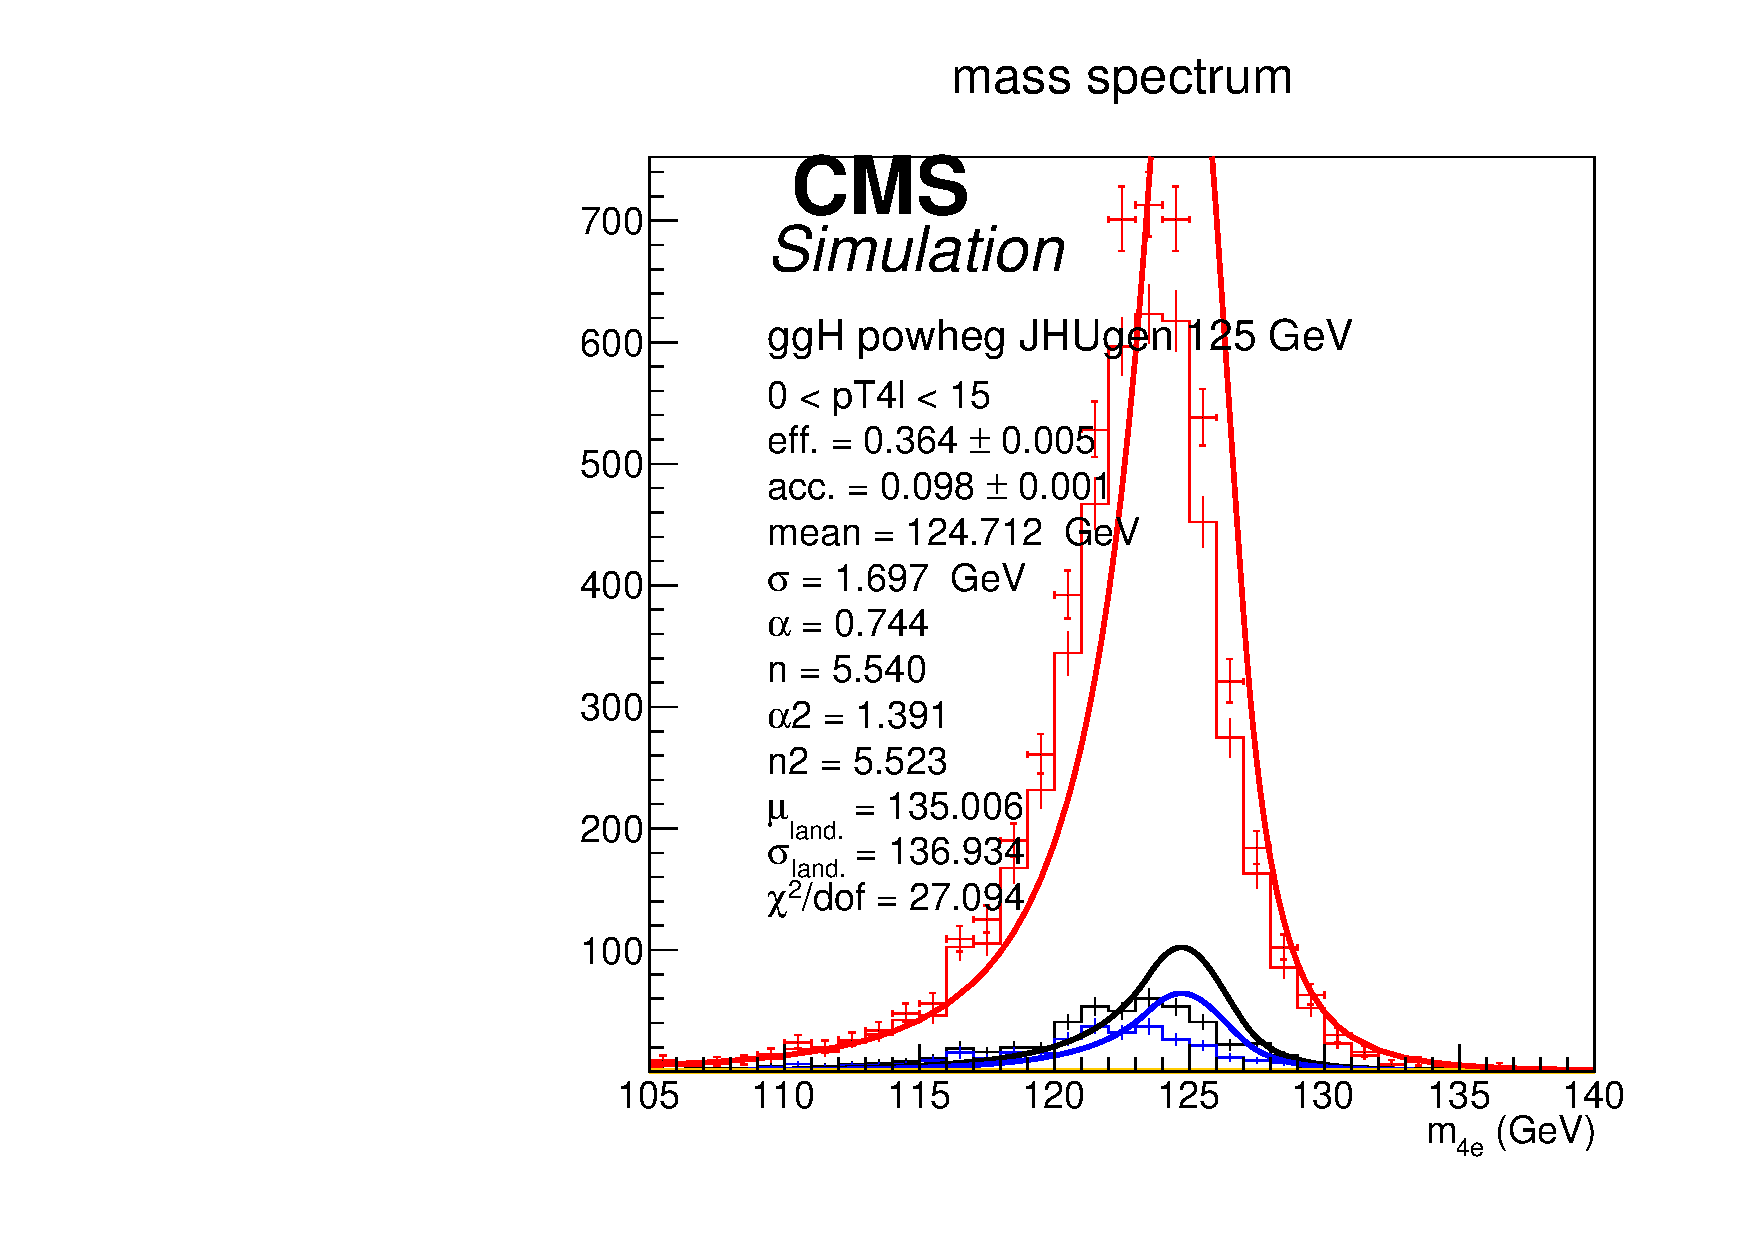
\includegraphics[width=0.3\textwidth,angle=0]{Figures/Appendix//ggH_powheg_JHUgen_125_4e_pT4l_genbin0_recobin0_effs_genWeight*pileupWeight*dataMCWeight.pdf}
      \label{fig:sigfits-pT4l-ggH-powheg15-JHUgen-125-maintext:a}
    }
    \subfigure[$15.0 < \pt(\mathrm{H}) < 30.0$]{
      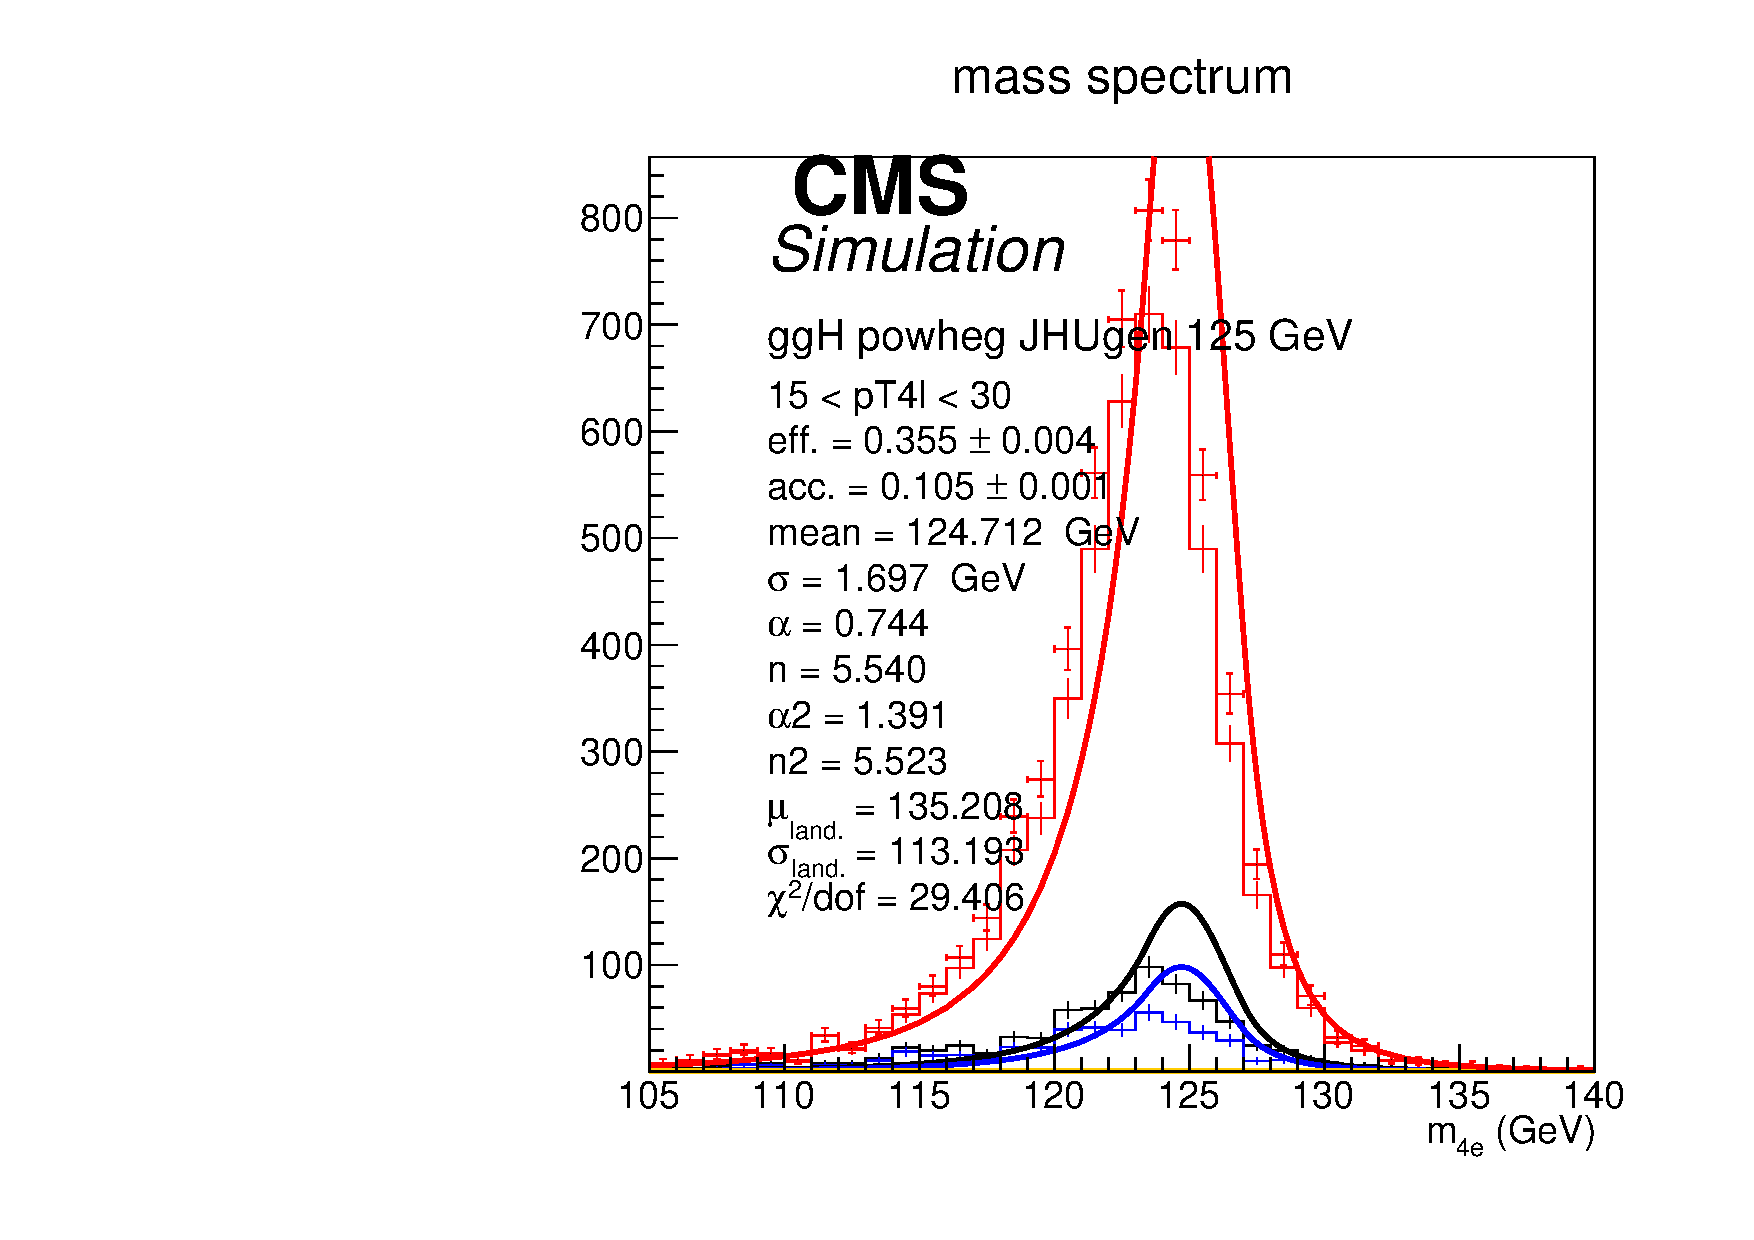
\includegraphics[width=0.3\textwidth,angle=0]{Figures/Appendix//ggH_powheg_JHUgen_125_4e_pT4l_genbin1_recobin1_effs_genWeight*pileupWeight*dataMCWeight.pdf}
      \label{fig:sigfits-pT4l-ggH-powheg15-JHUgen-125-maintext:b}
    }
   \subfigure[$30.0 < \pt(\mathrm{H}) < 45.0$]{
      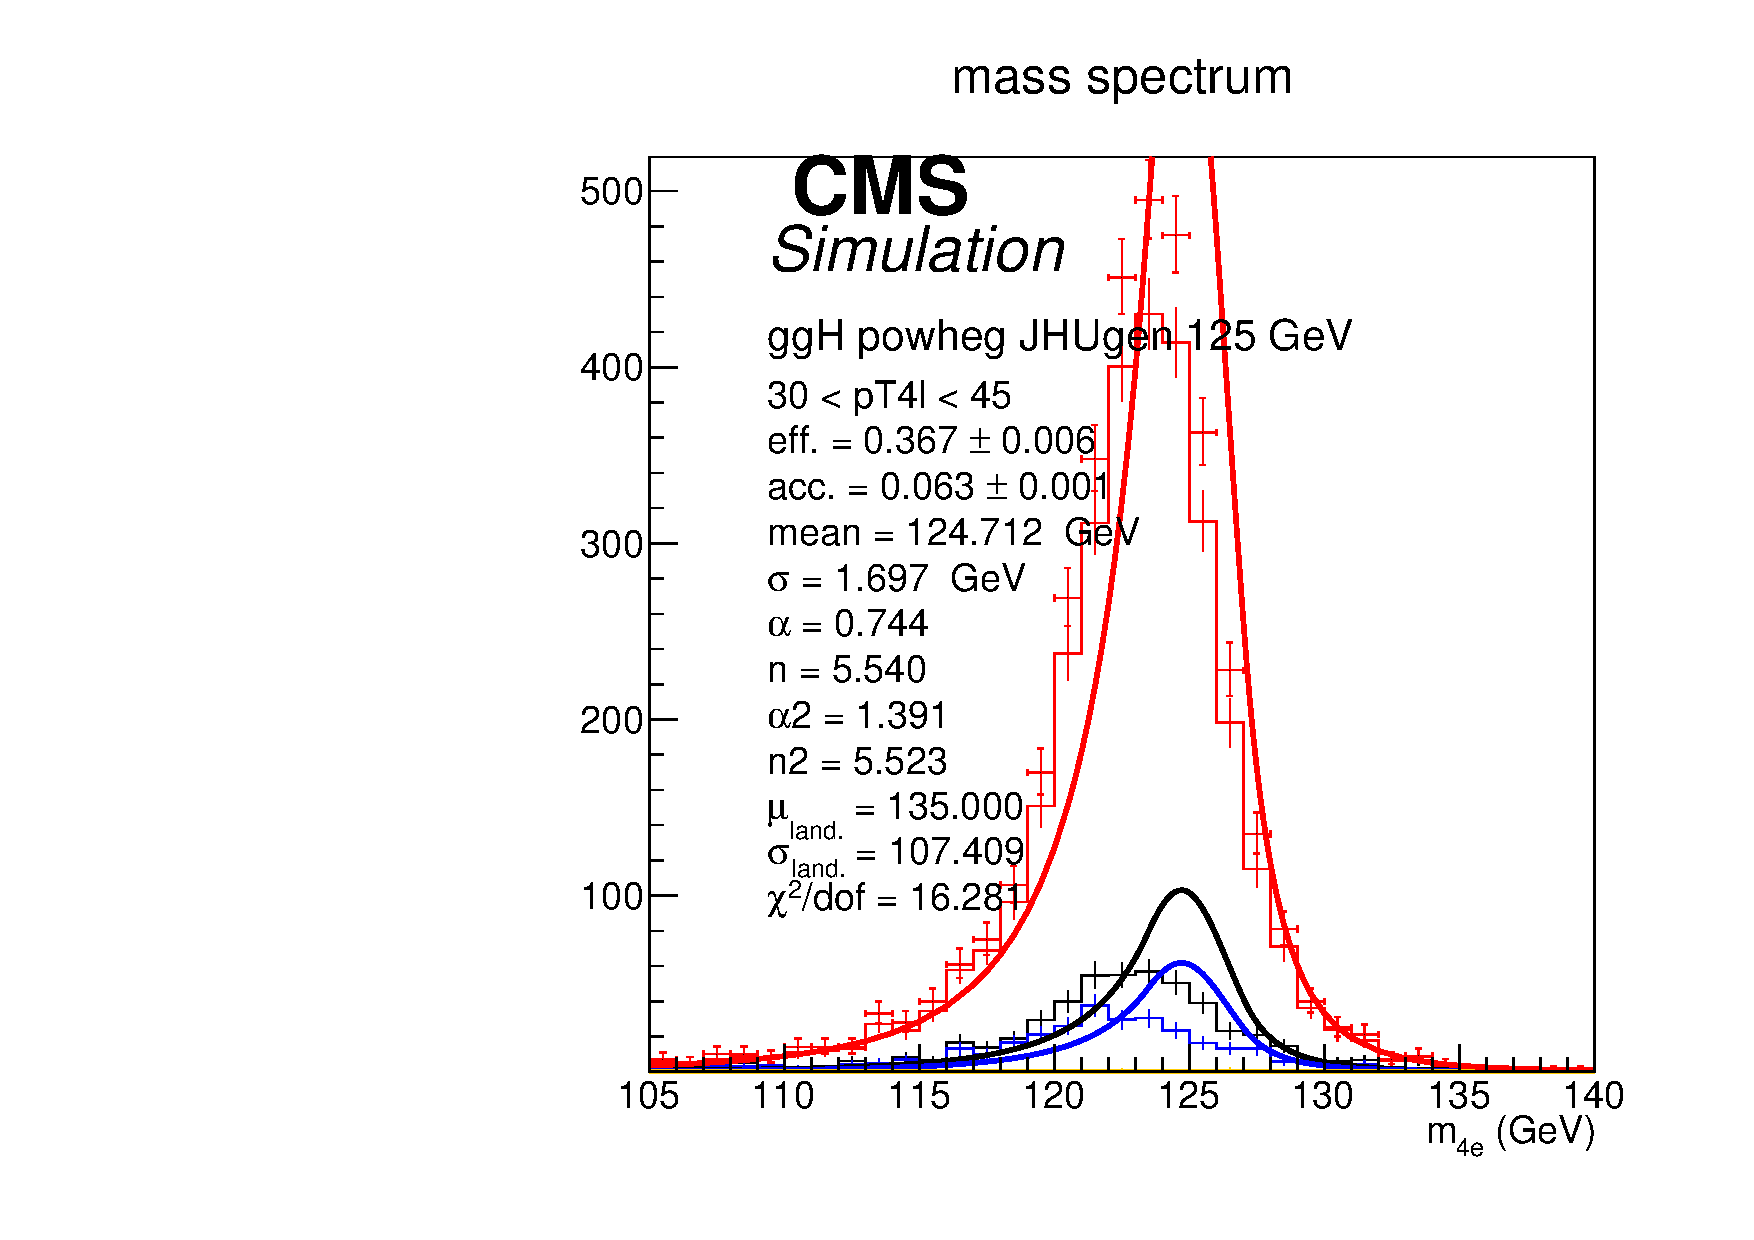
\includegraphics[width=0.3\textwidth,angle=0]{Figures/Appendix//ggH_powheg_JHUgen_125_4e_pT4l_genbin2_recobin2_effs_genWeight*pileupWeight*dataMCWeight.pdf}
      \label{fig:sigfits-pT4l-ggH-powheg15-JHUgen-125-maintext:c}
    }  \\
    \subfigure[$45.0 < \pt(\mathrm{H}) < 80.0$]{
      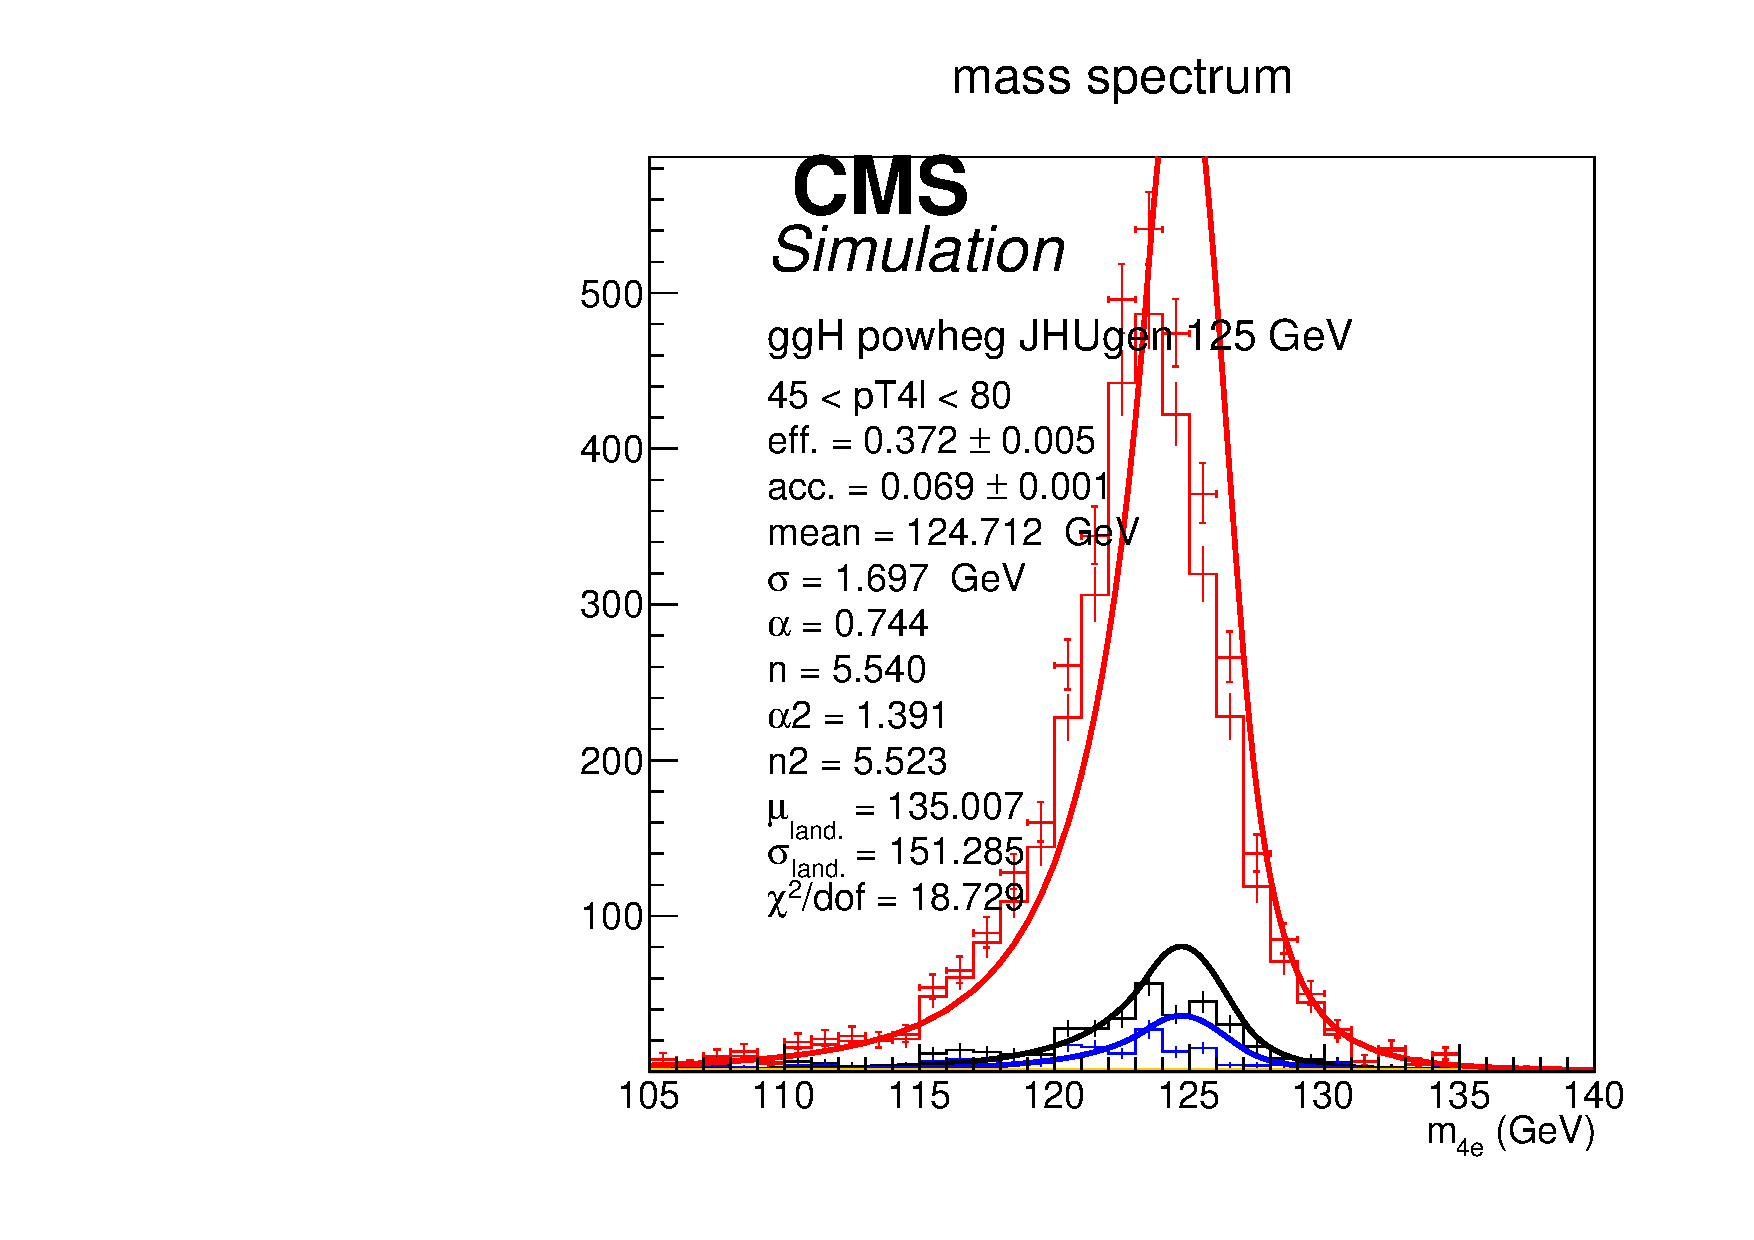
\includegraphics[width=0.3\textwidth,angle=0]{Figures/Appendix//ggH_powheg_JHUgen_125_4e_pT4l_genbin3_recobin3_effs_genWeight*pileupWeight*dataMCWeight.pdf}
      \label{fig:sigfits-pT4l-ggH-powheg15-JHUgen-125-maintext:d}
    }
    \subfigure[$80.0 < \pt(\mathrm{H}) < 120.0$]{
      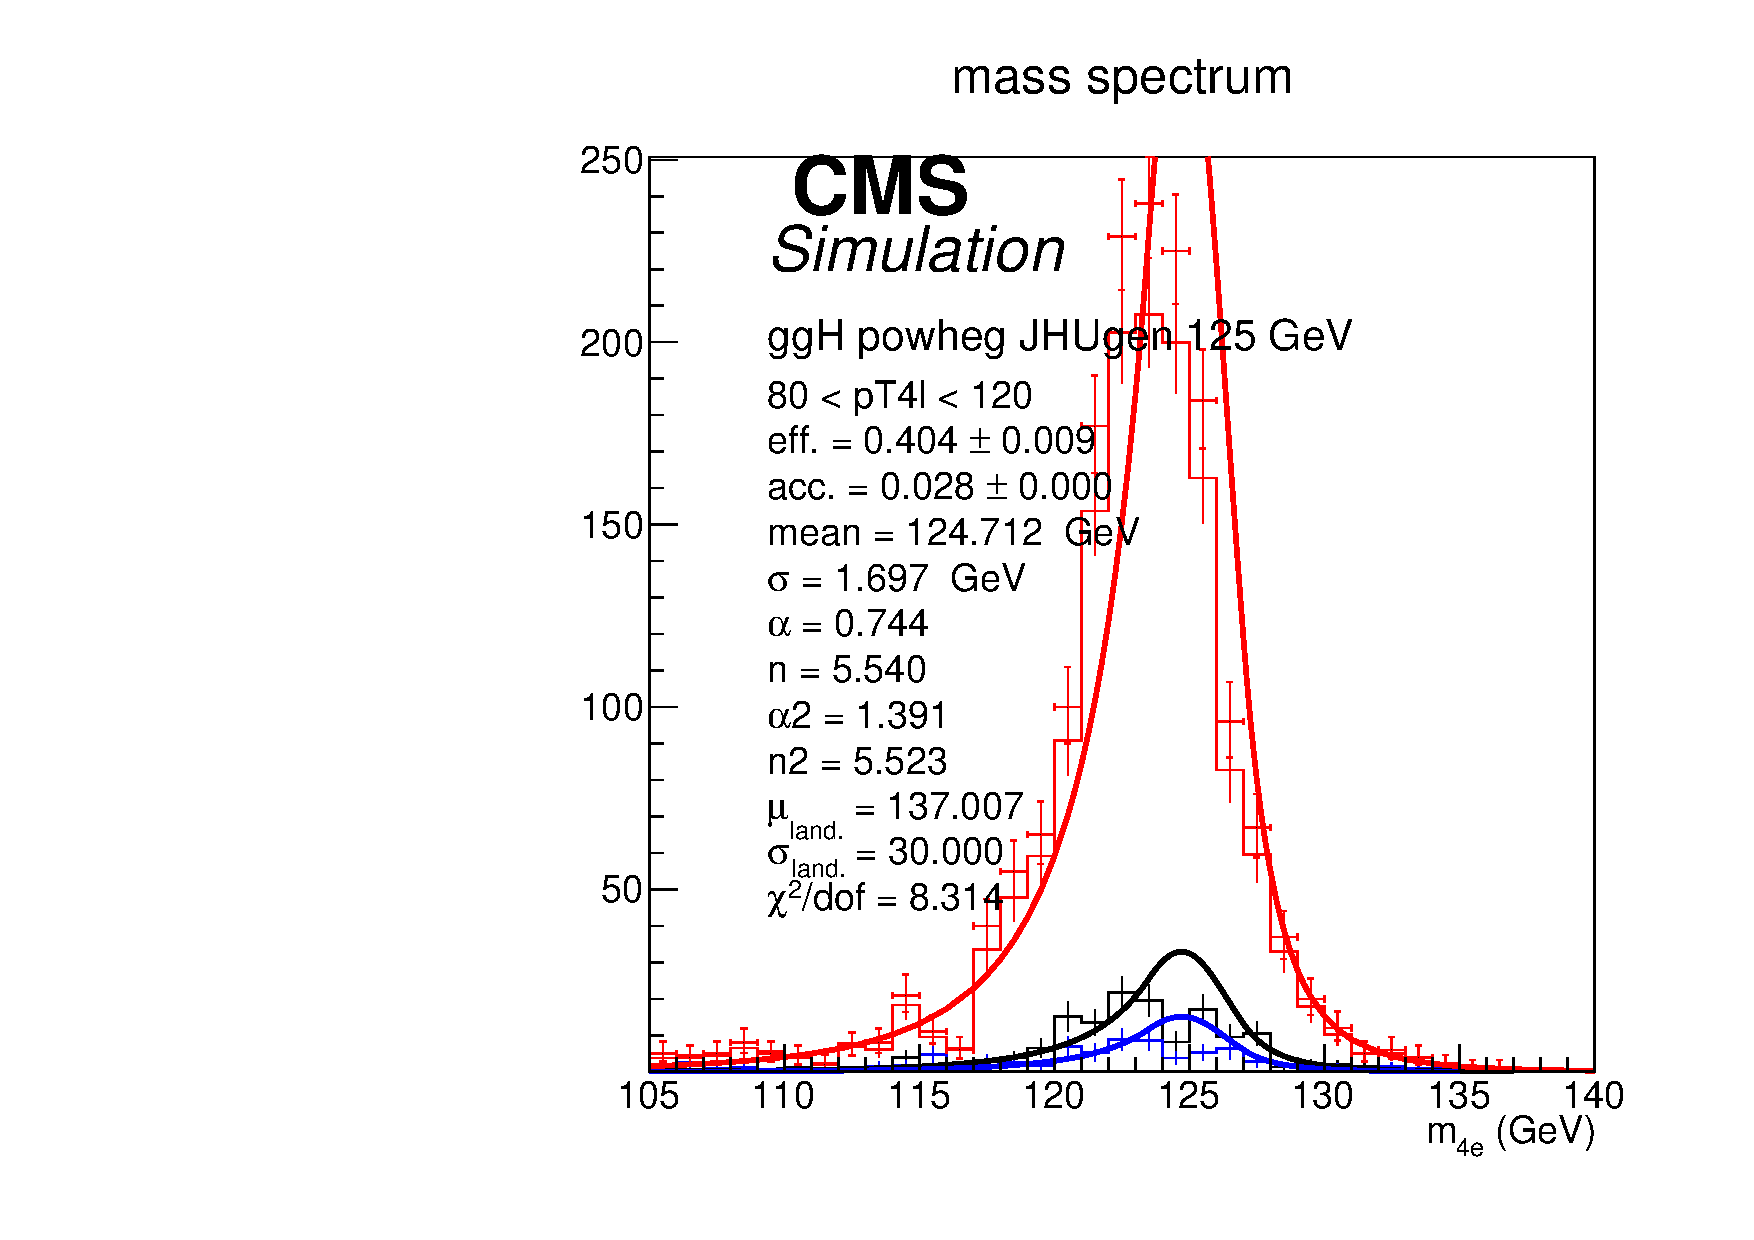
\includegraphics[width=0.3\textwidth,angle=0]{Figures/Appendix//ggH_powheg_JHUgen_125_4e_pT4l_genbin4_recobin4_effs_genWeight*pileupWeight*dataMCWeight.pdf}
      \label{fig:sigfits-pT4l-ggH-powheg15-JHUgen-125-maintext:e}
    }
    \subfigure[$120.0 < \pt(\mathrm{H}) < 200.0$]{
      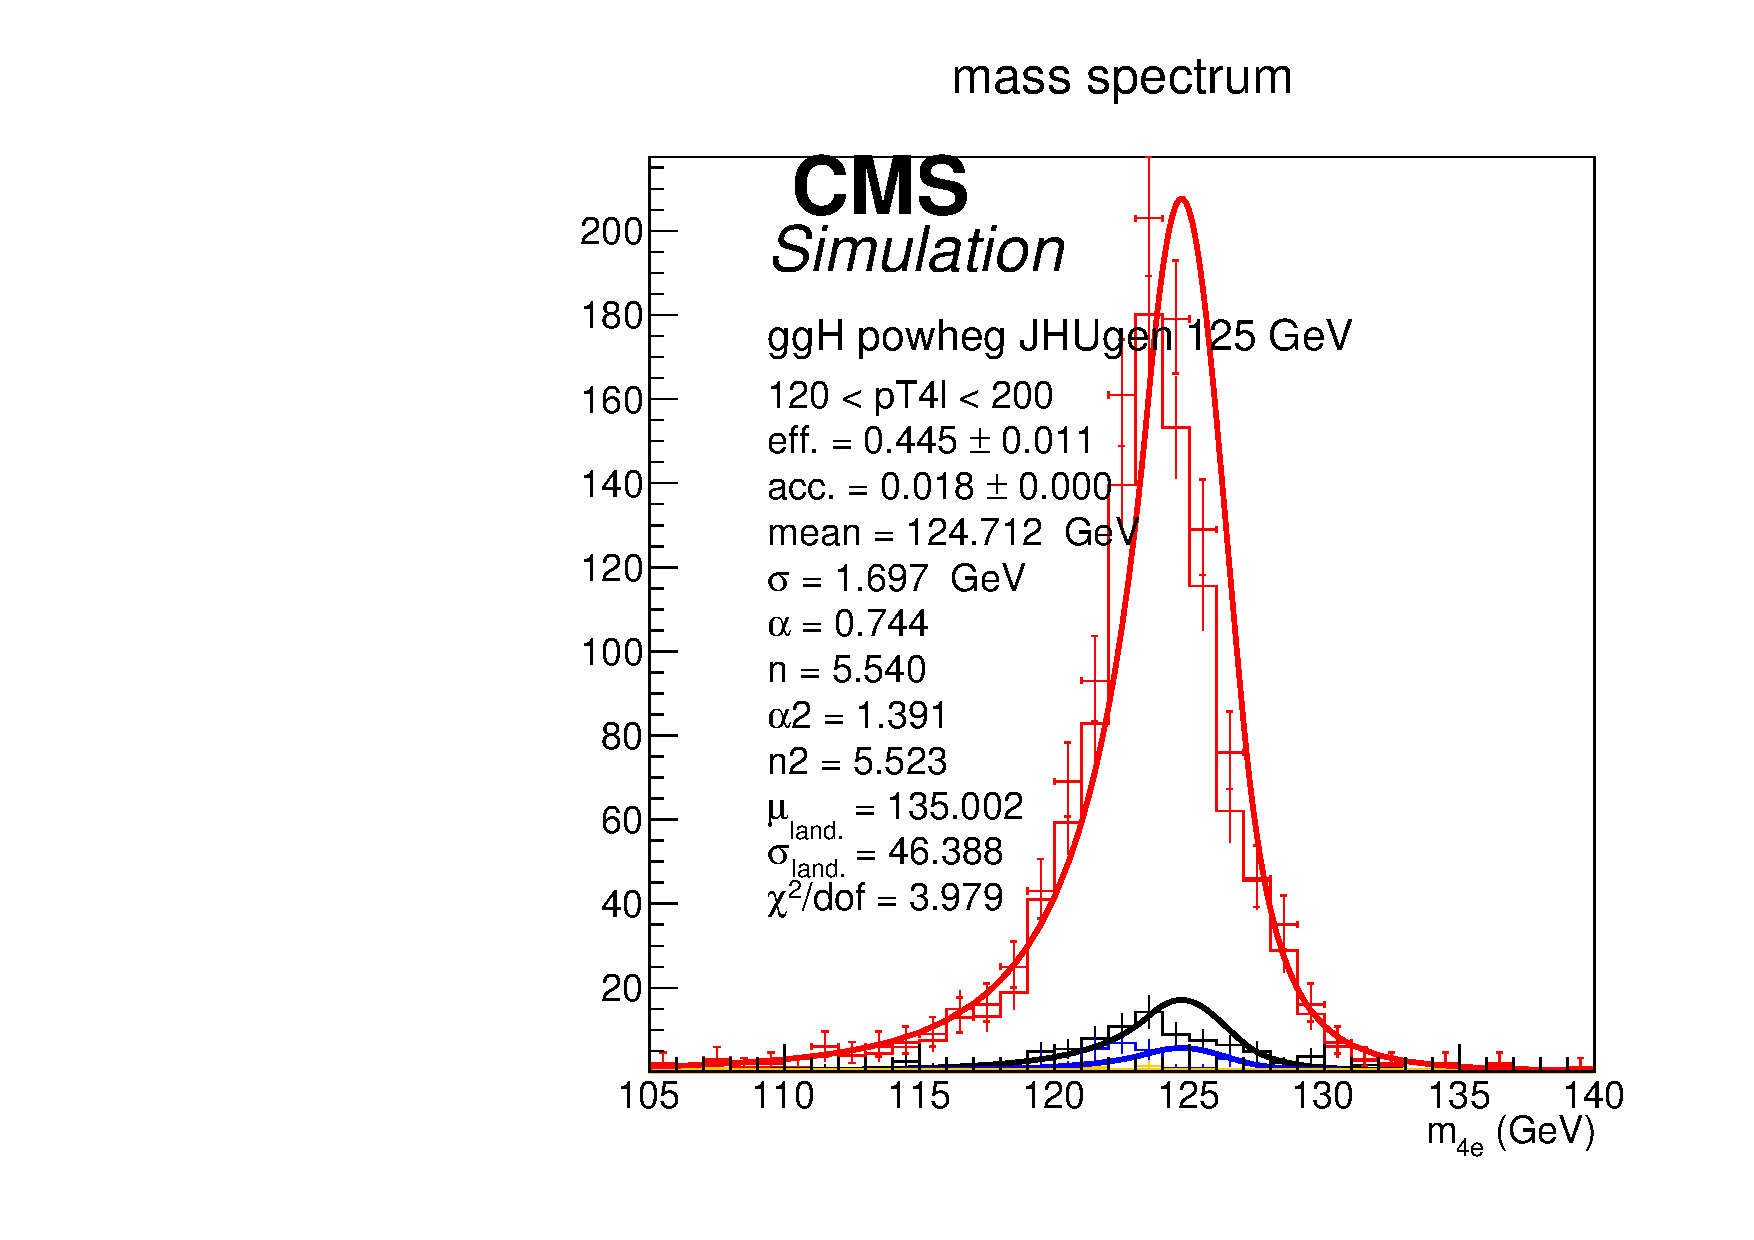
\includegraphics[width=0.3\textwidth,angle=0]{Figures/Appendix//ggH_powheg_JHUgen_125_4e_pT4l_genbin5_recobin5_effs_genWeight*pileupWeight*dataMCWeight.pdf}
      \label{fig:sigfits-pT4l-ggH-powheg15-JHUgen-125-maintext:f}
    } \\
    \subfigure[$200.0 < \pt(\mathrm{H}) < 13000.0$]{
      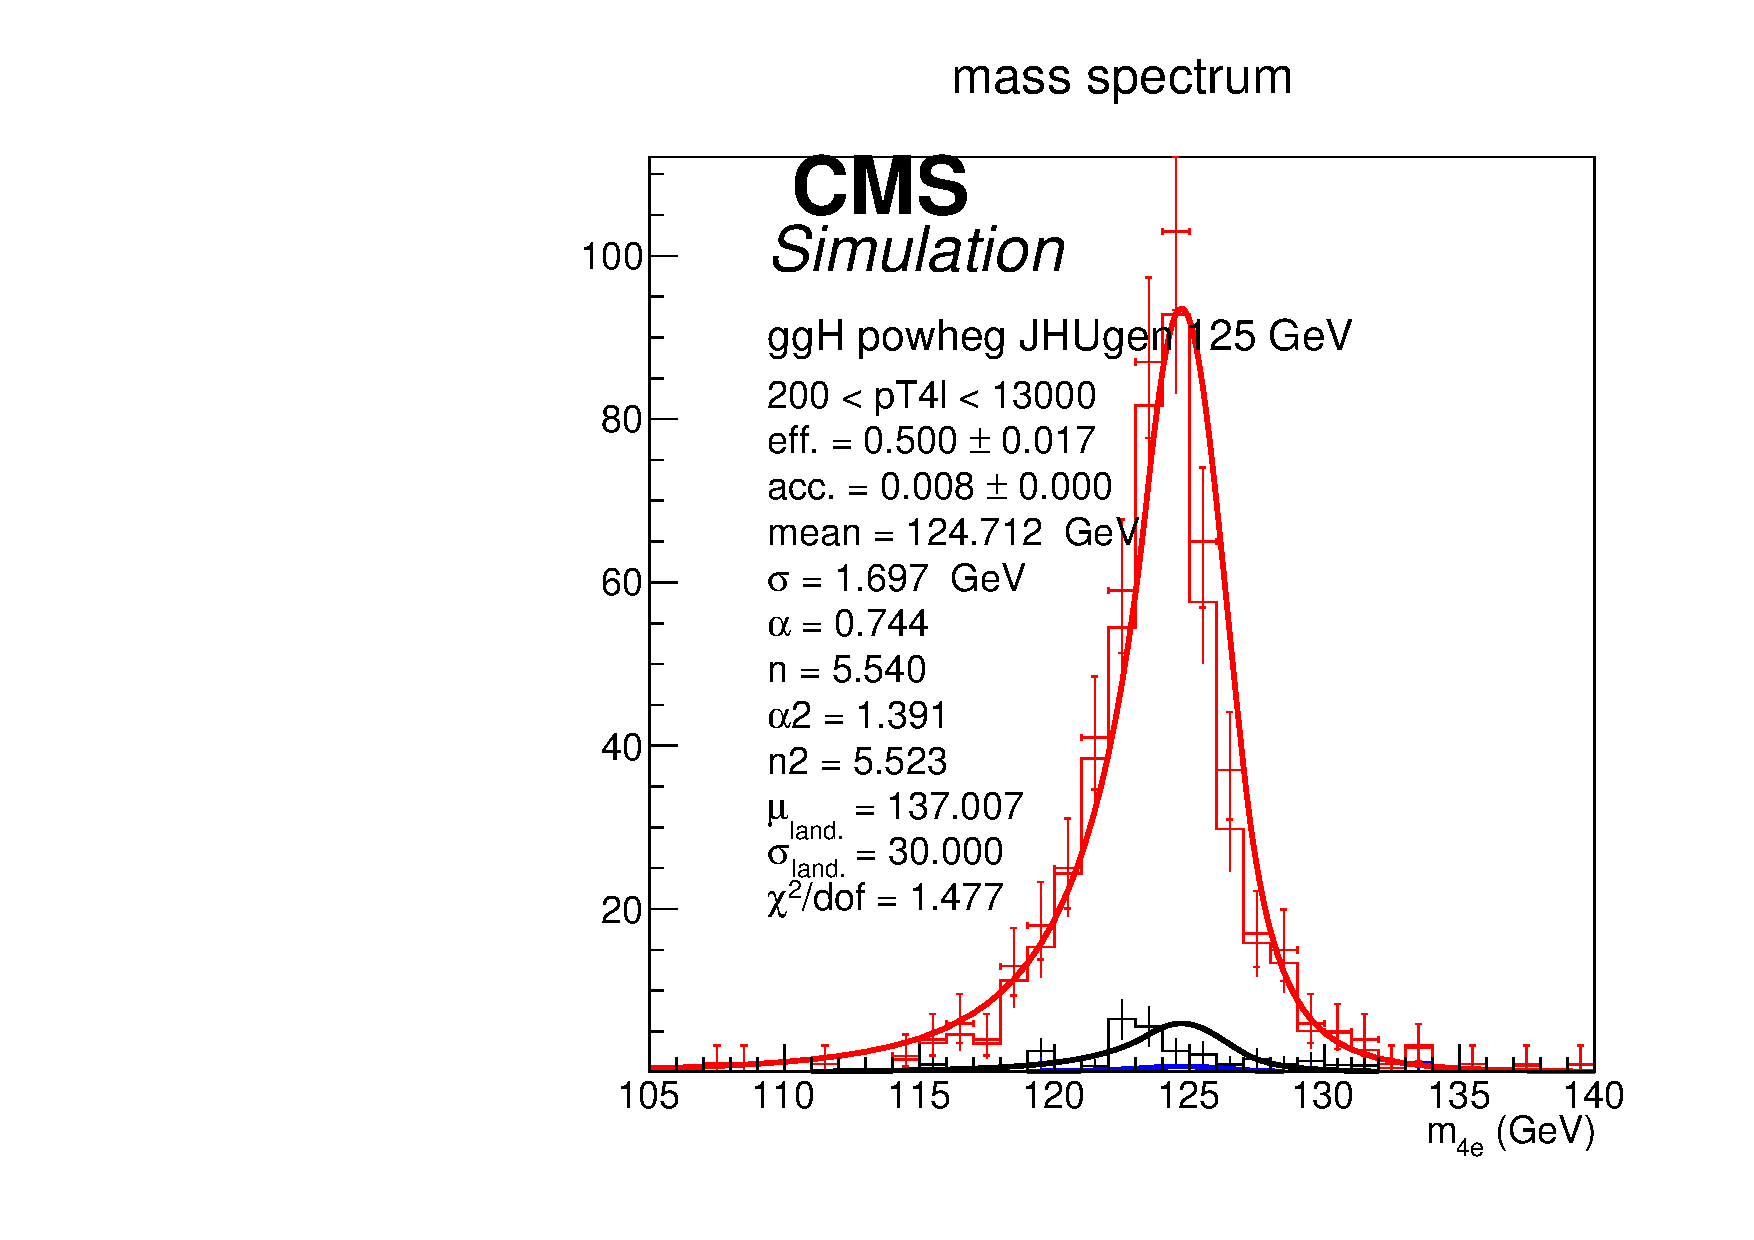
\includegraphics[width=0.3\textwidth,angle=0]{Figures/Appendix//ggH_powheg_JHUgen_125_4e_pT4l_genbin6_recobin6_effs_genWeight*pileupWeight*dataMCWeight.pdf}
      \label{fig:sigfits-pT4l-ggH-powheg15-JHUgen-125-maintext:g}
    }
    \\
    \caption{ Example signal shapes at reconstruction level for a resonance of m(4$\ell$) in $4e$ final state for the $gg\rightarrow \mathrm{H}$ production mode from {\sc powheg+JHUGen} in different bins of $\pt(\mathrm{H})$. The black curve represents events which do not pass the fiducial volume selection. The curve has no effect on the result.
    }
  \label{fig:sigfits-pT4l-ggH-powheg15-JHUgen-125-maintext}
 \end{center}
\end{figure} \clearpage

%% 4mu

\begin{figure}[htb]
  \begin{center}
    \subfigure[$0.0 < \pt(\mathrm{H}) < 15.0 $]{
      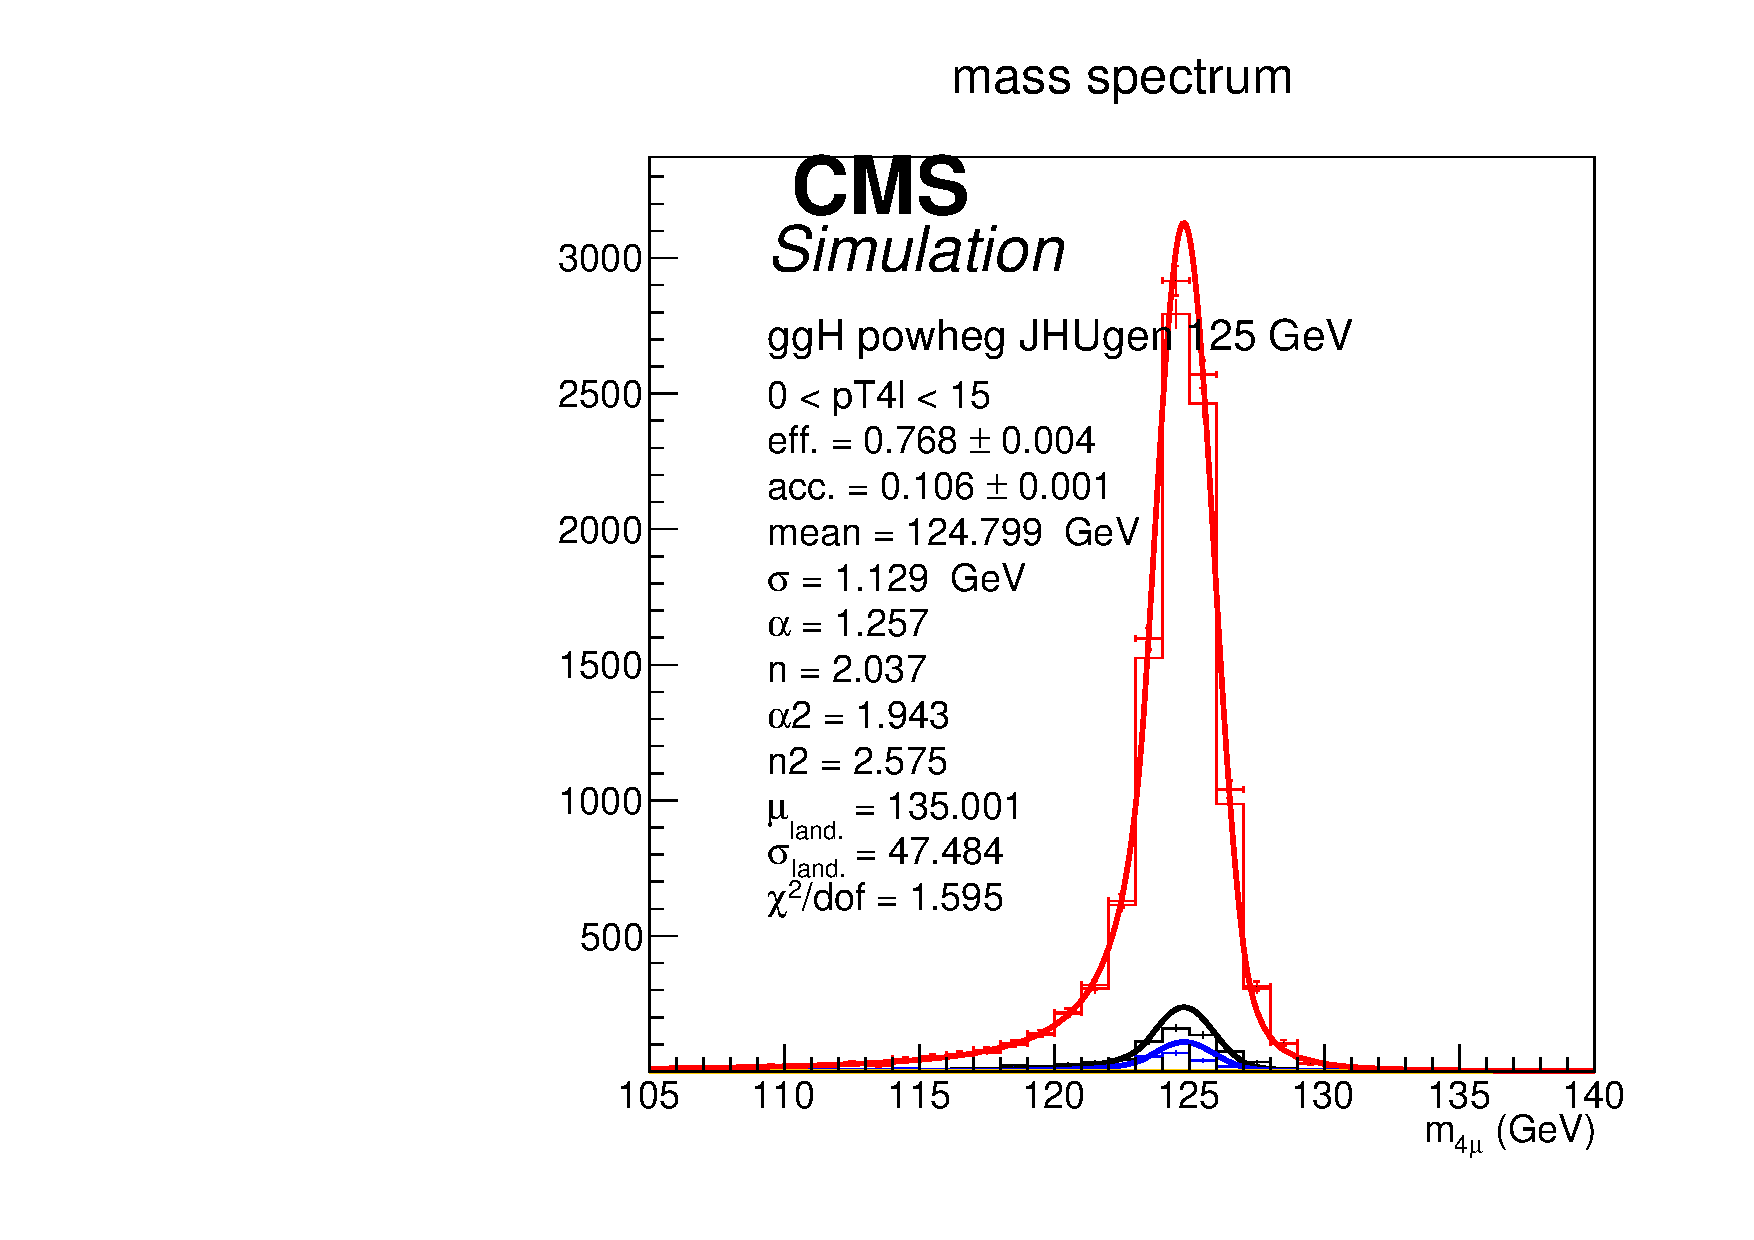
\includegraphics[width=0.3\textwidth,angle=0]{Figures/Appendix//ggH_powheg_JHUgen_125_4mu_pT4l_genbin0_recobin0_effs_genWeight*pileupWeight*dataMCWeight.pdf}
      \label{fig:sigfits-pT4l-ggH-powheg15-JHUgen-125-maintext:a}
    }
    \subfigure[$15.0 < \pt(\mathrm{H}) < 30.0$]{
      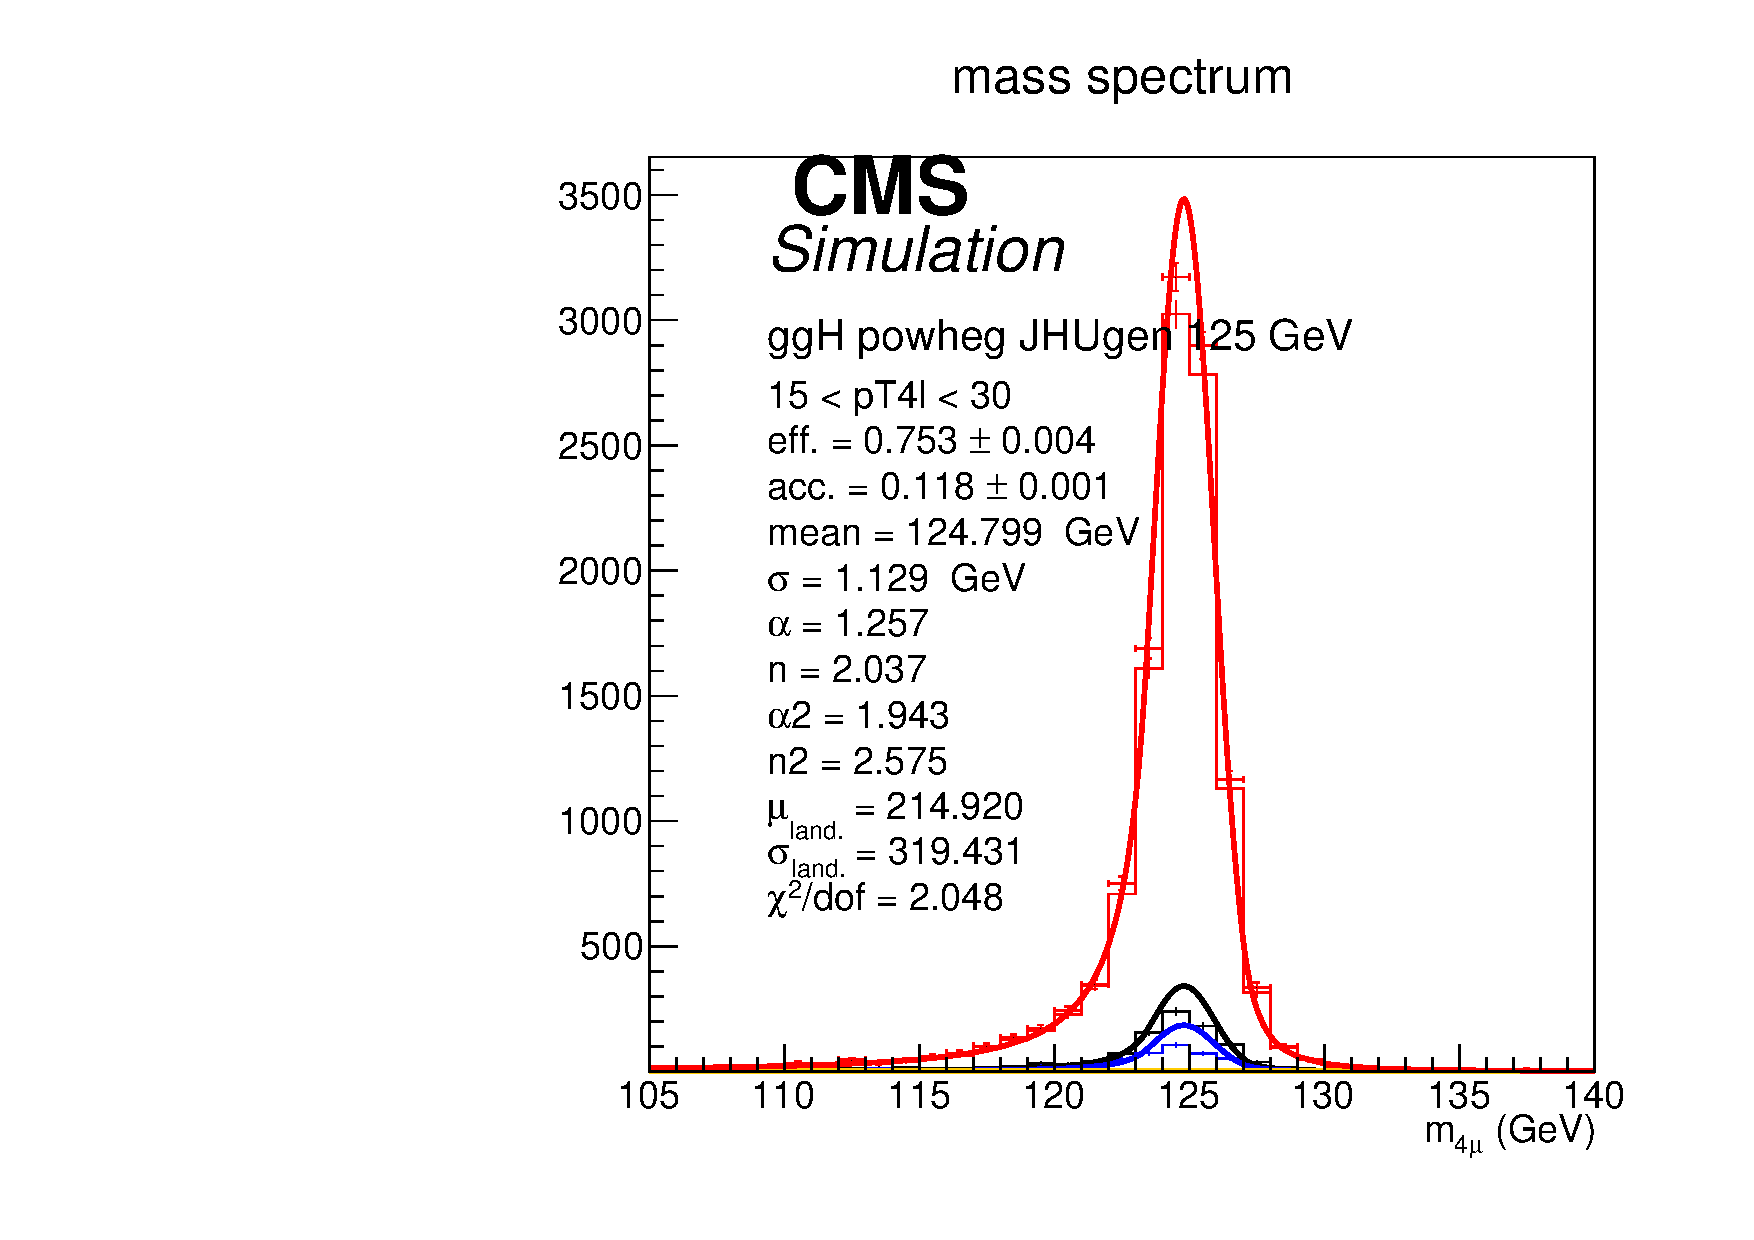
\includegraphics[width=0.3\textwidth,angle=0]{Figures/Appendix//ggH_powheg_JHUgen_125_4mu_pT4l_genbin1_recobin1_effs_genWeight*pileupWeight*dataMCWeight.pdf}
      \label{fig:sigfits-pT4l-ggH-powheg15-JHUgen-125-maintext:b}
    }
   \subfigure[$30.0 < \pt(\mathrm{H}) < 45.0$]{
      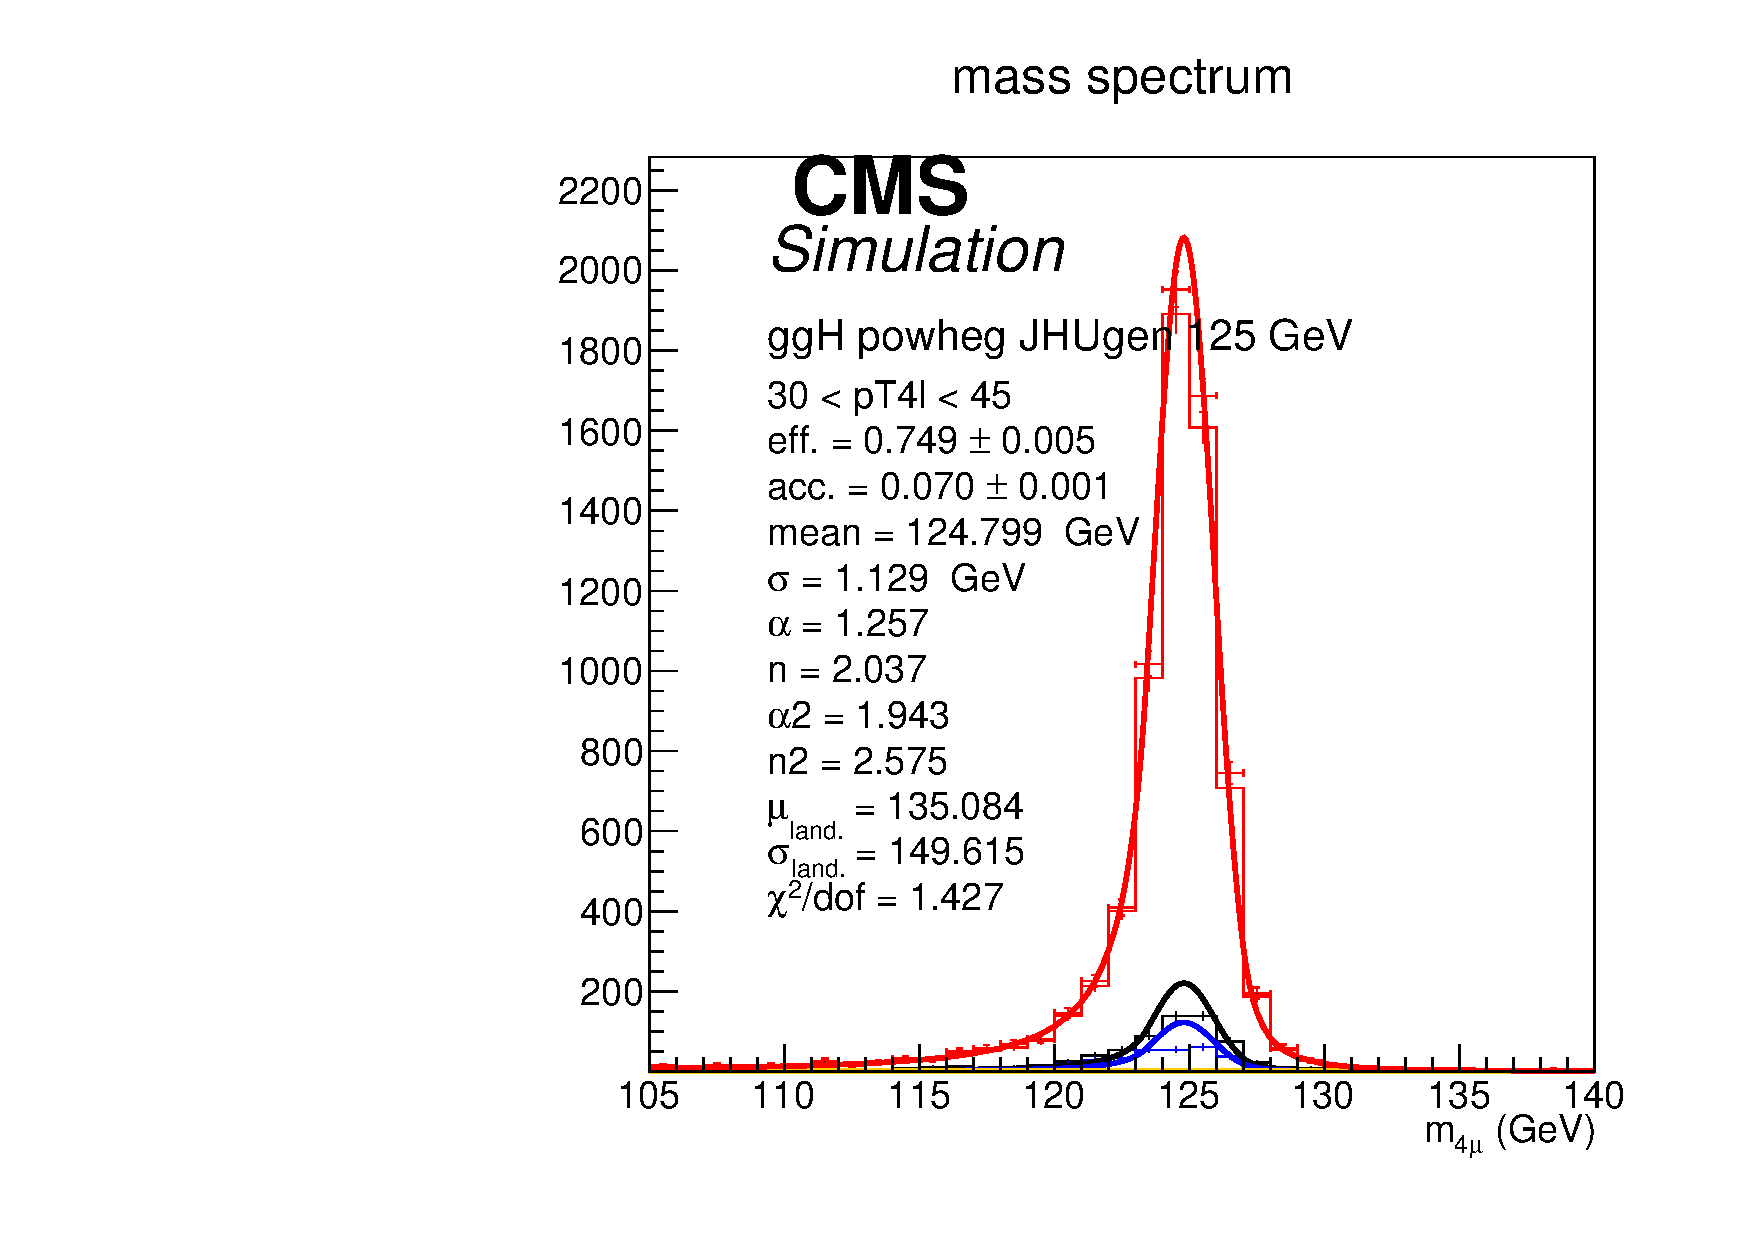
\includegraphics[width=0.3\textwidth,angle=0]{Figures/Appendix//ggH_powheg_JHUgen_125_4mu_pT4l_genbin2_recobin2_effs_genWeight*pileupWeight*dataMCWeight.pdf}
      \label{fig:sigfits-pT4l-ggH-powheg15-JHUgen-125-maintext:c}
    }  \\
    \subfigure[$45.0 < \pt(\mathrm{H}) < 80.0$]{
      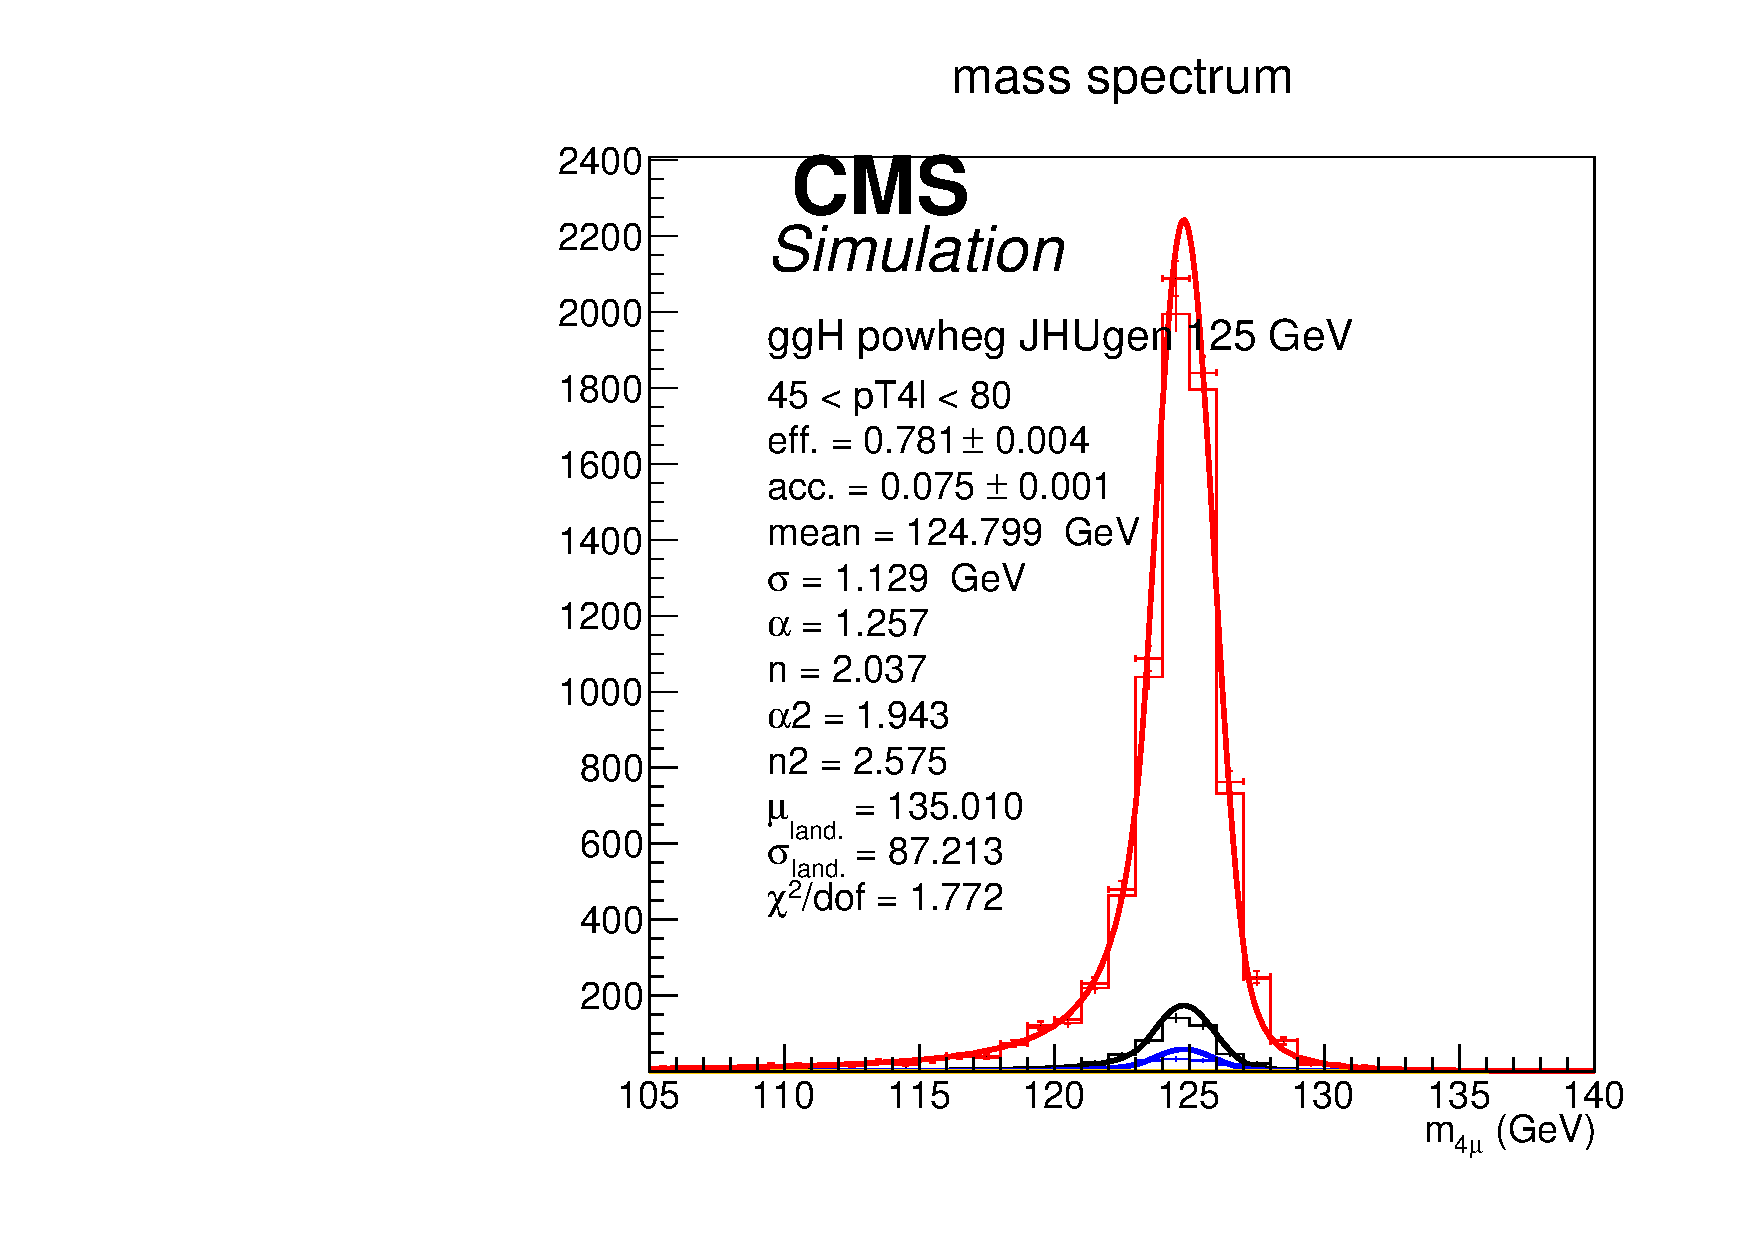
\includegraphics[width=0.3\textwidth,angle=0]{Figures/Appendix//ggH_powheg_JHUgen_125_4mu_pT4l_genbin3_recobin3_effs_genWeight*pileupWeight*dataMCWeight.pdf}
      \label{fig:sigfits-pT4l-ggH-powheg15-JHUgen-125-maintext:d}
    }
    \subfigure[$80.0 < \pt(\mathrm{H}) < 120.0$]{
      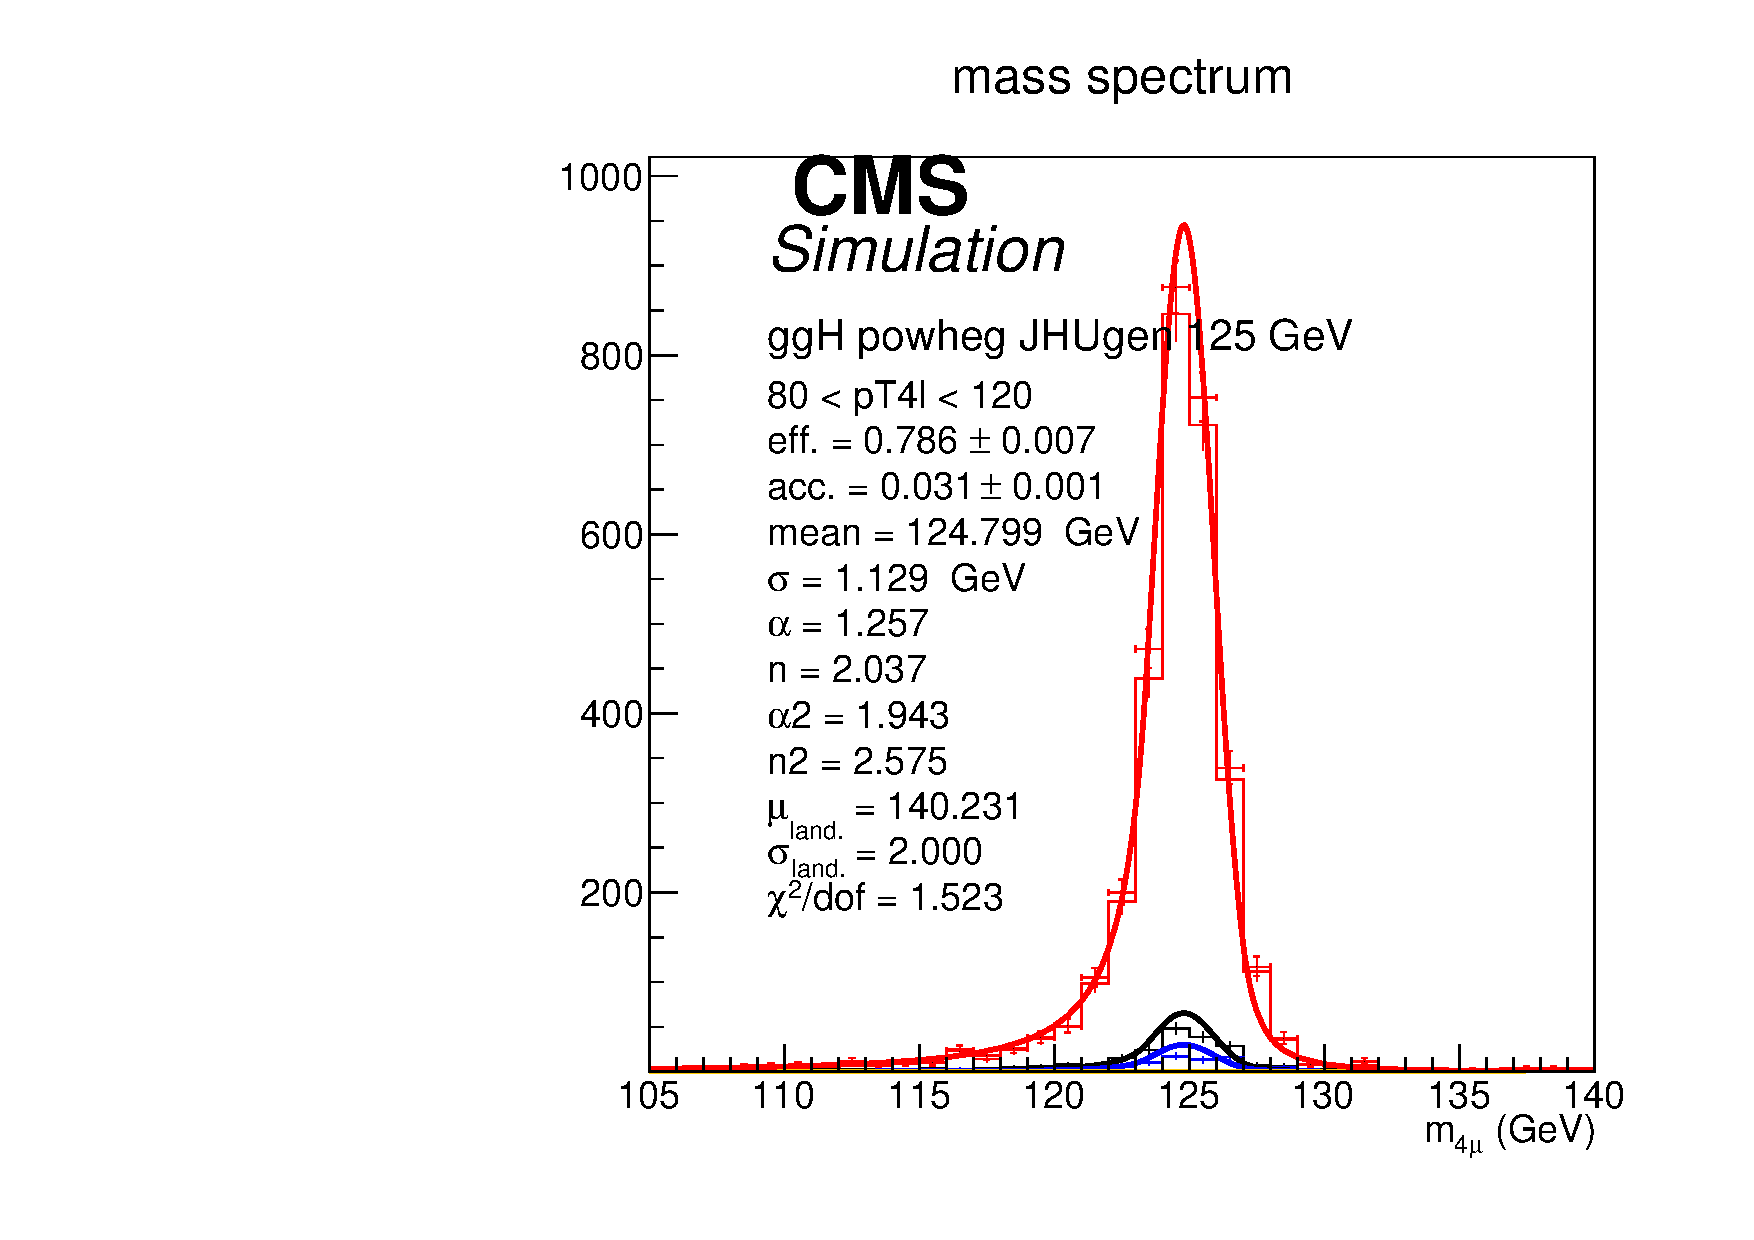
\includegraphics[width=0.3\textwidth,angle=0]{Figures/Appendix//ggH_powheg_JHUgen_125_4mu_pT4l_genbin4_recobin4_effs_genWeight*pileupWeight*dataMCWeight.pdf}
      \label{fig:sigfits-pT4l-ggH-powheg15-JHUgen-125-maintext:e}
    }
    \subfigure[$120.0 < \pt(\mathrm{H}) < 200.0$]{
      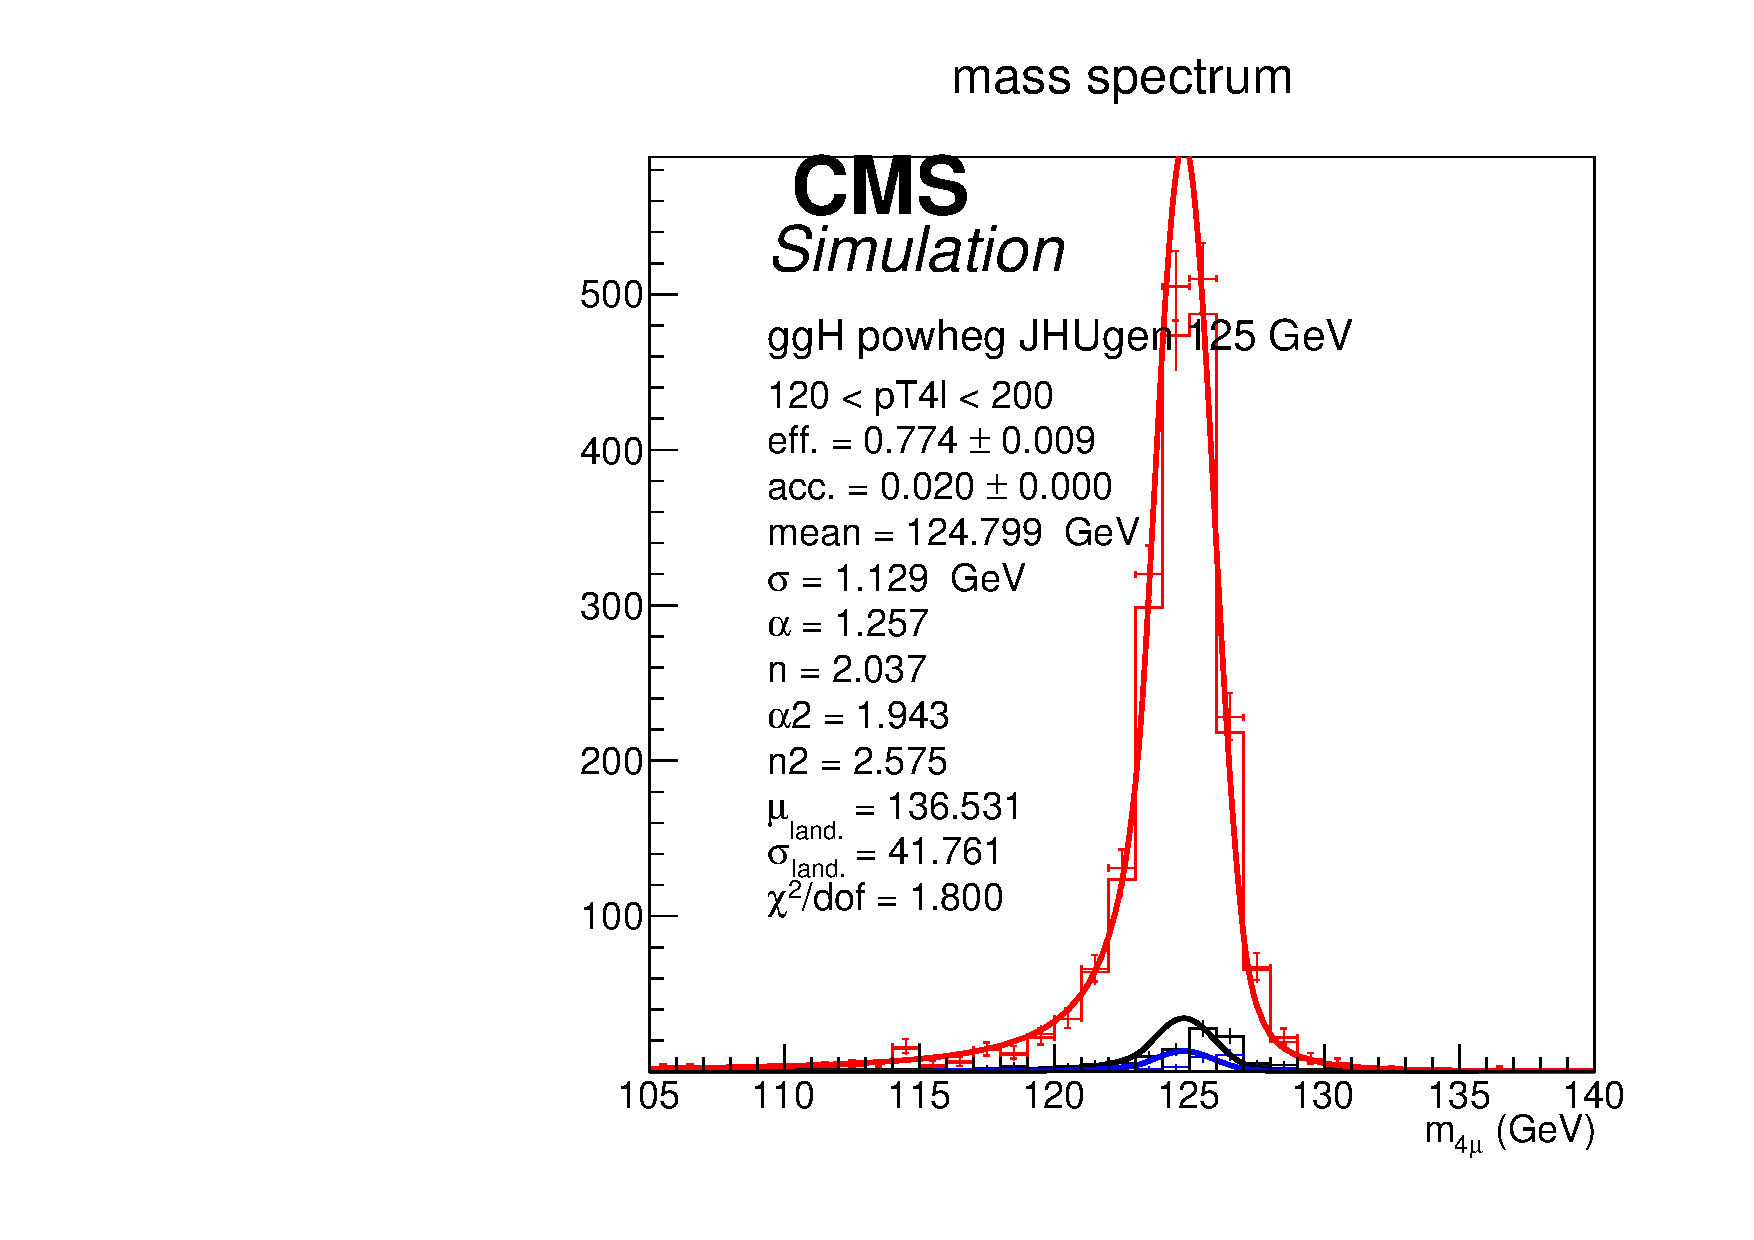
\includegraphics[width=0.3\textwidth,angle=0]{Figures/Appendix//ggH_powheg_JHUgen_125_4mu_pT4l_genbin5_recobin5_effs_genWeight*pileupWeight*dataMCWeight.pdf}
      \label{fig:sigfits-pT4l-ggH-powheg15-JHUgen-125-maintext:f}
    } \\
    \subfigure[$200.0 < \pt(\mathrm{H}) < 13000.0$]{
      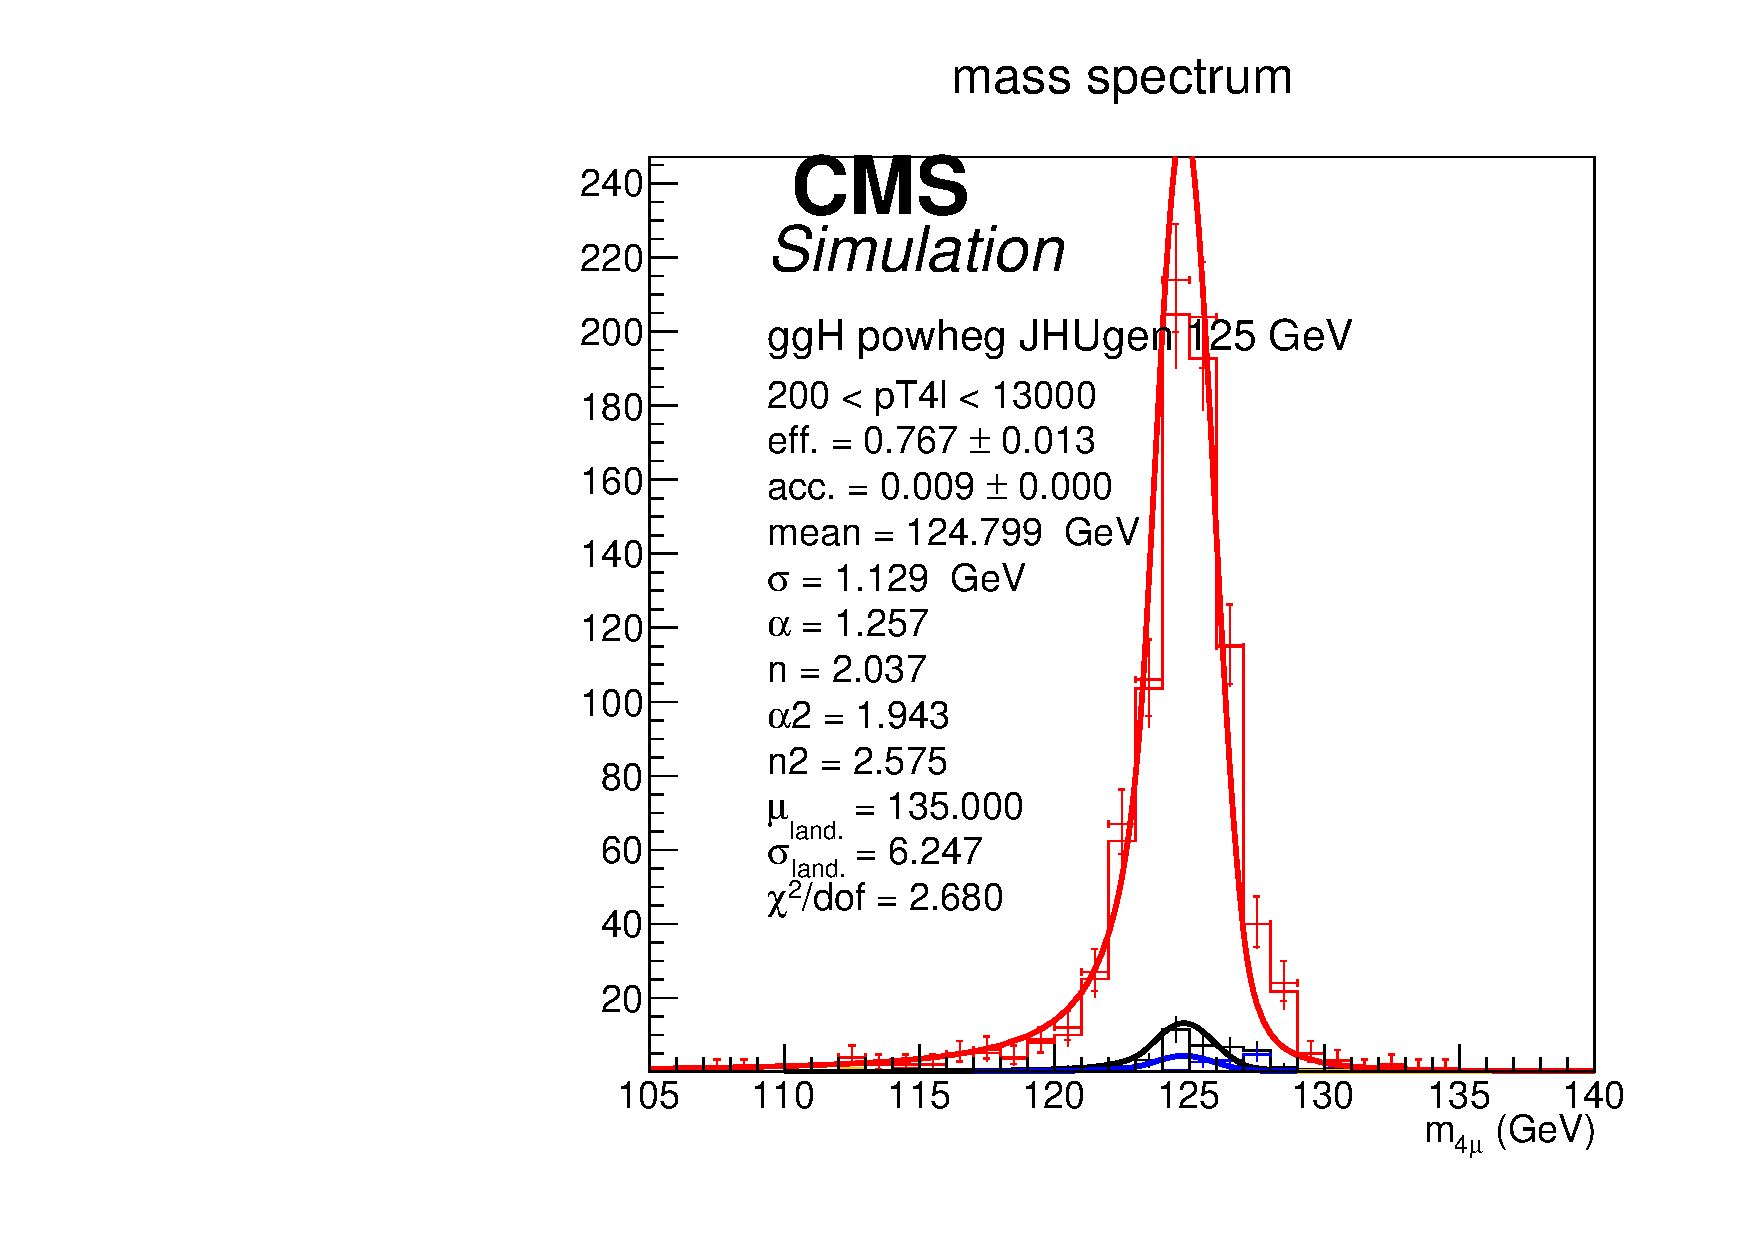
\includegraphics[width=0.3\textwidth,angle=0]{Figures/Appendix//ggH_powheg_JHUgen_125_4mu_pT4l_genbin6_recobin6_effs_genWeight*pileupWeight*dataMCWeight.pdf}
      \label{fig:sigfits-pT4l-ggH-powheg15-JHUgen-125-maintext:g}
    }
    \\
    \caption{ Example signal shapes at reconstruction level for a resonance of m(4$\ell$) in $4\mu$ final state for the $gg\rightarrow \mathrm{H}$ production mode from {\sc powheg+JHUGen} in different bins of $\pt(\mathrm{H})$. The black curve represents events which do not pass the fiducial volume selection. The curve has no effect on the result.
    }
  \label{fig:sigfits-pT4l-ggH-powheg15-JHUgen-125-maintext}
 \end{center}
\end{figure} \clearpage


%%%%%%%%%%%%%%%%%%%%%%%%%%%%%%%%%%%%%%%%%%%%%%%%%%%%%%%%%%%%% VBF %%%%%%%%%%%%%%%%%%%%%%%

\begin{figure}[htb]
  \begin{center}
    \subfigure[$0.0 < \pt(\mathrm{H}) < 15.0 $]{
      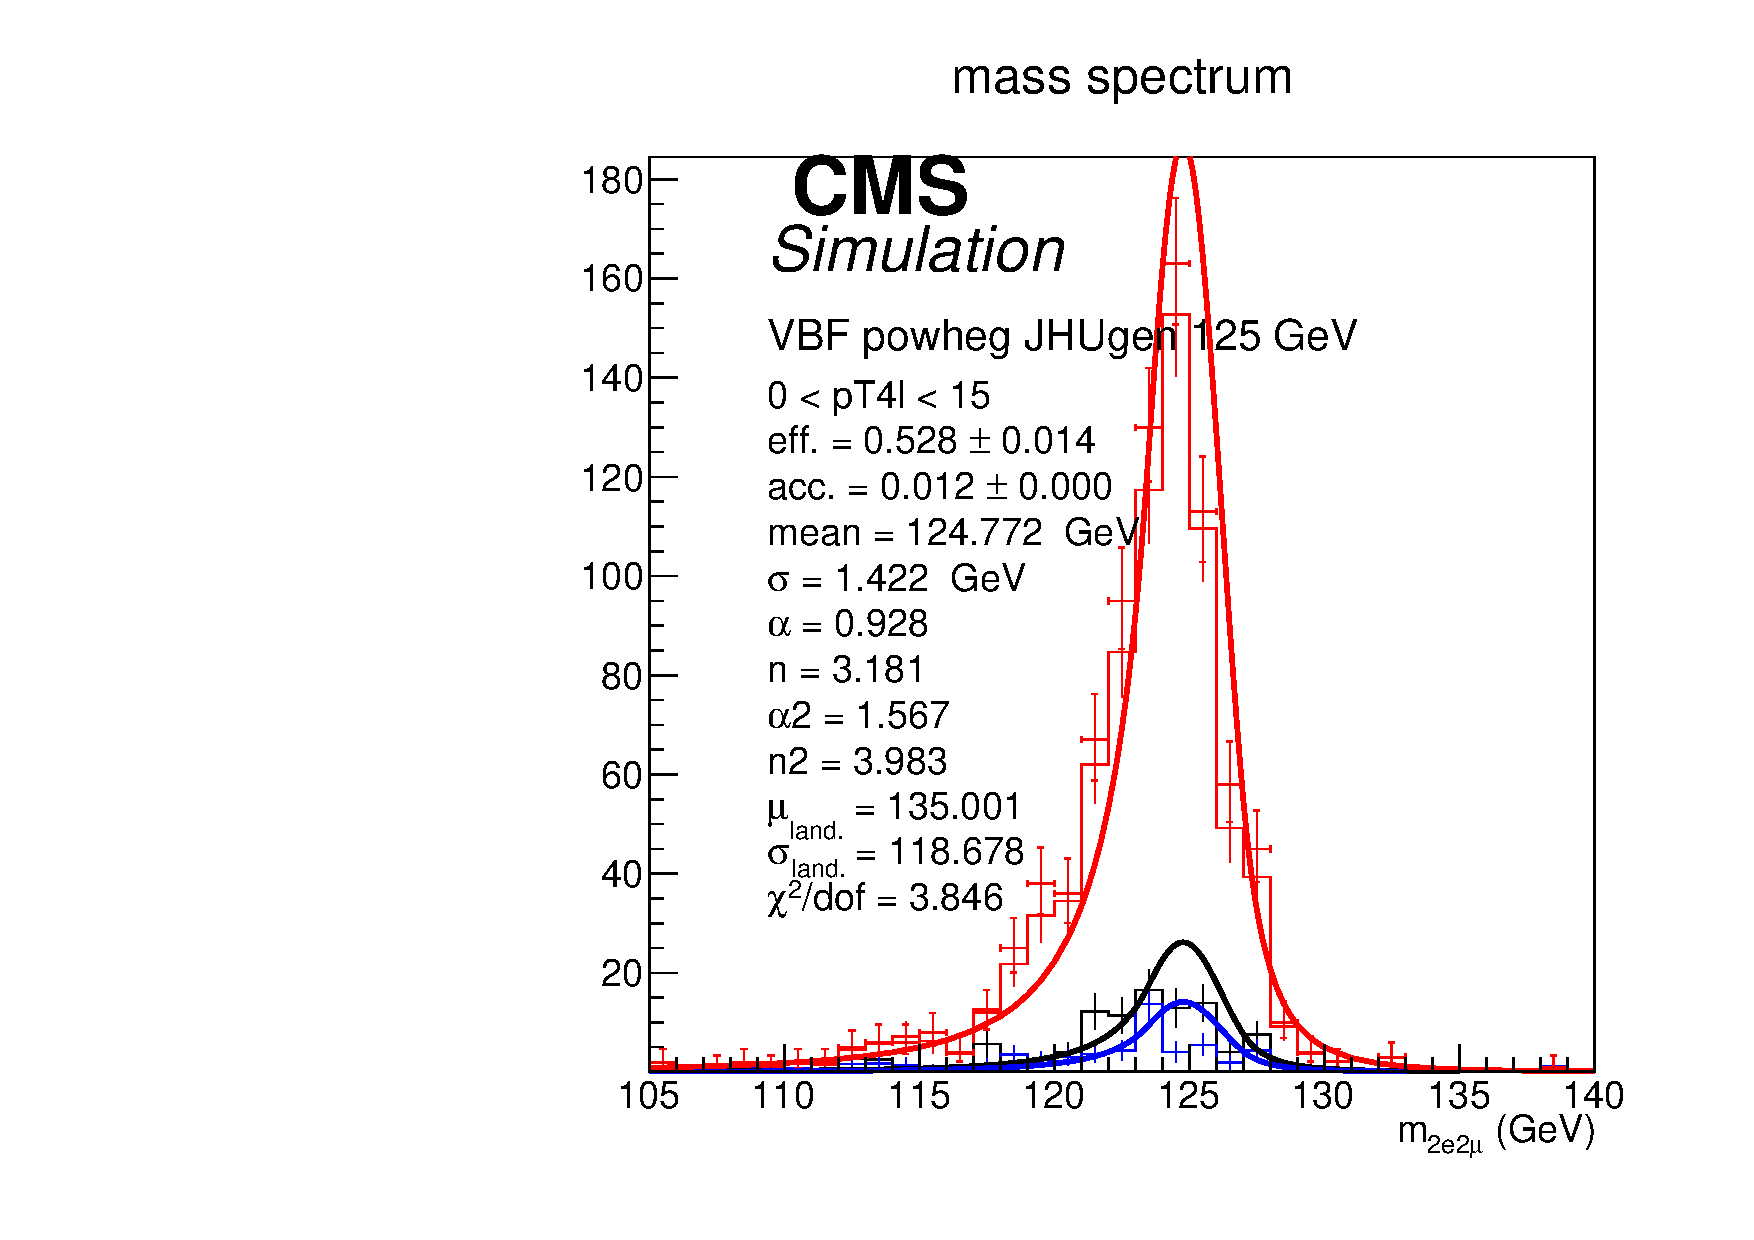
\includegraphics[width=0.3\textwidth,angle=0]{Figures/Appendix//VBF_powheg_JHUgen_125_2e2mu_pT4l_genbin0_recobin0_effs_genWeight*pileupWeight*dataMCWeight.pdf}
      \label{fig:sigfits-pT4l-VBF-powheg15-JHUgen-125-maintext:a}
    }
    \subfigure[$15.0 < \pt(\mathrm{H}) < 30.0$]{
      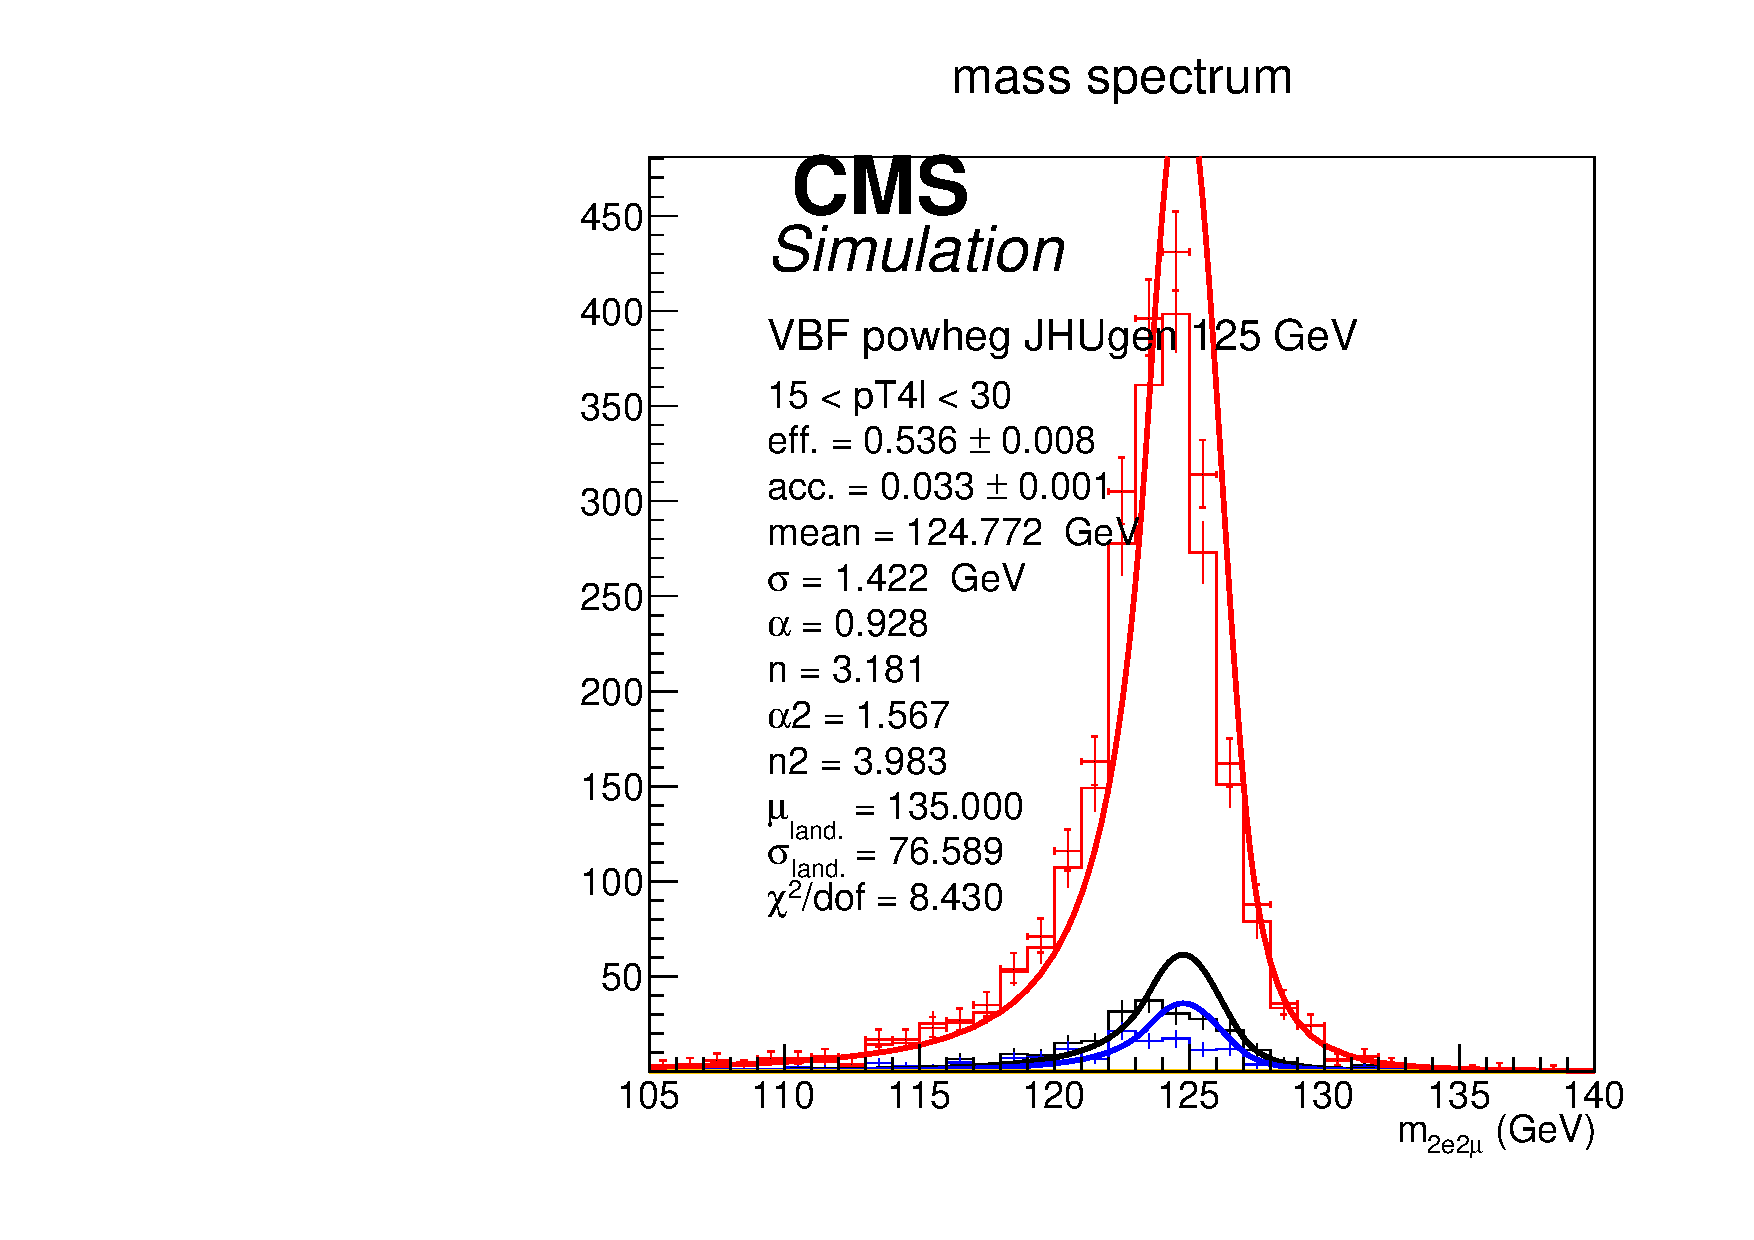
\includegraphics[width=0.3\textwidth,angle=0]{Figures/Appendix//VBF_powheg_JHUgen_125_2e2mu_pT4l_genbin1_recobin1_effs_genWeight*pileupWeight*dataMCWeight.pdf}
      \label{fig:sigfits-pT4l-VBF-powheg15-JHUgen-125-maintext:b}
    }
   \subfigure[$30.0 < \pt(\mathrm{H}) < 45.0$]{
      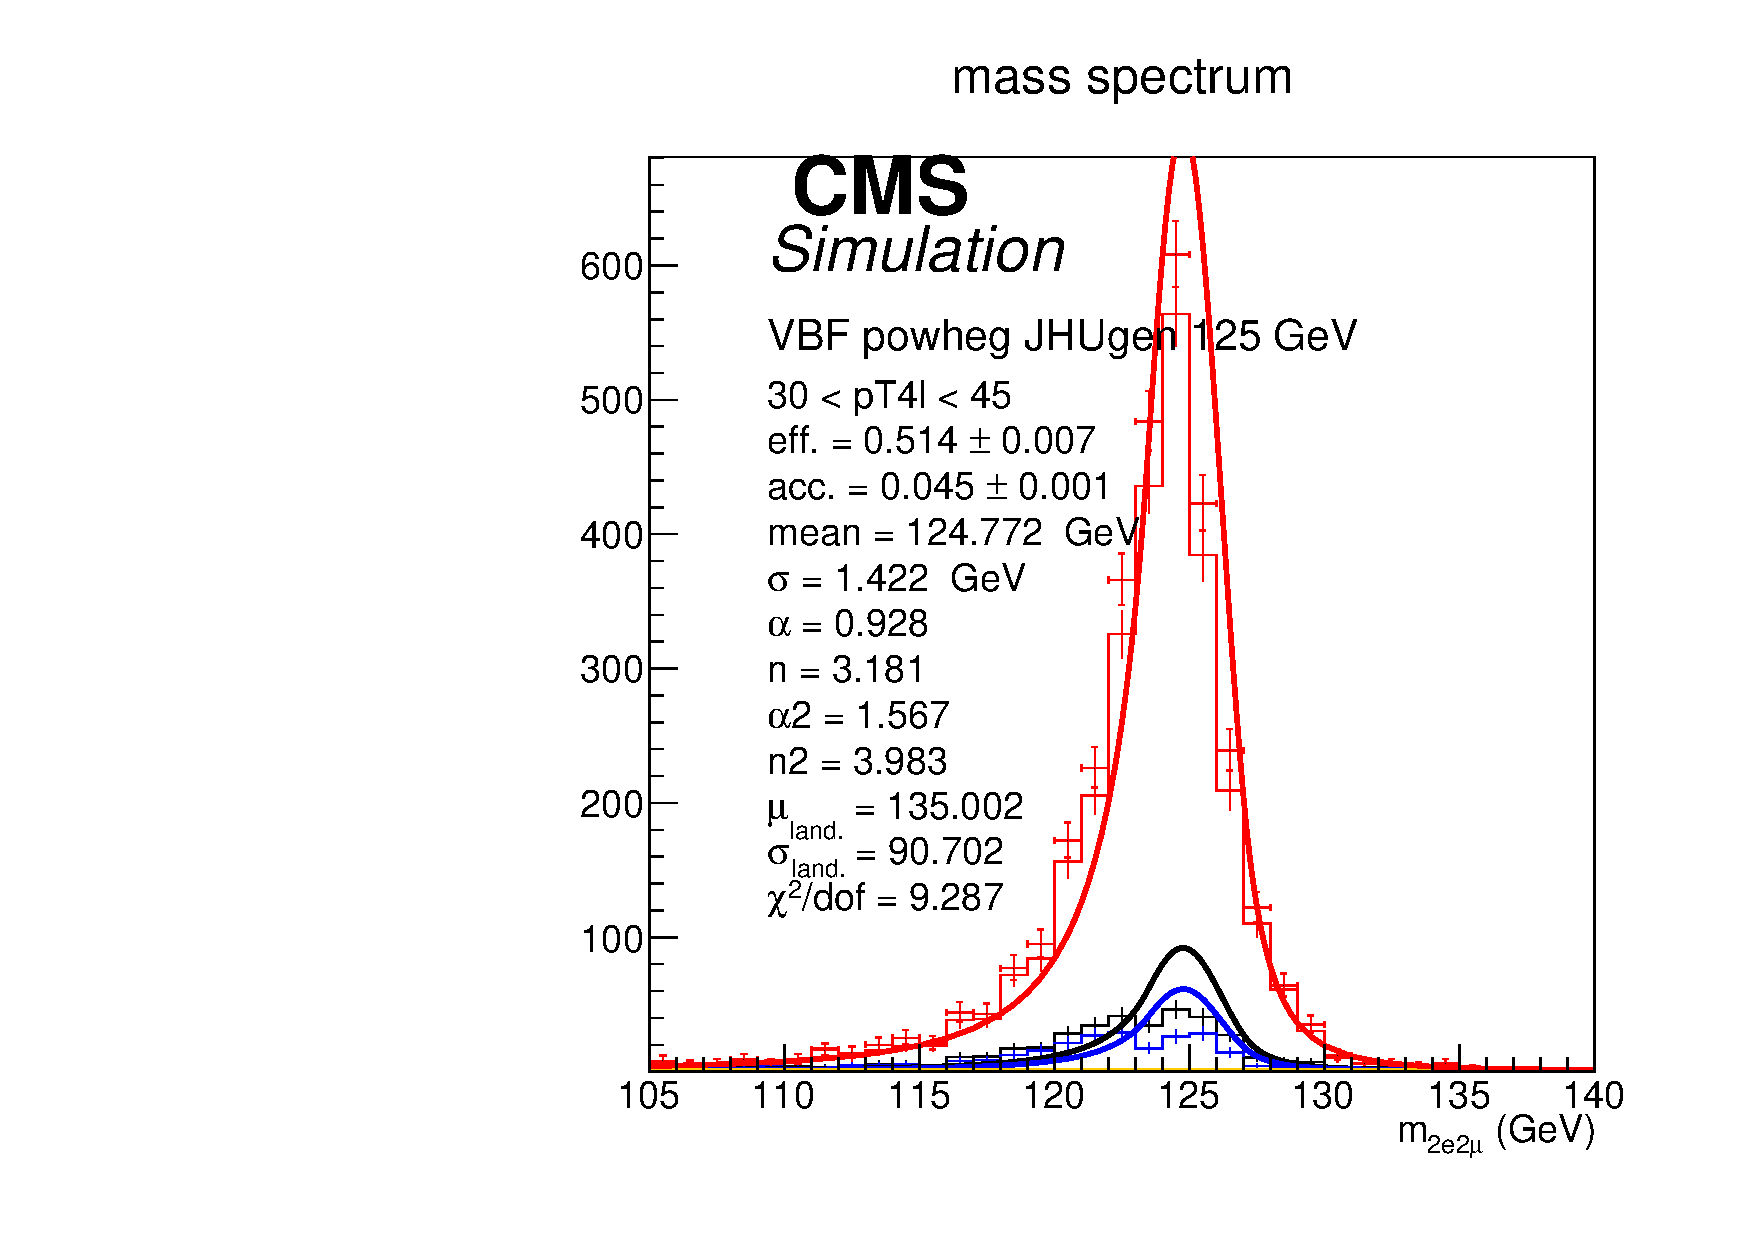
\includegraphics[width=0.3\textwidth,angle=0]{Figures/Appendix//VBF_powheg_JHUgen_125_2e2mu_pT4l_genbin2_recobin2_effs_genWeight*pileupWeight*dataMCWeight.pdf}
      \label{fig:sigfits-pT4l-VBF-powheg15-JHUgen-125-maintext:c}
    }  \\
    \subfigure[$45.0 < \pt(\mathrm{H}) < 80.0$]{
      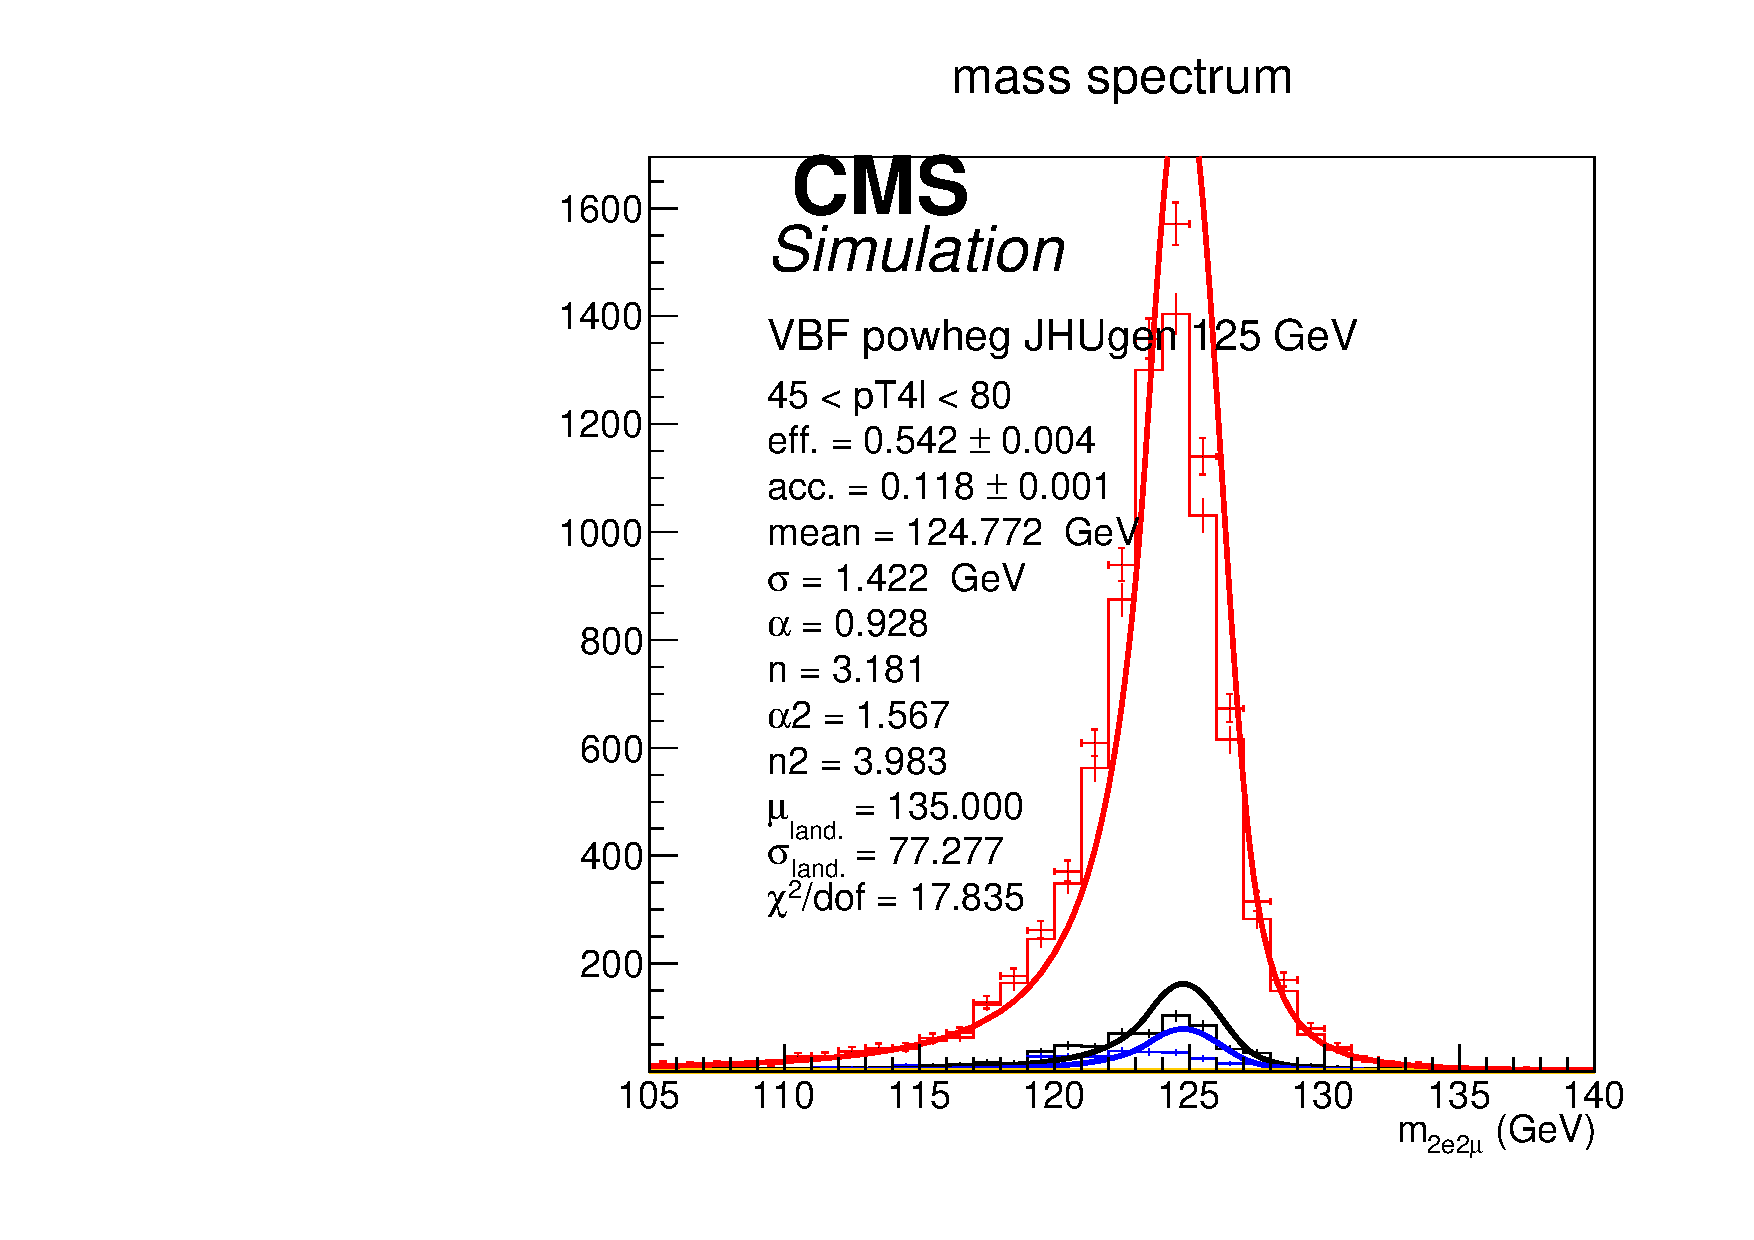
\includegraphics[width=0.3\textwidth,angle=0]{Figures/Appendix//VBF_powheg_JHUgen_125_2e2mu_pT4l_genbin3_recobin3_effs_genWeight*pileupWeight*dataMCWeight.pdf}
      \label{fig:sigfits-pT4l-VBF-powheg15-JHUgen-125-maintext:d}
    }
    \subfigure[$80.0 < \pt(\mathrm{H}) < 120.0$]{
      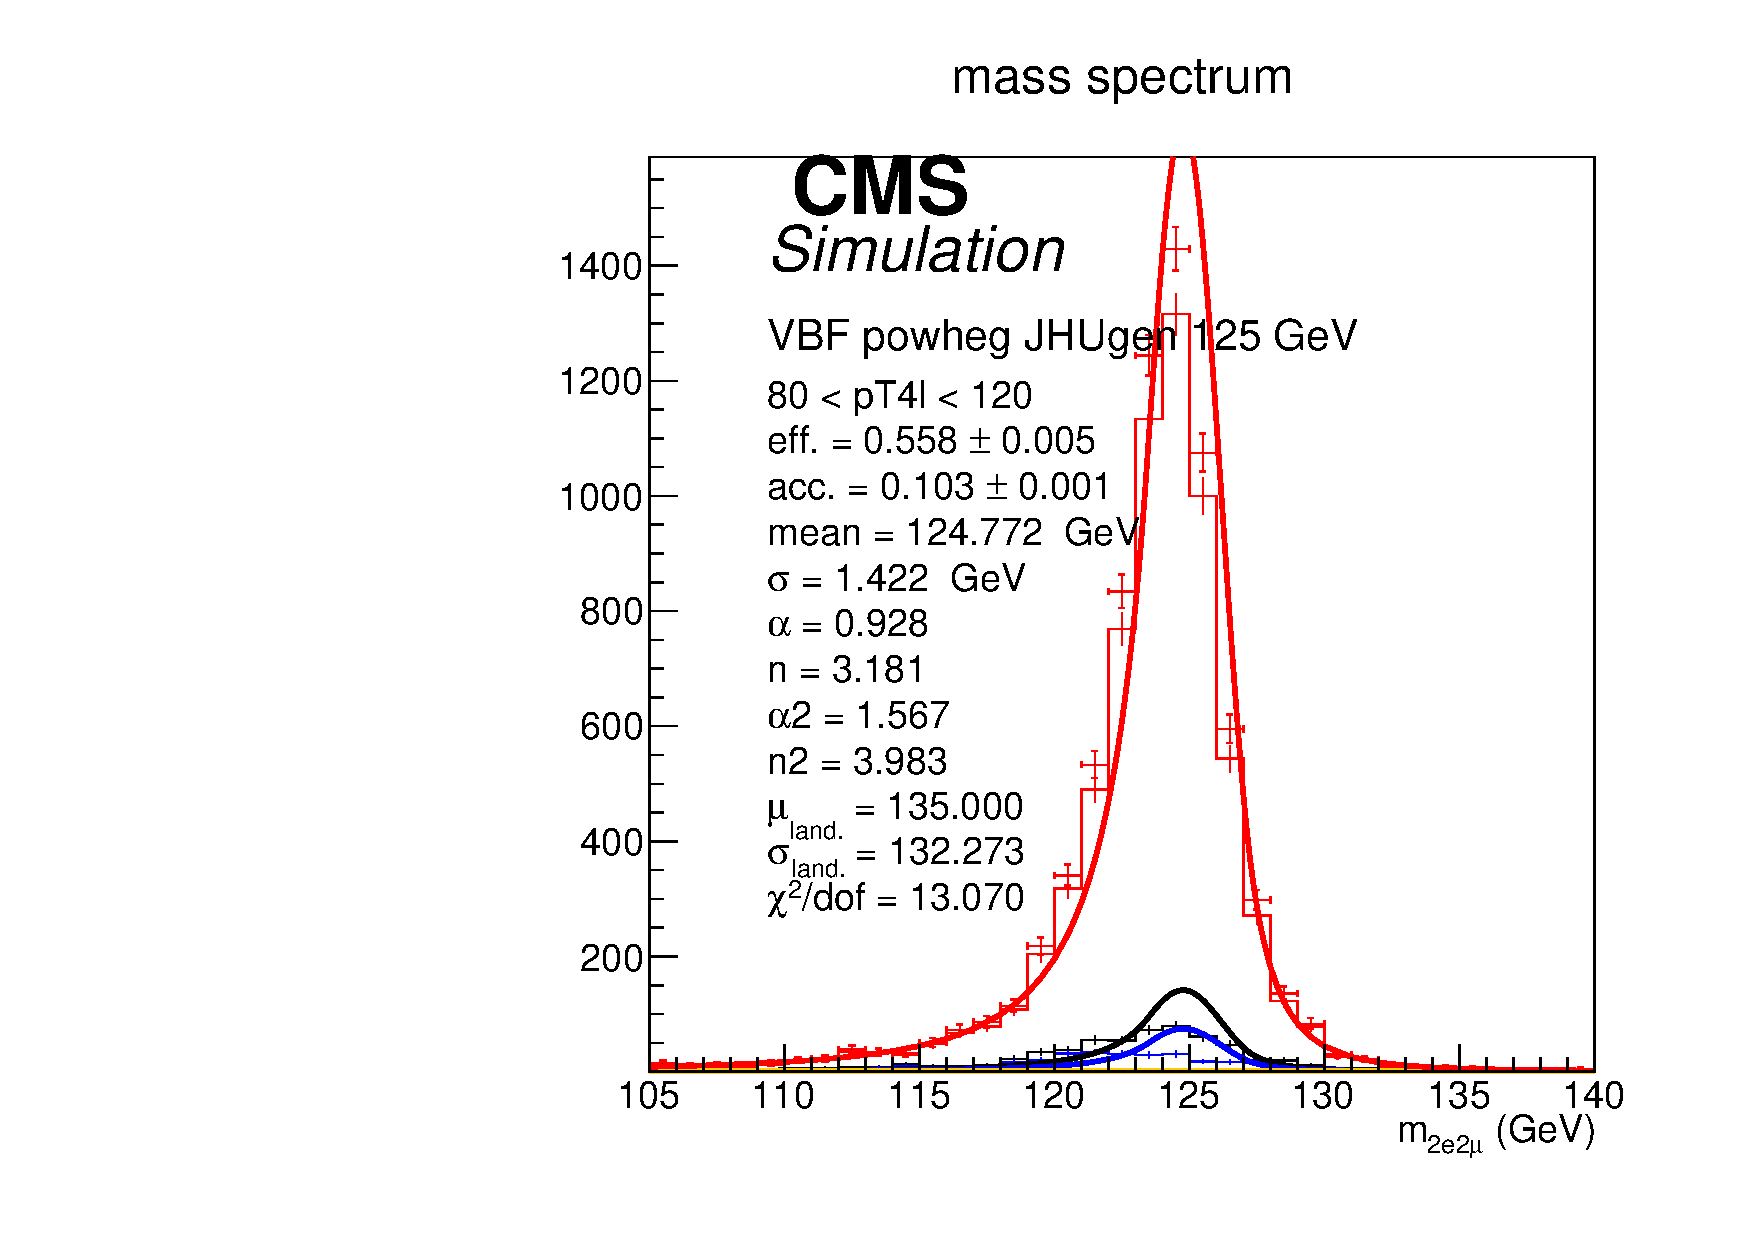
\includegraphics[width=0.3\textwidth,angle=0]{Figures/Appendix//VBF_powheg_JHUgen_125_2e2mu_pT4l_genbin4_recobin4_effs_genWeight*pileupWeight*dataMCWeight.pdf}
      \label{fig:sigfits-pT4l-VBF-powheg15-JHUgen-125-maintext:e}
    }
    \subfigure[$120.0 < \pt(\mathrm{H}) < 200.0$]{
      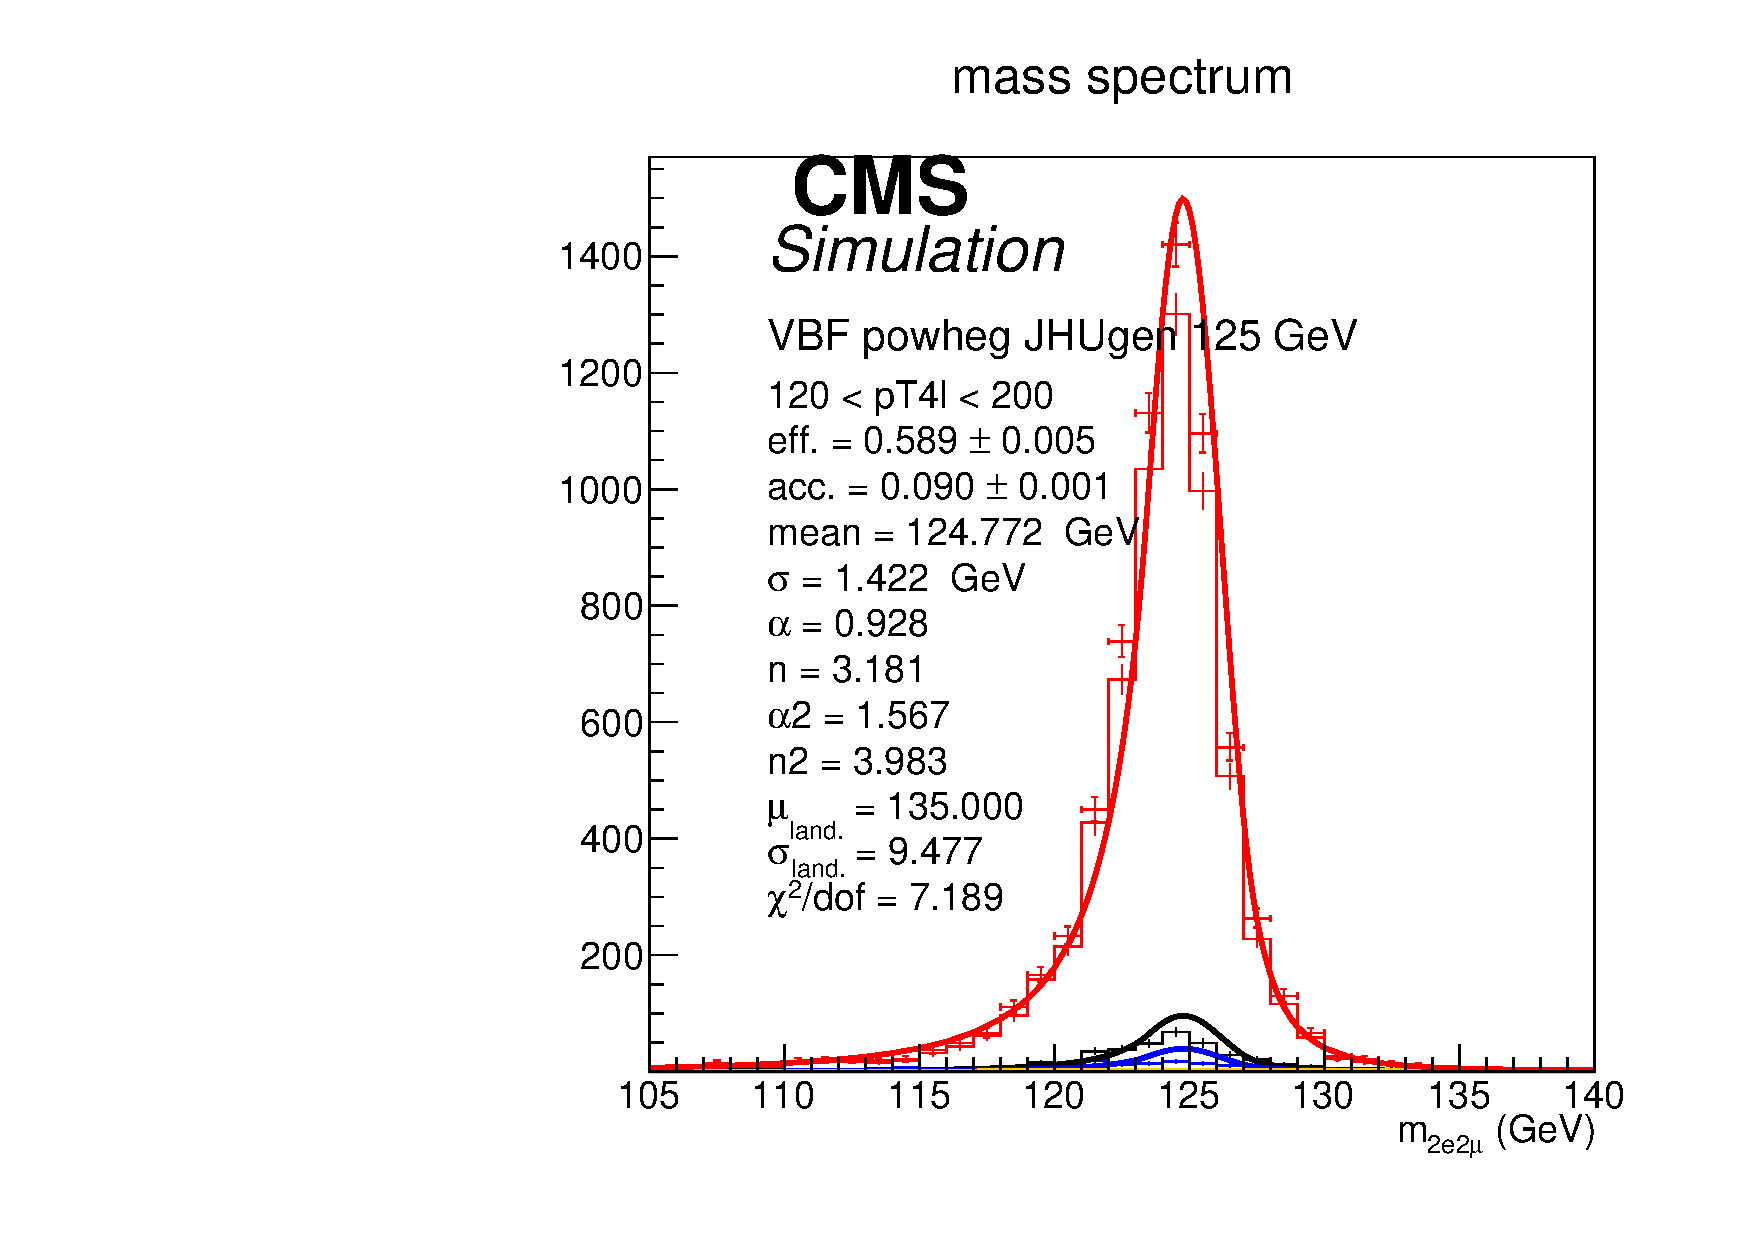
\includegraphics[width=0.3\textwidth,angle=0]{Figures/Appendix//VBF_powheg_JHUgen_125_2e2mu_pT4l_genbin5_recobin5_effs_genWeight*pileupWeight*dataMCWeight.pdf}
      \label{fig:sigfits-pT4l-VBF-powheg15-JHUgen-125-maintext:f}
    } \\
    \subfigure[$200.0 < \pt(\mathrm{H}) < 13000.0$]{
      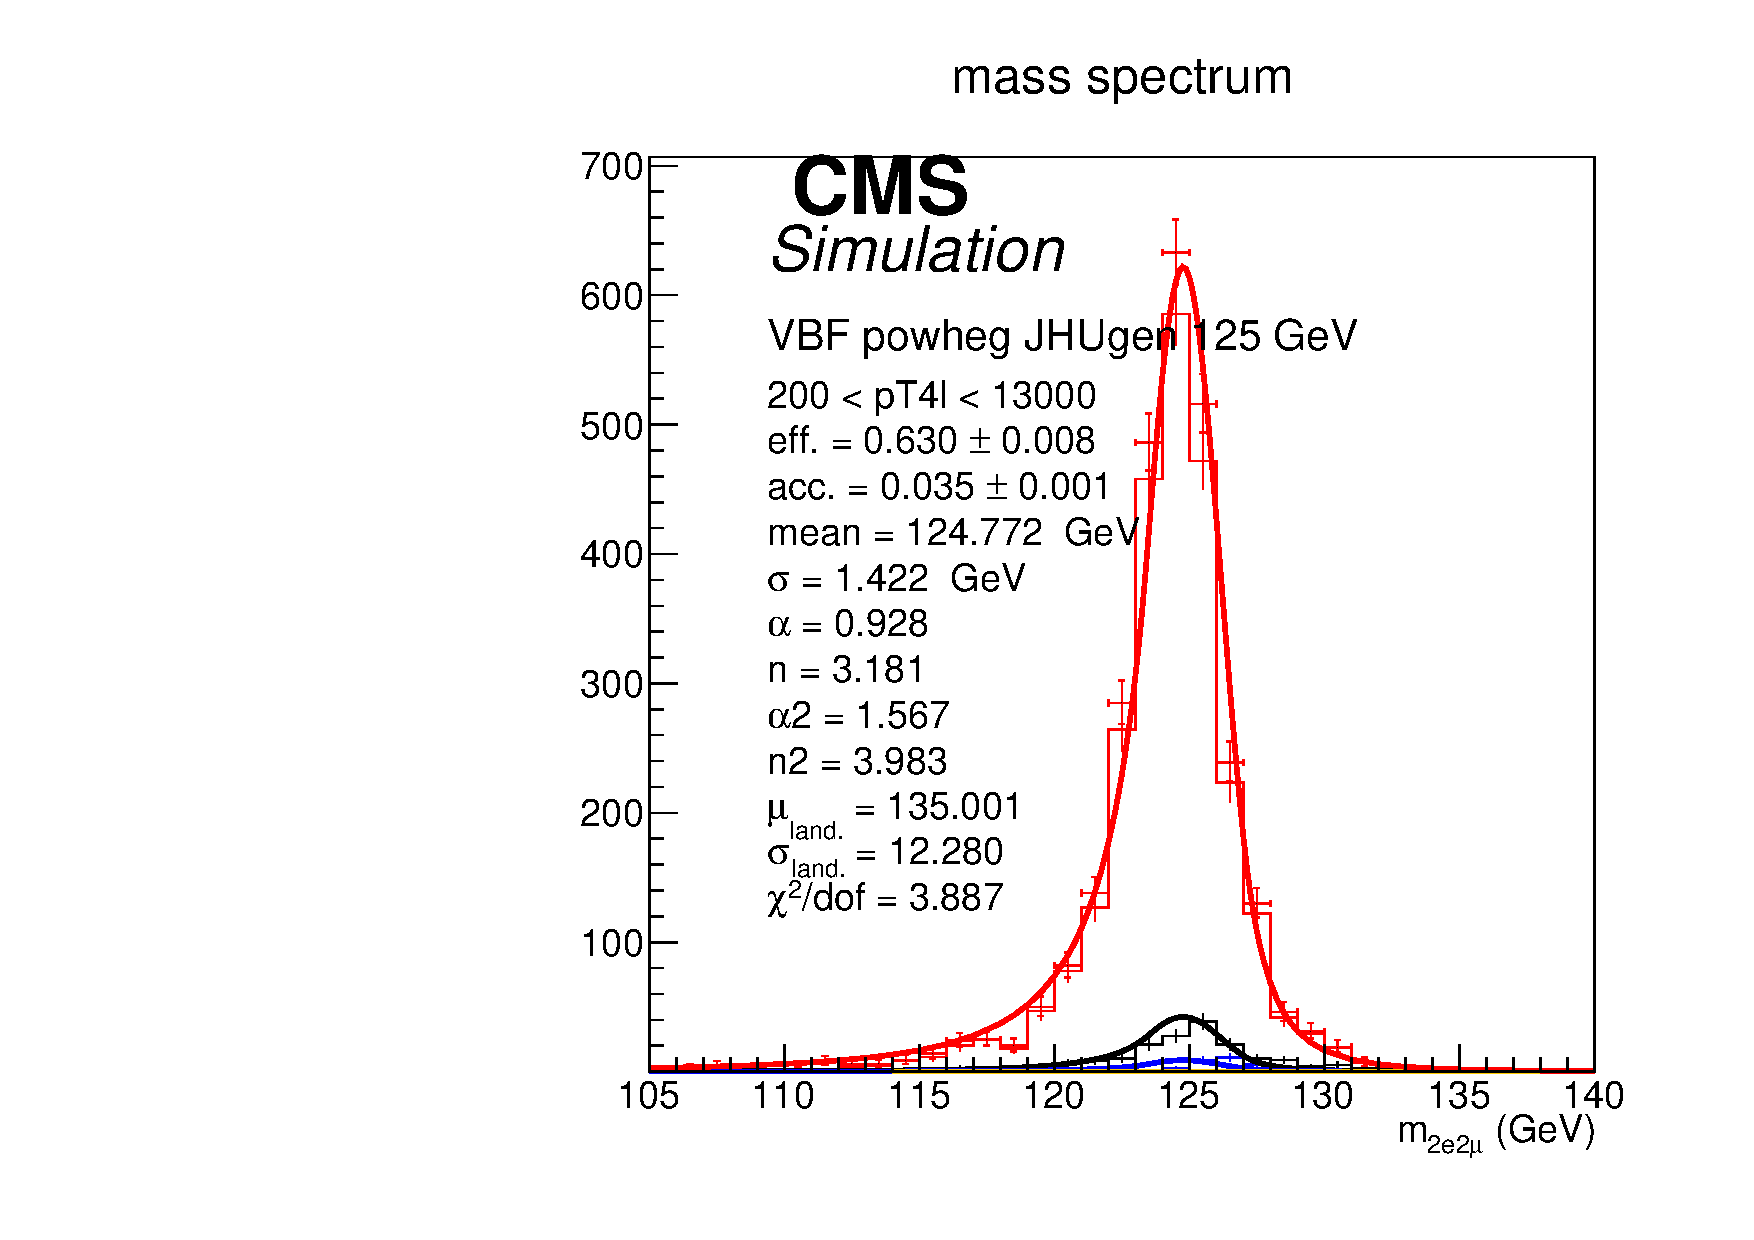
\includegraphics[width=0.3\textwidth,angle=0]{Figures/Appendix//VBF_powheg_JHUgen_125_2e2mu_pT4l_genbin6_recobin6_effs_genWeight*pileupWeight*dataMCWeight.pdf}
      \label{fig:sigfits-pT4l-VBF-powheg15-JHUgen-125-maintext:g}
    }
    \\
    \caption{ Example signal shapes at reconstruction level for a resonance of m(4$\ell$) in $2e2\mu$ final state for the $VBF$ production mode from {\sc powheg+JHUGen} in different bins of $\pt(\mathrm{H})$. The black curve represents events which do not pass the fiducial volume selection. The curve has no effect on the result.
    }
  \label{fig:sigfits-pT4l-VBF-powheg15-JHUgen-125-maintext}
 \end{center}
\end{figure} \clearpage

\begin{figure}[htb]
  \begin{center}
    \subfigure[$0.0 < \pt(\mathrm{H}) < 15.0 $]{
      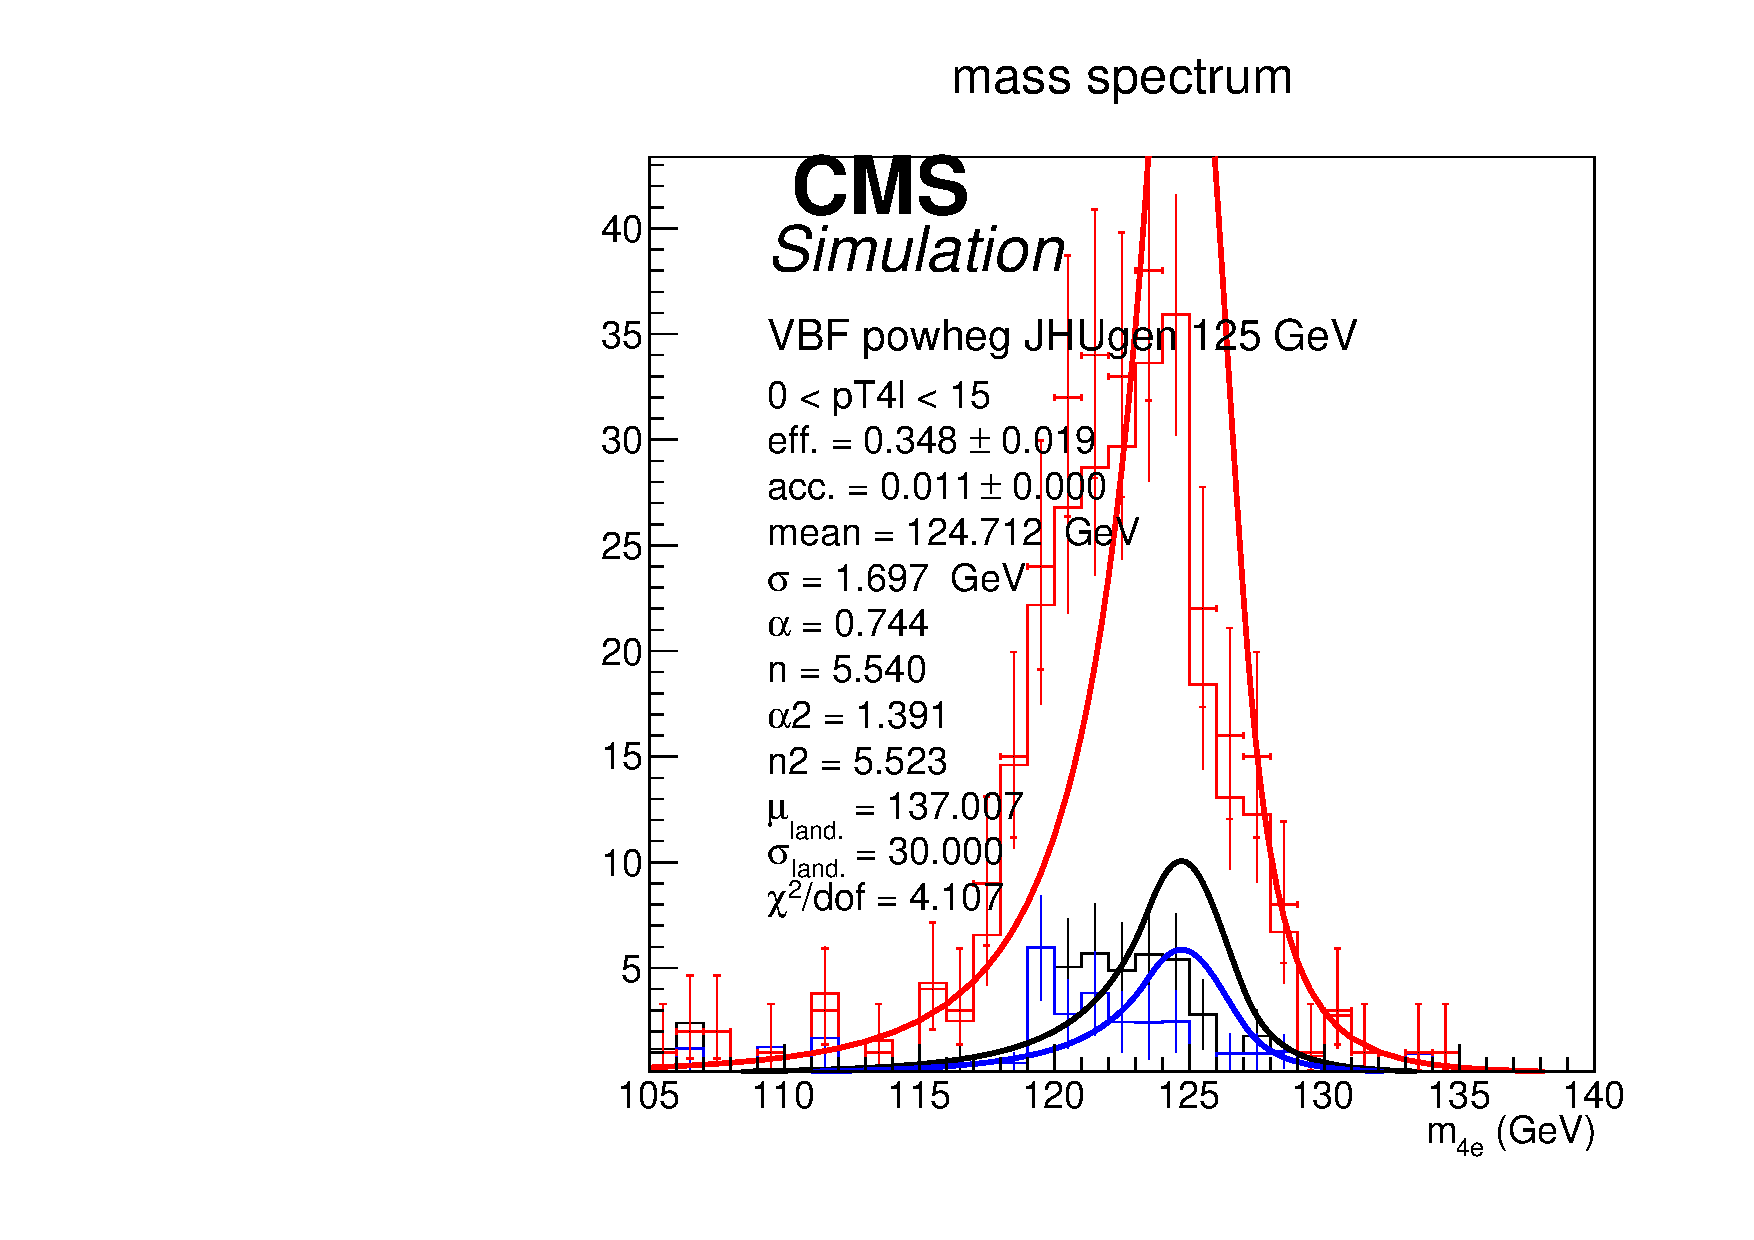
\includegraphics[width=0.3\textwidth,angle=0]{Figures/Appendix//VBF_powheg_JHUgen_125_4e_pT4l_genbin0_recobin0_effs_genWeight*pileupWeight*dataMCWeight.pdf}
      \label{fig:sigfits-pT4l-VBF-powheg15-JHUgen-125-maintext:a}
    }
    \subfigure[$15.0 < \pt(\mathrm{H}) < 30.0$]{
      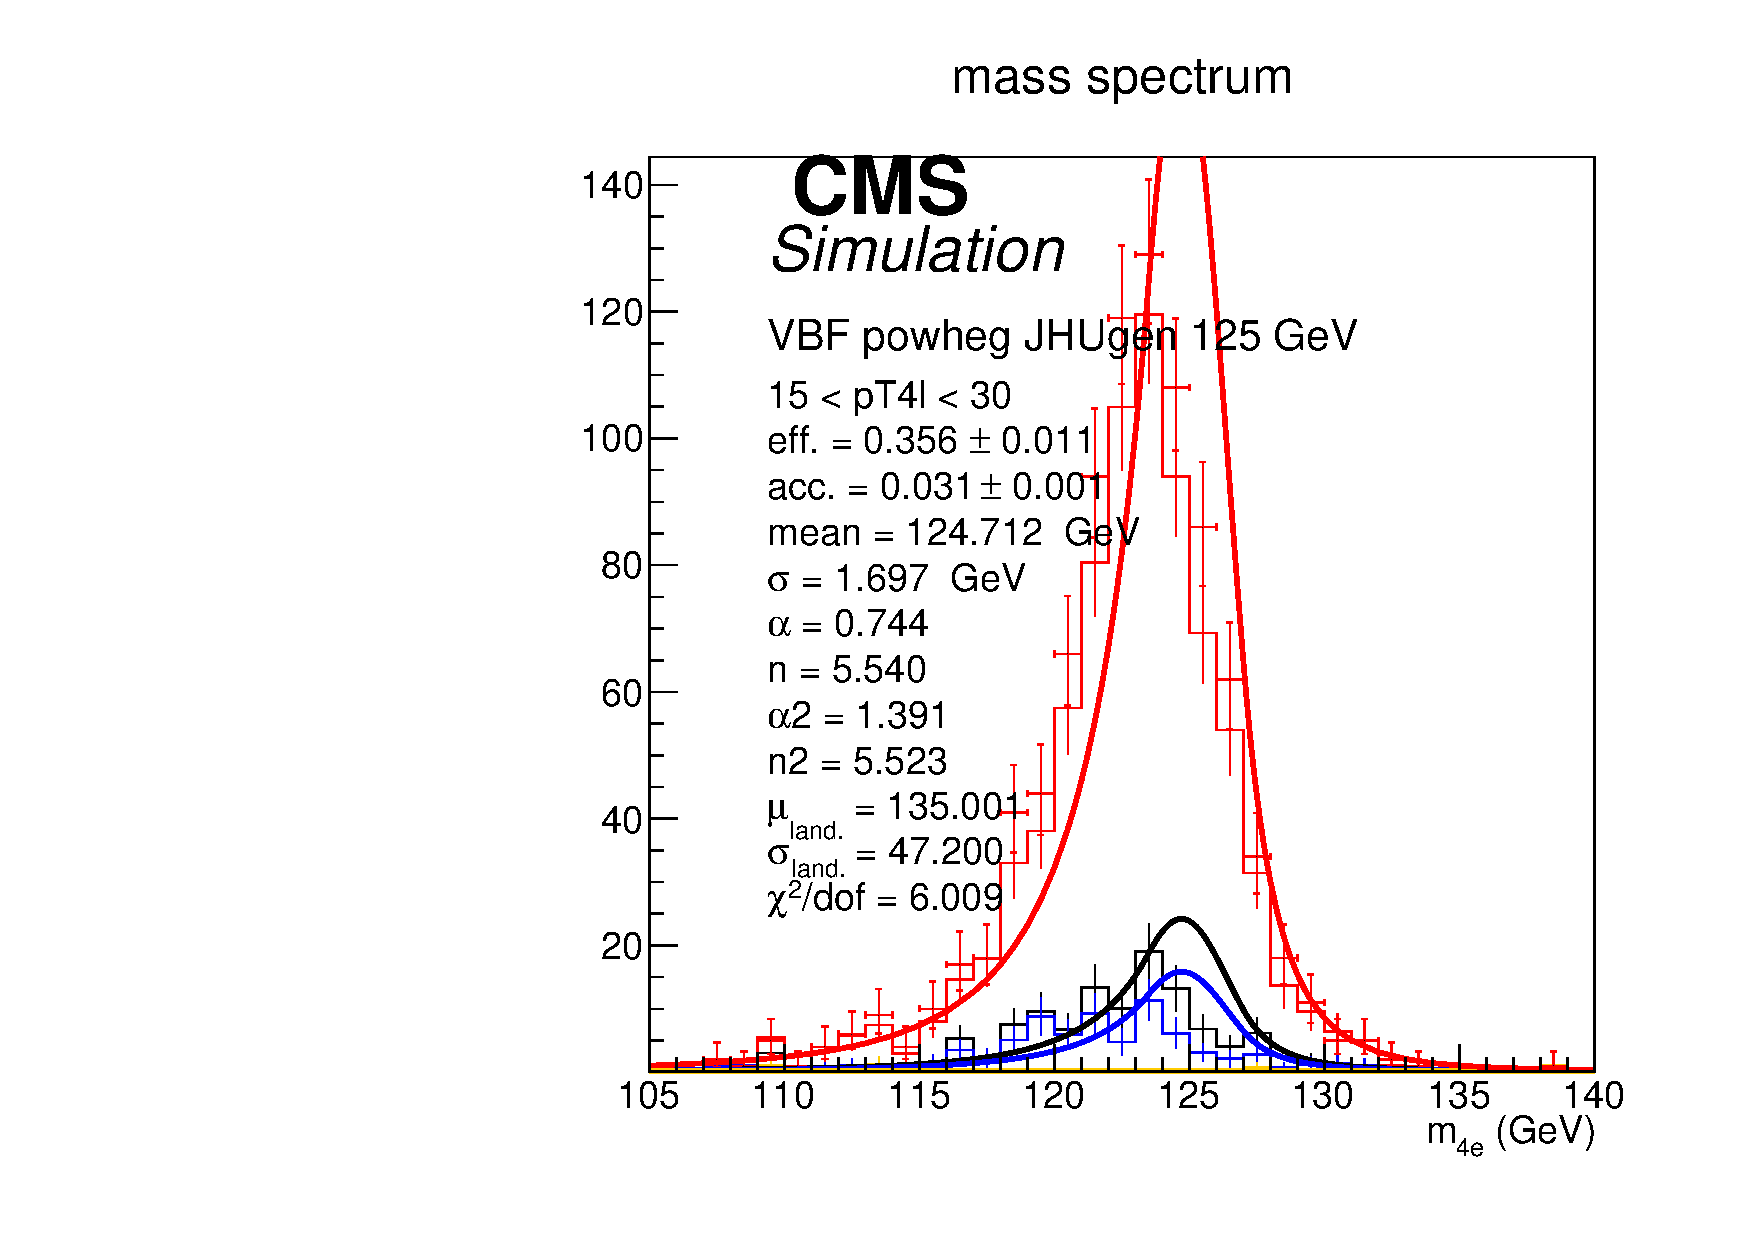
\includegraphics[width=0.3\textwidth,angle=0]{Figures/Appendix//VBF_powheg_JHUgen_125_4e_pT4l_genbin1_recobin1_effs_genWeight*pileupWeight*dataMCWeight.pdf}
      \label{fig:sigfits-pT4l-VBF-powheg15-JHUgen-125-maintext:b}
    }
   \subfigure[$30.0 < \pt(\mathrm{H}) < 45.0$]{
      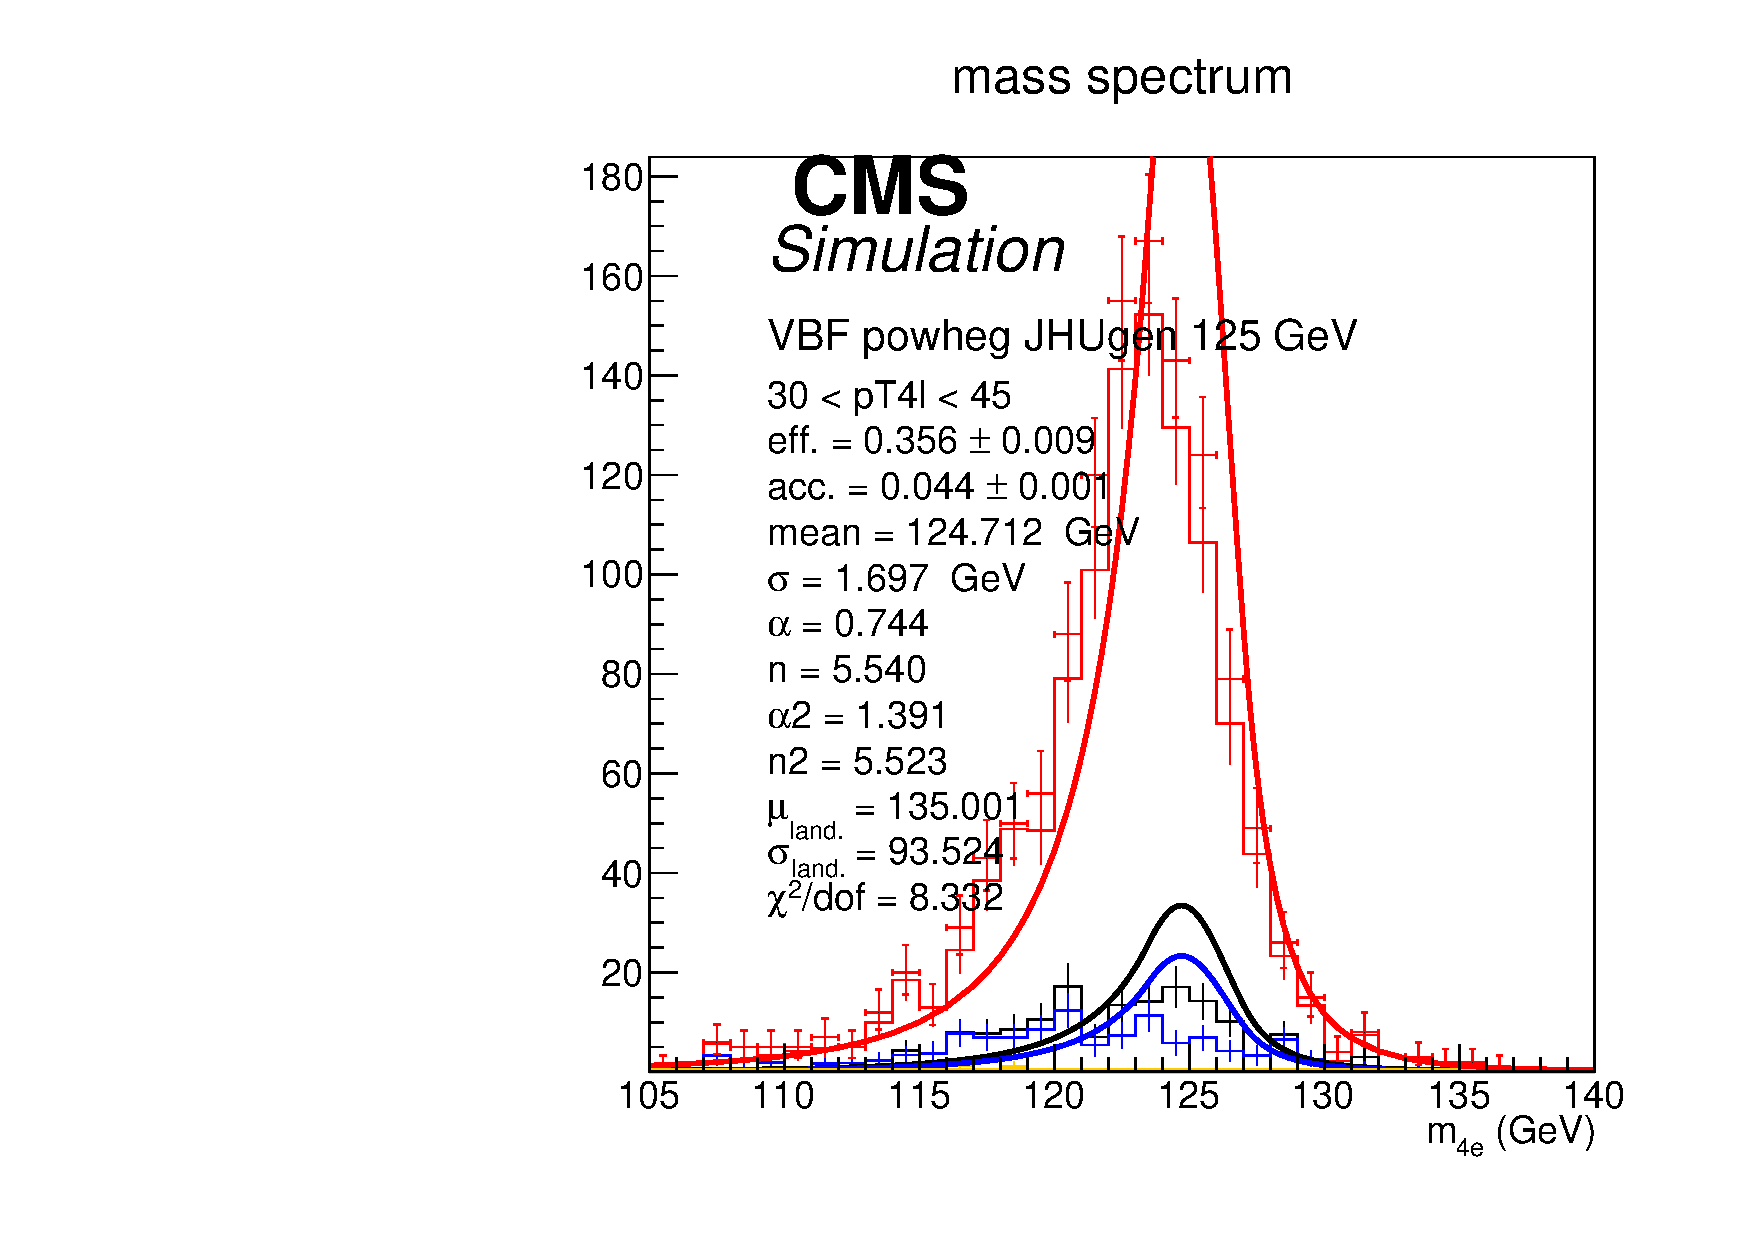
\includegraphics[width=0.3\textwidth,angle=0]{Figures/Appendix//VBF_powheg_JHUgen_125_4e_pT4l_genbin2_recobin2_effs_genWeight*pileupWeight*dataMCWeight.pdf}
      \label{fig:sigfits-pT4l-VBF-powheg15-JHUgen-125-maintext:c}
    }  \\
    \subfigure[$45.0 < \pt(\mathrm{H}) < 80.0$]{
      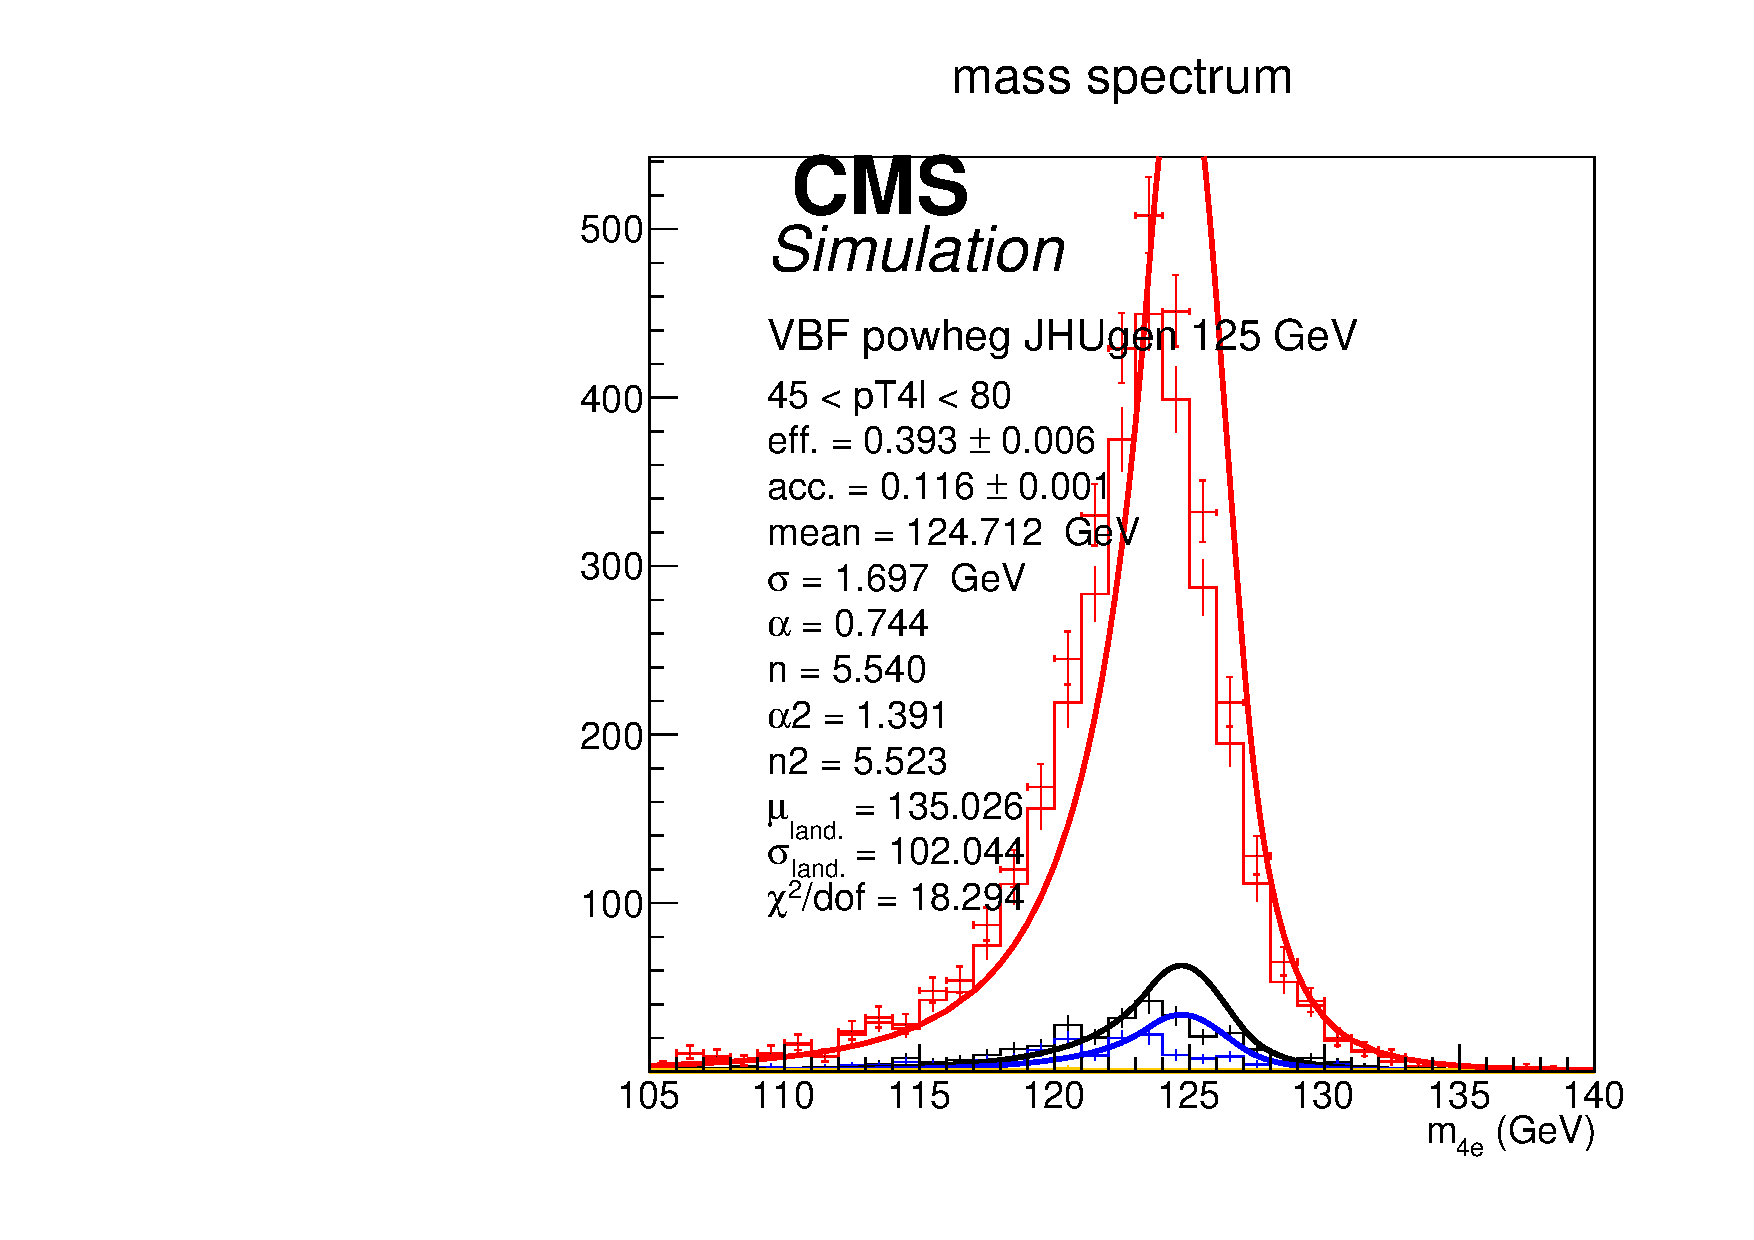
\includegraphics[width=0.3\textwidth,angle=0]{Figures/Appendix//VBF_powheg_JHUgen_125_4e_pT4l_genbin3_recobin3_effs_genWeight*pileupWeight*dataMCWeight.pdf}
      \label{fig:sigfits-pT4l-VBF-powheg15-JHUgen-125-maintext:d}
    }
    \subfigure[$80.0 < \pt(\mathrm{H}) < 120.0$]{
      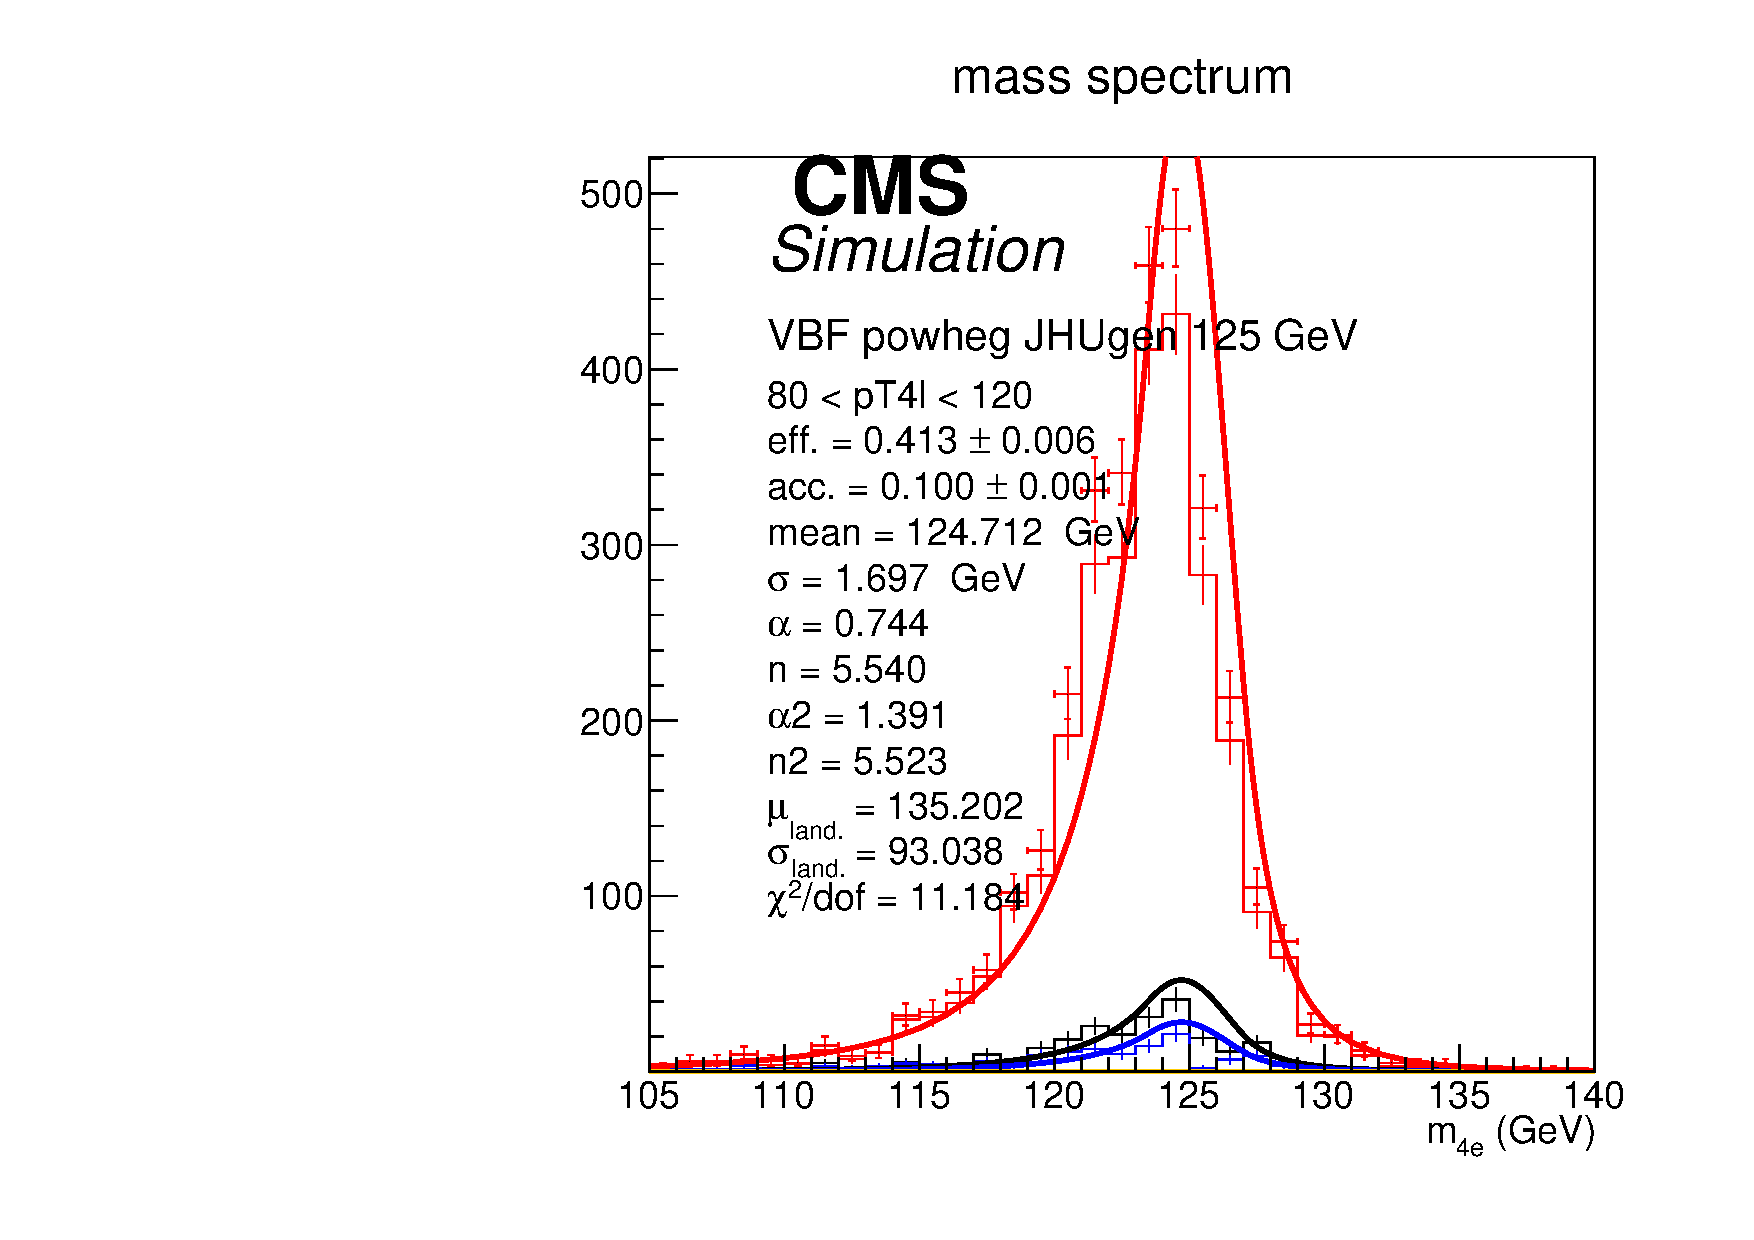
\includegraphics[width=0.3\textwidth,angle=0]{Figures/Appendix//VBF_powheg_JHUgen_125_4e_pT4l_genbin4_recobin4_effs_genWeight*pileupWeight*dataMCWeight.pdf}
      \label{fig:sigfits-pT4l-VBF-powheg15-JHUgen-125-maintext:e}
    }
    \subfigure[$120.0 < \pt(\mathrm{H}) < 200.0$]{
      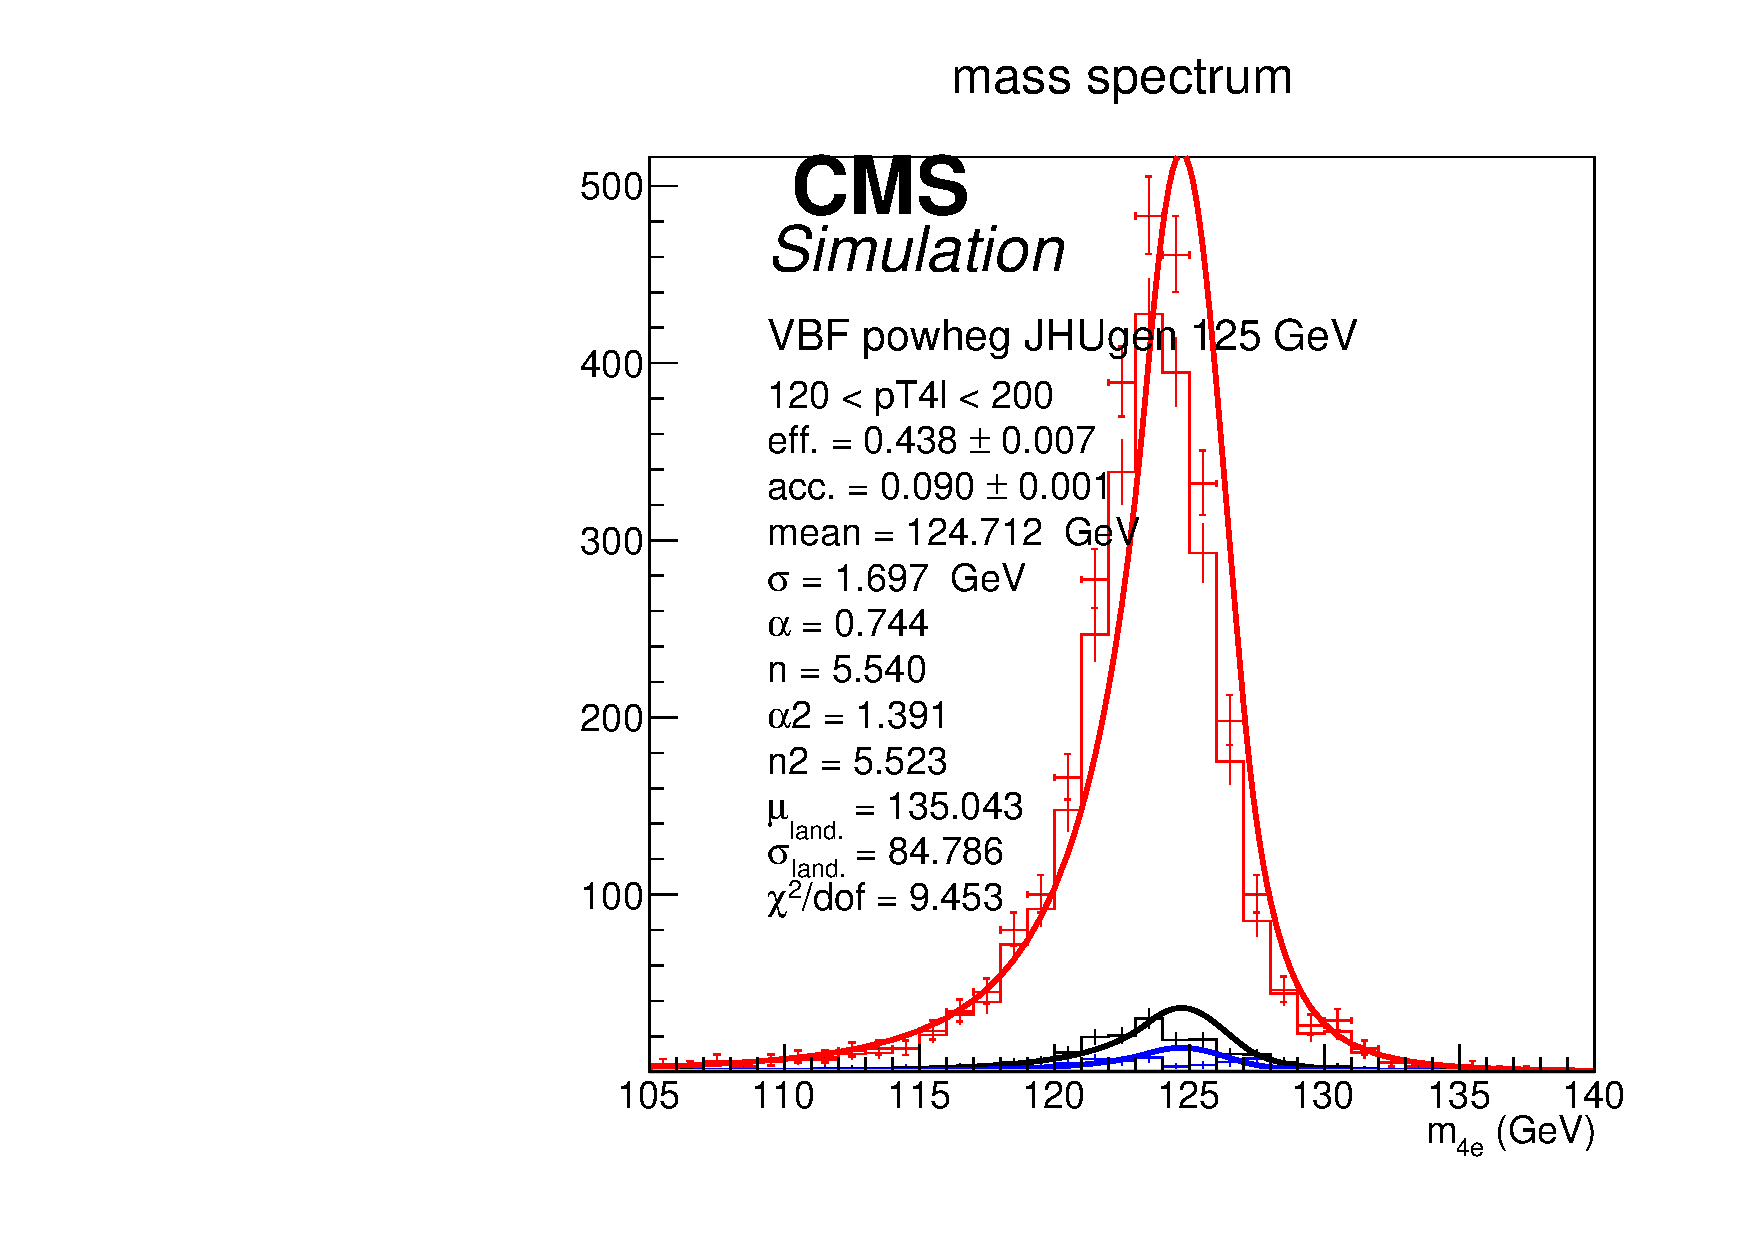
\includegraphics[width=0.3\textwidth,angle=0]{Figures/Appendix//VBF_powheg_JHUgen_125_4e_pT4l_genbin5_recobin5_effs_genWeight*pileupWeight*dataMCWeight.pdf}
      \label{fig:sigfits-pT4l-VBF-powheg15-JHUgen-125-maintext:f}
    } \\
    \subfigure[$200.0 < \pt(\mathrm{H}) < 13000.0$]{
      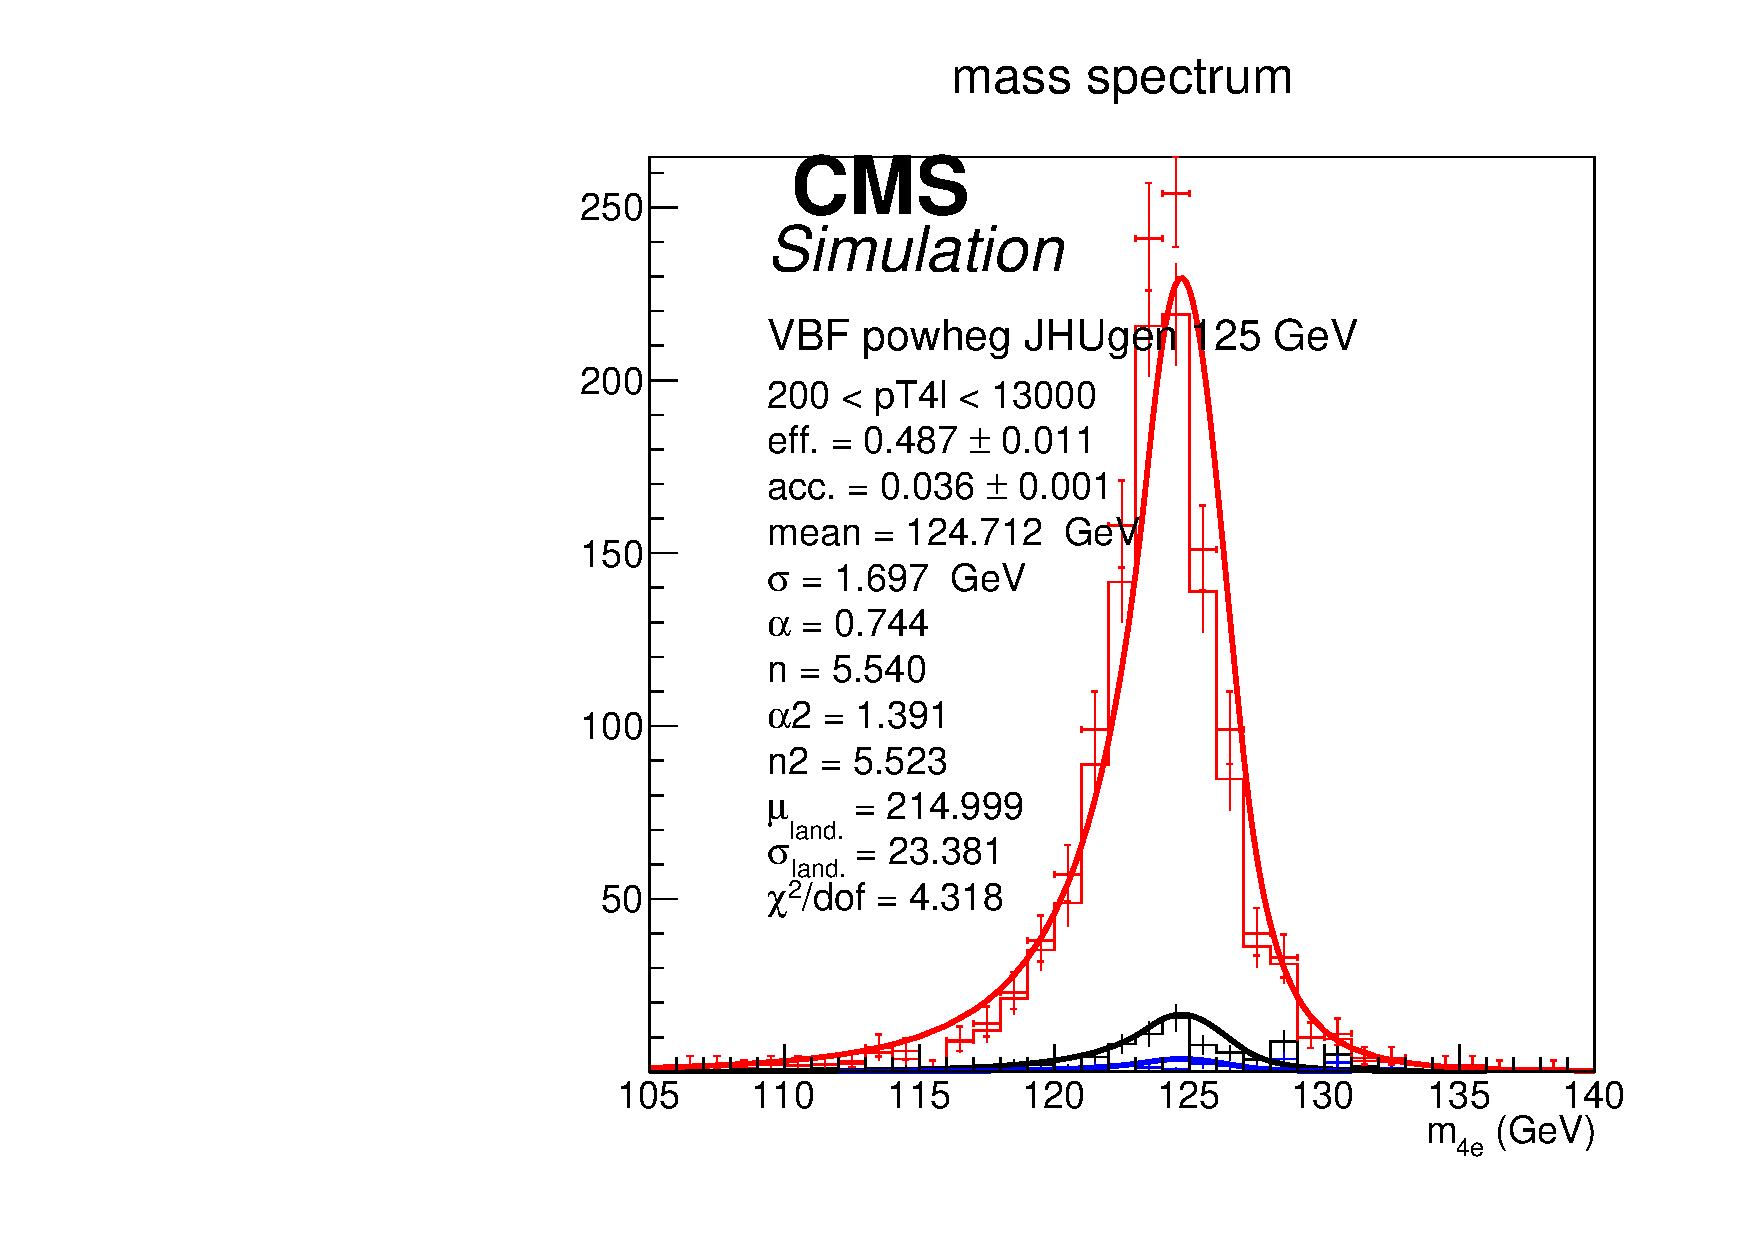
\includegraphics[width=0.3\textwidth,angle=0]{Figures/Appendix//VBF_powheg_JHUgen_125_4e_pT4l_genbin6_recobin6_effs_genWeight*pileupWeight*dataMCWeight.pdf}
      \label{fig:sigfits-pT4l-VBF-powheg15-JHUgen-125-maintext:g}
    }
    \\
    \caption{ Example signal shapes at reconstruction level for a resonance of m(4$\ell$) in $4e$ final state for the $VBF$ production mode from {\sc powheg+JHUGen} in different bins of $\pt(\mathrm{H})$. The black curve represents events which do not pass the fiducial volume selection. The curve has no effect on the result.
    }
  \label{fig:sigfits-pT4l-VBF-powheg15-JHUgen-125-maintext}
 \end{center}
\end{figure} \clearpage


\begin{figure}[htb]
  \begin{center}
    \subfigure[$0.0 < \pt(\mathrm{H}) < 15.0 $]{
      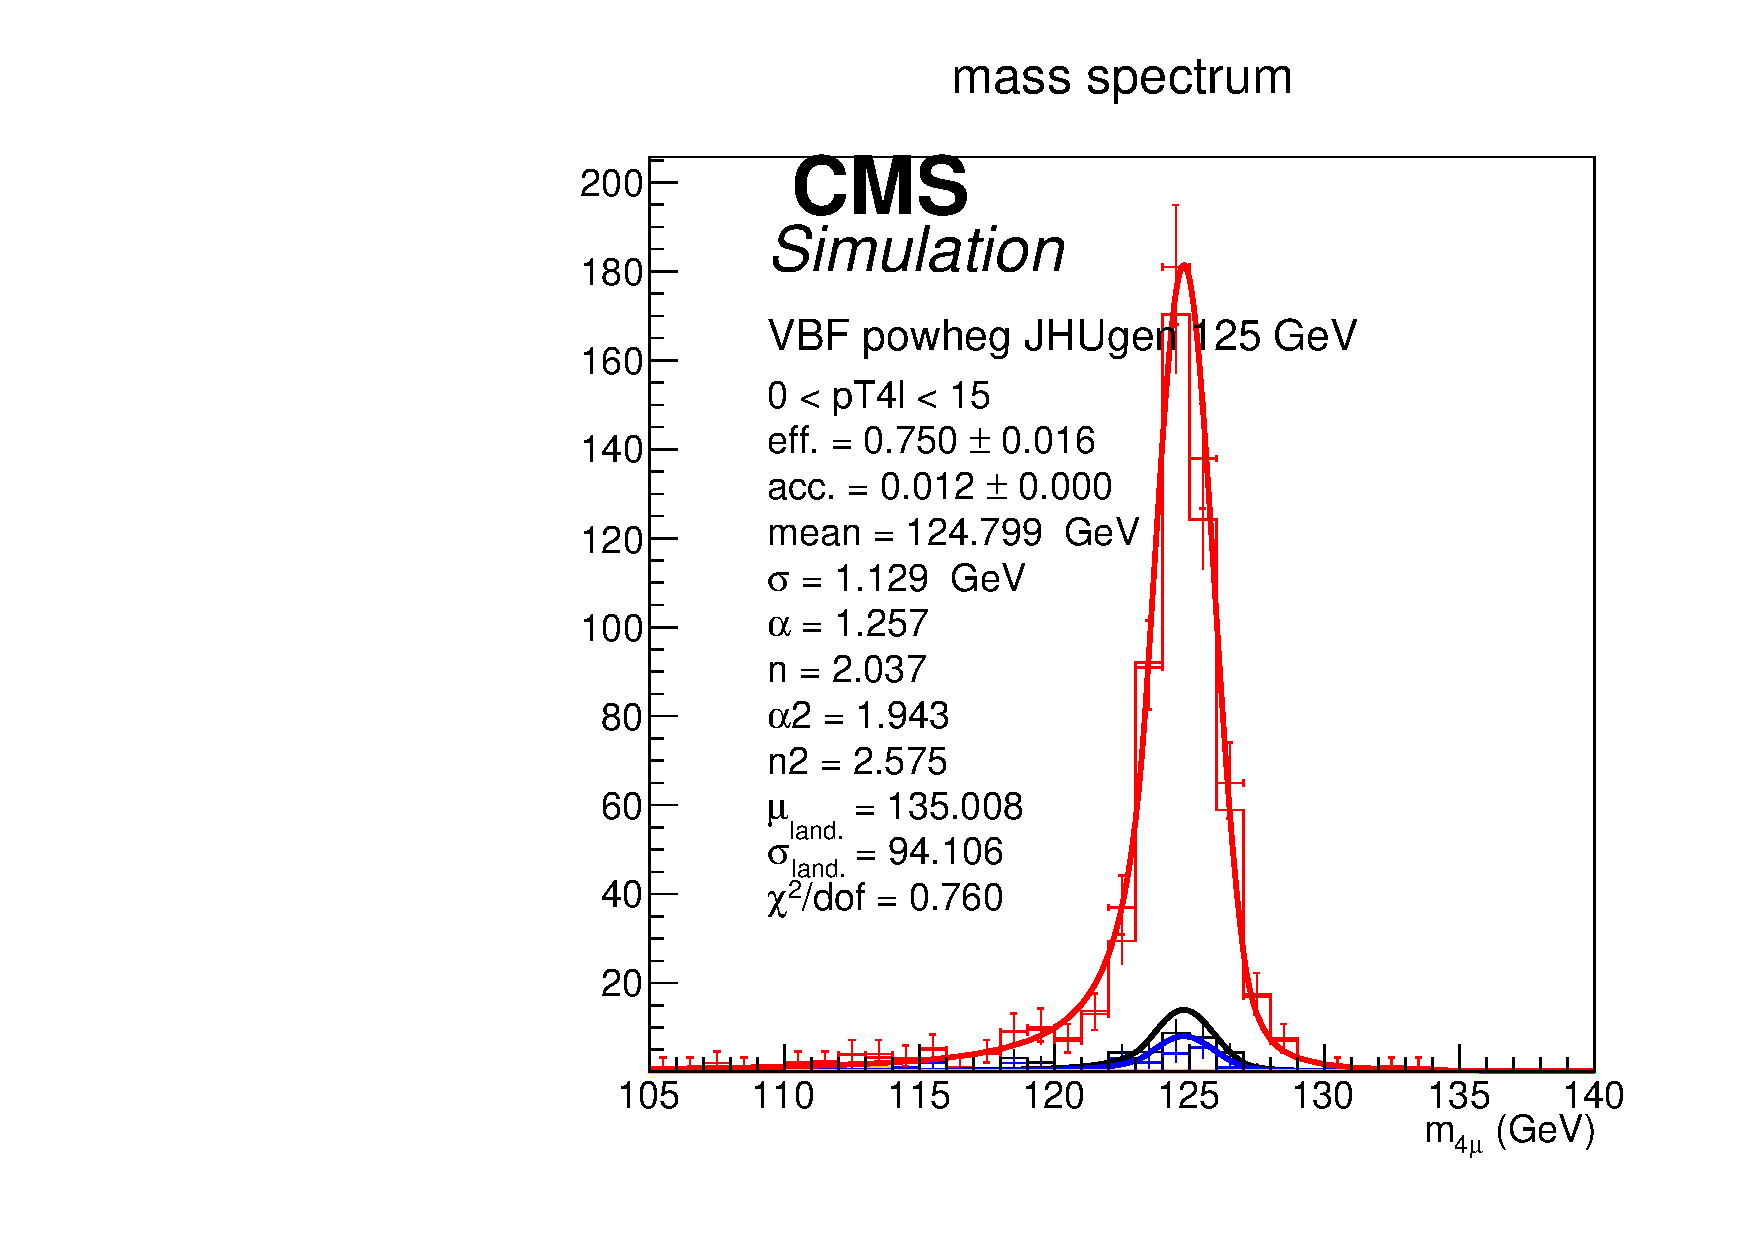
\includegraphics[width=0.3\textwidth,angle=0]{Figures/Appendix//VBF_powheg_JHUgen_125_4mu_pT4l_genbin0_recobin0_effs_genWeight*pileupWeight*dataMCWeight.pdf}
      \label{fig:sigfits-pT4l-VBF-powheg15-JHUgen-125-maintext:a}
    }
    \subfigure[$15.0 < \pt(\mathrm{H}) < 30.0$]{
      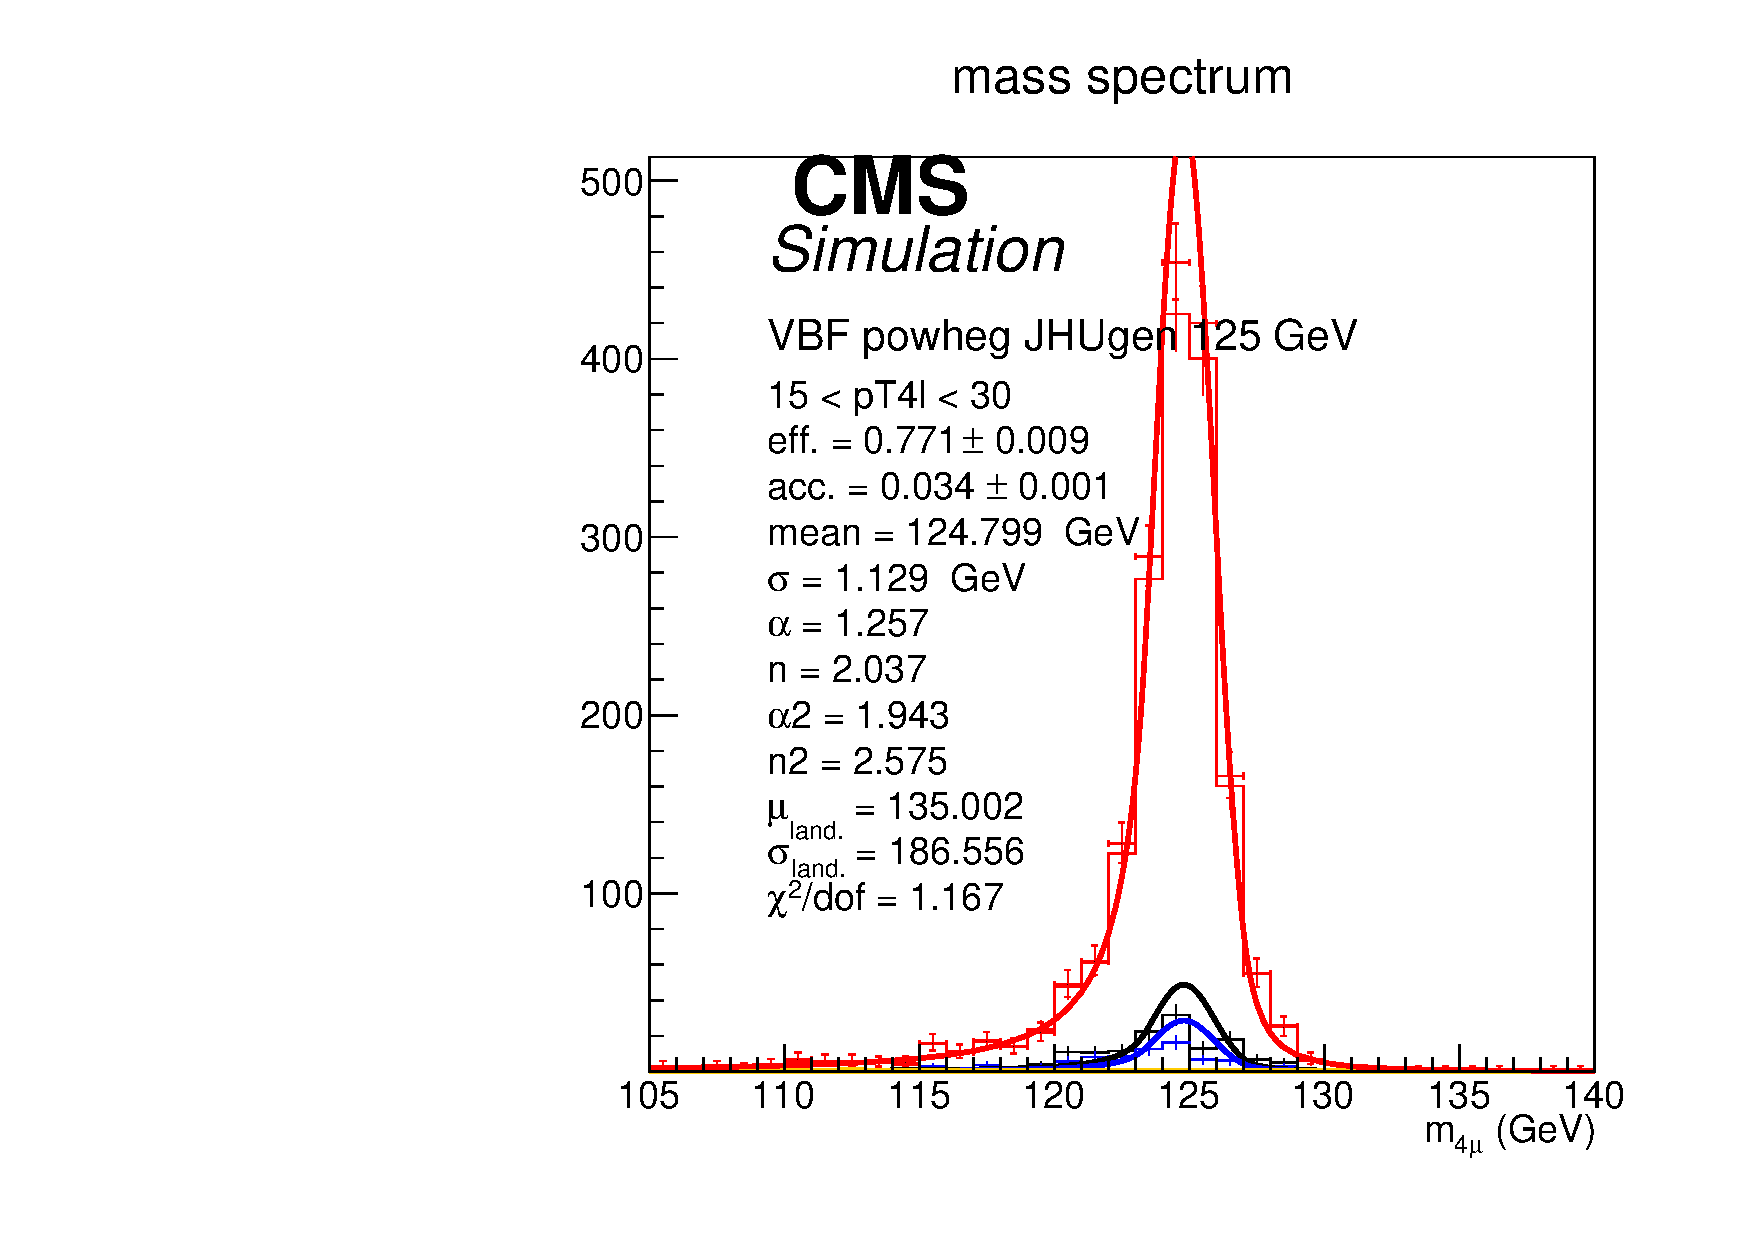
\includegraphics[width=0.3\textwidth,angle=0]{Figures/Appendix//VBF_powheg_JHUgen_125_4mu_pT4l_genbin1_recobin1_effs_genWeight*pileupWeight*dataMCWeight.pdf}
      \label{fig:sigfits-pT4l-VBF-powheg15-JHUgen-125-maintext:b}
    }
   \subfigure[$30.0 < \pt(\mathrm{H}) < 45.0$]{
      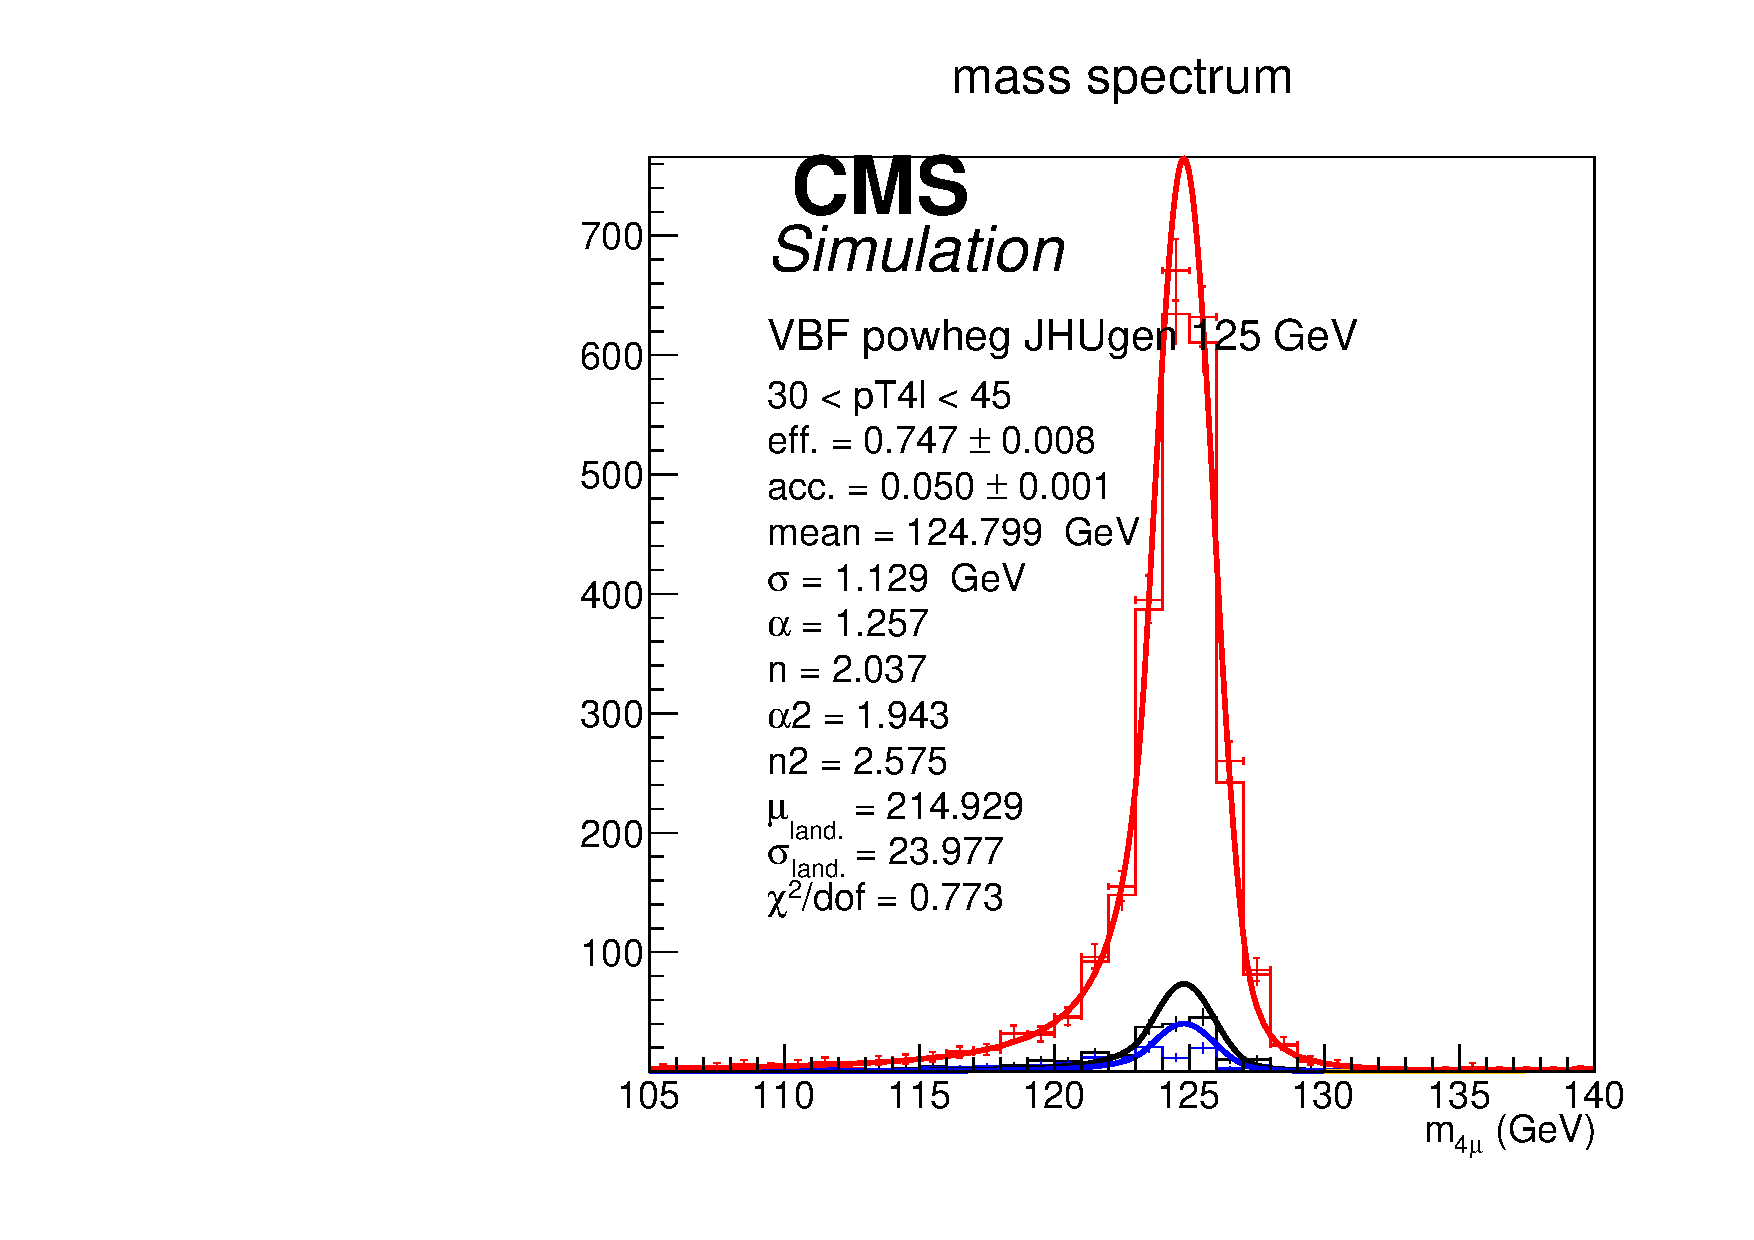
\includegraphics[width=0.3\textwidth,angle=0]{Figures/Appendix//VBF_powheg_JHUgen_125_4mu_pT4l_genbin2_recobin2_effs_genWeight*pileupWeight*dataMCWeight.pdf}
      \label{fig:sigfits-pT4l-VBF-powheg15-JHUgen-125-maintext:c}
    }  \\
    \subfigure[$45.0 < \pt(\mathrm{H}) < 80.0$]{
      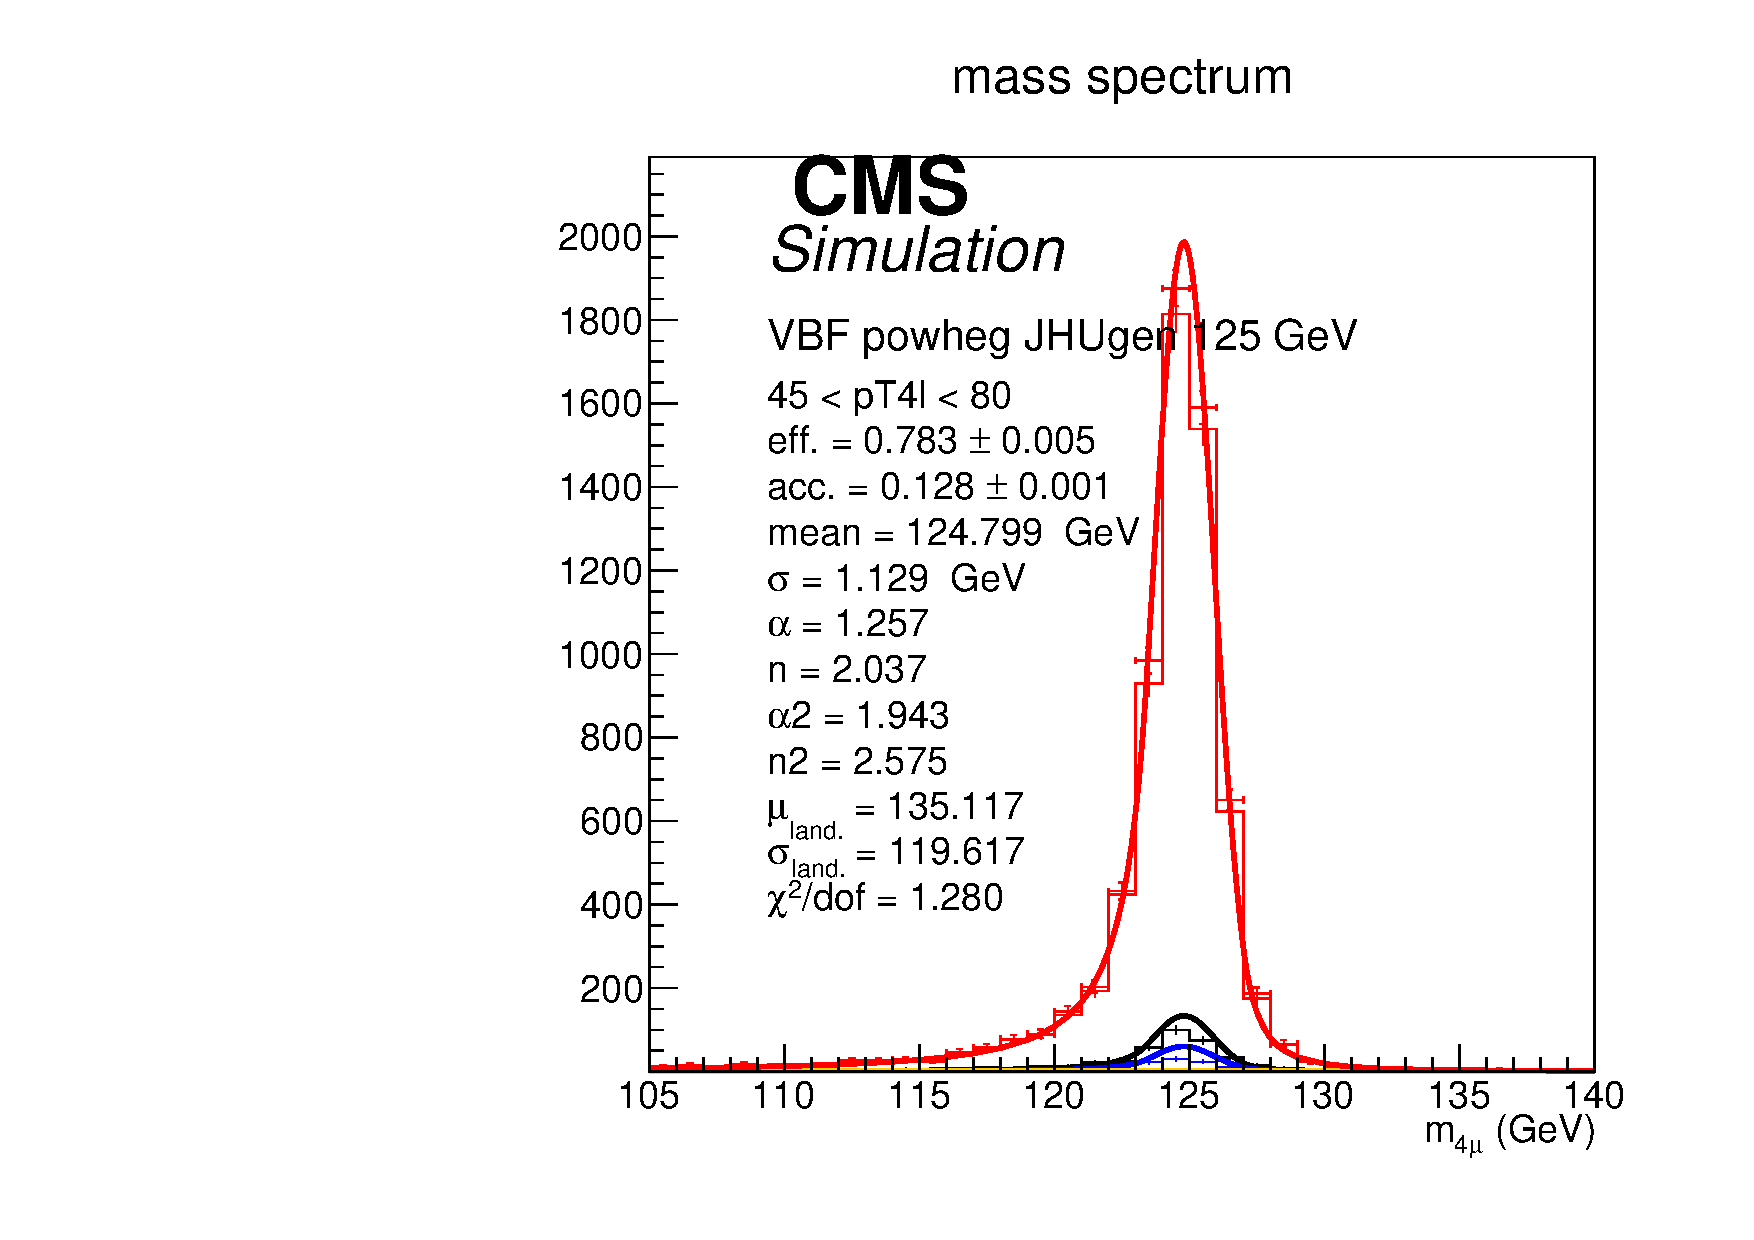
\includegraphics[width=0.3\textwidth,angle=0]{Figures/Appendix//VBF_powheg_JHUgen_125_4mu_pT4l_genbin3_recobin3_effs_genWeight*pileupWeight*dataMCWeight.pdf}
      \label{fig:sigfits-pT4l-VBF-powheg15-JHUgen-125-maintext:d}
    }
    \subfigure[$80.0 < \pt(\mathrm{H}) < 120.0$]{
      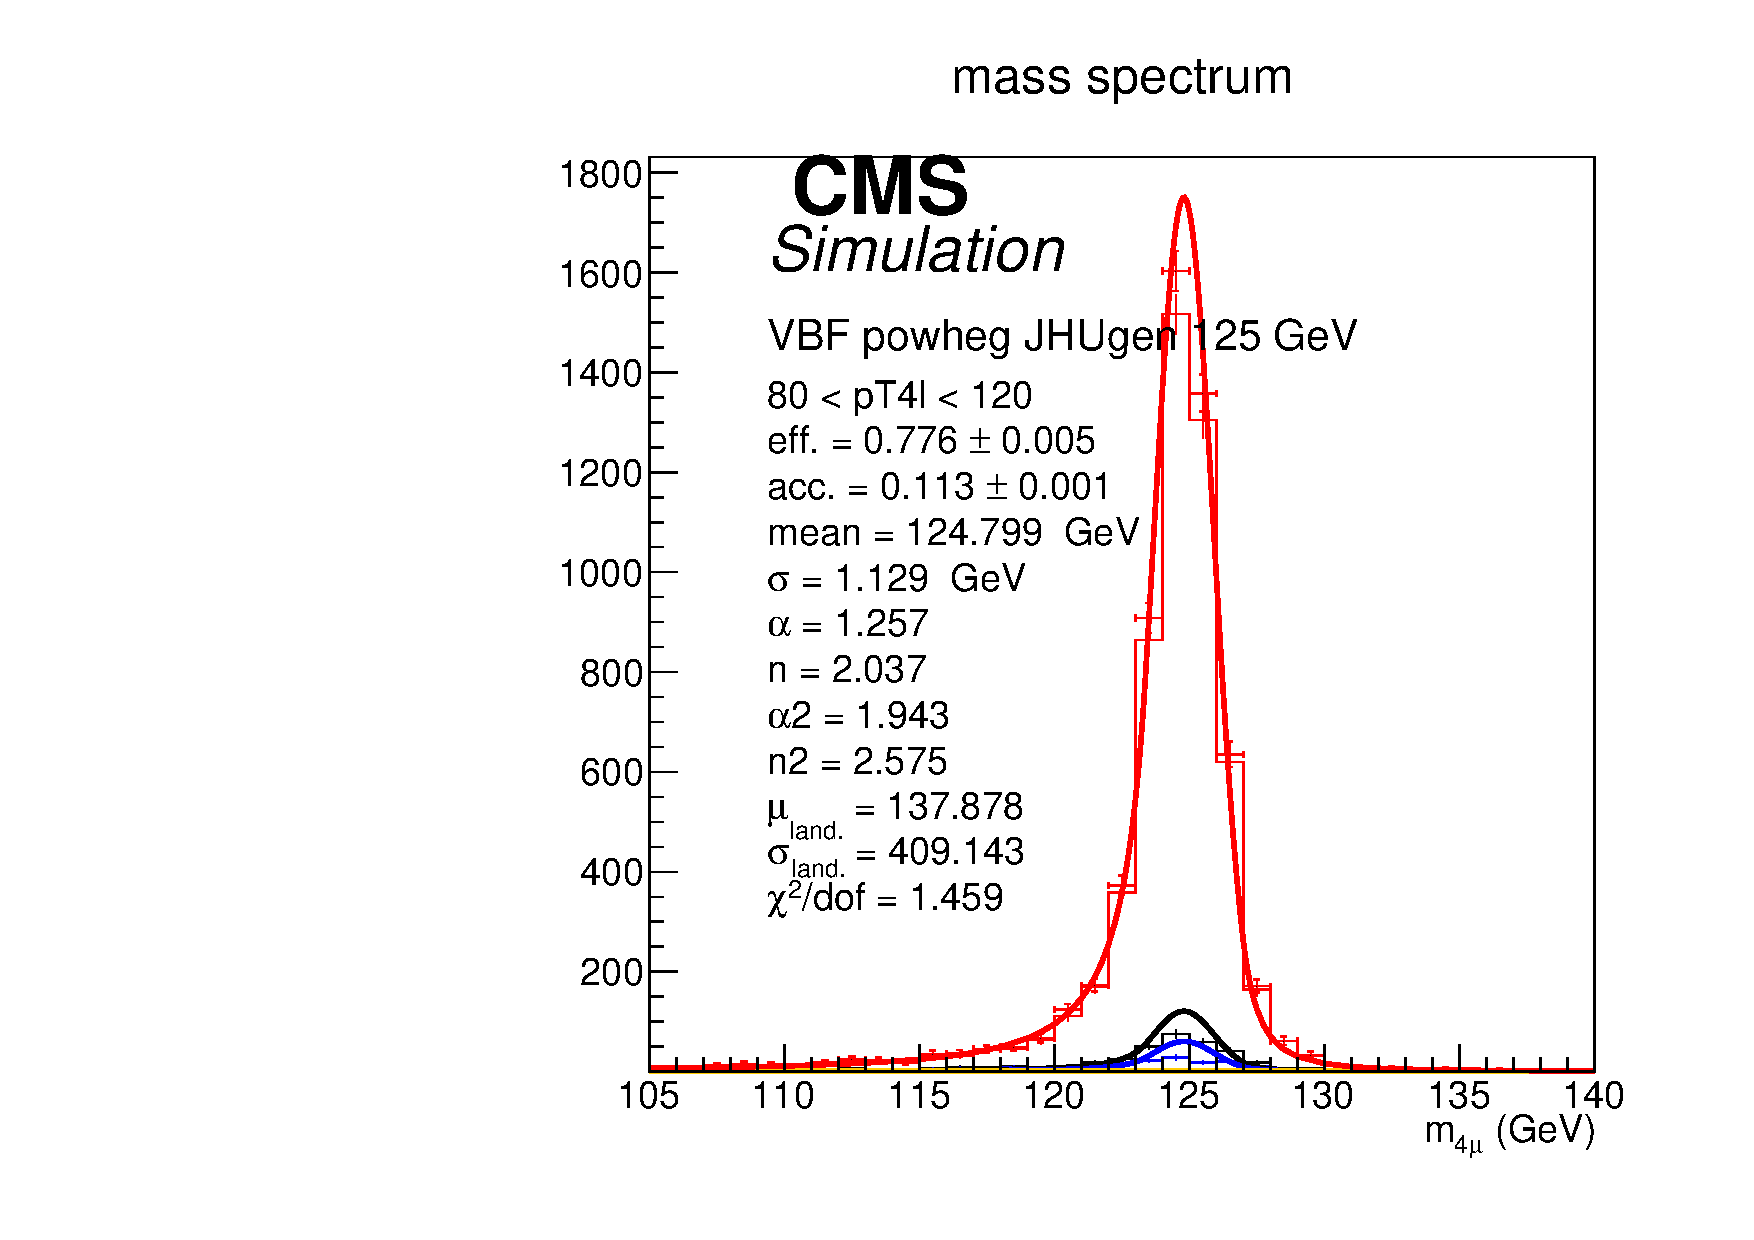
\includegraphics[width=0.3\textwidth,angle=0]{Figures/Appendix//VBF_powheg_JHUgen_125_4mu_pT4l_genbin4_recobin4_effs_genWeight*pileupWeight*dataMCWeight.pdf}
      \label{fig:sigfits-pT4l-VBF-powheg15-JHUgen-125-maintext:e}
    }
    \subfigure[$120.0 < \pt(\mathrm{H}) < 200.0$]{
      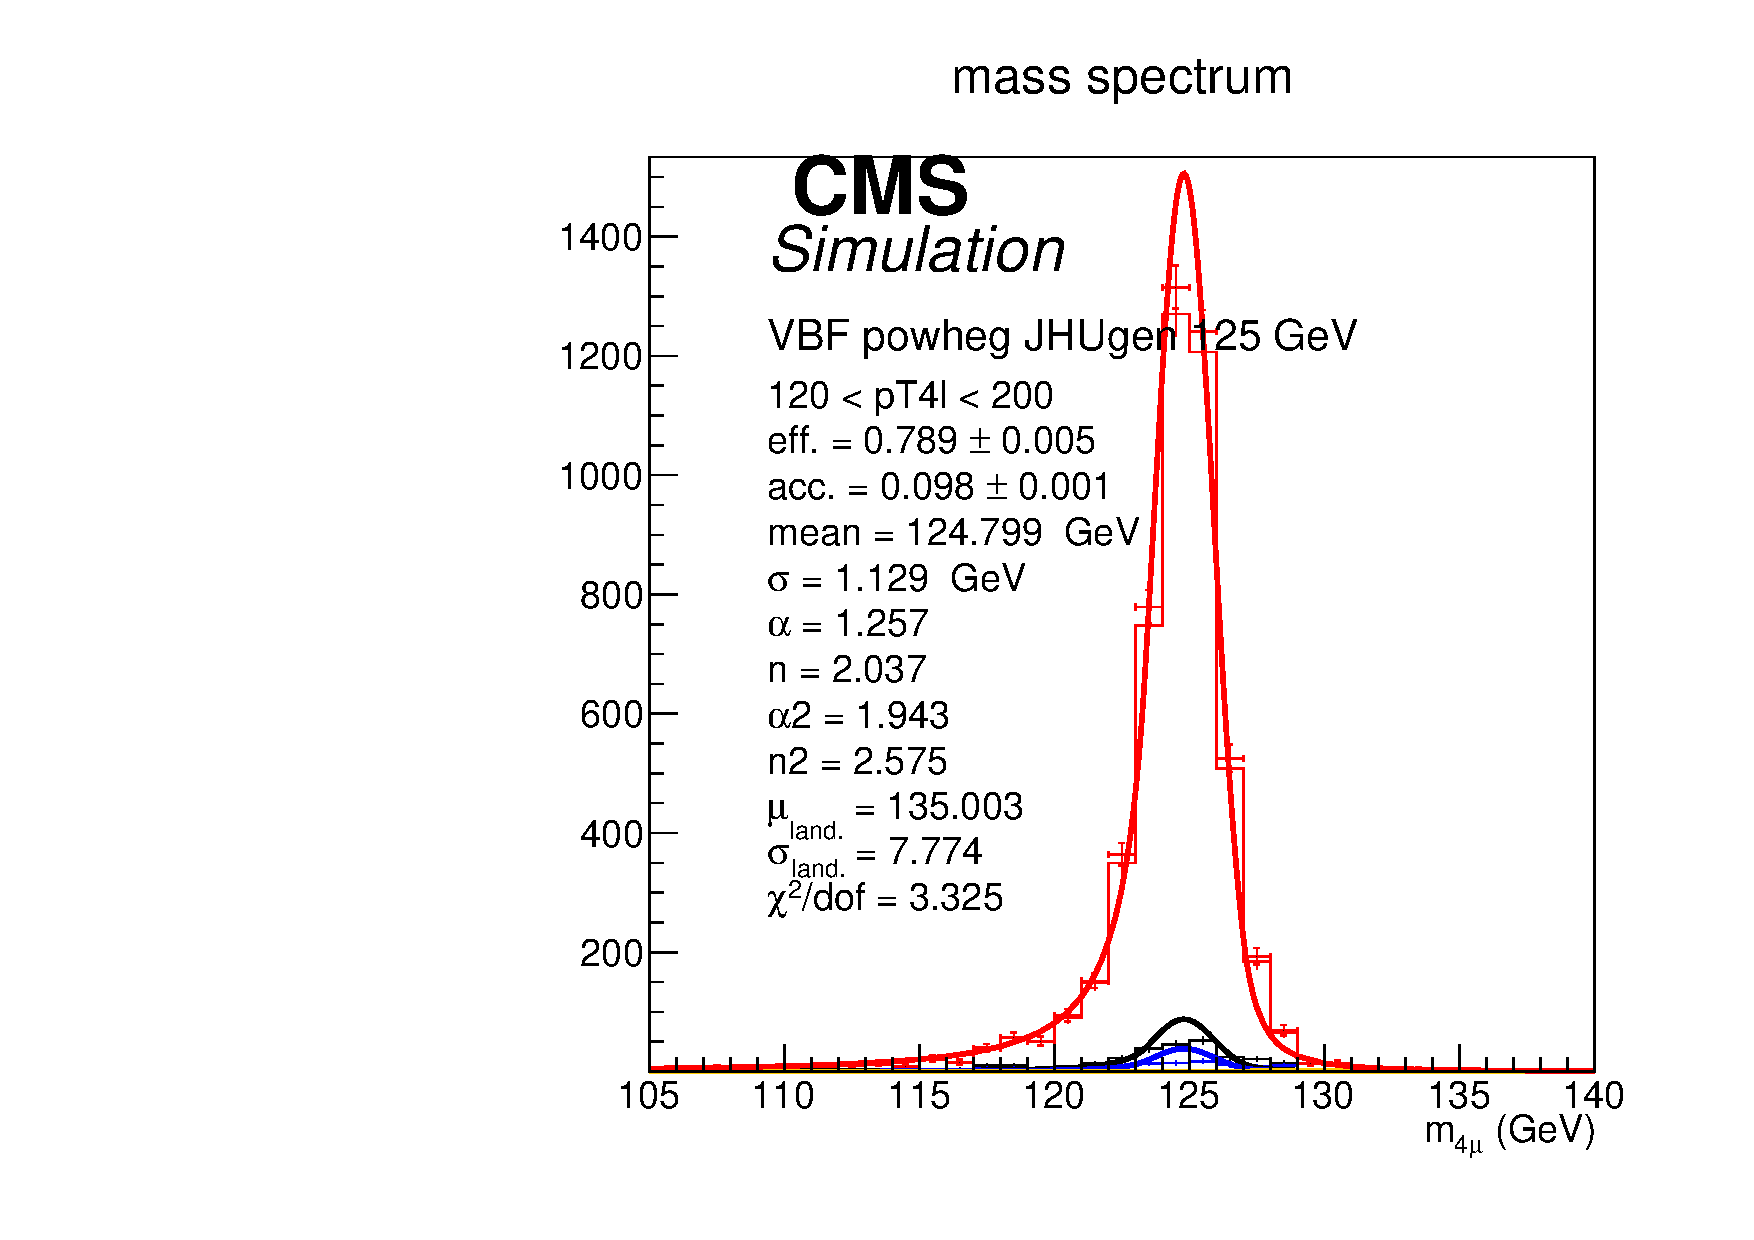
\includegraphics[width=0.3\textwidth,angle=0]{Figures/Appendix//VBF_powheg_JHUgen_125_4mu_pT4l_genbin5_recobin5_effs_genWeight*pileupWeight*dataMCWeight.pdf}
      \label{fig:sigfits-pT4l-VBF-powheg15-JHUgen-125-maintext:f}
    } \\
    \subfigure[$200.0 < \pt(\mathrm{H}) < 13000.0$]{
      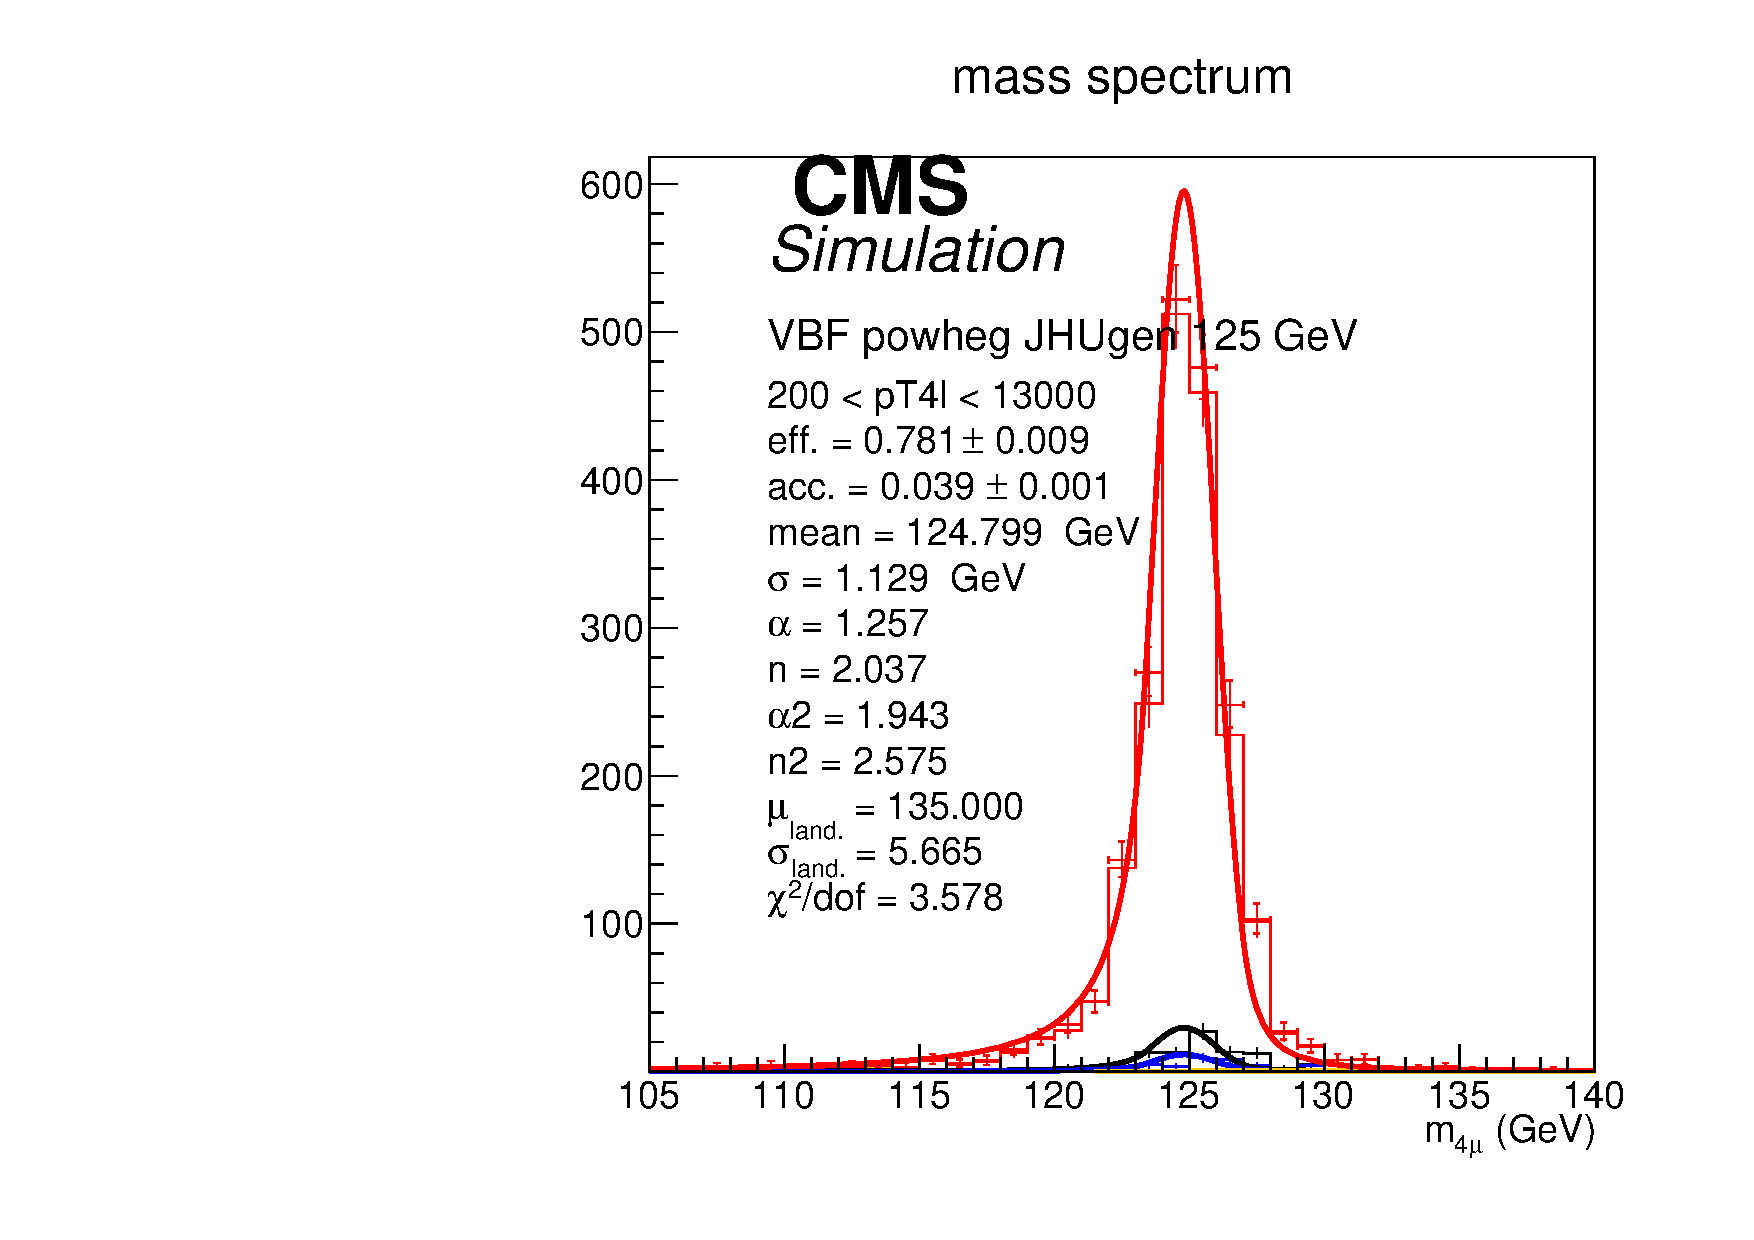
\includegraphics[width=0.3\textwidth,angle=0]{Figures/Appendix//VBF_powheg_JHUgen_125_4mu_pT4l_genbin6_recobin6_effs_genWeight*pileupWeight*dataMCWeight.pdf}
      \label{fig:sigfits-pT4l-VBF-powheg15-JHUgen-125-maintext:g}
    }
    \\
    \caption{ Example signal shapes at reconstruction level for a resonance of m(4$\ell$) in $4\mu$ final state for the $VBF$ production mode from {\sc powheg+JHUGen} in different bins of $\pt(\mathrm{H})$. The black curve represents events which do not pass the fiducial volume selection. The curve has no effect on the result.
    }
  \label{fig:sigfits-pT4l-VBF-powheg15-JHUgen-125-maintext}
 \end{center}
\end{figure} \clearpage


\begin{figure}[htb]
  \begin{center}
    \subfigure[$0.0 < \pt(\mathrm{H}) < 15.0 $]{
      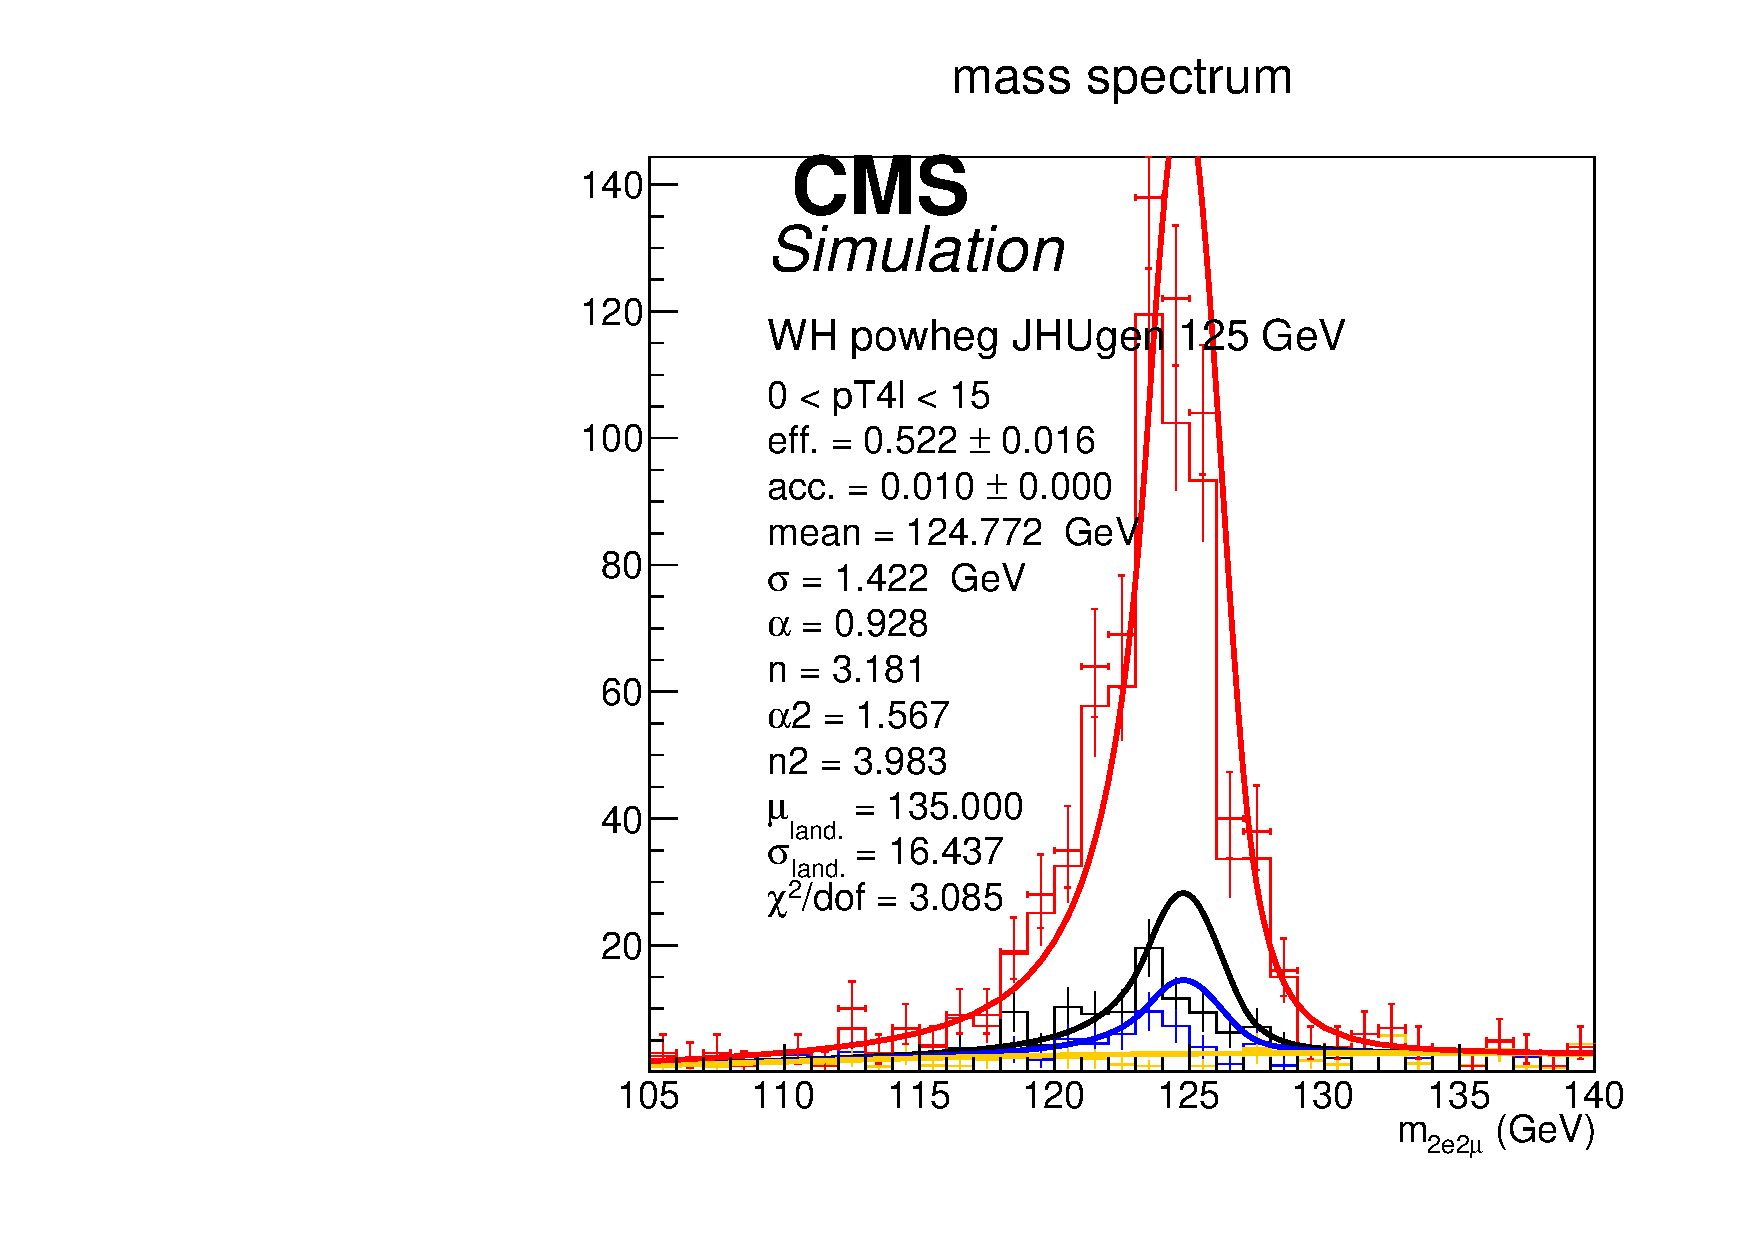
\includegraphics[width=0.3\textwidth,angle=0]{Figures/Appendix//WH_powheg_JHUgen_125_2e2mu_pT4l_genbin0_recobin0_effs_genWeight*pileupWeight*dataMCWeight.pdf}
      \label{fig:sigfits-pT4l-WH-powheg15-JHUgen-125-maintext:a}
    }
    \subfigure[$15.0 < \pt(\mathrm{H}) < 30.0$]{
      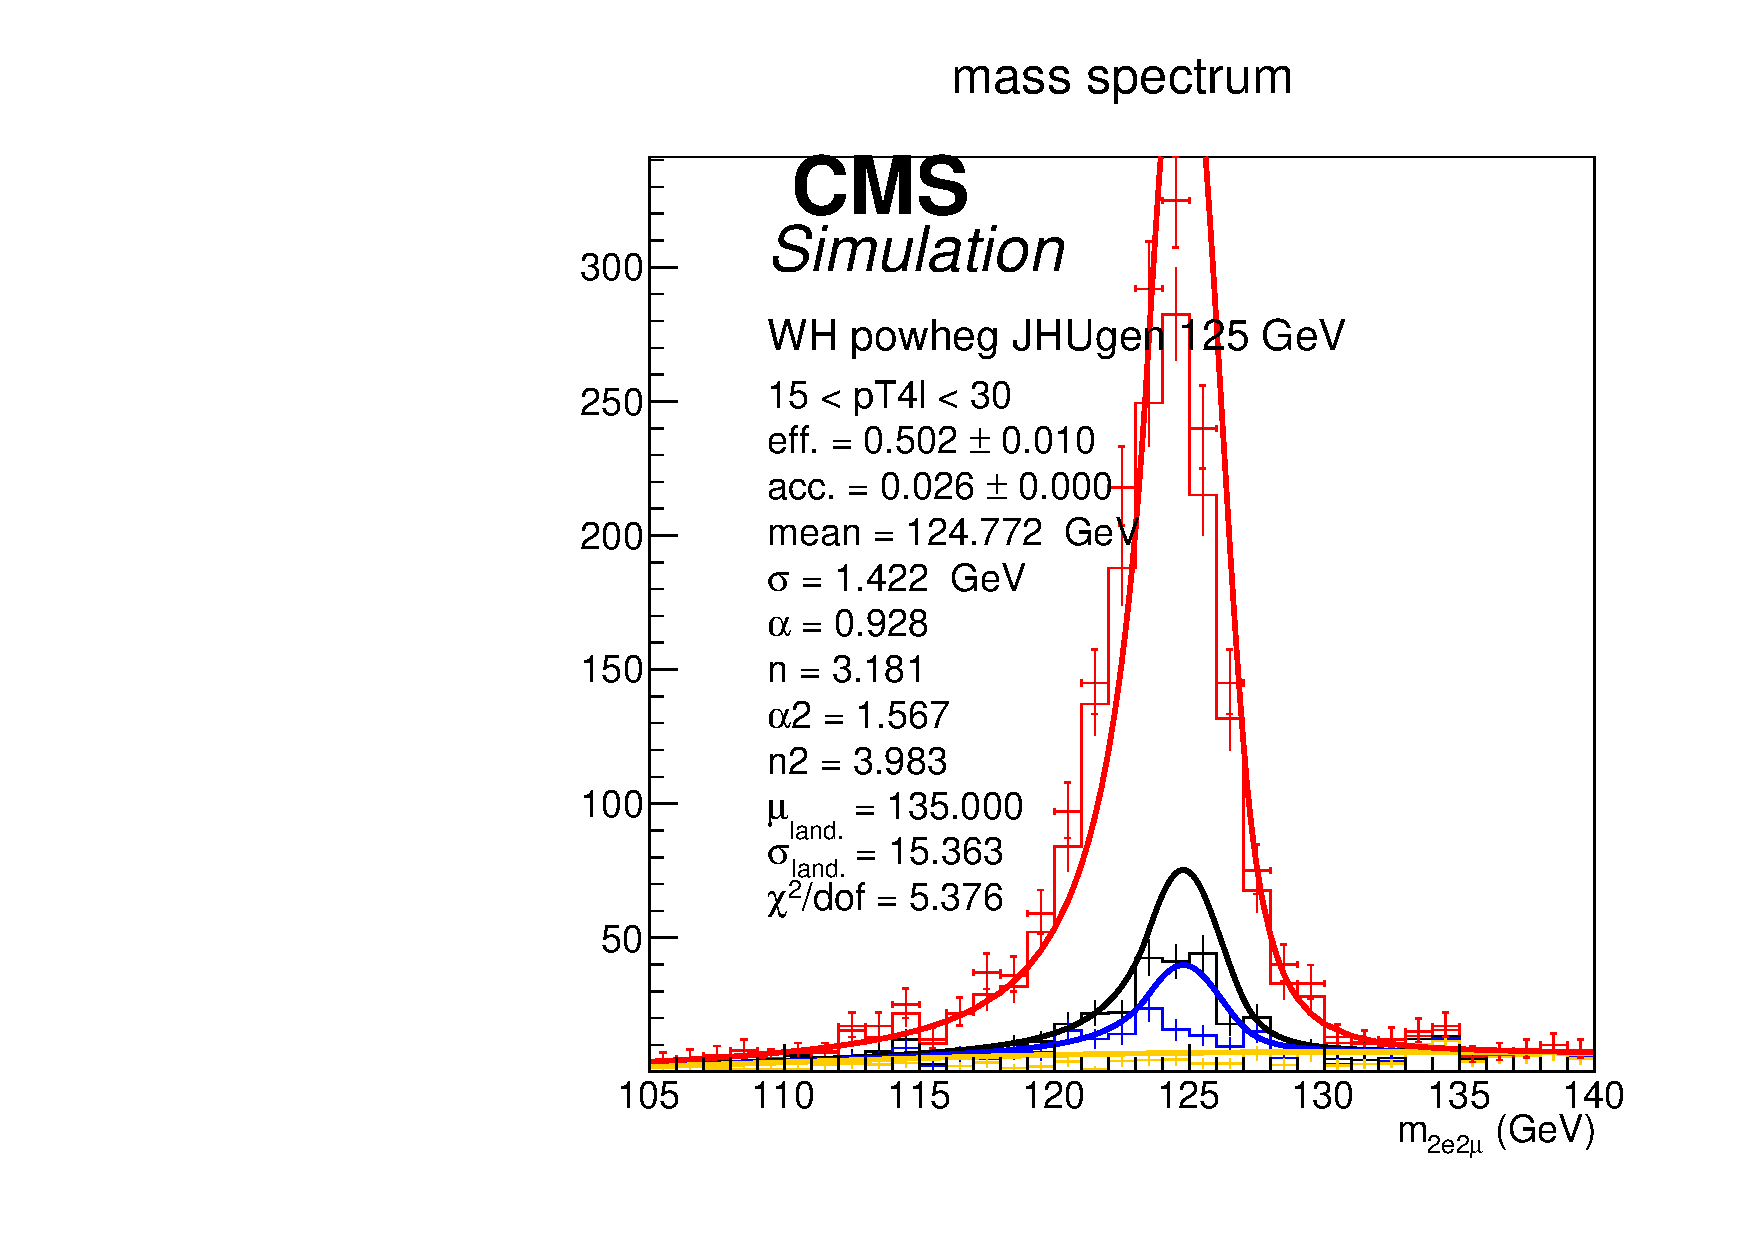
\includegraphics[width=0.3\textwidth,angle=0]{Figures/Appendix//WH_powheg_JHUgen_125_2e2mu_pT4l_genbin1_recobin1_effs_genWeight*pileupWeight*dataMCWeight.pdf}
      \label{fig:sigfits-pT4l-WH-powheg15-JHUgen-125-maintext:b}
    }
   \subfigure[$30.0 < \pt(\mathrm{H}) < 45.0$]{
      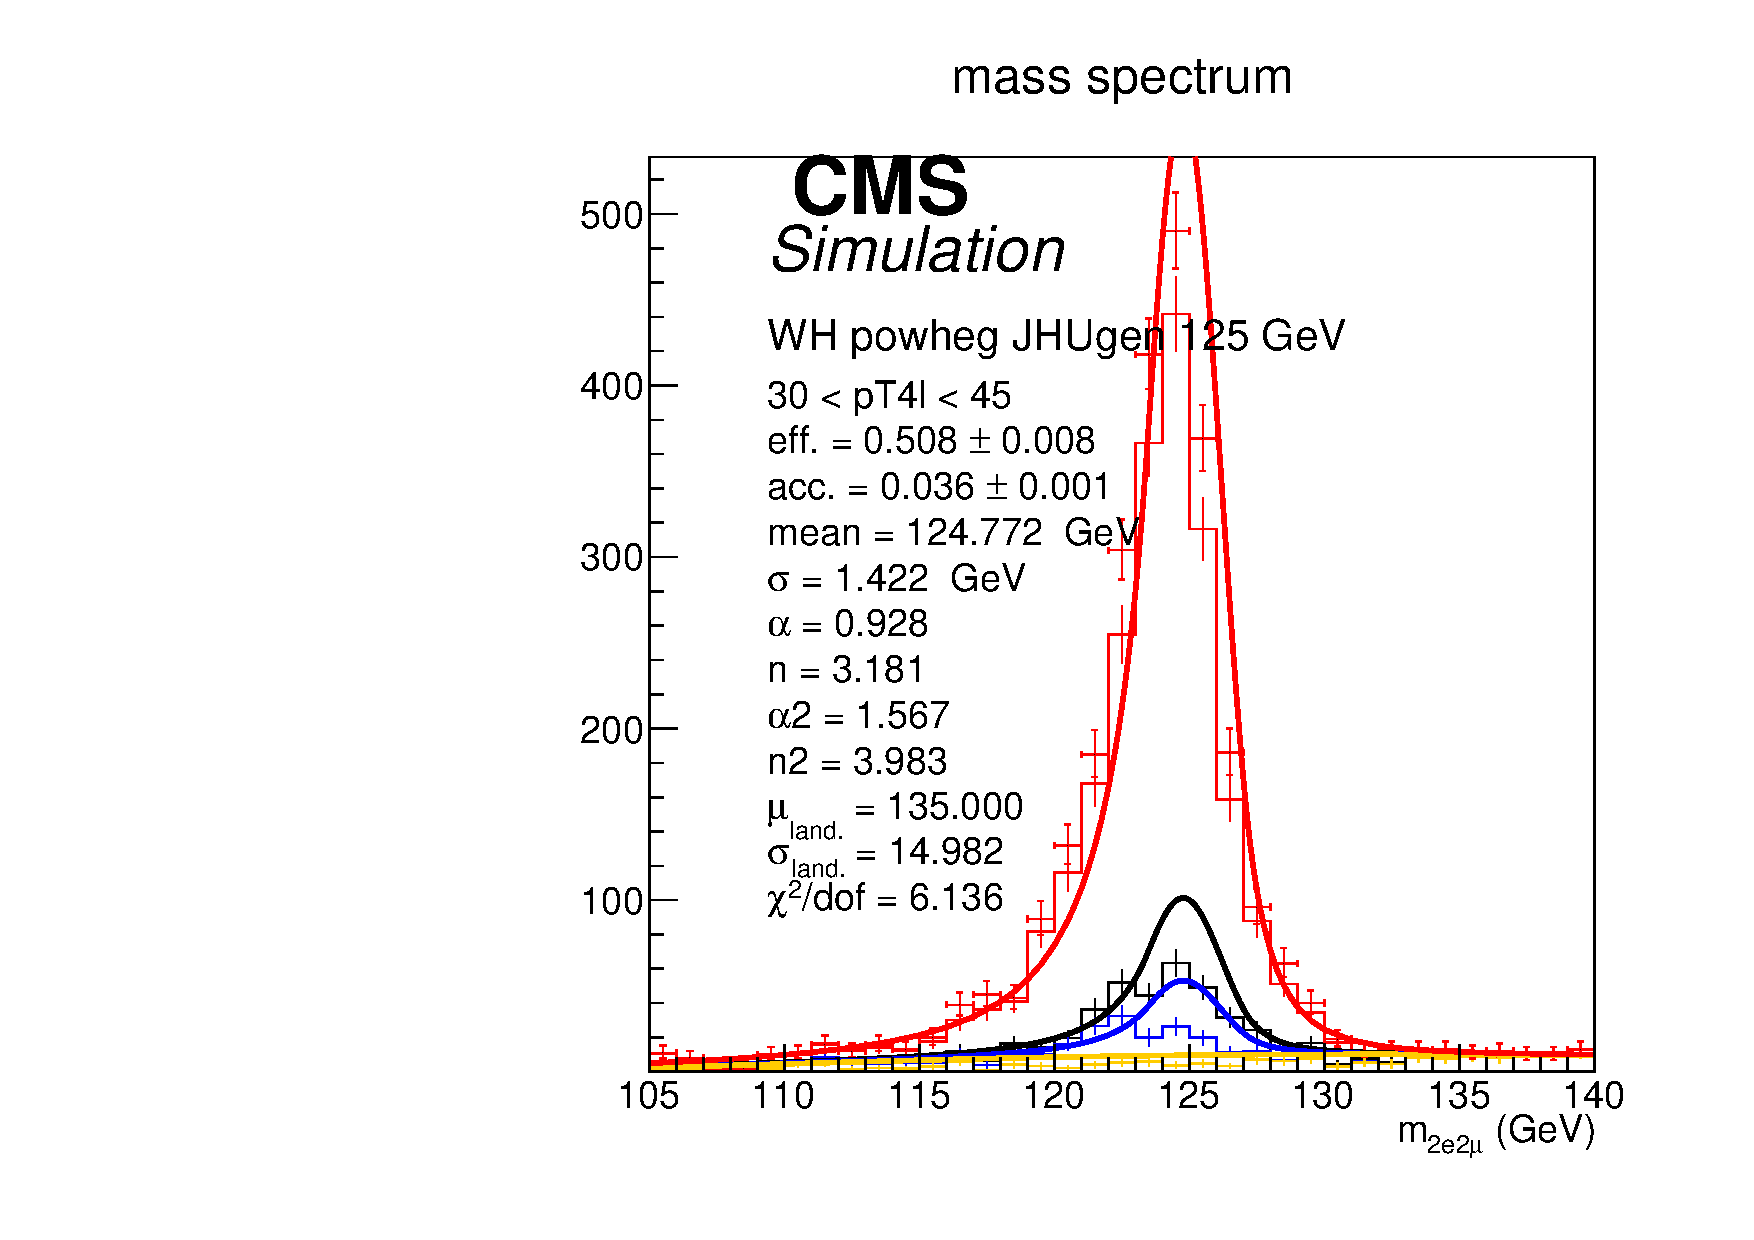
\includegraphics[width=0.3\textwidth,angle=0]{Figures/Appendix//WH_powheg_JHUgen_125_2e2mu_pT4l_genbin2_recobin2_effs_genWeight*pileupWeight*dataMCWeight.pdf}
      \label{fig:sigfits-pT4l-WH-powheg15-JHUgen-125-maintext:c}
    }  \\
    \subfigure[$45.0 < \pt(\mathrm{H}) < 80.0$]{
      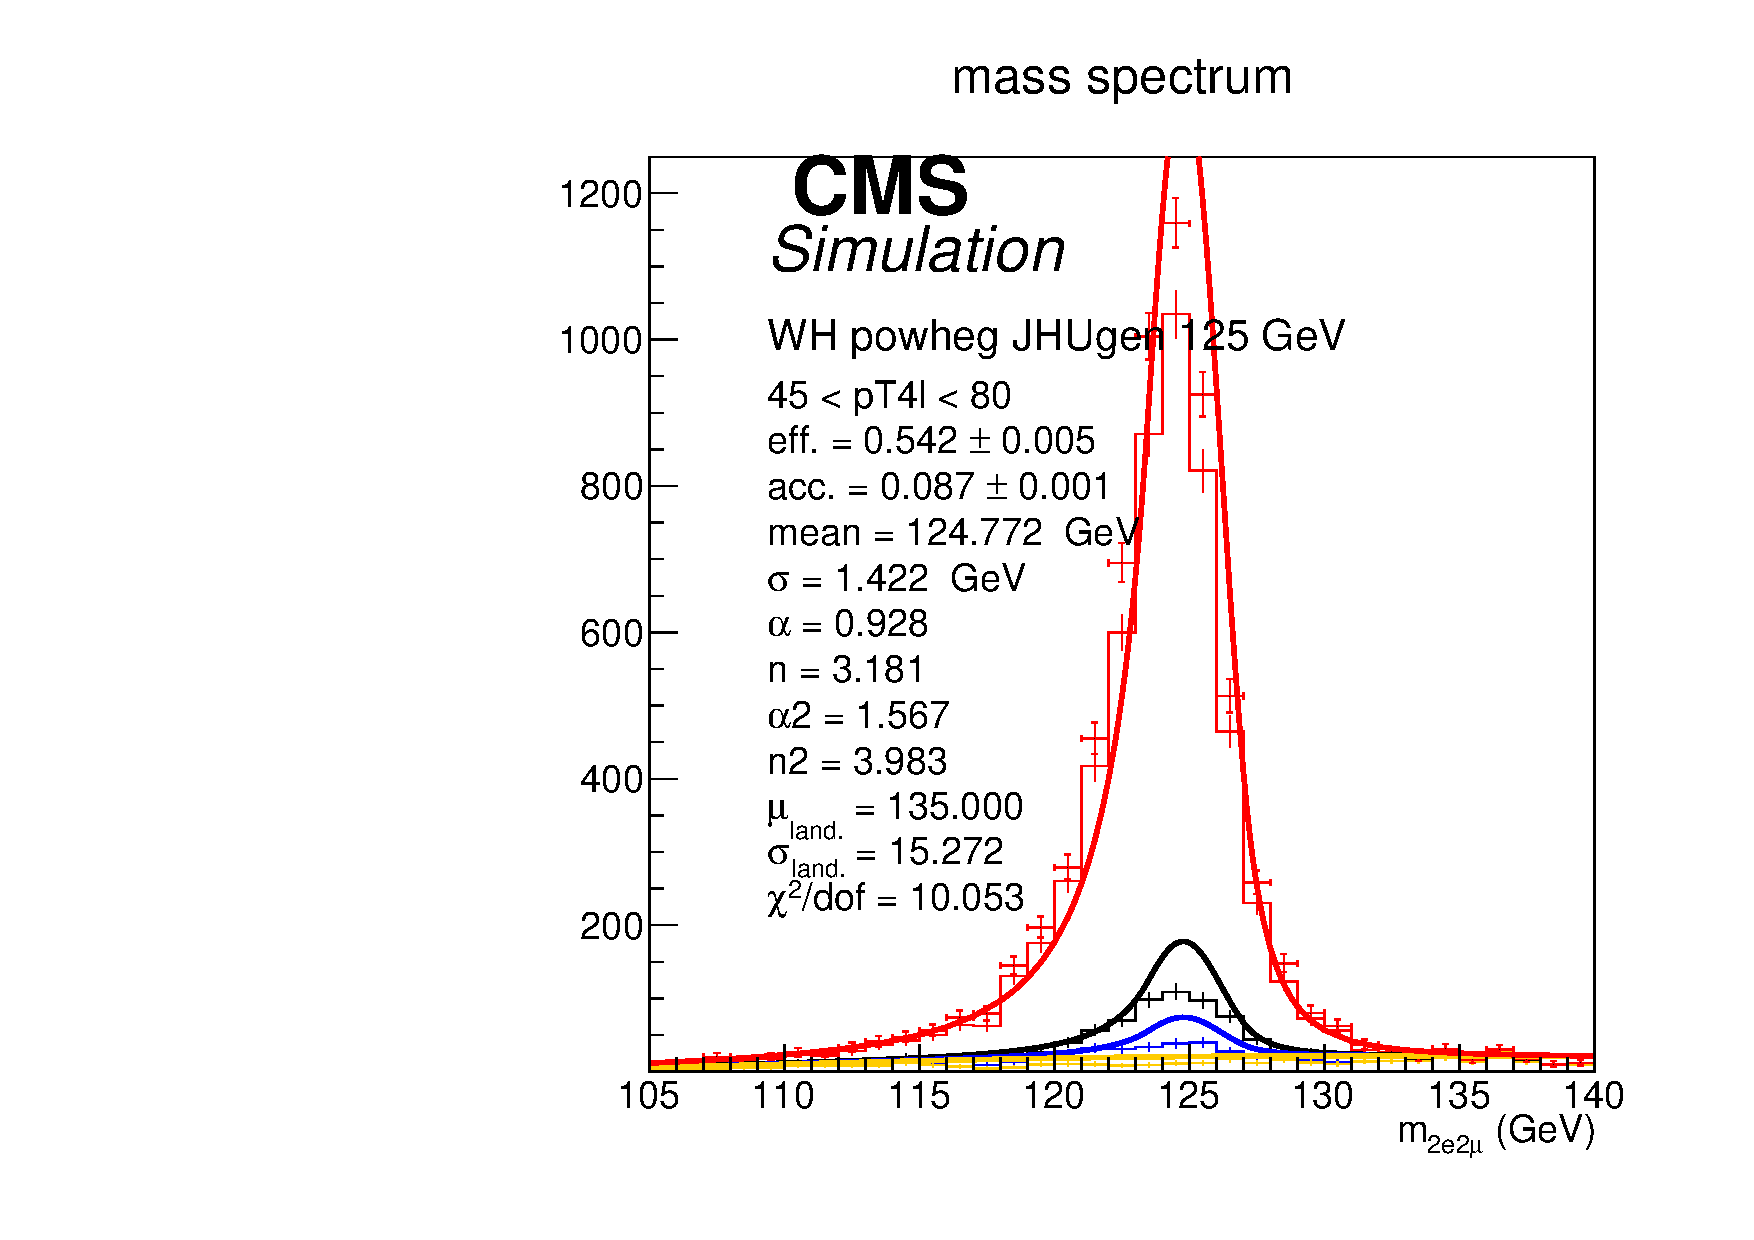
\includegraphics[width=0.3\textwidth,angle=0]{Figures/Appendix//WH_powheg_JHUgen_125_2e2mu_pT4l_genbin3_recobin3_effs_genWeight*pileupWeight*dataMCWeight.pdf}
      \label{fig:sigfits-pT4l-WH-powheg15-JHUgen-125-maintext:d}
    }
    \subfigure[$80.0 < \pt(\mathrm{H}) < 120.0$]{
      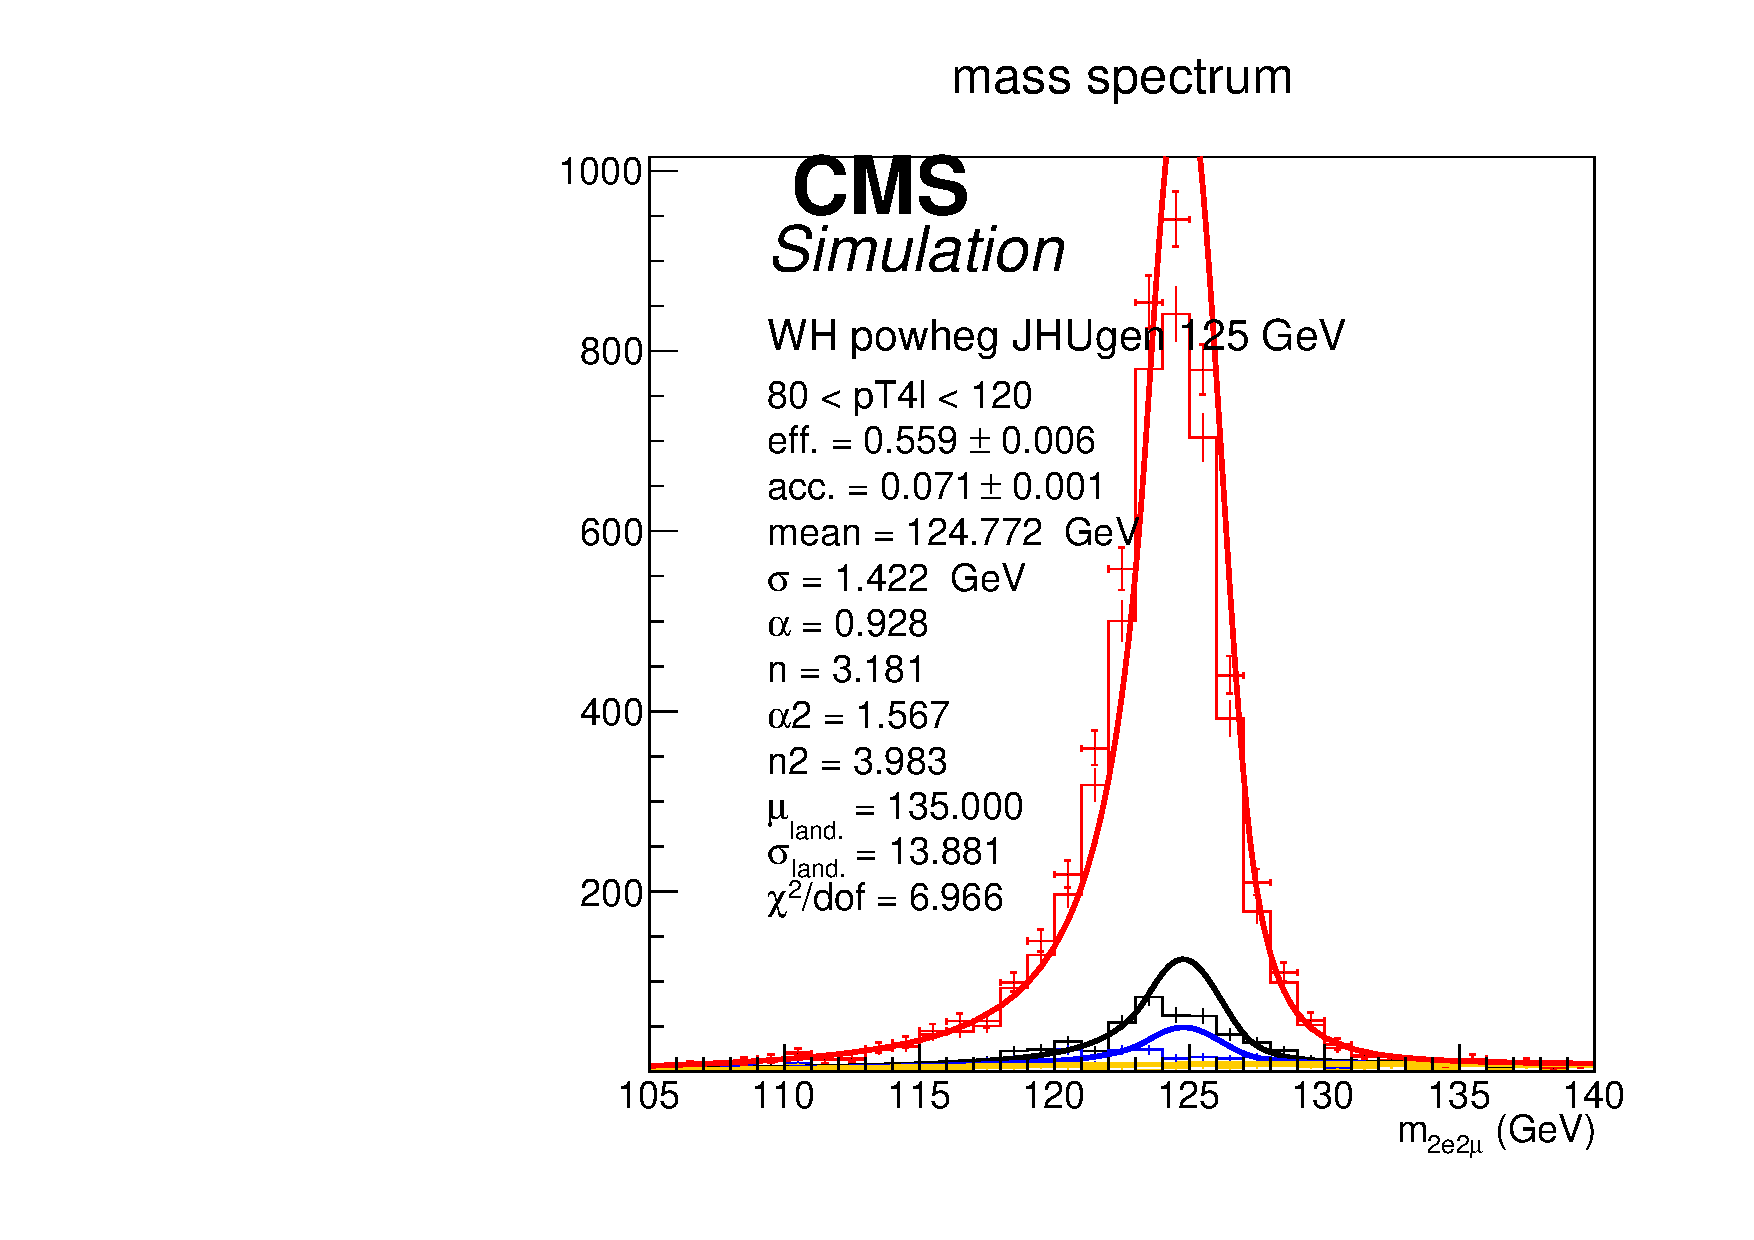
\includegraphics[width=0.3\textwidth,angle=0]{Figures/Appendix//WH_powheg_JHUgen_125_2e2mu_pT4l_genbin4_recobin4_effs_genWeight*pileupWeight*dataMCWeight.pdf}
      \label{fig:sigfits-pT4l-WH-powheg15-JHUgen-125-maintext:e}
    }
    \subfigure[$120.0 < \pt(\mathrm{H}) < 200.0$]{
      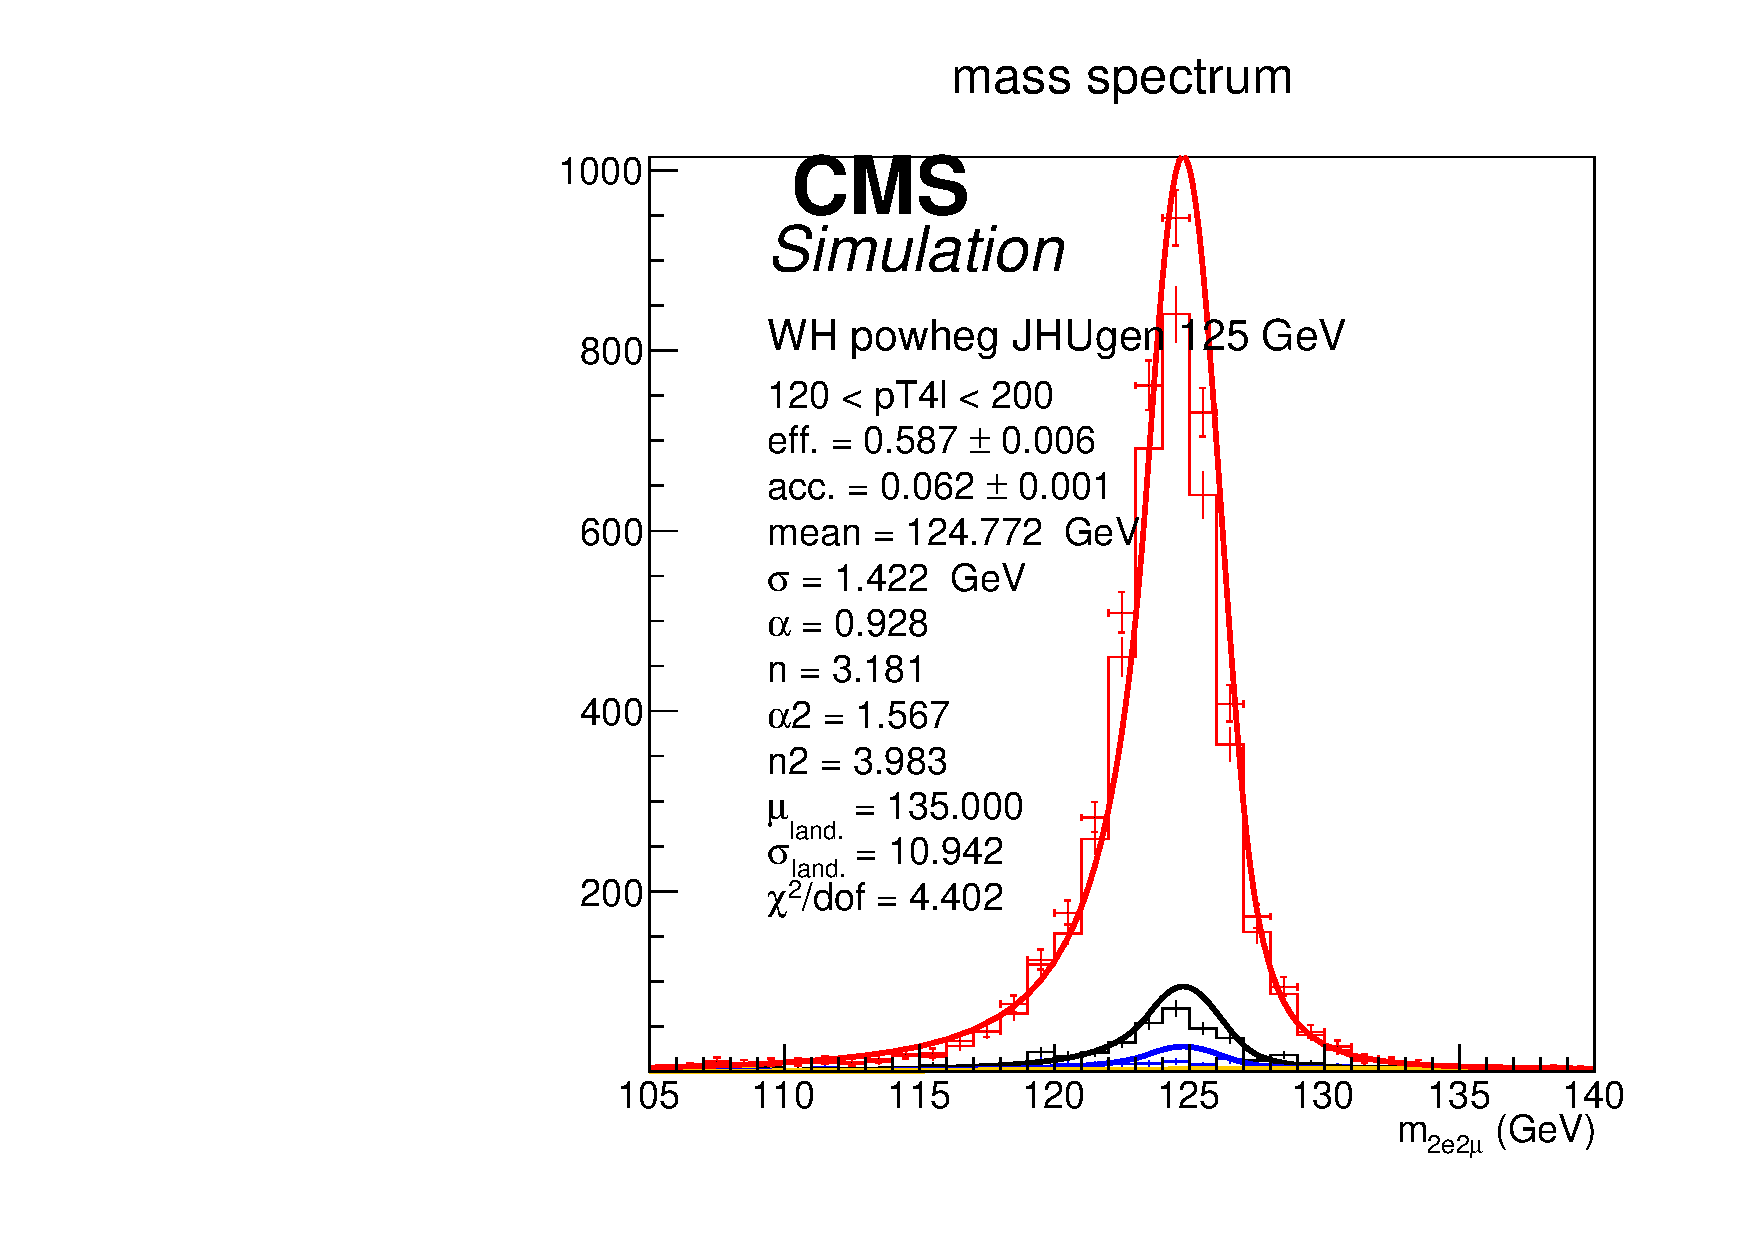
\includegraphics[width=0.3\textwidth,angle=0]{Figures/Appendix//WH_powheg_JHUgen_125_2e2mu_pT4l_genbin5_recobin5_effs_genWeight*pileupWeight*dataMCWeight.pdf}
      \label{fig:sigfits-pT4l-WH-powheg15-JHUgen-125-maintext:f}
    } \\
    \subfigure[$200.0 < \pt(\mathrm{H}) < 13000.0$]{
      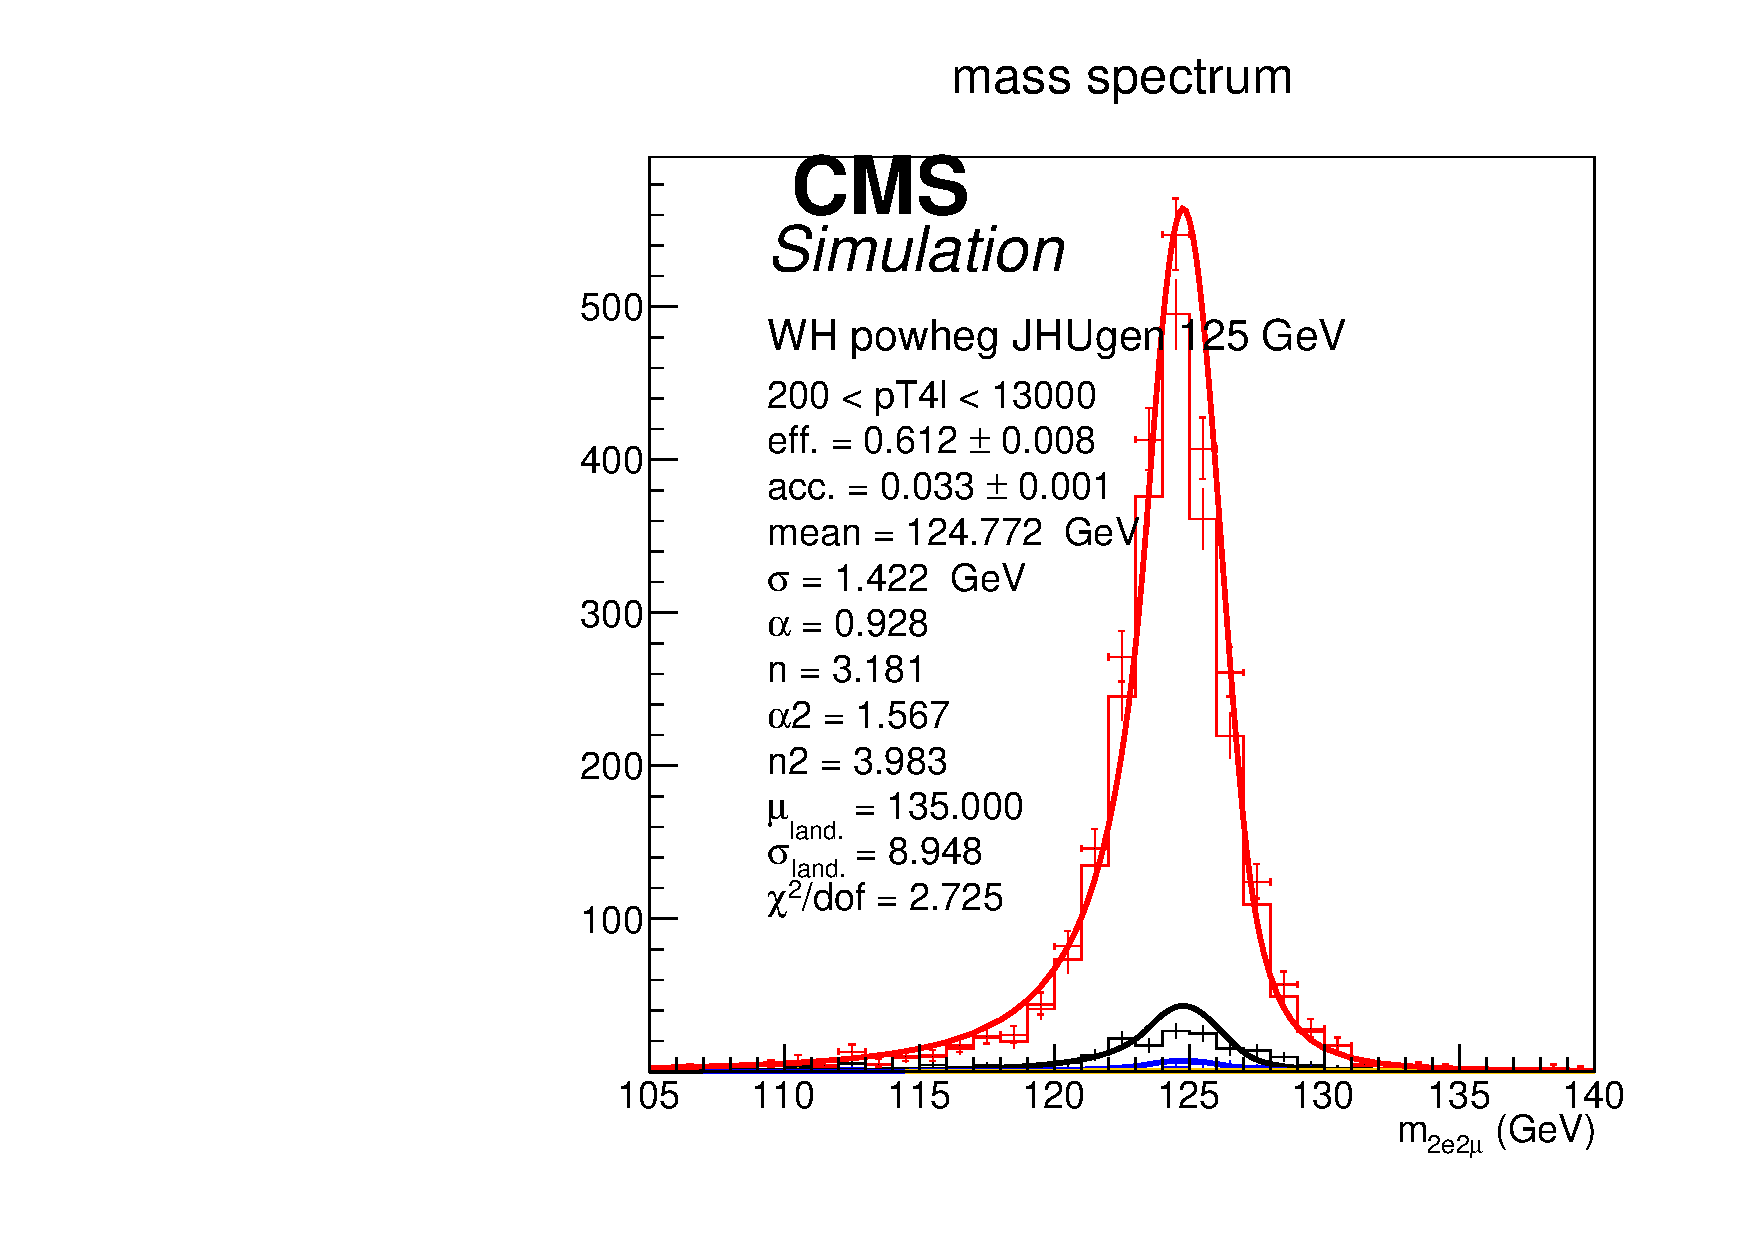
\includegraphics[width=0.3\textwidth,angle=0]{Figures/Appendix//WH_powheg_JHUgen_125_2e2mu_pT4l_genbin6_recobin6_effs_genWeight*pileupWeight*dataMCWeight.pdf}
      \label{fig:sigfits-pT4l-WH-powheg15-JHUgen-125-maintext:g}
    }
    \\
    \caption{ Example signal shapes at reconstruction level for a resonance of m(4$\ell$) in $2e2\mu$ final state for the $WH$ production mode from {\sc powheg+JHUGen} in different bins of $\pt(\mathrm{H})$. The black curve represents events which do not pass the fiducial volume selection. The curve has no effect on the result.
    }
  \label{fig:sigfits-pT4l-WH-powheg15-JHUgen-125-maintext}
 \end{center}
\end{figure} \clearpage

\begin{figure}[htb]
  \begin{center}
    \subfigure[$0.0 < \pt(\mathrm{H}) < 15.0 $]{
      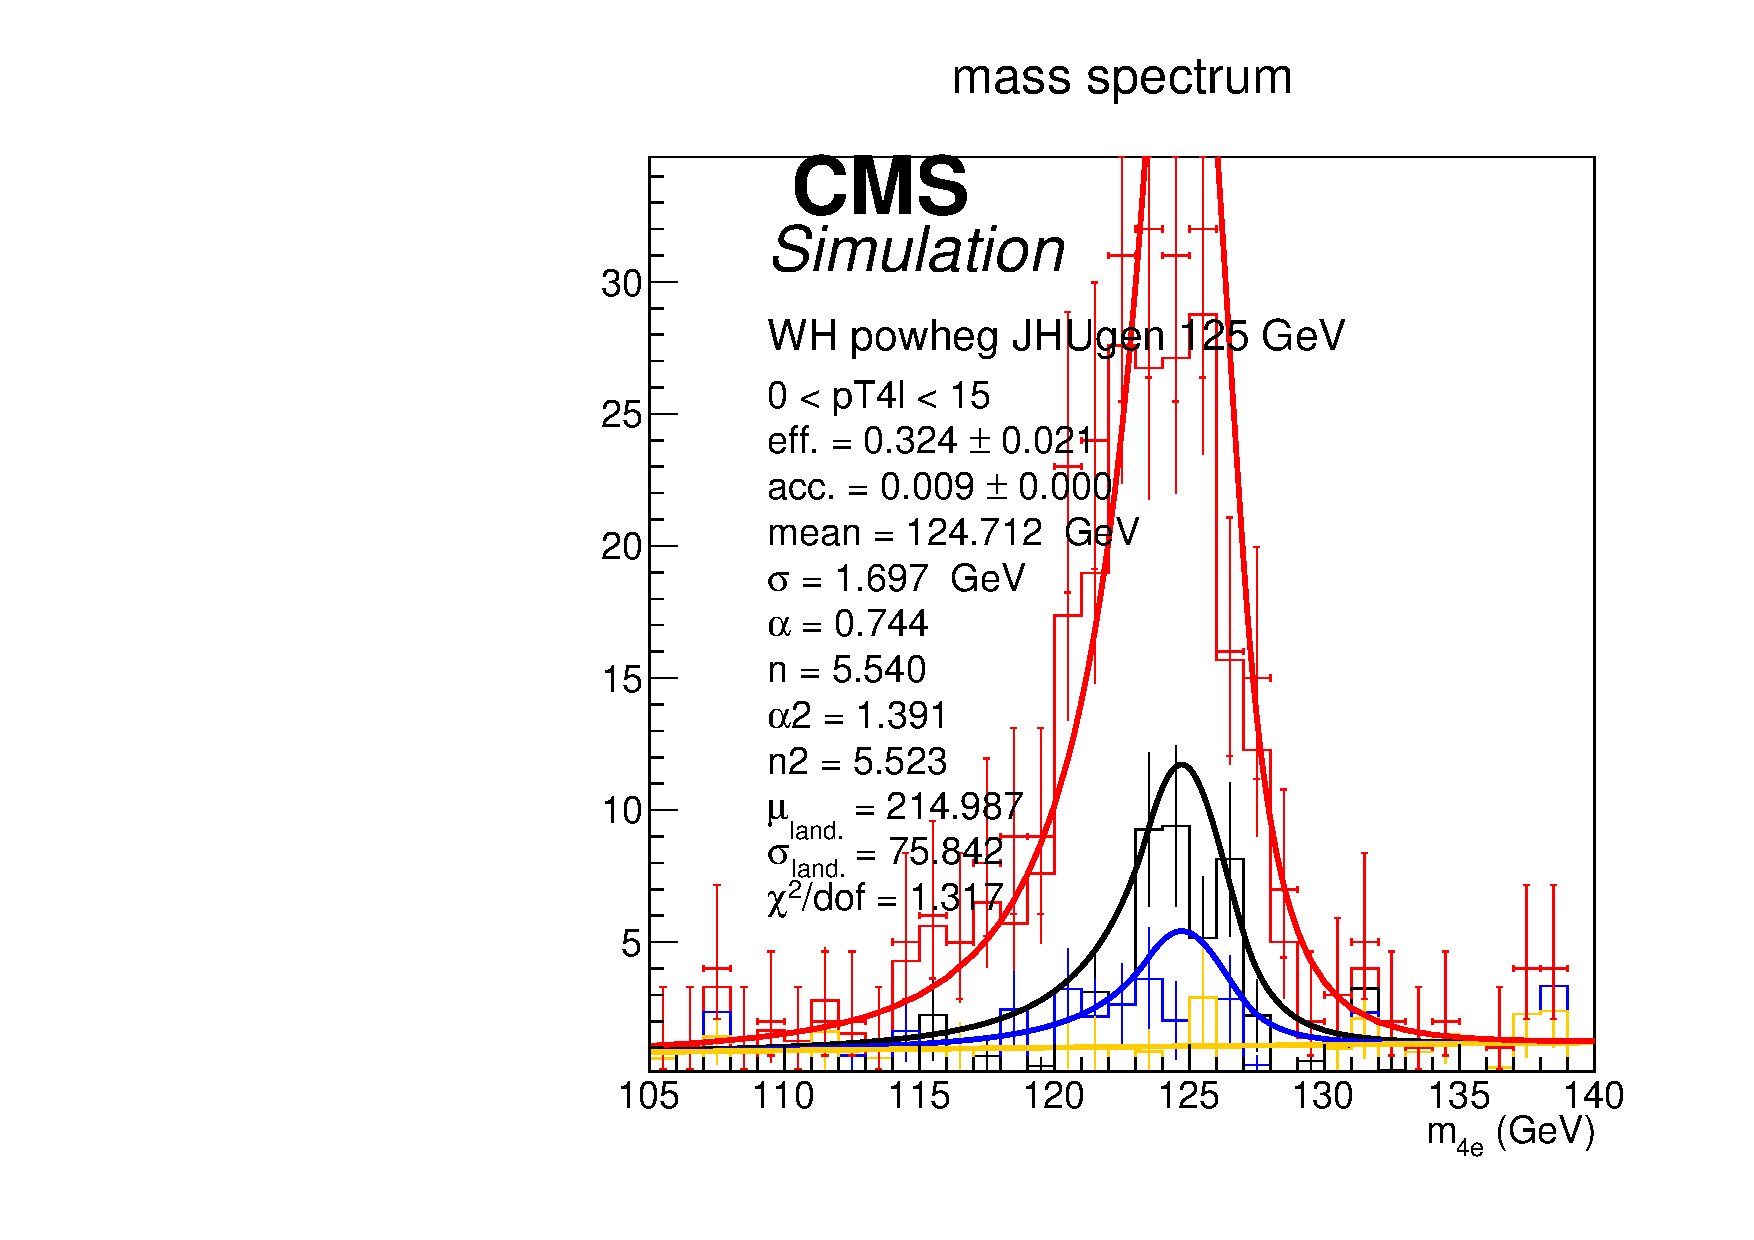
\includegraphics[width=0.3\textwidth,angle=0]{Figures/Appendix//WH_powheg_JHUgen_125_4e_pT4l_genbin0_recobin0_effs_genWeight*pileupWeight*dataMCWeight.pdf}
      \label{fig:sigfits-pT4l-WH-powheg15-JHUgen-125-maintext:a}
    }
    \subfigure[$15.0 < \pt(\mathrm{H}) < 30.0$]{
      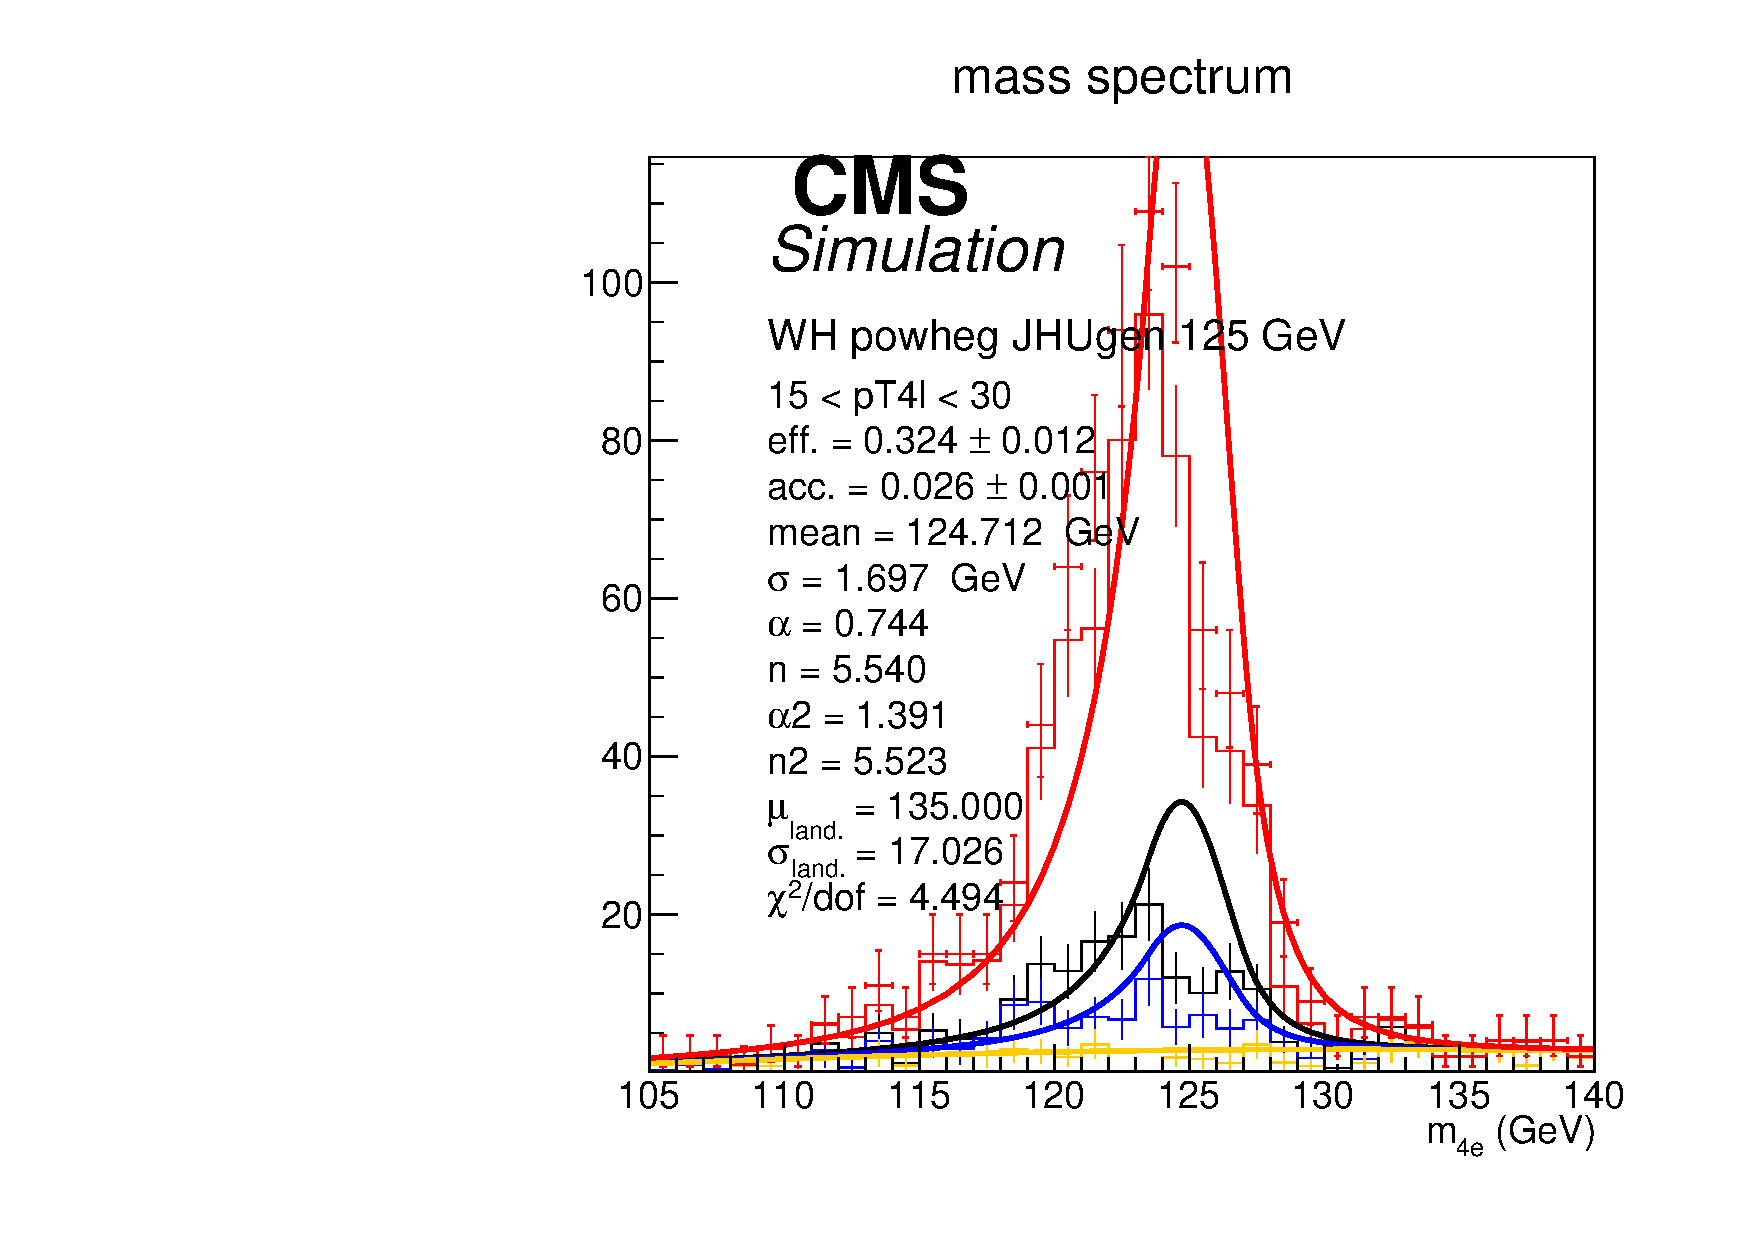
\includegraphics[width=0.3\textwidth,angle=0]{Figures/Appendix//WH_powheg_JHUgen_125_4e_pT4l_genbin1_recobin1_effs_genWeight*pileupWeight*dataMCWeight.pdf}
      \label{fig:sigfits-pT4l-WH-powheg15-JHUgen-125-maintext:b}
    }
   \subfigure[$30.0 < \pt(\mathrm{H}) < 45.0$]{
      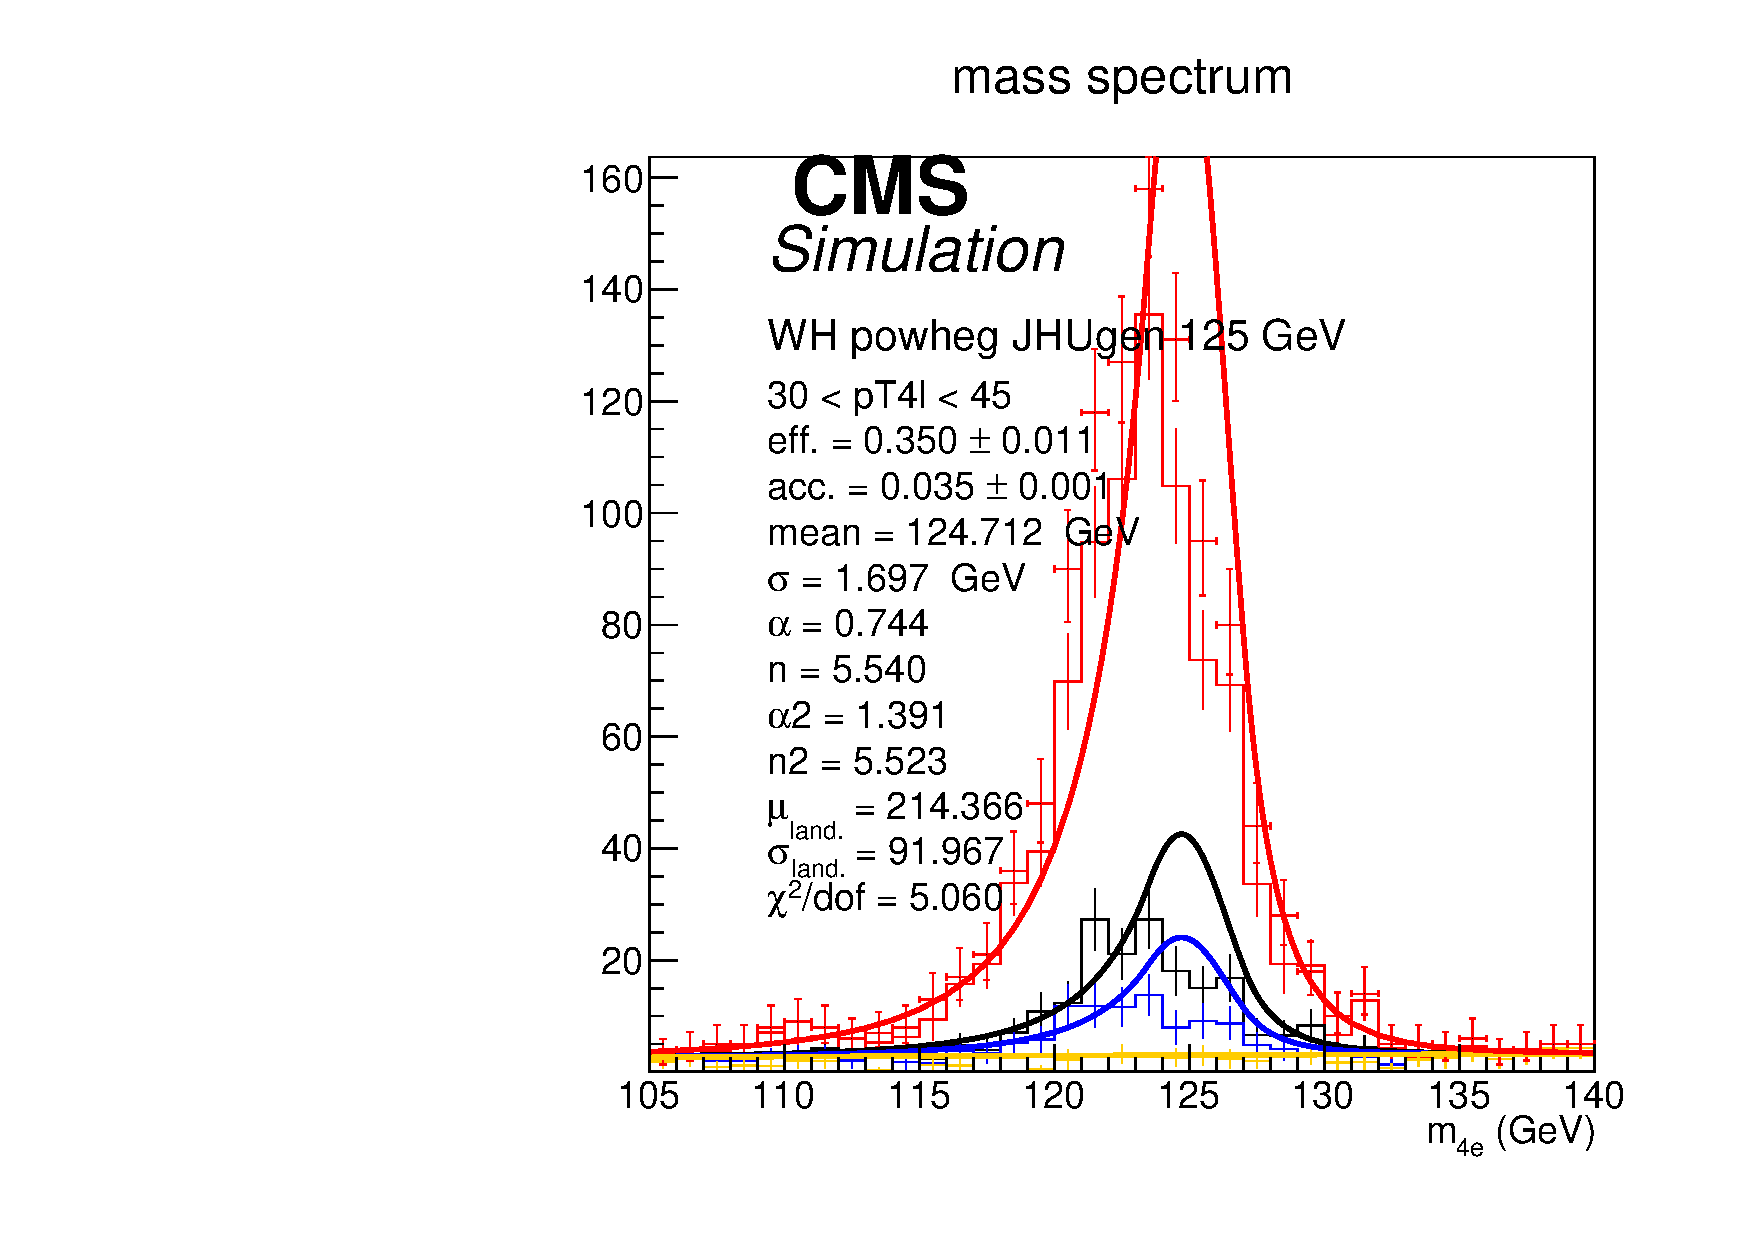
\includegraphics[width=0.3\textwidth,angle=0]{Figures/Appendix//WH_powheg_JHUgen_125_4e_pT4l_genbin2_recobin2_effs_genWeight*pileupWeight*dataMCWeight.pdf}
      \label{fig:sigfits-pT4l-WH-powheg15-JHUgen-125-maintext:c}
    }  \\
    \subfigure[$45.0 < \pt(\mathrm{H}) < 80.0$]{
      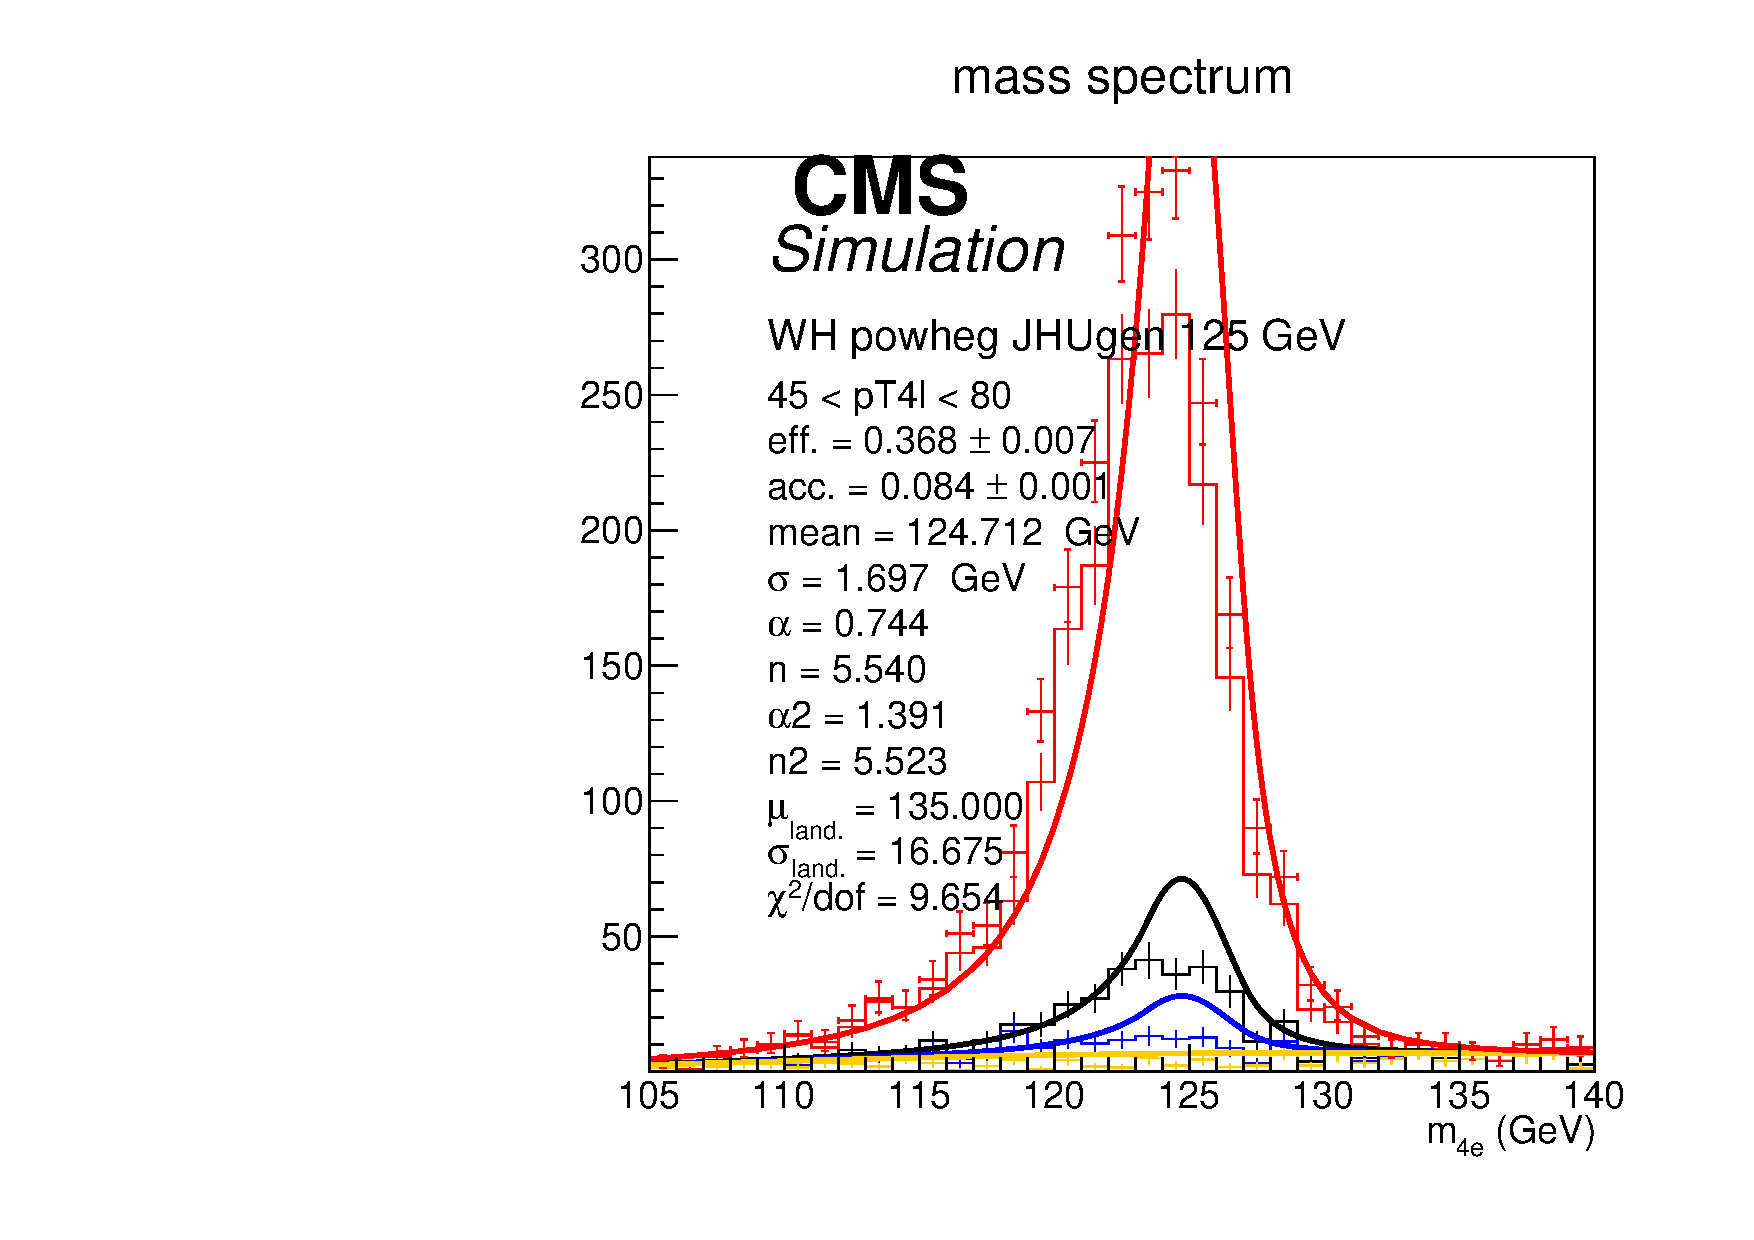
\includegraphics[width=0.3\textwidth,angle=0]{Figures/Appendix//WH_powheg_JHUgen_125_4e_pT4l_genbin3_recobin3_effs_genWeight*pileupWeight*dataMCWeight.pdf}
      \label{fig:sigfits-pT4l-WH-powheg15-JHUgen-125-maintext:d}
    }
    \subfigure[$80.0 < \pt(\mathrm{H}) < 120.0$]{
      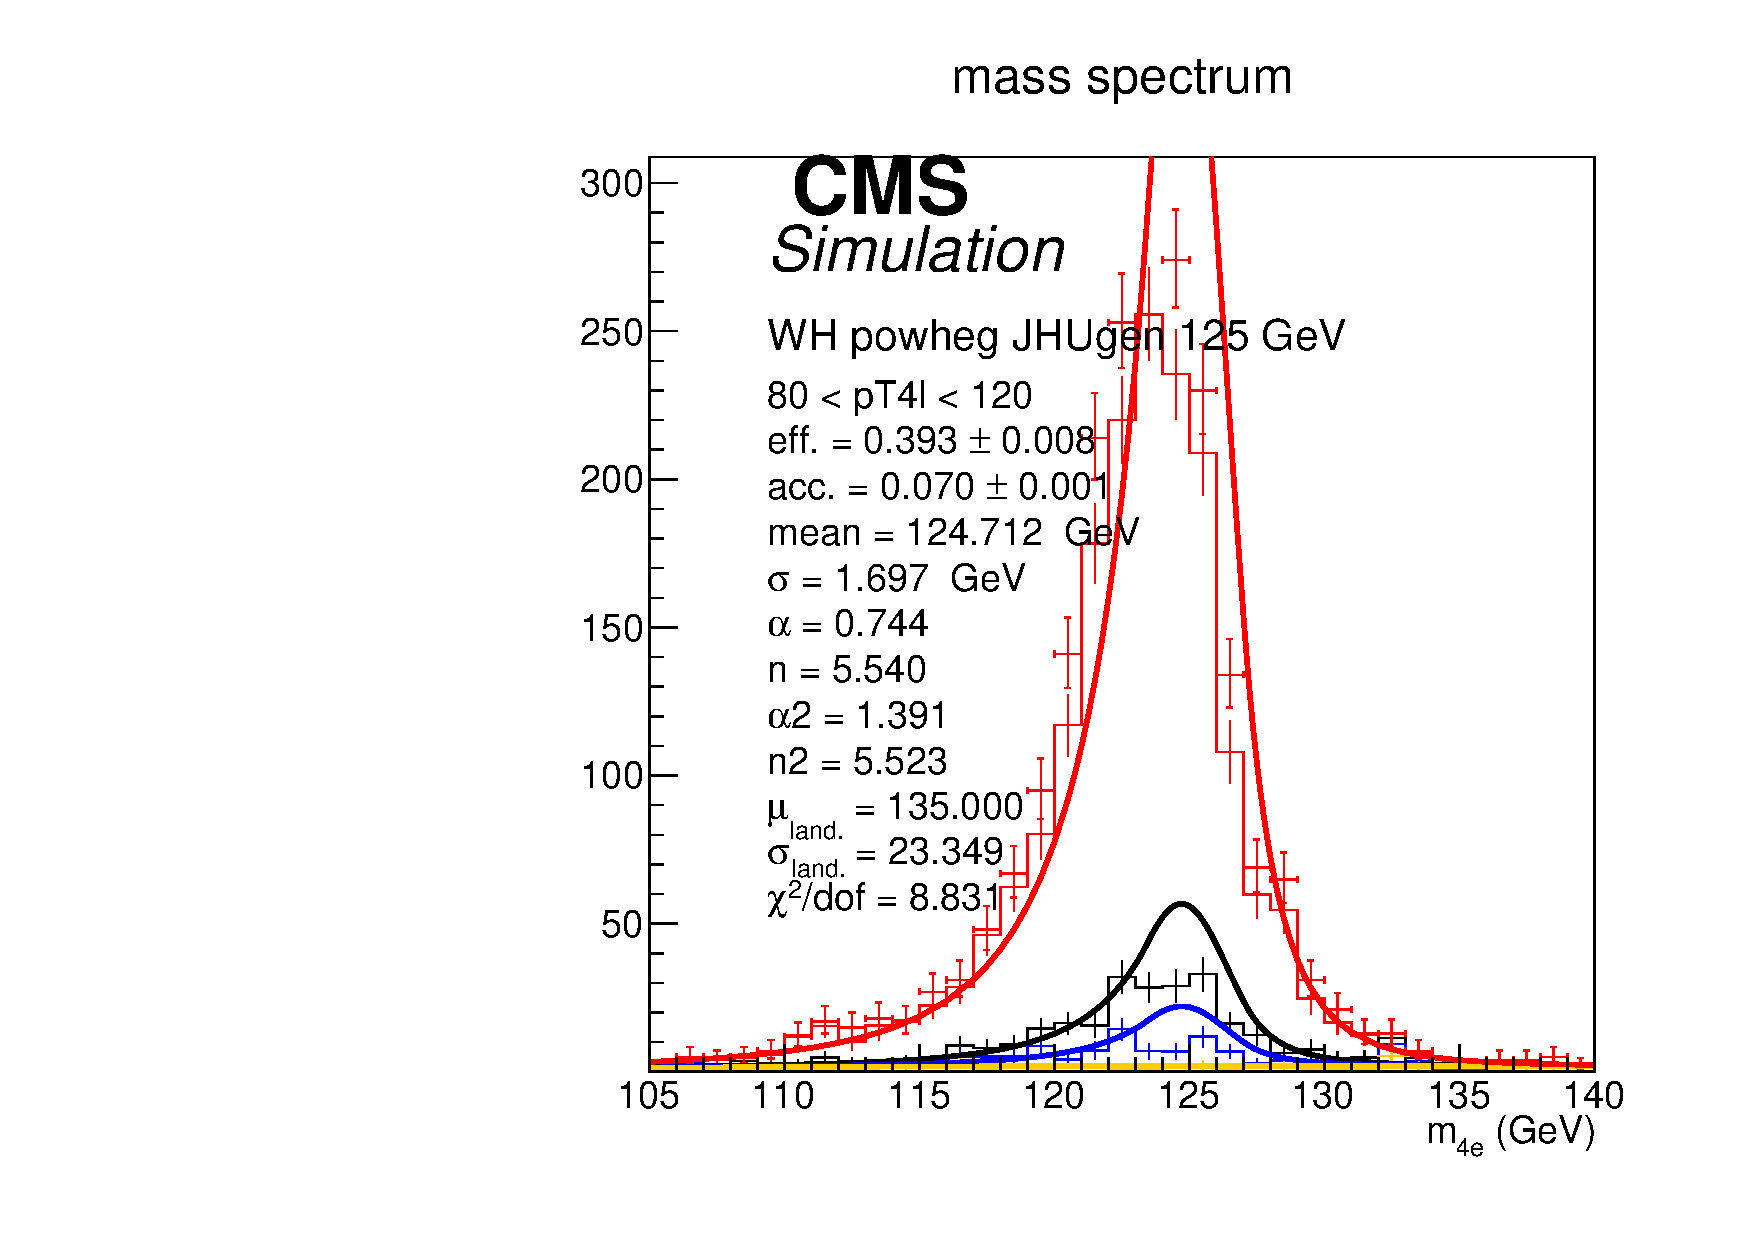
\includegraphics[width=0.3\textwidth,angle=0]{Figures/Appendix//WH_powheg_JHUgen_125_4e_pT4l_genbin4_recobin4_effs_genWeight*pileupWeight*dataMCWeight.pdf}
      \label{fig:sigfits-pT4l-WH-powheg15-JHUgen-125-maintext:e}
    }
    \subfigure[$120.0 < \pt(\mathrm{H}) < 200.0$]{
      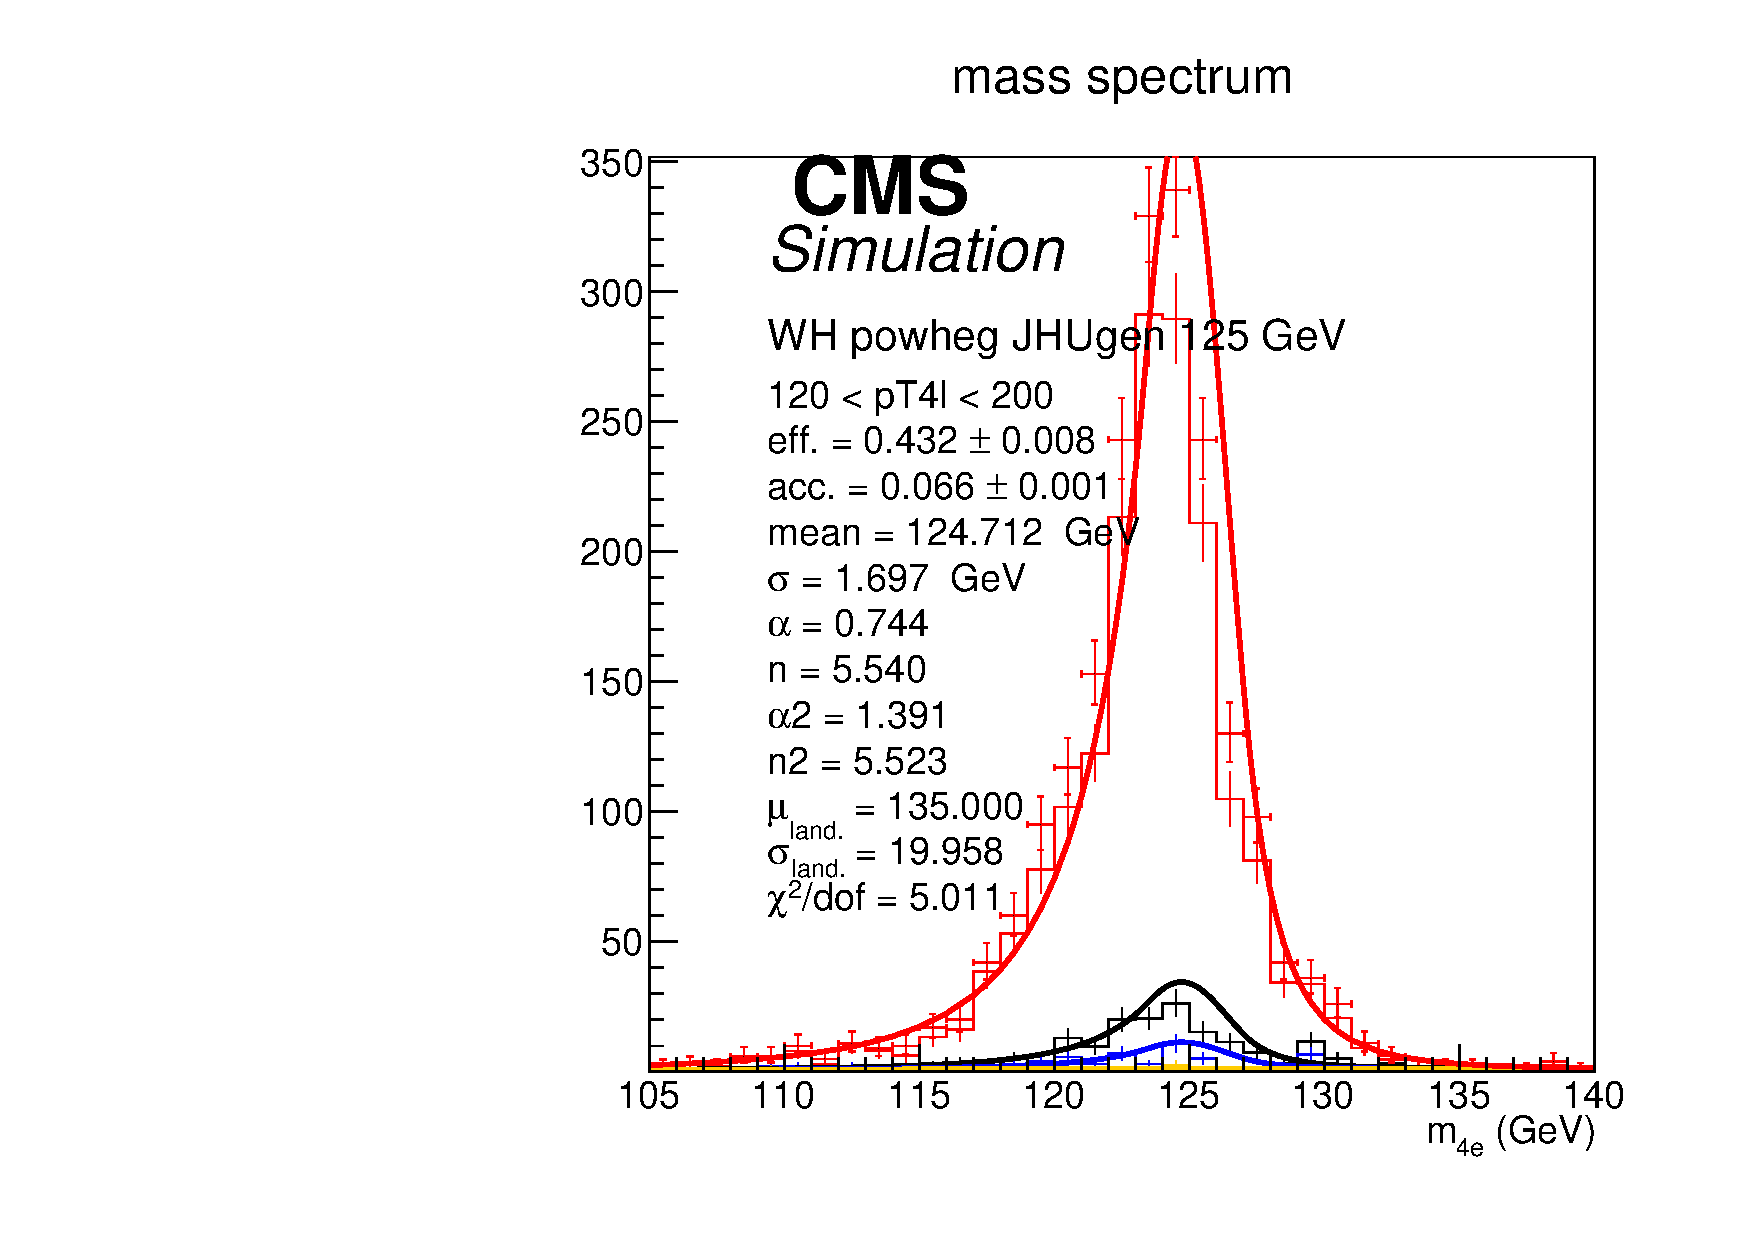
\includegraphics[width=0.3\textwidth,angle=0]{Figures/Appendix//WH_powheg_JHUgen_125_4e_pT4l_genbin5_recobin5_effs_genWeight*pileupWeight*dataMCWeight.pdf}
      \label{fig:sigfits-pT4l-WH-powheg15-JHUgen-125-maintext:f}
    } \\
    \subfigure[$200.0 < \pt(\mathrm{H}) < 13000.0$]{
      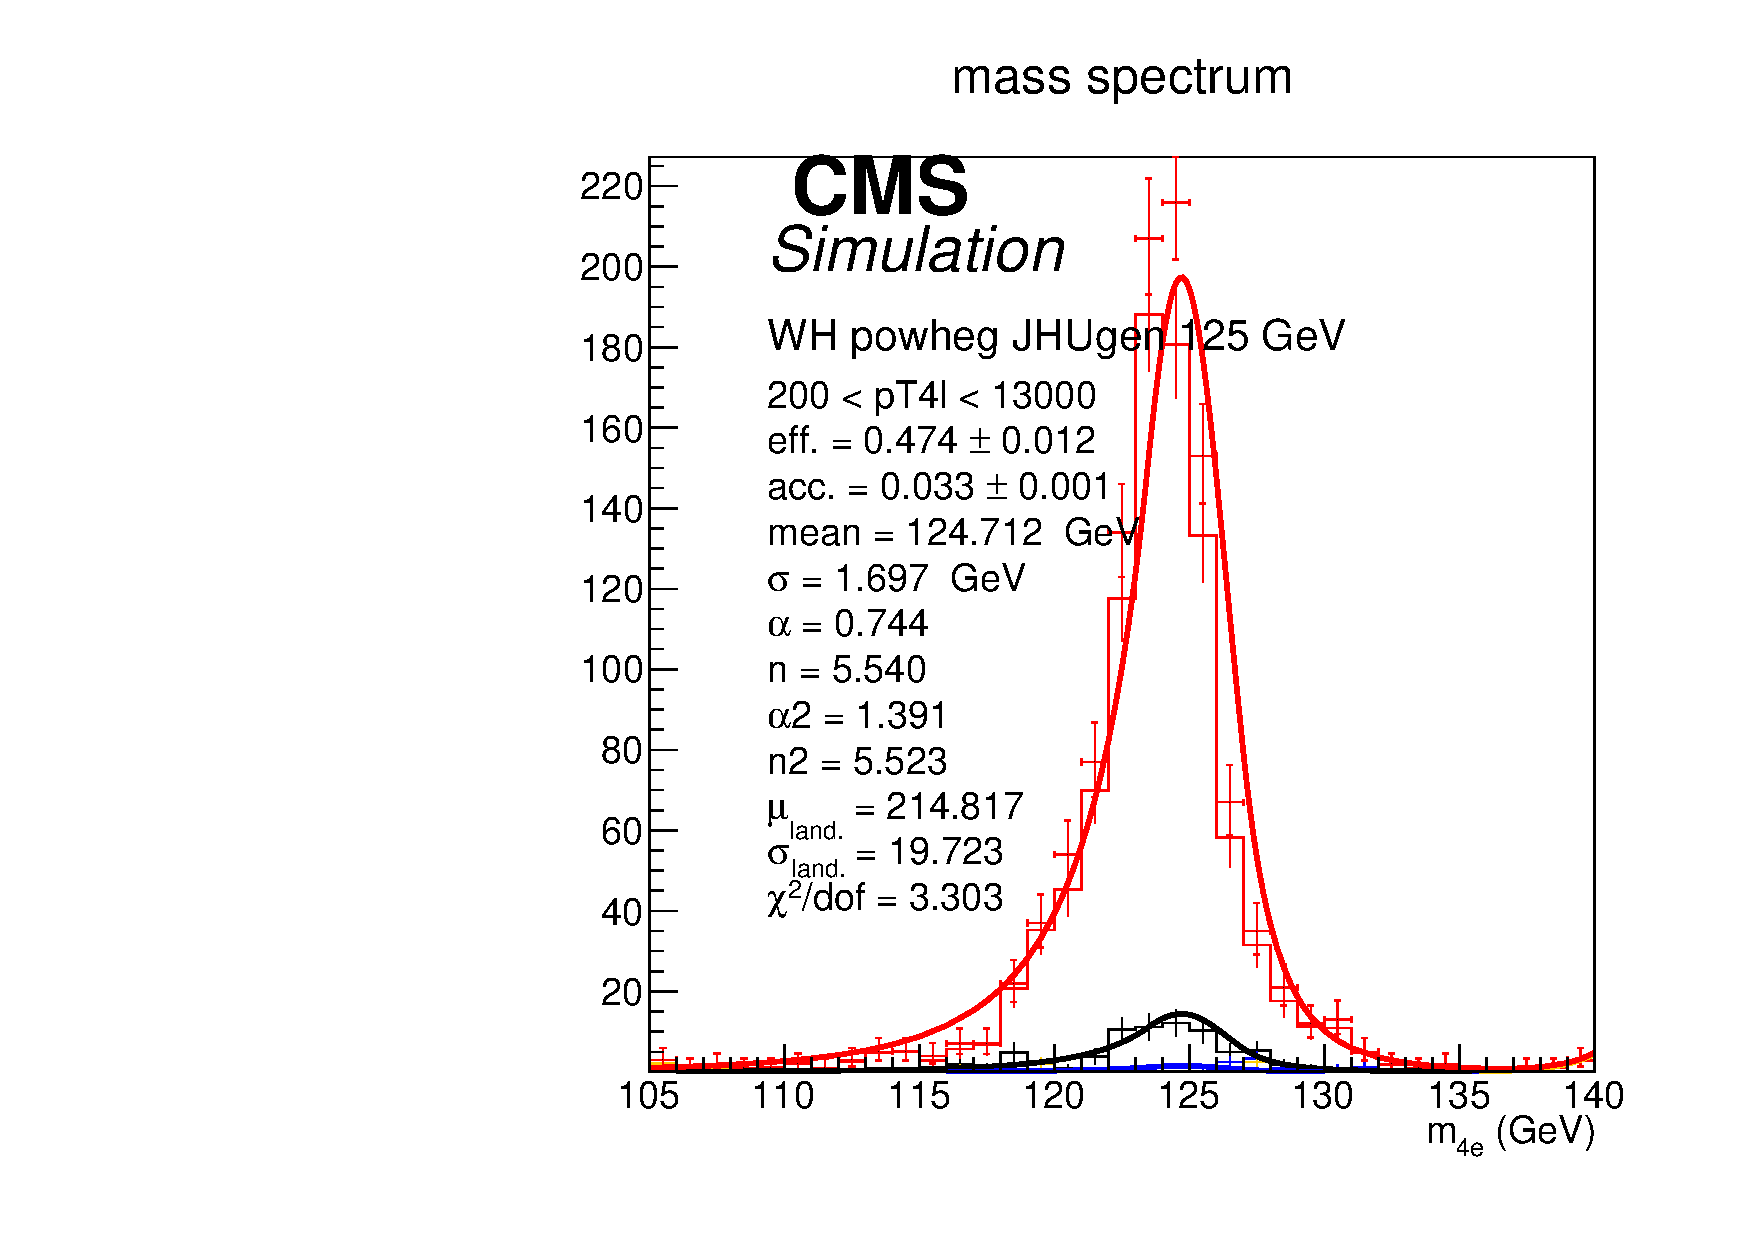
\includegraphics[width=0.3\textwidth,angle=0]{Figures/Appendix//WH_powheg_JHUgen_125_4e_pT4l_genbin6_recobin6_effs_genWeight*pileupWeight*dataMCWeight.pdf}
      \label{fig:sigfits-pT4l-WH-powheg15-JHUgen-125-maintext:g}
    }
    \\
    \caption{ Example signal shapes at reconstruction level for a resonance of m(4$\ell$) in $4e$ final state for the $WH$ production mode from {\sc powheg+JHUGen} in different bins of $\pt(\mathrm{H})$. The black curve represents events which do not pass the fiducial volume selection. The curve has no effect on the result.
    }
  \label{fig:sigfits-pT4l-WH-powheg15-JHUgen-125-maintext}
 \end{center}
\end{figure} \clearpage


\begin{figure}[htb]
  \begin{center}
    \subfigure[$0.0 < \pt(\mathrm{H}) < 15.0 $]{
      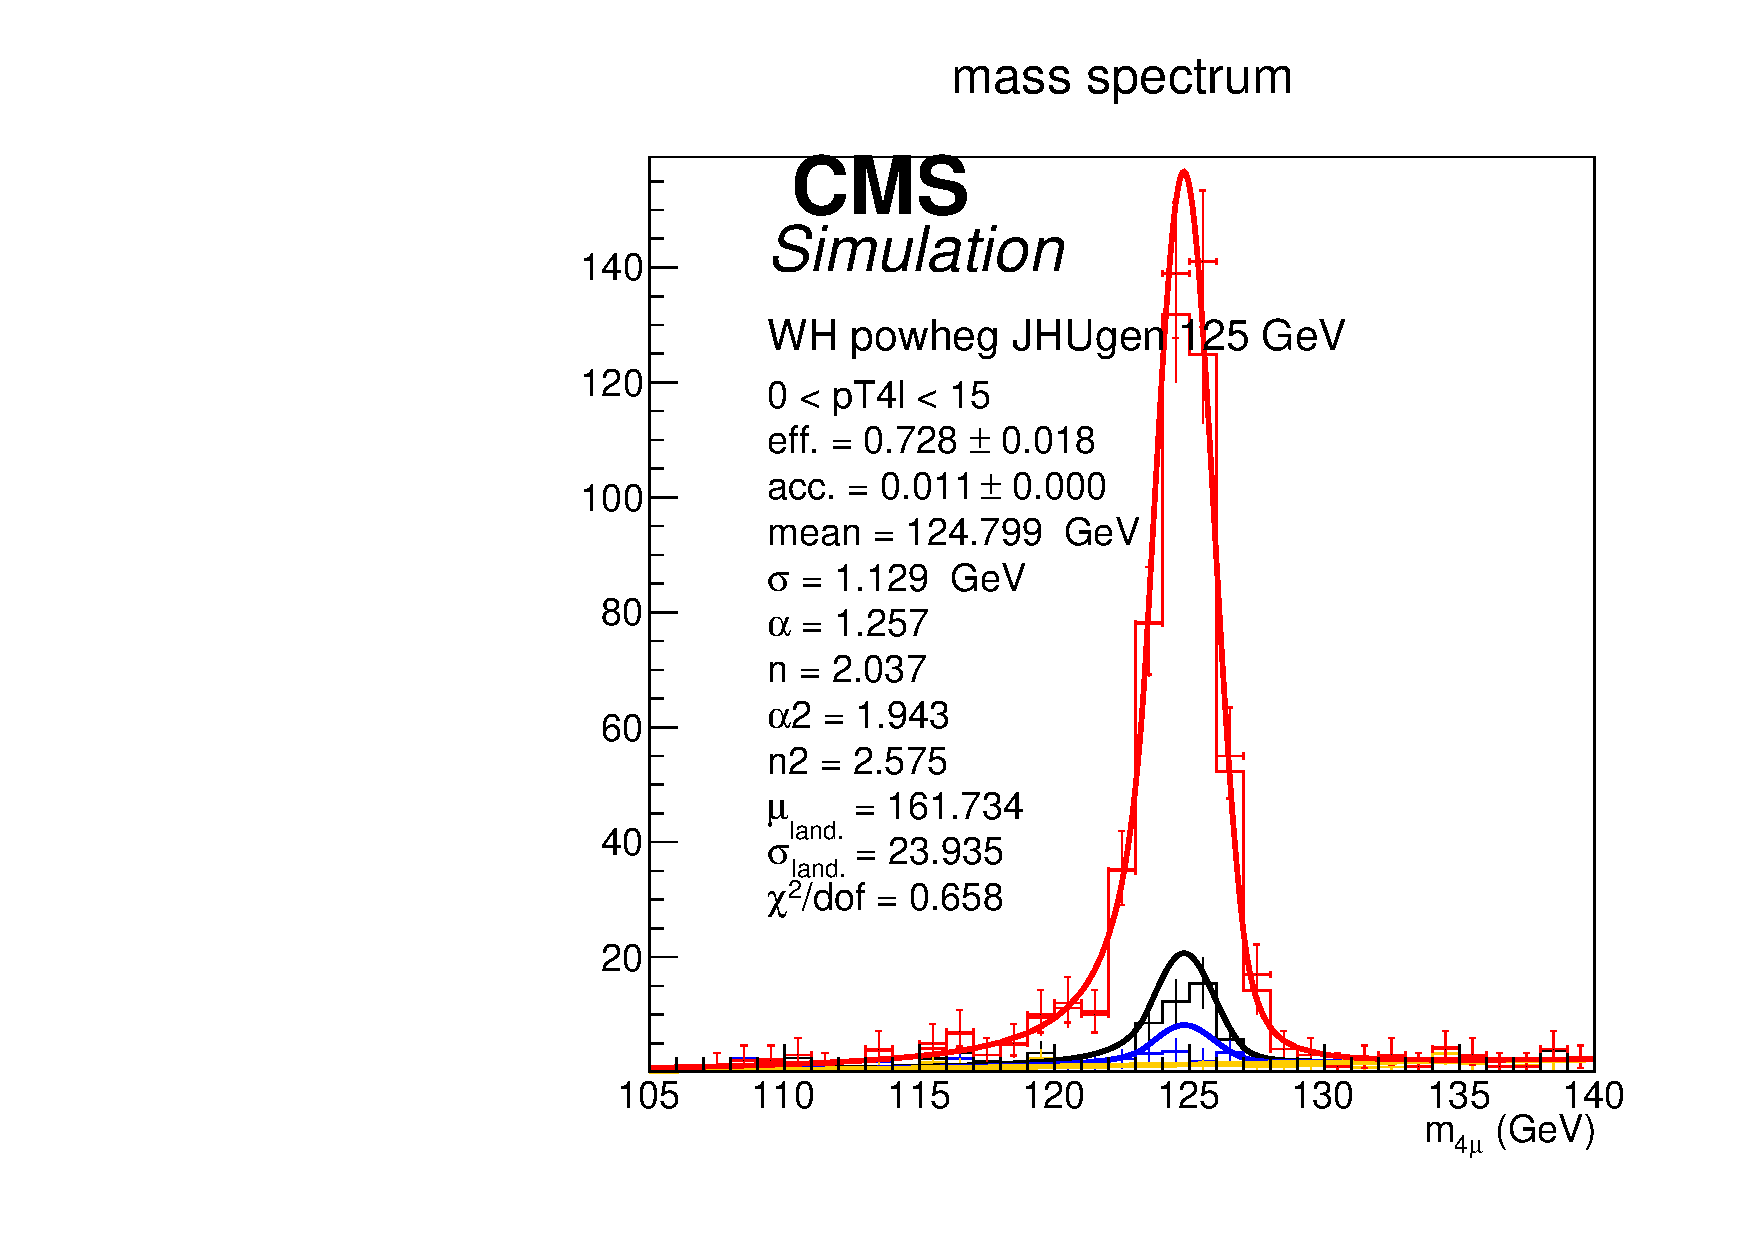
\includegraphics[width=0.3\textwidth,angle=0]{Figures/Appendix//WH_powheg_JHUgen_125_4mu_pT4l_genbin0_recobin0_effs_genWeight*pileupWeight*dataMCWeight.pdf}
      \label{fig:sigfits-pT4l-WH-powheg15-JHUgen-125-maintext:a}
    }
    \subfigure[$15.0 < \pt(\mathrm{H}) < 30.0$]{
      \includegraphics[width=0.3\textwidth,angle=0]{Figures/Appendix//WH_powheg_JHUgen_125_4mu_pT4l_genbin1_recobin1_effs_genWeight*pileupWeight*dataMCWeight.pdf}
      \label{fig:sigfits-pT4l-WH-powheg15-JHUgen-125-maintext:b}
    }
   \subfigure[$30.0 < \pt(\mathrm{H}) < 45.0$]{
      \includegraphics[width=0.3\textwidth,angle=0]{Figures/Appendix//WH_powheg_JHUgen_125_4mu_pT4l_genbin2_recobin2_effs_genWeight*pileupWeight*dataMCWeight.pdf}
      \label{fig:sigfits-pT4l-WH-powheg15-JHUgen-125-maintext:c}
    }  \\
    \subfigure[$45.0 < \pt(\mathrm{H}) < 80.0$]{
      \includegraphics[width=0.3\textwidth,angle=0]{Figures/Appendix//WH_powheg_JHUgen_125_4mu_pT4l_genbin3_recobin3_effs_genWeight*pileupWeight*dataMCWeight.pdf}
      \label{fig:sigfits-pT4l-WH-powheg15-JHUgen-125-maintext:d}
    }
    \subfigure[$80.0 < \pt(\mathrm{H}) < 120.0$]{
      \includegraphics[width=0.3\textwidth,angle=0]{Figures/Appendix//WH_powheg_JHUgen_125_4mu_pT4l_genbin4_recobin4_effs_genWeight*pileupWeight*dataMCWeight.pdf}
      \label{fig:sigfits-pT4l-WH-powheg15-JHUgen-125-maintext:e}
    }
    \subfigure[$120.0 < \pt(\mathrm{H}) < 200.0$]{
      \includegraphics[width=0.3\textwidth,angle=0]{Figures/Appendix//WH_powheg_JHUgen_125_4mu_pT4l_genbin5_recobin5_effs_genWeight*pileupWeight*dataMCWeight.pdf}
      \label{fig:sigfits-pT4l-WH-powheg15-JHUgen-125-maintext:f}
    } \\
    \subfigure[$200.0 < \pt(\mathrm{H}) < 13000.0$]{
      \includegraphics[width=0.3\textwidth,angle=0]{Figures/Appendix//WH_powheg_JHUgen_125_4mu_pT4l_genbin6_recobin6_effs_genWeight*pileupWeight*dataMCWeight.pdf}
      \label{fig:sigfits-pT4l-WH-powheg15-JHUgen-125-maintext:g}
    }
    \\
    \caption{ Example signal shapes at reconstruction level for a resonance of m(4$\ell$) in $4\mu$ final state for the $gg\rightarrow \mathrm{H}$ production mode from {\sc powheg+JHUGen} in different bins of $\pt(\mathrm{H})$. The black curve represents events which do not pass the fiducial volume selection. The curve has no effect on the result.
    }
  \label{fig:sigfits-pT4l-WH-powheg15-JHUgen-125-maintext}
 \end{center}
\end{figure} \clearpage

\begin{figure}[htb]
  \begin{center}
    \subfigure[$0.0 < \pt(\mathrm{H}) < 15.0 $]{
      \includegraphics[width=0.3\textwidth,angle=0]{Figures/Appendix//ZH_powheg_JHUgen_125_2e2mu_pT4l_genbin0_recobin0_effs_genWeight*pileupWeight*dataMCWeight.pdf}
      \label{fig:sigfits-pT4l-ZH-powheg15-JHUgen-125-maintext:a}
    }
    \subfigure[$15.0 < \pt(\mathrm{H}) < 30.0$]{
      \includegraphics[width=0.3\textwidth,angle=0]{Figures/Appendix//ZH_powheg_JHUgen_125_2e2mu_pT4l_genbin1_recobin1_effs_genWeight*pileupWeight*dataMCWeight.pdf}
      \label{fig:sigfits-pT4l-ZH-powheg15-JHUgen-125-maintext:b}
    }
   \subfigure[$30.0 < \pt(\mathrm{H}) < 45.0$]{
      \includegraphics[width=0.3\textwidth,angle=0]{Figures/Appendix//ZH_powheg_JHUgen_125_2e2mu_pT4l_genbin2_recobin2_effs_genWeight*pileupWeight*dataMCWeight.pdf}
      \label{fig:sigfits-pT4l-ZH-powheg15-JHUgen-125-maintext:c}
    }  \\
    \subfigure[$45.0 < \pt(\mathrm{H}) < 80.0$]{
      \includegraphics[width=0.3\textwidth,angle=0]{Figures/Appendix//ZH_powheg_JHUgen_125_2e2mu_pT4l_genbin3_recobin3_effs_genWeight*pileupWeight*dataMCWeight.pdf}
      \label{fig:sigfits-pT4l-ZH-powheg15-JHUgen-125-maintext:d}
    }
    \subfigure[$80.0 < \pt(\mathrm{H}) < 120.0$]{
      \includegraphics[width=0.3\textwidth,angle=0]{Figures/Appendix//ZH_powheg_JHUgen_125_2e2mu_pT4l_genbin4_recobin4_effs_genWeight*pileupWeight*dataMCWeight.pdf}
      \label{fig:sigfits-pT4l-ZH-powheg15-JHUgen-125-maintext:e}
    }
    \subfigure[$120.0 < \pt(\mathrm{H}) < 200.0$]{
      \includegraphics[width=0.3\textwidth,angle=0]{Figures/Appendix//ZH_powheg_JHUgen_125_2e2mu_pT4l_genbin5_recobin5_effs_genWeight*pileupWeight*dataMCWeight.pdf}
      \label{fig:sigfits-pT4l-ZH-powheg15-JHUgen-125-maintext:f}
    } \\
    \subfigure[$200.0 < \pt(\mathrm{H}) < 13000.0$]{
      \includegraphics[width=0.3\textwidth,angle=0]{Figures/Appendix//ZH_powheg_JHUgen_125_2e2mu_pT4l_genbin6_recobin6_effs_genWeight*pileupWeight*dataMCWeight.pdf}
      \label{fig:sigfits-pT4l-ZH-powheg15-JHUgen-125-maintext:g}
    }
    \\
    \caption{ Example signal shapes at reconstruction level for a resonance of m(4$\ell$) in $2e2\mu$ final state for the $ZH$ production mode from {\sc powheg+JHUGen} in different bins of $\pt(\mathrm{H})$. The black curve represents events which do not pass the fiducial volume selection. The curve has no effect on the result.
    }
  \label{fig:sigfits-pT4l-ZH-powheg15-JHUgen-125-maintext}
 \end{center}
\end{figure} \clearpage

\begin{figure}[htb]
  \begin{center}
    \subfigure[$0.0 < \pt(\mathrm{H}) < 15.0 $]{
      \includegraphics[width=0.3\textwidth,angle=0]{Figures/Appendix//ZH_powheg_JHUgen_125_4e_pT4l_genbin0_recobin0_effs_genWeight*pileupWeight*dataMCWeight.pdf}
      \label{fig:sigfits-pT4l-ZH-powheg15-JHUgen-125-maintext:a}
    }
    \subfigure[$15.0 < \pt(\mathrm{H}) < 30.0$]{
      \includegraphics[width=0.3\textwidth,angle=0]{Figures/Appendix//ZH_powheg_JHUgen_125_4e_pT4l_genbin1_recobin1_effs_genWeight*pileupWeight*dataMCWeight.pdf}
      \label{fig:sigfits-pT4l-ZH-powheg15-JHUgen-125-maintext:b}
    }
   \subfigure[$30.0 < \pt(\mathrm{H}) < 45.0$]{
      \includegraphics[width=0.3\textwidth,angle=0]{Figures/Appendix//ZH_powheg_JHUgen_125_4e_pT4l_genbin2_recobin2_effs_genWeight*pileupWeight*dataMCWeight.pdf}
      \label{fig:sigfits-pT4l-ZH-powheg15-JHUgen-125-maintext:c}
    }  \\
    \subfigure[$45.0 < \pt(\mathrm{H}) < 80.0$]{
      \includegraphics[width=0.3\textwidth,angle=0]{Figures/Appendix//ZH_powheg_JHUgen_125_4e_pT4l_genbin3_recobin3_effs_genWeight*pileupWeight*dataMCWeight.pdf}
      \label{fig:sigfits-pT4l-ZH-powheg15-JHUgen-125-maintext:d}
    }
    \subfigure[$80.0 < \pt(\mathrm{H}) < 120.0$]{
      \includegraphics[width=0.3\textwidth,angle=0]{Figures/Appendix//ZH_powheg_JHUgen_125_4e_pT4l_genbin4_recobin4_effs_genWeight*pileupWeight*dataMCWeight.pdf}
      \label{fig:sigfits-pT4l-ZH-powheg15-JHUgen-125-maintext:e}
    }
    \subfigure[$120.0 < \pt(\mathrm{H}) < 200.0$]{
      \includegraphics[width=0.3\textwidth,angle=0]{Figures/Appendix//ZH_powheg_JHUgen_125_4e_pT4l_genbin5_recobin5_effs_genWeight*pileupWeight*dataMCWeight.pdf}
      \label{fig:sigfits-pT4l-ZH-powheg15-JHUgen-125-maintext:f}
    } \\
    \subfigure[$200.0 < \pt(\mathrm{H}) < 13000.0$]{
      \includegraphics[width=0.3\textwidth,angle=0]{Figures/Appendix//ZH_powheg_JHUgen_125_4e_pT4l_genbin6_recobin6_effs_genWeight*pileupWeight*dataMCWeight.pdf}
      \label{fig:sigfits-pT4l-ZH-powheg15-JHUgen-125-maintext:g}
    }
    \\
    \caption{ Example signal shapes at reconstruction level for a resonance of m(4$\ell$) in $4e$ final state for the $ZH$ production mode from {\sc powheg+JHUGen} in different bins of $\pt(\mathrm{H})$. The black curve represents events which do not pass the fiducial volume selection. The curve has no effect on the result.
    }
  \label{fig:sigfits-pT4l-ZH-powheg15-JHUgen-125-maintext}
 \end{center}
\end{figure} \clearpage

\begin{figure}[htb]
  \begin{center}
    \subfigure[$0.0 < \pt(\mathrm{H}) < 15.0 $]{
      \includegraphics[width=0.3\textwidth,angle=0]{Figures/Appendix//ZH_powheg_JHUgen_125_4mu_pT4l_genbin0_recobin0_effs_genWeight*pileupWeight*dataMCWeight.pdf}
      \label{fig:sigfits-pT4l-ZH-powheg15-JHUgen-125-maintext:a}
    }
    \subfigure[$15.0 < \pt(\mathrm{H}) < 30.0$]{
      \includegraphics[width=0.3\textwidth,angle=0]{Figures/Appendix//ZH_powheg_JHUgen_125_4mu_pT4l_genbin1_recobin1_effs_genWeight*pileupWeight*dataMCWeight.pdf}
      \label{fig:sigfits-pT4l-ZH-powheg15-JHUgen-125-maintext:b}
    }
   \subfigure[$30.0 < \pt(\mathrm{H}) < 45.0$]{
      \includegraphics[width=0.3\textwidth,angle=0]{Figures/Appendix//ZH_powheg_JHUgen_125_4mu_pT4l_genbin2_recobin2_effs_genWeight*pileupWeight*dataMCWeight.pdf}
      \label{fig:sigfits-pT4l-ZH-powheg15-JHUgen-125-maintext:c}
    }  \\
    \subfigure[$45.0 < \pt(\mathrm{H}) < 80.0$]{
      \includegraphics[width=0.3\textwidth,angle=0]{Figures/Appendix//ZH_powheg_JHUgen_125_4mu_pT4l_genbin3_recobin3_effs_genWeight*pileupWeight*dataMCWeight.pdf}
      \label{fig:sigfits-pT4l-ZH-powheg15-JHUgen-125-maintext:d}
    }
    \subfigure[$80.0 < \pt(\mathrm{H}) < 120.0$]{
      \includegraphics[width=0.3\textwidth,angle=0]{Figures/Appendix//ZH_powheg_JHUgen_125_4mu_pT4l_genbin4_recobin4_effs_genWeight*pileupWeight*dataMCWeight.pdf}
      \label{fig:sigfits-pT4l-ZH-powheg15-JHUgen-125-maintext:e}
    }
    \subfigure[$120.0 < \pt(\mathrm{H}) < 200.0$]{
      \includegraphics[width=0.3\textwidth,angle=0]{Figures/Appendix//ZH_powheg_JHUgen_125_4mu_pT4l_genbin5_recobin5_effs_genWeight*pileupWeight*dataMCWeight.pdf}
      \label{fig:sigfits-pT4l-ZH-powheg15-JHUgen-125-maintext:f}
    } \\
    \subfigure[$200.0 < \pt(\mathrm{H}) < 13000.0$]{
      \includegraphics[width=0.3\textwidth,angle=0]{Figures/Appendix//ZH_powheg_JHUgen_125_4mu_pT4l_genbin6_recobin6_effs_genWeight*pileupWeight*dataMCWeight.pdf}
      \label{fig:sigfits-pT4l-ZH-powheg15-JHUgen-125-maintext:g}
    }
    \\
    \caption{ Example signal shapes at reconstruction level for a resonance of m(4$\ell$) in $4\mu$ final state for the $ZH$ production mode from {\sc powheg+JHUGen} in different bins of $\pt(\mathrm{H})$. The black curve represents events which do not pass the fiducial volume selection. The curve has no effect on the result.
    }
  \label{fig:sigfits-pT4l-ZH-powheg15-JHUgen-125-maintext}
 \end{center}
\end{figure} \clearpage

%%%%%%%%%%%%%%%%%%%%%%%%%%%%%%%%%%%%%%%%%%%%%%%%%%%%  ttH
\begin{figure}[htb]
  \begin{center}
    \subfigure[$0.0 < \pt(\mathrm{H}) < 15.0 $]{
      \includegraphics[width=0.3\textwidth,angle=0]{Figures/Appendix//ttH_powheg_JHUgen_125_2e2mu_pT4l_genbin0_recobin0_effs_genWeight*pileupWeight*dataMCWeight.pdf}
      \label{fig:sigfits-pT4l-ttH-powheg15-JHUgen-125-maintext:a}
    }
    \subfigure[$15.0 < \pt(\mathrm{H}) < 30.0$]{
      \includegraphics[width=0.3\textwidth,angle=0]{Figures/Appendix//ttH_powheg_JHUgen_125_2e2mu_pT4l_genbin1_recobin1_effs_genWeight*pileupWeight*dataMCWeight.pdf}
      \label{fig:sigfits-pT4l-ttH-powheg15-JHUgen-125-maintext:b}
    }
   \subfigure[$30.0 < \pt(\mathrm{H}) < 45.0$]{
      \includegraphics[width=0.3\textwidth,angle=0]{Figures/Appendix//ttH_powheg_JHUgen_125_2e2mu_pT4l_genbin2_recobin2_effs_genWeight*pileupWeight*dataMCWeight.pdf}
      \label{fig:sigfits-pT4l-ttH-powheg15-JHUgen-125-maintext:c}
    }  \\
    \subfigure[$45.0 < \pt(\mathrm{H}) < 80.0$]{
      \includegraphics[width=0.3\textwidth,angle=0]{Figures/Appendix//ttH_powheg_JHUgen_125_2e2mu_pT4l_genbin3_recobin3_effs_genWeight*pileupWeight*dataMCWeight.pdf}
      \label{fig:sigfits-pT4l-ttH-powheg15-JHUgen-125-maintext:d}
    }
    \subfigure[$80.0 < \pt(\mathrm{H}) < 120.0$]{
      \includegraphics[width=0.3\textwidth,angle=0]{Figures/Appendix//ttH_powheg_JHUgen_125_2e2mu_pT4l_genbin4_recobin4_effs_genWeight*pileupWeight*dataMCWeight.pdf}
      \label{fig:sigfits-pT4l-ttH-powheg15-JHUgen-125-maintext:e}
    }
    \subfigure[$120.0 < \pt(\mathrm{H}) < 200.0$]{
      \includegraphics[width=0.3\textwidth,angle=0]{Figures/Appendix//ttH_powheg_JHUgen_125_2e2mu_pT4l_genbin5_recobin5_effs_genWeight*pileupWeight*dataMCWeight.pdf}
      \label{fig:sigfits-pT4l-ttH-powheg15-JHUgen-125-maintext:f}
    } \\
    \subfigure[$200.0 < \pt(\mathrm{H}) < 13000.0$]{
      \includegraphics[width=0.3\textwidth,angle=0]{Figures/Appendix//ttH_powheg_JHUgen_125_2e2mu_pT4l_genbin6_recobin6_effs_genWeight*pileupWeight*dataMCWeight.pdf}
      \label{fig:sigfits-pT4l-ttH-powheg15-JHUgen-125-maintext:g}
    }
    \\
    \caption{ Example signal shapes at reconstruction level for a resonance of m(4$\ell$) in $2e2\mu$ final state for the $ttH$ production mode from {\sc powheg+JHUGen} in different bins of $\pt(\mathrm{H})$. The black curve represents events which do not pass the fiducial volume selection. The curve has no effect on the result.
    }
  \label{fig:sigfits-pT4l-ttH-powheg15-JHUgen-125-maintext}
 \end{center}
\end{figure} \clearpage

\begin{figure}[htb]
  \begin{center}
    \subfigure[$0.0 < \pt(\mathrm{H}) < 15.0 $]{
      \includegraphics[width=0.3\textwidth,angle=0]{Figures/Appendix//ggH_powheg_JHUgen_125_4e_pT4l_genbin0_recobin0_effs_genWeight*pileupWeight*dataMCWeight.pdf}
      \label{fig:sigfits-pT4l-ggH-powheg15-JHUgen-125-maintext:a}
    }
    \subfigure[$15.0 < \pt(\mathrm{H}) < 30.0$]{
      \includegraphics[width=0.3\textwidth,angle=0]{Figures/Appendix//ggH_powheg_JHUgen_125_4e_pT4l_genbin1_recobin1_effs_genWeight*pileupWeight*dataMCWeight.pdf}
      \label{fig:sigfits-pT4l-ggH-powheg15-JHUgen-125-maintext:b}
    }
   \subfigure[$30.0 < \pt(\mathrm{H}) < 45.0$]{
      \includegraphics[width=0.3\textwidth,angle=0]{Figures/Appendix//ggH_powheg_JHUgen_125_4e_pT4l_genbin2_recobin2_effs_genWeight*pileupWeight*dataMCWeight.pdf}
      \label{fig:sigfits-pT4l-ggH-powheg15-JHUgen-125-maintext:c}
    }  \\
    \subfigure[$45.0 < \pt(\mathrm{H}) < 80.0$]{
      \includegraphics[width=0.3\textwidth,angle=0]{Figures/Appendix//ggH_powheg_JHUgen_125_4e_pT4l_genbin3_recobin3_effs_genWeight*pileupWeight*dataMCWeight.pdf}
      \label{fig:sigfits-pT4l-ggH-powheg15-JHUgen-125-maintext:d}
    }
    \subfigure[$80.0 < \pt(\mathrm{H}) < 120.0$]{
      \includegraphics[width=0.3\textwidth,angle=0]{Figures/Appendix//ggH_powheg_JHUgen_125_4e_pT4l_genbin4_recobin4_effs_genWeight*pileupWeight*dataMCWeight.pdf}
      \label{fig:sigfits-pT4l-ggH-powheg15-JHUgen-125-maintext:e}
    }
    \subfigure[$120.0 < \pt(\mathrm{H}) < 200.0$]{
      \includegraphics[width=0.3\textwidth,angle=0]{Figures/Appendix//ggH_powheg_JHUgen_125_4e_pT4l_genbin5_recobin5_effs_genWeight*pileupWeight*dataMCWeight.pdf}
      \label{fig:sigfits-pT4l-ggH-powheg15-JHUgen-125-maintext:f}
    } \\
    \subfigure[$200.0 < \pt(\mathrm{H}) < 13000.0$]{
      \includegraphics[width=0.3\textwidth,angle=0]{Figures/Appendix//ggH_powheg_JHUgen_125_4e_pT4l_genbin6_recobin6_effs_genWeight*pileupWeight*dataMCWeight.pdf}
      \label{fig:sigfits-pT4l-ggH-powheg15-JHUgen-125-maintext:g}
    }
    \\
    \caption{ Example signal shapes at reconstruction level for a resonance of m(4$\ell$) in $4e$ final state for the $ttH$ production mode from {\sc powheg+JHUGen} in different bins of $\pt(\mathrm{H})$. The black curve represents events which do not pass the fiducial volume selection. The curve has no effect on the result.
    }
  \label{fig:sigfits-pT4l-ggH-powheg15-JHUgen-125-maintext}
 \end{center}
\end{figure} \clearpage



\begin{figure}[htb]
  \begin{center}
    \subfigure[$0.0 < \pt(\mathrm{H}) < 15.0 $]{
      \includegraphics[width=0.3\textwidth,angle=0]{Figures/Appendix//ttH_powheg_JHUgen_125_4mu_pT4l_genbin0_recobin0_effs_genWeight*pileupWeight*dataMCWeight.pdf}
      \label{fig:sigfits-pT4l-ttH-powheg15-JHUgen-125-maintext:a}
    }
    \subfigure[$15.0 < \pt(\mathrm{H}) < 30.0$]{
      \includegraphics[width=0.3\textwidth,angle=0]{Figures/Appendix//ttH_powheg_JHUgen_125_4mu_pT4l_genbin1_recobin1_effs_genWeight*pileupWeight*dataMCWeight.pdf}
      \label{fig:sigfits-pT4l-ttH-powheg15-JHUgen-125-maintext:b}
    }
   \subfigure[$30.0 < \pt(\mathrm{H}) < 45.0$]{
      \includegraphics[width=0.3\textwidth,angle=0]{Figures/Appendix//ttH_powheg_JHUgen_125_4mu_pT4l_genbin2_recobin2_effs_genWeight*pileupWeight*dataMCWeight.pdf}
      \label{fig:sigfits-pT4l-ttH-powheg15-JHUgen-125-maintext:c}
    }  \\
    \subfigure[$45.0 < \pt(\mathrm{H}) < 80.0$]{
      \includegraphics[width=0.3\textwidth,angle=0]{Figures/Appendix//ttH_powheg_JHUgen_125_4mu_pT4l_genbin3_recobin3_effs_genWeight*pileupWeight*dataMCWeight.pdf}
      \label{fig:sigfits-pT4l-ttH-powheg15-JHUgen-125-maintext:d}
    }
    \subfigure[$80.0 < \pt(\mathrm{H}) < 120.0$]{
      \includegraphics[width=0.3\textwidth,angle=0]{Figures/Appendix//ttH_powheg_JHUgen_125_4mu_pT4l_genbin4_recobin4_effs_genWeight*pileupWeight*dataMCWeight.pdf}
      \label{fig:sigfits-pT4l-ttH-powheg15-JHUgen-125-maintext:e}
    }
    \subfigure[$120.0 < \pt(\mathrm{H}) < 200.0$]{
      \includegraphics[width=0.3\textwidth,angle=0]{Figures/Appendix//ttH_powheg_JHUgen_125_4mu_pT4l_genbin5_recobin5_effs_genWeight*pileupWeight*dataMCWeight.pdf}
      \label{fig:sigfits-pT4l-ttH-powheg15-JHUgen-125-maintext:f}
    } \\
    \subfigure[$200.0 < \pt(\mathrm{H}) < 13000.0$]{
      \includegraphics[width=0.3\textwidth,angle=0]{Figures/Appendix//ttH_powheg_JHUgen_125_4mu_pT4l_genbin6_recobin6_effs_genWeight*pileupWeight*dataMCWeight.pdf}
      \label{fig:sigfits-pT4l-ttH-powheg15-JHUgen-125-maintext:g}
    }
    \\
    \caption{ Example signal shapes at reconstruction level for a resonance of m(4$\ell$) in $4\mu$ final state for the $ttH$ production mode from {\sc powheg+JHUGen} in different bins of $\pt(\mathrm{H})$. The black curve represents events which do not pass the fiducial volume selection. The curve has no effect on the result.
    }
  \label{fig:sigfits-pT4l-ttH-powheg15-JHUgen-125-maintext}
 \end{center}
\end{figure} \clearpage


%%%%%%%%%%%%%%%%%%%%%%%%%%%%%  2D response matrices

\begin{figure}[!h!tb]
  \begin{center}
    \subfigure[$gg\rightarrow$H ({\sc powheg+JHUgen})]{
    \includegraphics[width=0.30\textwidth,angle=0]{Figures/Appendix//eff2d_ggH_powheg_JHUgen_125_pT4l_4e.pdf}
    \label{fig:eff-pT4l-4e:a}
    }
%    \subfigure[$gg\rightarrow$H ({\sc minloHJJ})]{
%    \includegraphics[width=0.30\textwidth,angle=0]{Figures/Appendix//eff2d_ggH_minloHJJ_125_pT4l_4e.pdf}
%    \label{fig:eff-pT4l-4e:b}
%    } \\
    \subfigure[VBF ({\sc powheg})]{
    \includegraphics[width=0.30\textwidth,angle=0]{Figures/Appendix//eff2d_VBF_powheg_JHUgen_125_pT4l_4e.pdf}
    \label{fig:eff-pT4l-4e:c}
    }
    \subfigure[WH ({\sc pythia})]{
    \includegraphics[width=0.30\textwidth,angle=0]{Figures/Appendix//eff2d_WH_powheg_JHUgen_125_pT4l_4e.pdf}
    \label{fig:eff-pT4l-4e:d}
    } \\
    \subfigure[ZH ({\sc pythia})]{
    \includegraphics[width=0.30\textwidth,angle=0]{Figures/Appendix//eff2d_ZH_powheg_JHUgen_125_pT4l_4e.pdf}
    \label{fig:eff-pT4l-4e:e}
    }
    \subfigure[ttH ({\sc pythia})]{
    \includegraphics[width=0.30\textwidth,angle=0]{Figures/Appendix//eff2d_ttH_powheg_JHUgen_125_pT4l_4e.pdf}
    \label{fig:eff-pT4l-4e:f}
    } 
    \caption{ Efficiency matrices for  $\pt({\rm H})$ for different SM production modes in the $4e$ final state. }
    \label{fig:eff-pT4l-4e}
  \end{center}
\end{figure} \clearpage


\begin{figure}[!h!tb]
  \begin{center}
    \subfigure[$gg\rightarrow$H ({\sc powheg+JHUgen})]{
    \includegraphics[width=0.30\textwidth,angle=0]{Figures/Appendix//eff2d_ggH_powheg_JHUgen_125_pT4l_4mu.pdf}
    \label{fig:eff-pT4l-4mu:a}
    }
%    \subfigure[$\Pg\Pg\rightarrow$H ({\sc minloHJJ})]{
%    \includegraphics[width=0.30\textwidth,angle=0]{Figures/Appendix//eff2d_ggH_minloHJJ_125_pT4l_4mu.pdf}
%    \label{fig:eff-pT4l-4mu:b}
%    } \\
    \subfigure[VBF ({\sc powheg})]{
    \includegraphics[width=0.30\textwidth,angle=0]{Figures/Appendix//eff2d_VBF_powheg_JHUgen_125_pT4l_4mu.pdf}
    \label{fig:eff-pT4l-4mu:c}
    }
    \subfigure[WH ({\sc pythia})]{
    \includegraphics[width=0.30\textwidth,angle=0]{Figures/Appendix//eff2d_WH_powheg_JHUgen_125_pT4l_4mu.pdf}
    \label{fig:eff-pT4l-4mu:d}
    } \\
    \subfigure[ZH ({\sc pythia})]{
    \includegraphics[width=0.30\textwidth,angle=0]{Figures/Appendix//eff2d_ZH_powheg_JHUgen_125_pT4l_4mu.pdf}
    \label{fig:eff-pT4l-4mu:e}
    }
    \subfigure[ttH ({\sc pythia})]{
    \includegraphics[width=0.30\textwidth,angle=0]{Figures/Appendix//eff2d_ttH_powheg_JHUgen_125_pT4l_4mu.pdf}
    \label{fig:eff-pT4l-4mu:f}
    } 
    \caption{ Efficiency matrices for  $\pt({\rm H})$ for different SM production modes in the $4\mu$ final state. }
    \label{fig:eff-pT4l-4mu}
  \end{center}
\end{figure} \clearpage

\begin{figure}[!h!tb]
  \begin{center}
    \subfigure[$gg\rightarrow$H ({\sc powheg+JHUgen})]{
    \includegraphics[width=0.30\textwidth,angle=0]{Figures/Appendix//eff2d_ggH_powheg_JHUgen_125_pT4l_2e2mu.pdf}
    \label{fig:eff-pT4l-2e2mu:a}
    }
%    \subfigure[$\Pg\Pg\rightarrow$H ({\sc minloHJJ})]{
%    \includegraphics[width=0.30\textwidth,angle=0]{Figures/Appendix//eff2d_ggH_minloHJJ_125_pT4l_2e2mu.pdf}
%    \label{fig:eff-pT4l-2e2mu:b}
%    } \\
    \subfigure[VBF ({\sc powheg})]{
    \includegraphics[width=0.30\textwidth,angle=0]{Figures/Appendix//eff2d_VBF_powheg_JHUgen_125_pT4l_2e2mu.pdf}
    \label{fig:eff-pT4l-2e2mu:c}
    }
    \subfigure[WH ({\sc pythia})]{
    \includegraphics[width=0.30\textwidth,angle=0]{Figures/Appendix//eff2d_WH_powheg_JHUgen_125_pT4l_2e2mu.pdf}
    \label{fig:eff-pT4l-2e2mu:d}
    } \\
    \subfigure[ZH ({\sc pythia})]{
    \includegraphics[width=0.30\textwidth,angle=0]{Figures/Appendix//eff2d_ZH_powheg_JHUgen_125_pT4l_2e2mu.pdf}
    \label{fig:eff-pT4l-2e2mu:e}
    }
    \subfigure[ttH ({\sc pythia})]{
    \includegraphics[width=0.30\textwidth,angle=0]{Figures/Appendix//eff2d_ttH_powheg_JHUgen_125_pT4l_2e2mu.pdf}
    \label{fig:eff-pT4l-2e2mu:f}
    } 
    \caption{ Efficiency matrices for $\pt({\rm H})$ for different SM production modes in the $2e2\mu$ final state. }
    \label{fig:eff-pT4l-2e2mu}
  \end{center}
\end{figure} \clearpage

%\subsection[Differential bins - mass of the second Z boson]{Signal inputs in different bins of $m(\mathrm{Z}_{2})$ }
% 
%\begin{figure}[!h!tb]
%  \begin{center}
%    \subfigure[$12.0 < {\rm m}({\rm Z}_{2}) < 20.0$]{
%      \includegraphics[width=0.30\textwidth,angle=0]{Figures/Appendix//ggH_powheg_JHUgen_125_4e_massZ2_genbin0_recobin0_effs_genWeight*pileupWeight*dataMCWeight.pdf}
%      \label{fig:sigfits-massZ2-ggH-powheg15-JHUgen-125:a}
%    }    
%    \subfigure[$12.0 < {\rm m}({\rm Z}_{2}) < 20.0$]{
%      \includegraphics[width=0.30\textwidth,angle=0]{Figures/Appendix//ggH_powheg_JHUgen_125_4mu_massZ2_genbin0_recobin0_effs_genWeight*pileupWeight*dataMCWeight.pdf}
%      \label{fig:sigfits-massZ2-ggH-powheg15-JHUgen-125:b}
%    }    
%   \subfigure[$12.0 < {\rm m}({\rm Z}_{2}) < 20.0$]{
%      \includegraphics[width=0.30\textwidth,angle=0]{Figures/Appendix//ggH_powheg_JHUgen_125_2e2mu_massZ2_genbin0_recobin0_effs_genWeight*pileupWeight*dataMCWeight.pdf}
%      \label{fig:sigfits-massZ2-ggH-powheg15-JHUgen-125:c}
%    }  \\
%    \subfigure[$20.0 < {\rm m}({\rm Z}_{2}) < 28.0$]{
%      \includegraphics[width=0.30\textwidth,angle=0]{Figures/Appendix//ggH_powheg_JHUgen_125_4e_massZ2_genbin1_recobin1_effs_genWeight*pileupWeight*dataMCWeight.pdf}
%      \label{fig:sigfits-massZ2-ggH-powheg15-JHUgen-125:d}
%    } 
%    \subfigure[$20.0 < {\rm m}({\rm Z}_{2}) < 28.0$]{
%      \includegraphics[width=0.30\textwidth,angle=0]{Figures/Appendix//ggH_powheg_JHUgen_125_4mu_massZ2_genbin1_recobin1_effs_genWeight*pileupWeight*dataMCWeight.pdf}
%      \label{fig:sigfits-massZ2-ggH-powheg15-JHUgen-125:e}
%    }  
%    \subfigure[$20.0 < {\rm m}({\rm Z}_{2}) < 28.0$]{
%      \includegraphics[width=0.30\textwidth,angle=0]{Figures/Appendix//ggH_powheg_JHUgen_125_2e2mu_massZ2_genbin1_recobin1_effs_genWeight*pileupWeight*dataMCWeight.pdf}
%      \label{fig:sigfits-massZ2-ggH-powheg15-JHUgen-125:f}
%    } \\
%    \subfigure[$28.0 < {\rm m}({\rm Z}_{2}) < 35.0$]{
%      \includegraphics[width=0.30\textwidth,angle=0]{Figures/Appendix//ggH_powheg_JHUgen_125_4e_massZ2_genbin2_recobin2_effs_genWeight*pileupWeight*dataMCWeight.pdf}
%      \label{fig:sigfits-massZ2-ggH-powheg15-JHUgen-125:g}
%    }
%    \subfigure[$28.0 < {\rm m}({\rm Z}_{2}) < 35.0$]{
%      \includegraphics[width=0.30\textwidth,angle=0]{Figures/Appendix//ggH_powheg_JHUgen_125_4mu_massZ2_genbin2_recobin2_effs_genWeight*pileupWeight*dataMCWeight.pdf}
%      \label{fig:sigfits-massZ2-ggH-powheg15-JHUgen-125:h}
%    }
%    \subfigure[$28.0 < {\rm m}({\rm Z}_{2}) < 35.0$]{
%      \includegraphics[width=0.30\textwidth,angle=0]{Figures/Appendix//ggH_powheg_JHUgen_125_2e2mu_massZ2_genbin2_recobin2_effs_genWeight*pileupWeight*dataMCWeight.pdf}
%      \label{fig:sigfits-massZ2-ggH-powheg15-JHUgen-125:i}
%    } \\
%    \subfigure[$35.0 < {\rm m}({\rm Z}_{2}) < 45.0$]{
%      \includegraphics[width=0.30\textwidth,angle=0]{Figures/Appendix//ggH_powheg_JHUgen_125_4e_massZ2_genbin3_recobin3_effs_genWeight*pileupWeight*dataMCWeight.pdf}
%      \label{fig:sigfits-massZ2-ggH-powheg15-JHUgen-125:j}
%    } 
%    \subfigure[$35.0 < {\rm m}({\rm Z}_{2}) < 45.0$]{
%      \includegraphics[width=0.30\textwidth,angle=0]{Figures/Appendix//ggH_powheg_JHUgen_125_4mu_massZ2_genbin3_recobin3_effs_genWeight*pileupWeight*dataMCWeight.pdf}
%      \label{fig:sigfits-massZ2-ggH-powheg15-JHUgen-125:k}
%    }
%    \subfigure[$35.0 < {\rm m}({\rm Z}_{2}) < 45.0$]{
%      \includegraphics[width=0.30\textwidth,angle=0]{Figures/Appendix//ggH_powheg_JHUgen_125_2e2mu_massZ2_genbin3_recobin3_effs_genWeight*pileupWeight*dataMCWeight.pdf}
%      \label{fig:sigfits-massZ2-ggH-powheg15-JHUgen-125:l}
%    }
%    \\
%    \caption{ Distributions of m(4$\ell$) for the $\Pg\Pg\rightarrow \mathrm{H}$ production mode from {\sc powheg+JHUGen} in different bins of ${\rm m}({\rm Z}_{2})$.    
%    }
%  \label{fig:sigfits-massZ2-ggH-powheg15-JHUgen-125}
%
% \end{center}
%\end{figure} \clearpage
%
%\begin{figure}[!h!tb]
%  \begin{center}
%    \subfigure[$12.0 < {\rm m}({\rm Z}_{2}) < 20.0$]{
%      \includegraphics[width=0.30\textwidth,angle=0]{Figures/Appendix//ggH_minloHJJ_125_4e_massZ2_genbin0_recobin0_effs_genWeight*pileupWeight*dataMCWeight.pdf}
%      \label{fig:sigfits-massZ2-ggH-minloHJJ-125:a}
%    }    
%    \subfigure[$12.0< {\rm m}({\rm Z}_{2}) < 20.0$]{
%      \includegraphics[width=0.30\textwidth,angle=0]{Figures/Appendix//ggH_minloHJJ_125_4mu_massZ2_genbin0_recobin0_effs_genWeight*pileupWeight*dataMCWeight.pdf}
%      \label{fig:sigfits-massZ2-ggH-minloHJJ-125:b}
%    }    
%   \subfigure[$12.0 < {\rm m}({\rm Z}_{2}) < 20.0$]{
%      \includegraphics[width=0.30\textwidth,angle=0]{Figures/Appendix//ggH_minloHJJ_125_2e2mu_massZ2_genbin0_recobin0_effs_genWeight*pileupWeight*dataMCWeight.pdf}
%      \label{fig:sigfits-massZ2-ggH-minloHJJ-125:c}
%    }  \\
%    \subfigure[$20.0 < {\rm m}({\rm Z}_{2}) < 28.0$]{
%      \includegraphics[width=0.30\textwidth,angle=0]{Figures/Appendix//ggH_minloHJJ_125_4e_massZ2_genbin1_recobin1_effs_genWeight*pileupWeight*dataMCWeight.pdf}
%      \label{fig:sigfits-massZ2-ggH-minloHJJ-125:d}
%    } 
%    \subfigure[$20.0 < {\rm m}({\rm Z}_{2}) < 28.0$]{
%      \includegraphics[width=0.30\textwidth,angle=0]{Figures/Appendix//ggH_minloHJJ_125_4mu_massZ2_genbin1_recobin1_effs_genWeight*pileupWeight*dataMCWeight.pdf}
%      \label{fig:sigfits-massZ2-ggH-minloHJJ-125:e}
%    }  
%    \subfigure[$20.0 < {\rm m}({\rm Z}_{2}) < 28.0$]{
%      \includegraphics[width=0.30\textwidth,angle=0]{Figures/Appendix//ggH_minloHJJ_125_2e2mu_massZ2_genbin1_recobin1_effs_genWeight*pileupWeight*dataMCWeight.pdf}
%      \label{fig:sigfits-massZ2-ggH-minloHJJ-125:f}
%    } \\
%    \subfigure[$28.0  < {\rm m}({\rm Z}_{2}) < 35.0 $]{
%      \includegraphics[width=0.30\textwidth,angle=0]{Figures/Appendix//ggH_minloHJJ_125_4e_massZ2_genbin2_recobin2_effs_genWeight*pileupWeight*dataMCWeight.pdf}
%      \label{fig:sigfits-massZ2-ggH-minloHJJ-125:g}
%    }
%    \subfigure[$28.0 < {\rm m}({\rm Z}_{2}) < 35.0$]{
%      \includegraphics[width=0.30\textwidth,angle=0]{Figures/Appendix//ggH_minloHJJ_125_4mu_massZ2_genbin2_recobin2_effs_genWeight*pileupWeight*dataMCWeight.pdf}
%      \label{fig:sigfits-massZ2-ggH-minloHJJ-125:h}
%    }
%    \subfigure[$28.0< {\rm m}({\rm Z}_{2}) < 35.0$]{
%      \includegraphics[width=0.30\textwidth,angle=0]{Figures/Appendix//ggH_minloHJJ_125_2e2mu_massZ2_genbin2_recobin2_effs_genWeight*pileupWeight*dataMCWeight.pdf}
%      \label{fig:sigfits-massZ2-ggH-minloHJJ-125:i}
%    } \\
%    \subfigure[$35.0 < {\rm m}({\rm Z}_{2}) < 45.0$]{
%      \includegraphics[width=0.30\textwidth,angle=0]{Figures/Appendix//ggH_minloHJJ_125_4e_massZ2_genbin3_recobin3_effs_genWeight*pileupWeight*dataMCWeight.pdf}
%      \label{fig:sigfits-massZ2-ggH-minloHJJ-125:j}
%    } 
%    \subfigure[$35.0< {\rm m}({\rm Z}_{2}) < 45.0$]{
%      \includegraphics[width=0.30\textwidth,angle=0]{Figures/Appendix//ggH_minloHJJ_125_4mu_massZ2_genbin3_recobin3_effs_genWeight*pileupWeight*dataMCWeight.pdf}
%      \label{fig:sigfits-massZ2-ggH-minloHJJ-125:k}
%    }
%    \subfigure[$35.0 < {\rm m}({\rm Z}_{2}) < 45.0$]{
%      \includegraphics[width=0.30\textwidth,angle=0]{Figures/Appendix//ggH_minloHJJ_125_2e2mu_massZ2_genbin3_recobin3_effs_genWeight*pileupWeight*dataMCWeight.pdf}
%      \label{fig:sigfits-massZ2-ggH-minloHJJ-125:l}
%    }
%    \\
%    \caption{ Distributions of m(4$\ell$) for the $\Pg\Pg\rightarrow \mathrm{H}$ production mode from {\sc minloHJJ} in different bins of ${\rm m}({\rm Z}_{2})$.    
%    }
%  \label{fig:sigfits-massZ2-ggH-minloHJJ-125}
%
% \end{center}
%\end{figure} \clearpage
%
%\begin{figure}[!h!tb]
%  \begin{center}
%    \subfigure[$12.0 < {\rm m}({\rm Z}_{2}) < 20.0$]{
%      \includegraphics[width=0.30\textwidth,angle=0]{Figures/Appendix//VBF_powheg_JHUgen_125_4e_massZ2_genbin0_recobin0_effs_genWeight*pileupWeight*dataMCWeight.pdf}
%      \label{fig:sigfits-massZ2-VBF-powheg-125:a}
%    }    
%    \subfigure[$12.0 < {\rm m}({\rm Z}_{2}) < 20.0$]{
%      \includegraphics[width=0.30\textwidth,angle=0]{Figures/Appendix//VBF_powheg_JHUgen_125_4mu_massZ2_genbin0_recobin0_effs_genWeight*pileupWeight*dataMCWeight.pdf}
%      \label{fig:sigfits-massZ2-VBF-powheg-125:b}
%    }    
%   \subfigure[$12.0 < {\rm m}({\rm Z}_{2}) < 20.0$]{
%      \includegraphics[width=0.30\textwidth,angle=0]{Figures/Appendix//VBF_powheg_JHUgen_125_2e2mu_massZ2_genbin0_recobin0_effs_genWeight*pileupWeight*dataMCWeight.pdf}
%      \label{fig:sigfits-massZ2-VBF-powheg-125:c}
%    }  \\
%    \subfigure[$20.0 < {\rm m}({\rm Z}_{2}) < 28.0$]{
%      \includegraphics[width=0.30\textwidth,angle=0]{Figures/Appendix//VBF_powheg_JHUgen_125_4e_massZ2_genbin1_recobin1_effs_genWeight*pileupWeight*dataMCWeight.pdf}
%      \label{fig:sigfits-massZ2-VBF-powheg-125:d}
%    } 
%    \subfigure[$20.0 < {\rm m}({\rm Z}_{2}) < 28.0$]{
%      \includegraphics[width=0.30\textwidth,angle=0]{Figures/Appendix//VBF_powheg_JHUgen_125_4mu_massZ2_genbin1_recobin1_effs_genWeight*pileupWeight*dataMCWeight.pdf}
%      \label{fig:sigfits-massZ2-VBF-powheg-125:e}
%    }  
%    \subfigure[$20.0  < {\rm m}({\rm Z}_{2}) < 28.0$]{
%      \includegraphics[width=0.30\textwidth,angle=0]{Figures/Appendix//VBF_powheg_JHUgen_125_2e2mu_massZ2_genbin1_recobin1_effs_genWeight*pileupWeight*dataMCWeight.pdf}
%      \label{fig:sigfits-massZ2-VBF-powheg-125:f}
%    } \\
%    \subfigure[$28.0  < {\rm m}({\rm Z}_{2}) < 35.0$]{
%      \includegraphics[width=0.30\textwidth,angle=0]{Figures/Appendix//VBF_powheg_JHUgen_125_4e_massZ2_genbin2_recobin2_effs_genWeight*pileupWeight*dataMCWeight.pdf}
%      \label{fig:sigfits-massZ2-VBF-powheg-125:g}
%    }
%    \subfigure[$28.0 < {\rm m}({\rm Z}_{2}) < 35.0$]{
%      \includegraphics[width=0.30\textwidth,angle=0]{Figures/Appendix//VBF_powheg_JHUgen_125_4mu_massZ2_genbin2_recobin2_effs_genWeight*pileupWeight*dataMCWeight.pdf}
%      \label{fig:sigfits-massZ2-VBF-powheg-125:h}
%    }
%    \subfigure[$28.0 < {\rm m}({\rm Z}_{2}) < 35.0$]{
%      \includegraphics[width=0.30\textwidth,angle=0]{Figures/Appendix//VBF_powheg_JHUgen_125_2e2mu_massZ2_genbin2_recobin2_effs_genWeight*pileupWeight*dataMCWeight.pdf}
%      \label{fig:sigfits-massZ2-VBF-powheg-125:i}
%    } \\
%    \subfigure[$35.0  < {\rm m}({\rm Z}_{2}) < 45.0$]{
%      \includegraphics[width=0.30\textwidth,angle=0]{Figures/Appendix//VBF_powheg_JHUgen_125_4e_massZ2_genbin3_recobin3_effs_genWeight*pileupWeight*dataMCWeight.pdf}
%      \label{fig:sigfits-massZ2-VBF-powheg-125:j}
%    } 
%    \subfigure[$35.0< {\rm m}({\rm Z}_{2}) < 60.0 $]{
%      \includegraphics[width=0.30\textwidth,angle=0]{Figures/Appendix//VBF_powheg_JHUgen_125_4mu_massZ2_genbin3_recobin3_effs_genWeight*pileupWeight*dataMCWeight.pdf}
%      \label{fig:sigfits-massZ2-VBF-powheg-125:k}
%    }
%    \subfigure[$35.0 < {\rm m}({\rm Z}_{2}) < 60.0 $]{
%      \includegraphics[width=0.30\textwidth,angle=0]{Figures/Appendix//VBF_powheg_JHUgen_125_2e2mu_massZ2_genbin3_recobin3_effs_genWeight*pileupWeight*dataMCWeight.pdf}
%      \label{fig:sigfits-massZ2-VBF-powheg-125:l}
%    }
%    \\
%    \caption{ Distributions of m(4$\ell$) for the VBF production mode from {\sc powheg} in different bins of ${\rm m}({\rm Z}_{2})$.    
%    }
%  \label{fig:sigfits-massZ2-VBF-powheg-125}
%
% \end{center}
%\end{figure} \clearpage
%
%
%\begin{figure}[!h!tb]
%  \begin{center}
%    \subfigure[$12.0 < {\rm m}({\rm Z}_{2}) < 20.0$]{
%      \includegraphics[width=0.30\textwidth,angle=0]{Figures/Appendix//WH_powheg_JHUgen_125_4e_massZ2_genbin0_recobin0_effs_genWeight*pileupWeight*dataMCWeight.pdf}
%      \label{fig:sigfits-massZ2-WH-pythia-125:a}
%    }    
%    \subfigure[$12.0 < {\rm m}({\rm Z}_{2}) < 20.0$]{
%      \includegraphics[width=0.30\textwidth,angle=0]{Figures/Appendix//WH_powheg_JHUgen_125_4mu_massZ2_genbin0_recobin0_effs_genWeight*pileupWeight*dataMCWeight.pdf}
%      \label{fig:sigfits-massZ2-WH-pythia-125:b}
%    }    
%   \subfigure[$12.0 < {\rm m}({\rm Z}_{2}) < 20.0$]{
%      \includegraphics[width=0.30\textwidth,angle=0]{Figures/Appendix//WH_powheg_JHUgen_125_2e2mu_massZ2_genbin0_recobin0_effs_genWeight*pileupWeight*dataMCWeight.pdf}
%      \label{fig:sigfits-massZ2-WH-pythia-125:c}
%    }  \\
%    \subfigure[$20.0 < {\rm m}({\rm Z}_{2}) < 28.0$]{
%      \includegraphics[width=0.30\textwidth,angle=0]{Figures/Appendix//WH_powheg_JHUgen_125_4e_massZ2_genbin1_recobin1_effs_genWeight*pileupWeight*dataMCWeight.pdf}
%      \label{fig:sigfits-massZ2-WH-pythia-125:d}
%    } 
%    \subfigure[$20.0< {\rm m}({\rm Z}_{2}) < 28.0$]{
%      \includegraphics[width=0.30\textwidth,angle=0]{Figures/Appendix//WH_powheg_JHUgen_125_4mu_massZ2_genbin1_recobin1_effs_genWeight*pileupWeight*dataMCWeight.pdf}
%      \label{fig:sigfits-massZ2-WH-pythia-125:e}
%    }  
%    \subfigure[$20.0 < {\rm m}({\rm Z}_{2}) < 28.0$]{
%      \includegraphics[width=0.30\textwidth,angle=0]{Figures/Appendix//WH_powheg_JHUgen_125_2e2mu_massZ2_genbin1_recobin1_effs_genWeight*pileupWeight*dataMCWeight.pdf}
%      \label{fig:sigfits-massZ2-WH-pythia-125:f}
%    } \\
%    \subfigure[$28.0 < {\rm m}({\rm Z}_{2}) < 35.0$]{
%      \includegraphics[width=0.30\textwidth,angle=0]{Figures/Appendix//WH_powheg_JHUgen_125_4e_massZ2_genbin2_recobin2_effs_genWeight*pileupWeight*dataMCWeight.pdf}
%      \label{fig:sigfits-massZ2-WH-pythia-125:g}
%    }
%    \subfigure[$28.0 < {\rm m}({\rm Z}_{2}) < 35.0$]{
%      \includegraphics[width=0.30\textwidth,angle=0]{Figures/Appendix//WH_powheg_JHUgen_125_4mu_massZ2_genbin2_recobin2_effs_genWeight*pileupWeight*dataMCWeight.pdf}
%      \label{fig:sigfits-massZ2-WH-pythia-125:h}
%    }
%    \subfigure[$28.0 < {\rm m}({\rm Z}_{2}) < 35.0$]{
%      \includegraphics[width=0.30\textwidth,angle=0]{Figures/Appendix//WH_powheg_JHUgen_125_2e2mu_massZ2_genbin2_recobin2_effs_genWeight*pileupWeight*dataMCWeight.pdf}
%      \label{fig:sigfits-massZ2-WH-pythia-125:i}
%    } \\
%    \subfigure[$35.0 < {\rm m}({\rm Z}_{2}) < 45.0$]{
%      \includegraphics[width=0.30\textwidth,angle=0]{Figures/Appendix//WH_powheg_JHUgen_125_4e_massZ2_genbin3_recobin3_effs_genWeight*pileupWeight*dataMCWeight.pdf}
%      \label{fig:sigfits-massZ2-WH-pythia-125:j}
%    } 
%    \subfigure[$35.0 < {\rm m}({\rm Z}_{2}) < 45.0$]{
%      \includegraphics[width=0.30\textwidth,angle=0]{Figures/Appendix//WH_powheg_JHUgen_125_4mu_massZ2_genbin3_recobin3_effs_genWeight*pileupWeight*dataMCWeight.pdf}
%      \label{fig:sigfits-massZ2-WH-pythia-125:k}
%    }
%    \subfigure[$35.0 < {\rm m}({\rm Z}_{2}) < 45.0$]{
%      \includegraphics[width=0.30\textwidth,angle=0]{Figures/Appendix//WH_powheg_JHUgen_125_2e2mu_massZ2_genbin3_recobin3_effs_genWeight*pileupWeight*dataMCWeight.pdf}
%      \label{fig:sigfits-massZ2-WH-pythia-125:l}
%    }
%    \\
%    \caption{ Distributions of m(4$\ell$) for the WH associated production mode from {\sc pythia} in different bins of ${\rm m}({\rm Z}_{2})$.    
%    }
%  \label{fig:sigfits-massZ2-WH-pythia-125}
%
% \end{center}
%\end{figure} \clearpage
%
%
%\begin{figure}[!h!tb]
%  \begin{center}
%    \subfigure[$12.0 < {\rm m}({\rm Z}_{2}) < 20.0$]{
%      \includegraphics[width=0.30\textwidth,angle=0]{Figures/Appendix//ZH_powheg_JHUgen_125_4e_massZ2_genbin0_recobin0_effs_genWeight*pileupWeight*dataMCWeight.pdf}
%      \label{fig:sigfits-massZ2-ZH-pythia-125:a}
%    }    
%    \subfigure[$12.0 < {\rm m}({\rm Z}_{2}) < 20.0$]{
%      \includegraphics[width=0.30\textwidth,angle=0]{Figures/Appendix//ZH_powheg_JHUgen_125_4mu_massZ2_genbin0_recobin0_effs_genWeight*pileupWeight*dataMCWeight.pdf}
%      \label{fig:sigfits-massZ2-ZH-pythia-125:b}
%    }    
%   \subfigure[$12.0 < {\rm m}({\rm Z}_{2}) < 20.0$]{
%      \includegraphics[width=0.30\textwidth,angle=0]{Figures/Appendix//ZH_powheg_JHUgen_125_2e2mu_massZ2_genbin0_recobin0_effs_genWeight*pileupWeight*dataMCWeight.pdf}
%      \label{fig:sigfits-massZ2-ZH-pythia-125:c}
%    }  \\
%    \subfigure[$20.0  < {\rm m}({\rm Z}_{2}) < 28.0$]{
%      \includegraphics[width=0.30\textwidth,angle=0]{Figures/Appendix//ZH_powheg_JHUgen_125_4e_massZ2_genbin1_recobin1_effs_genWeight*pileupWeight*dataMCWeight.pdf}
%      \label{fig:sigfits-massZ2-ZH-pythia-125:d}
%    } 
%    \subfigure[$20.0  < {\rm m}({\rm Z}_{2}) < 28.0$]{
%      \includegraphics[width=0.30\textwidth,angle=0]{Figures/Appendix//ZH_powheg_JHUgen_125_4mu_massZ2_genbin1_recobin1_effs_genWeight*pileupWeight*dataMCWeight.pdf}
%      \label{fig:sigfits-massZ2-ZH-pythia-125:e}
%    }  
%    \subfigure[$20.0  < {\rm m}({\rm Z}_{2}) < 28.0$]{
%      \includegraphics[width=0.30\textwidth,angle=0]{Figures/Appendix//ZH_powheg_JHUgen_125_2e2mu_massZ2_genbin1_recobin1_effs_genWeight*pileupWeight*dataMCWeight.pdf}
%      \label{fig:sigfits-massZ2-ZH-pythia-125:f}
%    } \\
%    \subfigure[$28.0 < {\rm m}({\rm Z}_{2}) < 35.0$]{
%      \includegraphics[width=0.30\textwidth,angle=0]{Figures/Appendix//ZH_powheg_JHUgen_125_4e_massZ2_genbin2_recobin2_effs_genWeight*pileupWeight*dataMCWeight.pdf}
%      \label{fig:sigfits-massZ2-ZH-pythia-125:g}
%    }
%    \subfigure[$28.0 < {\rm m}({\rm Z}_{2}) < 35.0$]{
%      \includegraphics[width=0.30\textwidth,angle=0]{Figures/Appendix//ZH_powheg_JHUgen_125_4mu_massZ2_genbin2_recobin2_effs_genWeight*pileupWeight*dataMCWeight.pdf}
%      \label{fig:sigfits-massZ2-ZH-pythia-125:h}
%    }
%    \subfigure[$28.0 < {\rm m}({\rm Z}_{2}) < 35.0$]{
%      \includegraphics[width=0.30\textwidth,angle=0]{Figures/Appendix//ZH_powheg_JHUgen_125_2e2mu_massZ2_genbin2_recobin2_effs_genWeight*pileupWeight*dataMCWeight.pdf}
%      \label{fig:sigfits-massZ2-ZH-pythia-125:i}
%    } \\
%    \subfigure[$35.0 < {\rm m}({\rm Z}_{2}) < 45.0$]{
%      \includegraphics[width=0.30\textwidth,angle=0]{Figures/Appendix//ZH_powheg_JHUgen_125_4e_massZ2_genbin3_recobin3_effs_genWeight*pileupWeight*dataMCWeight.pdf}
%      \label{fig:sigfits-massZ2-ZH-pythia-125:j}
%    } 
%    \subfigure[$35.0 < {\rm m}({\rm Z}_{2}) < 45.0$]{
%      \includegraphics[width=0.30\textwidth,angle=0]{Figures/Appendix//ZH_powheg_JHUgen_125_4mu_massZ2_genbin3_recobin3_effs_genWeight*pileupWeight*dataMCWeight.pdf}
%      \label{fig:sigfits-massZ2-ZH-pythia-125:k}
%    }
%    \subfigure[$35.0 < {\rm m}({\rm Z}_{2}) < 45.0$]{
%      \includegraphics[width=0.30\textwidth,angle=0]{Figures/Appendix//ZH_powheg_JHUgen_125_2e2mu_massZ2_genbin3_recobin3_effs_genWeight*pileupWeight*dataMCWeight.pdf}
%      \label{fig:sigfits-massZ2-ZH-pythia-125:l}
%    }
%    \\
%    \caption{ Distributions of m(4$\ell$) for the ZH associated production mode from {\sc pythia} in different bins of ${\rm m}({\rm Z}_{2})$.    
%    }
%  \label{fig:sigfits-massZ2-ZH-pythia-125}
%
% \end{center}
%\end{figure} \clearpage
%
%
%\begin{figure}[!h!tb]
%  \begin{center}
%    \subfigure[$12.0 < {\rm m}({\rm Z}_{2}) < 20.0$]{
%      \includegraphics[width=0.30\textwidth,angle=0]{Figures/Appendix//ttH_powheg_JHUgen_125_4e_massZ2_genbin0_recobin0_effs_genWeight*pileupWeight*dataMCWeight.pdf}
%      \label{fig:sigfits-massZ2-ttH-pythia-125:a}
%    }    
%    \subfigure[$12.0 < {\rm m}({\rm Z}_{2}) < 20.0$]{
%      \includegraphics[width=0.30\textwidth,angle=0]{Figures/Appendix//ttH_powheg_JHUgen_125_4mu_massZ2_genbin0_recobin0_effs_genWeight*pileupWeight*dataMCWeight.pdf}
%      \label{fig:sigfits-massZ2-ttH-pythia-125:b}
%    }    
%   \subfigure[$12.0 < {\rm m}({\rm Z}_{2}) < 20.0$]{
%      \includegraphics[width=0.30\textwidth,angle=0]{Figures/Appendix//ttH_powheg_JHUgen_125_2e2mu_massZ2_genbin0_recobin0_effs_genWeight*pileupWeight*dataMCWeight.pdf}
%      \label{fig:sigfits-massZ2-ttH-pythia-125:c}
%    }  \\
%    \subfigure[$20.0 <{\rm m}({\rm Z}_{2}) < 28.0$]{
%      \includegraphics[width=0.30\textwidth,angle=0]{Figures/Appendix//ttH_powheg_JHUgen_125_4e_massZ2_genbin1_recobin1_effs_genWeight*pileupWeight*dataMCWeight.pdf}
%      \label{fig:sigfits-massZ2-ttH-pythia-125:d}
%    } 
%    \subfigure[$20.0<{\rm m}({\rm Z}_{2}) < 28.0$]{
%      \includegraphics[width=0.30\textwidth,angle=0]{Figures/Appendix//ttH_powheg_JHUgen_125_4mu_massZ2_genbin1_recobin1_effs_genWeight*pileupWeight*dataMCWeight.pdf}
%      \label{fig:sigfits-massZ2-ttH-pythia-125:e}
%    }  
%    \subfigure[$20.0 <{\rm m}({\rm Z}_{2}) < 28.0$]{
%      \includegraphics[width=0.30\textwidth,angle=0]{Figures/Appendix//ttH_powheg_JHUgen_125_2e2mu_massZ2_genbin1_recobin1_effs_genWeight*pileupWeight*dataMCWeight.pdf}
%      \label{fig:sigfits-massZ2-ttH-pythia-125:f}
%    } \\
%    \subfigure[$28.0 < {\rm m}({\rm Z}_{2}) < 35.0$]{
%      \includegraphics[width=0.30\textwidth,angle=0]{Figures/Appendix//ttH_powheg_JHUgen_125_4e_massZ2_genbin2_recobin2_effs_genWeight*pileupWeight*dataMCWeight.pdf}
%      \label{fig:sigfits-massZ2-ttH-pythia-125:g}
%    }
%    \subfigure[$28.0 <{\rm m}({\rm Z}_{2}) < 35.0$]{
%      \includegraphics[width=0.30\textwidth,angle=0]{Figures/Appendix//ttH_powheg_JHUgen_125_4mu_massZ2_genbin2_recobin2_effs_genWeight*pileupWeight*dataMCWeight.pdf}
%      \label{fig:sigfits-massZ2-ttH-pythia-125:h}
%    }
%    \subfigure[$28.0 <{\rm m}({\rm Z}_{2}) < 35.0$]{
%      \includegraphics[width=0.30\textwidth,angle=0]{Figures/Appendix//ttH_powheg_JHUgen_125_2e2mu_massZ2_genbin2_recobin2_effs_genWeight*pileupWeight*dataMCWeight.pdf}
%      \label{fig:sigfits-massZ2-ttH-pythia-125:i}
%    } \\
%    \subfigure[$35.0 <{\rm m}({\rm Z}_{2}) < 45.0$]{
%      \includegraphics[width=0.30\textwidth,angle=0]{Figures/Appendix//ttH_powheg_JHUgen_125_4e_massZ2_genbin3_recobin3_effs_genWeight*pileupWeight*dataMCWeight.pdf}
%      \label{fig:sigfits-massZ2-ttH-pythia-125:j}
%    } 
%    \subfigure[$35.0 <{\rm m}({\rm Z}_{2}) < 45.0$]{
%      \includegraphics[width=0.30\textwidth,angle=0]{Figures/Appendix//ttH_powheg_JHUgen_125_4mu_massZ2_genbin3_recobin3_effs_genWeight*pileupWeight*dataMCWeight.pdf}
%      \label{fig:sigfits-massZ2-ttH-pythia-125:k}
%    }
%    \subfigure[$35.0 <{\rm m}({\rm Z}_{2}) < 45.0$]{
%      \includegraphics[width=0.30\textwidth,angle=0]{Figures/Appendix//ttH_powheg_JHUgen_125_2e2mu_massZ2_genbin3_recobin3_effs_genWeight*pileupWeight*dataMCWeight.pdf}
%      \label{fig:sigfits-massZ2-ttH-pythia-125:l}
%    }
%    \\
%    \caption{ Distributions of m(4$\ell$) for the ttH associated production mode from {\sc pythia} in different bins of ${\rm m}({\rm Z}_{2})$.    
%    }
%  \label{fig:sigfits-massZ2-ttH-pythia-125}
%
% \end{center}
%\end{figure} \clearpage
%
%
%\begin{figure}[!h!tb]
%  \begin{center}
%    \subfigure[$\Pg\Pg\rightarrow$H ({\sc powheg+JHUgen})]{
%    \includegraphics[width=0.30\textwidth,angle=0]{Figures/Appendix//eff2d_ggH_powheg_JHUgen_125_massZ2_4e.pdf}
%    \label{fig:eff-massZ2-4e:a}
%    }
%    \subfigure[$\Pg\Pg\rightarrow$H ({\sc minloHJJ})]{
%    \includegraphics[width=0.30\textwidth,angle=0]{Figures/Appendix//eff2d_ggH_minloHJJ_125_massZ2_4e.pdf}
%    \label{fig:eff-massZ2-4e:b}
%    } \\
%    \subfigure[VBF ({\sc powheg})]{
%    \includegraphics[width=0.30\textwidth,angle=0]{Figures/Appendix//eff2d_VBF_powheg_JHUgen_125_massZ2_4e.pdf}
%    \label{fig:eff-massZ2-4e:c}
%    }
%    \subfigure[WH ({\sc pythia})]{
%    \includegraphics[width=0.30\textwidth,angle=0]{Figures/Appendix//eff2d_WH_powheg_JHUgen_125_massZ2_4e.pdf}
%    \label{fig:eff-massZ2-4e:d}
%    } \\
%    \subfigure[ZH ({\sc pythia})]{
%    \includegraphics[width=0.30\textwidth,angle=0]{Figures/Appendix//eff2d_ZH_powheg_JHUgen_125_massZ2_4e.pdf}
%    \label{fig:eff-massZ2-4e:e}
%    }
%    \subfigure[ttH ({\sc pythia})]{
%    \includegraphics[width=0.30\textwidth,angle=0]{Figures/Appendix//eff2d_ttH_powheg_JHUgen_125_massZ2_4e.pdf}
%    \label{fig:eff-massZ2-4e:f}
%    } 
%    \caption{ Efficiency matrices for $\mathrm{m}(\mathrm{Z}_{2})$ for different SM production modes in the $4e$ final state. }
%    \label{fig:eff-massZ2-4e}
%  \end{center}
%\end{figure} \clearpage
%
%
%\begin{figure}[!h!tb]
%  \begin{center}
%    \subfigure[$\Pg\Pg\rightarrow$H ({\sc powheg+JHUgen})]{
%    \includegraphics[width=0.30\textwidth,angle=0]{Figures/Appendix//eff2d_ggH_powheg_JHUgen_125_massZ2_4mu.pdf}
%    \label{fig:eff-massZ2-4mu:a}
%    }
%    \subfigure[$\Pg\Pg\rightarrow$H ({\sc minloHJJ})]{
%    \includegraphics[width=0.30\textwidth,angle=0]{Figures/Appendix//eff2d_ggH_minloHJJ_125_massZ2_4mu.pdf}
%    \label{fig:eff-massZ2-4mu:b}
%    } \\
%    \subfigure[VBF ({\sc powheg})]{
%    \includegraphics[width=0.30\textwidth,angle=0]{Figures/Appendix//eff2d_VBF_powheg_JHUgen_125_massZ2_4mu.pdf}
%    \label{fig:eff-massZ2-4mu:c}
%    }
%    \subfigure[WH ({\sc pythia})]{
%    \includegraphics[width=0.30\textwidth,angle=0]{Figures/Appendix//eff2d_WH_powheg_JHUgen_125_massZ2_4mu.pdf}
%    \label{fig:eff-massZ2-4mu:d}
%    } \\
%    \subfigure[ZH ({\sc pythia})]{
%    \includegraphics[width=0.30\textwidth,angle=0]{Figures/Appendix//eff2d_ZH_powheg_JHUgen_125_massZ2_4mu.pdf}
%    \label{fig:eff-massZ2-4mu:e}
%    }
%    \subfigure[ttH ({\sc pythia})]{
%    \includegraphics[width=0.30\textwidth,angle=0]{Figures/Appendix//eff2d_ttH_powheg_JHUgen_125_massZ2_4mu.pdf}
%    \label{fig:eff-massZ2-4mu:f}
%    } 
%    \caption{ Efficiency matrices for $\mathrm{m}(\mathrm{Z}_{2})$ for different SM production modes in the $4\mu$ final state. }
%    \label{fig:eff-massZ2-4mu}
%  \end{center}
%\end{figure} \clearpage
%
%\begin{figure}[!h!tb]
%  \begin{center}
%    \subfigure[$\Pg\Pg\rightarrow$H ({\sc powheg+JHUgen})]{
%    \includegraphics[width=0.30\textwidth,angle=0]{Figures/Appendix//eff2d_ggH_powheg_JHUgen_125_massZ2_2e2mu.pdf}
%    \label{fig:eff-massZ2-2e2mu:a}
%    }
%    \subfigure[$\Pg\Pg\rightarrow$H ({\sc minloHJJ})]{
%    \includegraphics[width=0.30\textwidth,angle=0]{Figures/Appendix//eff2d_ggH_minloHJJ_125_massZ2_2e2mu.pdf}
%    \label{fig:eff-massZ2-2e2mu:b}
%    } \\
%    \subfigure[VBF ({\sc powheg})]{
%    \includegraphics[width=0.30\textwidth,angle=0]{Figures/Appendix//eff2d_VBF_powheg_JHUgen_125_massZ2_2e2mu.pdf}
%    \label{fig:eff-massZ2-2e2mu:c}
%    }
%    \subfigure[WH ({\sc pythia})]{
%    \includegraphics[width=0.30\textwidth,angle=0]{Figures/Appendix//eff2d_WH_powheg_JHUgen_125_massZ2_2e2mu.pdf}
%    \label{fig:eff-massZ2-2e2mu:d}
%    } \\
%    \subfigure[ZH ({\sc pythia})]{
%    \includegraphics[width=0.30\textwidth,angle=0]{Figures/Appendix//eff2d_ZH_powheg_JHUgen_125_massZ2_2e2mu.pdf}
%    \label{fig:eff-massZ2-2e2mu:e}
%    }
%    \subfigure[ttH ({\sc pythia})]{
%    \includegraphics[width=0.30\textwidth,angle=0]{Figures/Appendix//eff2d_ttH_powheg_JHUgen_125_massZ2_2e2mu.pdf}
%    \label{fig:eff-massZ2-2e2mu:f}
%    } 
%    \caption{ Efficiency matrices for $\mathrm{m}(\mathrm{Z}_{2})$ for different SM production modes in the $2e2\mu$ final state. }
%    \label{fig:eff-massZ2-2e2mu}
%  \end{center}
%\end{figure} \clearpage

\subsection[Differential bins - rapidity of the Higgs boson]{Signal inputs in different bins of $|y(\mathrm{H})|$ }
%\begin{figure}[htb]
%  \begin{center}
%    \subfigure[$0.0 < \pt(\mathrm{H}) < 15.0 $]{
%      \includegraphics[width=0.3\textwidth,angle=0]{Figures/Appendix//VBF_powheg_JHUgen_125_2e2mu_rapidity4l_genbin0_recobin0_effs_genWeight*pileupWeight*dataMCWeight.pdf}
%      \label{fig:sigfits-rapidity4l-VBF-powheg15-JHUgen-125-maintext:a}
%    }    
%   \subfigure[$0.15  < |y(\mathrm{H})| < 0.3 $]{
%      \includegraphics[width=0.3\textwidth,angle=0]{Figures/Appendix//VBF_powheg_JHUgen_125_2e2mu_rapidity4l_genbin2_recobin2_effs_genWeight*pileupWeight*dataMCWeight.pdf}
%      \label{fig:sigfits-rapidity4l-VBF-powheg15-JHUgen-125-maintext:c}
%    }  \\
%    \subfigure[[$0.3  < |y(\mathrm{H})| < 0.6 $]{
%      \includegraphics[width=0.3\textwidth,angle=0]{Figures/Appendix//VBF_powheg_JHUgen_125_2e2mu_rapidity4l_genbin3_recobin3_effs_genWeight*pileupWeight*dataMCWeight.pdf}
%      \label{fig:sigfits-rapidity4l-VBF-powheg15-JHUgen-125-maintext:d}
%    }    
%    \subfigure[$0.6  < |y(\mathrm{H})| < 0.9 $]{
%      \includegraphics[width=0.3\textwidth,angle=0]{Figures/Appendix//VBF_powheg_JHUgen_125_2e2mu_rapidity4l_genbin4_recobin4_effs_genWeight*pileupWeight*dataMCWeight.pdf}
%      \label{fig:sigfits-rapidity4l-VBF-powheg15-JHUgen-125-maintext:e}
%    }    
%    \subfigure[$0.9  < |y(\mathrm{H})| < 1.2 $]{
%      \includegraphics[width=0.3\textwidth,angle=0]{Figures/Appendix//VBF_powheg_JHUgen_125_2e2mu_rapidity4l_genbin5_recobin5_effs_genWeight*pileupWeight*dataMCWeight.pdf}
%      \label{fig:sigfits-rapidity4l-VBF-powheg15-JHUgen-125-maintext:f}
%    } \\ 
%    \subfigure[$1.2  < |y(\mathrm{H})| < 2.5 $]{
%      \includegraphics[width=0.3\textwidth,angle=0]{Figures/Appendix//VBF_powheg_JHUgen_125_2e2mu_rapidity4l_genbin6_recobin6_effs_genWeight*pileupWeight*dataMCWeight.pdf}
%      \label{fig:sigfits-rapidity4l-VBF-powheg15-JHUgen-125-maintext:g}
%    }    
%    \\   
%    \caption{ Example signal shapes at reconstruction level for a resonance of m(4$\ell$) in $2e2\mu$ final state for the $VBF$ production mode from {\sc powheg+JHUGen} in different bins of $\y(\mathrm{H})$. The black curve represents events which do not pass the fiducial volume selection. The curve has no effect on the result.
%    }    
%  \label{fig:sigfits-rapidity4l-VBF-powheg15-JHUgen-125-maintext}
% \end{center}
%\end{figure} \clearpage
%
%
%\begin{figure}[htb]
%  \begin{center}
%    \subfigure[$0.0 < \pt(\mathrm{H}) < 15.0 $]{
%      \includegraphics[width=0.3\textwidth,angle=0]{Figures/Appendix//VBF_powheg_JHUgen_125_4mu_rapidity4l_genbin0_recobin0_effs_genWeight*pileupWeight*dataMCWeight.pdf}
%      \label{fig:sigfits-rapidity4l-VBF-powheg15-JHUgen-125-maintext:a}
%    }    
%   \subfigure[$0.15  < |y(\mathrm{H})| < 0.3 $]{
%      \includegraphics[width=0.3\textwidth,angle=0]{Figures/Appendix//VBF_powheg_JHUgen_125_4mu_rapidity4l_genbin2_recobin2_effs_genWeight*pileupWeight*dataMCWeight.pdf}
%      \label{fig:sigfits-rapidity4l-VBF-powheg15-JHUgen-125-maintext:c}
%    }  \\
%    \subfigure[[$0.3  < |y(\mathrm{H})| < 0.6 $]{
%      \includegraphics[width=0.3\textwidth,angle=0]{Figures/Appendix//VBF_powheg_JHUgen_125_4mu_rapidity4l_genbin3_recobin3_effs_genWeight*pileupWeight*dataMCWeight.pdf}
%      \label{fig:sigfits-rapidity4l-VBF-powheg15-JHUgen-125-maintext:d}
%    }    
%    \subfigure[$0.6  < |y(\mathrm{H})| < 0.9 $]{
%      \includegraphics[width=0.3\textwidth,angle=0]{Figures/Appendix//VBF_powheg_JHUgen_125_4mu_rapidity4l_genbin4_recobin4_effs_genWeight*pileupWeight*dataMCWeight.pdf}
%      \label{fig:sigfits-rapidity4l-VBF-powheg15-JHUgen-125-maintext:e}
%    }    
%    \subfigure[$0.9  < |y(\mathrm{H})| < 1.2 $]{
%      \includegraphics[width=0.3\textwidth,angle=0]{Figures/Appendix//VBF_powheg_JHUgen_125_4mu_rapidity4l_genbin5_recobin5_effs_genWeight*pileupWeight*dataMCWeight.pdf}
%      \label{fig:sigfits-rapidity4l-VBF-powheg15-JHUgen-125-maintext:f}
%    } \\ 
%    \subfigure[$1.2  < |y(\mathrm{H})| < 2.5 $]{
%      \includegraphics[width=0.3\textwidth,angle=0]{Figures/Appendix//VBF_powheg_JHUgen_125_4mu_rapidity4l_genbin6_recobin6_effs_genWeight*pileupWeight*dataMCWeight.pdf}
%      \label{fig:sigfits-rapidity4l-VBF-powheg15-JHUgen-125-maintext:g}
%    }    
%    \\   
%    \caption{ Example signal shapes at reconstruction level for a resonance of m(4$\ell$) in $4\mu$ final state for the $VBF$ production mode from {\sc powheg+JHUGen} in different bins of $\y(\mathrm{H})$. The black curve represents events which do not pass the fiducial volume selection. The curve has no effect on the result.
%    }    
%  \label{fig:sigfits-rapidity4l-VBF-powheg15-JHUgen-125-maintext}
% \end{center}
%\end{figure} \clearpage
%
%
%
\begin{figure}[!h!tb]
  \begin{center}
    \subfigure[$gg\rightarrow$H ({\sc powheg+JHUgen})]{
    \includegraphics[width=0.30\textwidth,angle=0]{Figures/Appendix//eff2d_ggH_powheg_JHUgen_125_rapidity4l_4e.pdf}
    \label{fig:eff-rapidity4l-4e:a}
    }
%    \subfigure[$\Pg\Pg\rightarrow$H ({\sc minloHJJ})]{
%    \includegraphics[width=0.30\textwidth,angle=0]{Figures/Appendix//eff2d_ggH_minloHJJ_125_rapidity4l_4e.pdf}
%    \label{fig:eff-rapidity4l-4e:b}
%    } \\
    \subfigure[VBF ({\sc powheg})]{
    \includegraphics[width=0.30\textwidth,angle=0]{Figures/Appendix//eff2d_VBF_powheg_JHUgen_125_rapidity4l_4e.pdf}
    \label{fig:eff-rapidity4l-4e:c}
    }
    \subfigure[WH ({\sc pythia})]{
    \includegraphics[width=0.30\textwidth,angle=0]{Figures/Appendix//eff2d_WH_powheg_JHUgen_125_rapidity4l_4e.pdf}
    \label{fig:eff-rapidity4l-4e:d}
    } \\
    \subfigure[ZH ({\sc pythia})]{
    \includegraphics[width=0.30\textwidth,angle=0]{Figures/Appendix//eff2d_ZH_powheg_JHUgen_125_rapidity4l_4e.pdf}
    \label{fig:eff-rapidity4l-4e:e}
    }
    \subfigure[ttH ({\sc pythia})]{
    \includegraphics[width=0.30\textwidth,angle=0]{Figures/Appendix//eff2d_ttH_powheg_JHUgen_125_rapidity4l_4e.pdf}
    \label{fig:eff-rapidity4l-4e:f}
    } 
    \caption{ Efficiency matrices for $|y({\rm H})|$ for different SM production modes in the $4e$ final state. }
    \label{fig:eff-rapidity4l-4e}
  \end{center}
\end{figure} \clearpage


\begin{figure}[!h!tb]
  \begin{center}
    \subfigure[$gg\rightarrow$H ({\sc powheg+JHUgen})]{
    \includegraphics[width=0.30\textwidth,angle=0]{Figures/Appendix//eff2d_ggH_powheg_JHUgen_125_rapidity4l_4mu.pdf}
    \label{fig:eff-rapidity4l-4mu:a}
    }
%    \subfigure[$\Pg\Pg\rightarrow$H ({\sc minloHJJ})]{
%    \includegraphics[width=0.30\textwidth,angle=0]{Figures/Appendix//eff2d_ggH_minloHJJ_125_rapidity4l_4mu.pdf}
%    \label{fig:eff-rapidity4l-4mu:b}
%    } \\
    \subfigure[VBF ({\sc powheg})]{
    \includegraphics[width=0.30\textwidth,angle=0]{Figures/Appendix//eff2d_VBF_powheg_JHUgen_125_rapidity4l_4mu.pdf}
    \label{fig:eff-rapidity4l-4mu:c}
    }
    \subfigure[WH ({\sc pythia})]{
    \includegraphics[width=0.30\textwidth,angle=0]{Figures/Appendix//eff2d_WH_powheg_JHUgen_125_rapidity4l_4mu.pdf}
    \label{fig:eff-rapidity4l-4mu:d}
    } \\
    \subfigure[ZH ({\sc pythia})]{
    \includegraphics[width=0.30\textwidth,angle=0]{Figures/Appendix//eff2d_ZH_powheg_JHUgen_125_rapidity4l_4mu.pdf}
    \label{fig:eff-rapidity4l-4mu:e}
    }
    \subfigure[ttH ({\sc pythia})]{
    \includegraphics[width=0.30\textwidth,angle=0]{Figures/Appendix//eff2d_ttH_powheg_JHUgen_125_rapidity4l_4mu.pdf}
    \label{fig:eff-rapidity4l-4mu:f}
    } 
    \caption{ Efficiency matrices for $|y({\rm H})|$ for different SM production modes in the $4\mu$ final state. }
    \label{fig:eff-rapidity4l-4mu}
  \end{center}
\end{figure} \clearpage

\begin{figure}[!h!tb]
  \begin{center}
    \subfigure[$gg\rightarrow$H ({\sc powheg+JHUgen})]{
    \includegraphics[width=0.30\textwidth,angle=0]{Figures/Appendix//eff2d_ggH_powheg_JHUgen_125_rapidity4l_2e2mu.pdf}
    \label{fig:eff-rapidity4l-2e2mu:a}
    }
%    \subfigure[$\Pg\Pg\rightarrow$H ({\sc minloHJJ})]{
%    \includegraphics[width=0.30\textwidth,angle=0]{Figures/Appendix//eff2d_ggH_minloHJJ_125_rapidity4l_2e2mu.pdf}
%    \label{fig:eff-rapidity4l-2e2mu:b}
%    } \\
    \subfigure[VBF ({\sc powheg})]{
    \includegraphics[width=0.30\textwidth,angle=0]{Figures/Appendix//eff2d_VBF_powheg_JHUgen_125_rapidity4l_2e2mu.pdf}
    \label{fig:eff-rapidity4l-2e2mu:c}
    }
    \subfigure[WH ({\sc pythia})]{
    \includegraphics[width=0.30\textwidth,angle=0]{Figures/Appendix//eff2d_WH_powheg_JHUgen_125_rapidity4l_2e2mu.pdf}
    \label{fig:eff-rapidity4l-2e2mu:d}
    } \\
    \subfigure[ZH ({\sc pythia})]{
    \includegraphics[width=0.30\textwidth,angle=0]{Figures/Appendix//eff2d_ZH_powheg_JHUgen_125_rapidity4l_2e2mu.pdf}
    \label{fig:eff-rapidity4l-2e2mu:e}
    }
    \subfigure[ttH ({\sc pythia})]{
    \includegraphics[width=0.30\textwidth,angle=0]{Figures/Appendix//eff2d_ttH_powheg_JHUgen_125_rapidity4l_2e2mu.pdf}
    \label{fig:eff-rapidity4l-2e2mu:f}
    } 
    \caption{ Efficiency matrices for $|y({\rm H})|$ for different SM production modes in the $2e2\mu$ final state. }
    \label{fig:eff-rapidity4l-2e2mu}
  \end{center}
\end{figure} \clearpage

%\subsection[Differential bins - helicity angle cos theta*]{Signal inputs in different bins of $|\cos \theta^{*}|$ }
%
%\begin{figure}[!h!tb]
%  \begin{center}
%    \subfigure[$0.0  < |\cos \theta^{*}| < 0.25 $]{
%      \includegraphics[width=0.30\textwidth,angle=0]{Figures/Appendix//ggH_powheg_JHUgen_125_4e_cosThetaStar_genbin0_recobin0_effs_genWeight*pileupWeight*dataMCWeight.pdf}
%      \label{fig:sigfits-cosThetaStar-ggH-powheg15-JHUgen-125:a}
%    }    
%    \subfigure[$0.0  < |\cos \theta^{*}| < 0.25 $]{
%      \includegraphics[width=0.30\textwidth,angle=0]{Figures/Appendix//ggH_powheg_JHUgen_125_4mu_cosThetaStar_genbin0_recobin0_effs_genWeight*pileupWeight*dataMCWeight.pdf}
%      \label{fig:sigfits-cosThetaStar-ggH-powheg15-JHUgen-125:b}
%    }    
%   \subfigure[$0.0  < |\cos \theta^{*}| < 0.25 $]{
%      \includegraphics[width=0.30\textwidth,angle=0]{Figures/Appendix//ggH_powheg_JHUgen_125_2e2mu_cosThetaStar_genbin0_recobin0_effs_genWeight*pileupWeight*dataMCWeight.pdf}
%      \label{fig:sigfits-cosThetaStar-ggH-powheg15-JHUgen-125:c}
%    }  \\
%    \subfigure[$0.25  < |\cos \theta^{*}| < 0.5 $]{
%      \includegraphics[width=0.30\textwidth,angle=0]{Figures/Appendix//ggH_powheg_JHUgen_125_4e_cosThetaStar_genbin1_recobin1_effs_genWeight*pileupWeight*dataMCWeight.pdf}
%      \label{fig:sigfits-cosThetaStar-ggH-powheg15-JHUgen-125:d}
%    } 
%    \subfigure[$0.25  < |\cos \theta^{*}| < 0.5 $]{
%      \includegraphics[width=0.30\textwidth,angle=0]{Figures/Appendix//ggH_powheg_JHUgen_125_4mu_cosThetaStar_genbin1_recobin1_effs_genWeight*pileupWeight*dataMCWeight.pdf}
%      \label{fig:sigfits-cosThetaStar-ggH-powheg15-JHUgen-125:e}
%    }  
%    \subfigure[$0.25  < |\cos \theta^{*}| < 0.5 $]{
%      \includegraphics[width=0.30\textwidth,angle=0]{Figures/Appendix//ggH_powheg_JHUgen_125_2e2mu_cosThetaStar_genbin1_recobin1_effs_genWeight*pileupWeight*dataMCWeight.pdf}
%      \label{fig:sigfits-cosThetaStar-ggH-powheg15-JHUgen-125:f}
%    } \\
%    \subfigure[$0.5  < |\cos \theta^{*}| < 0.75 $]{
%      \includegraphics[width=0.30\textwidth,angle=0]{Figures/Appendix//ggH_powheg_JHUgen_125_4e_cosThetaStar_genbin2_recobin2_effs_genWeight*pileupWeight*dataMCWeight.pdf}
%      \label{fig:sigfits-cosThetaStar-ggH-powheg15-JHUgen-125:g}
%    }
%    \subfigure[$0.5  < |\cos \theta^{*}| < 0.75 $]{
%      \includegraphics[width=0.30\textwidth,angle=0]{Figures/Appendix//ggH_powheg_JHUgen_125_4mu_cosThetaStar_genbin2_recobin2_effs_genWeight*pileupWeight*dataMCWeight.pdf}
%      \label{fig:sigfits-cosThetaStar-ggH-powheg15-JHUgen-125:h}
%    }
%    \subfigure[$0.5  < |\cos \theta^{*}| < 0.75 $]{
%      \includegraphics[width=0.30\textwidth,angle=0]{Figures/Appendix//ggH_powheg_JHUgen_125_2e2mu_cosThetaStar_genbin2_recobin2_effs_genWeight*pileupWeight*dataMCWeight.pdf}
%      \label{fig:sigfits-cosThetaStar-ggH-powheg15-JHUgen-125:i}
%    } \\
%    \subfigure[$0.75  < |\cos \theta^{*}| < 1.0 $]{
%      \includegraphics[width=0.30\textwidth,angle=0]{Figures/Appendix//ggH_powheg_JHUgen_125_4e_cosThetaStar_genbin3_recobin3_effs_genWeight*pileupWeight*dataMCWeight.pdf}
%      \label{fig:sigfits-cosThetaStar-ggH-powheg15-JHUgen-125:j}
%    } 
%    \subfigure[$0.75  < |\cos \theta^{*}| < 1.0 $]{
%      \includegraphics[width=0.30\textwidth,angle=0]{Figures/Appendix//ggH_powheg_JHUgen_125_4mu_cosThetaStar_genbin3_recobin3_effs_genWeight*pileupWeight*dataMCWeight.pdf}
%      \label{fig:sigfits-cosThetaStar-ggH-powheg15-JHUgen-125:k}
%    }
%    \subfigure[$0.75  < |\cos \theta^{*}| < 1.0 $]{
%      \includegraphics[width=0.30\textwidth,angle=0]{Figures/Appendix//ggH_powheg_JHUgen_125_2e2mu_cosThetaStar_genbin3_recobin3_effs_genWeight*pileupWeight*dataMCWeight.pdf}
%      \label{fig:sigfits-cosThetaStar-ggH-powheg15-JHUgen-125:l}
%    }
%    \\
%    \caption{ Distributions of m(4$\ell$) for the $\Pg\Pg\rightarrow \mathrm{H}$ production mode from {\sc powheg+JHUGen} in different bins of $|\cos \theta^{*}|$.    
%    }
%  \label{fig:sigfits-cosThetaStar-ggH-powheg15-JHUgen-125}
%
% \end{center}
%\end{figure} \clearpage
%
%\begin{figure}[!h!tb]
%  \begin{center}
%    \subfigure[$0.0  < |\cos \theta^{*}| < 0.25 $]{
%      \includegraphics[width=0.30\textwidth,angle=0]{Figures/Appendix//ggH_minloHJJ_125_4e_cosThetaStar_genbin0_recobin0_effs_genWeight*pileupWeight*dataMCWeight.pdf}
%      \label{fig:sigfits-cosThetaStar-ggH-minloHJJ-125:a}
%    }    
%    \subfigure[$0.0  < |\cos \theta^{*}| < 0.25 $]{
%      \includegraphics[width=0.30\textwidth,angle=0]{Figures/Appendix//ggH_minloHJJ_125_4mu_cosThetaStar_genbin0_recobin0_effs_genWeight*pileupWeight*dataMCWeight.pdf}
%      \label{fig:sigfits-cosThetaStar-ggH-minloHJJ-125:b}
%    }    
%   \subfigure[$0.0  < |\cos \theta^{*}| < 0.25 $]{
%      \includegraphics[width=0.30\textwidth,angle=0]{Figures/Appendix//ggH_minloHJJ_125_2e2mu_cosThetaStar_genbin0_recobin0_effs_genWeight*pileupWeight*dataMCWeight.pdf}
%      \label{fig:sigfits-cosThetaStar-ggH-minloHJJ-125:c}
%    }  \\
%    \subfigure[$0.25  < |\cos \theta^{*}| < 0.5 $]{
%      \includegraphics[width=0.30\textwidth,angle=0]{Figures/Appendix//ggH_minloHJJ_125_4e_cosThetaStar_genbin1_recobin1_effs_genWeight*pileupWeight*dataMCWeight.pdf}
%      \label{fig:sigfits-cosThetaStar-ggH-minloHJJ-125:d}
%    } 
%    \subfigure[$0.25  < |\cos \theta^{*}| < 0.5 $]{
%      \includegraphics[width=0.30\textwidth,angle=0]{Figures/Appendix//ggH_minloHJJ_125_4mu_cosThetaStar_genbin1_recobin1_effs_genWeight*pileupWeight*dataMCWeight.pdf}
%      \label{fig:sigfits-cosThetaStar-ggH-minloHJJ-125:e}
%    }  
%    \subfigure[$0.25  < |\cos \theta^{*}| < 0.5 $]{
%      \includegraphics[width=0.30\textwidth,angle=0]{Figures/Appendix//ggH_minloHJJ_125_2e2mu_cosThetaStar_genbin1_recobin1_effs_genWeight*pileupWeight*dataMCWeight.pdf}
%      \label{fig:sigfits-cosThetaStar-ggH-minloHJJ-125:f}
%    } \\
%    \subfigure[$0.5  < |\cos \theta^{*}| < 0.75 $]{
%      \includegraphics[width=0.30\textwidth,angle=0]{Figures/Appendix//ggH_minloHJJ_125_4e_cosThetaStar_genbin2_recobin2_effs_genWeight*pileupWeight*dataMCWeight.pdf}
%      \label{fig:sigfits-cosThetaStar-ggH-minloHJJ-125:g}
%    }
%    \subfigure[$0.5  < |\cos \theta^{*}| < 0.75 $]{
%      \includegraphics[width=0.30\textwidth,angle=0]{Figures/Appendix//ggH_minloHJJ_125_4mu_cosThetaStar_genbin2_recobin2_effs_genWeight*pileupWeight*dataMCWeight.pdf}
%      \label{fig:sigfits-cosThetaStar-ggH-minloHJJ-125:h}
%    }
%    \subfigure[$0.5  < |\cos \theta^{*}| < 0.75 $]{
%      \includegraphics[width=0.30\textwidth,angle=0]{Figures/Appendix//ggH_minloHJJ_125_2e2mu_cosThetaStar_genbin2_recobin2_effs_genWeight*pileupWeight*dataMCWeight.pdf}
%      \label{fig:sigfits-cosThetaStar-ggH-minloHJJ-125:i}
%    } \\
%    \subfigure[$0.75  < |\cos \theta^{*}| < 1.0 $]{
%      \includegraphics[width=0.30\textwidth,angle=0]{Figures/Appendix//ggH_minloHJJ_125_4e_cosThetaStar_genbin3_recobin3_effs_genWeight*pileupWeight*dataMCWeight.pdf}
%      \label{fig:sigfits-cosThetaStar-ggH-minloHJJ-125:j}
%    } 
%    \subfigure[$0.75  < |\cos \theta^{*}| < 1.0 $]{
%      \includegraphics[width=0.30\textwidth,angle=0]{Figures/Appendix//ggH_minloHJJ_125_4mu_cosThetaStar_genbin3_recobin3_effs_genWeight*pileupWeight*dataMCWeight.pdf}
%      \label{fig:sigfits-cosThetaStar-ggH-minloHJJ-125:k}
%    }
%    \subfigure[$0.75  < |\cos \theta^{*}| < 1.0 $]{
%      \includegraphics[width=0.30\textwidth,angle=0]{Figures/Appendix//ggH_minloHJJ_125_2e2mu_cosThetaStar_genbin3_recobin3_effs_genWeight*pileupWeight*dataMCWeight.pdf}
%      \label{fig:sigfits-cosThetaStar-ggH-minloHJJ-125:l}
%    }
%    \\
%    \caption{ Distributions of m(4$\ell$) for the $\Pg\Pg\rightarrow \mathrm{H}$ production mode from {\sc minloHJJ} in different bins of $|\cos \theta^{*}|$.    
%    }
%  \label{fig:sigfits-cosThetaStar-ggH-minloHJJ-125}
%
% \end{center}
%\end{figure} \clearpage
%
%\begin{figure}[!h!tb]
%  \begin{center}
%    \subfigure[$0.0  < |\cos \theta^{*}| < 0.25 $]{
%      \includegraphics[width=0.30\textwidth,angle=0]{Figures/Appendix//VBF_powheg_JHUgen_125_4e_cosThetaStar_genbin0_recobin0_effs_genWeight*pileupWeight*dataMCWeight.pdf}
%      \label{fig:sigfits-cosThetaStar-VBF-powheg-125:a}
%    }    
%    \subfigure[$0.0  < |\cos \theta^{*}| < 0.25 $]{
%      \includegraphics[width=0.30\textwidth,angle=0]{Figures/Appendix//VBF_powheg_JHUgen_125_4mu_cosThetaStar_genbin0_recobin0_effs_genWeight*pileupWeight*dataMCWeight.pdf}
%      \label{fig:sigfits-cosThetaStar-VBF-powheg-125:b}
%    }    
%   \subfigure[$0.0  < |\cos \theta^{*}| < 0.25 $]{
%      \includegraphics[width=0.30\textwidth,angle=0]{Figures/Appendix//VBF_powheg_JHUgen_125_2e2mu_cosThetaStar_genbin0_recobin0_effs_genWeight*pileupWeight*dataMCWeight.pdf}
%      \label{fig:sigfits-cosThetaStar-VBF-powheg-125:c}
%    }  \\
%    \subfigure[$0.25  < |\cos \theta^{*}| < 0.5 $]{
%      \includegraphics[width=0.30\textwidth,angle=0]{Figures/Appendix//VBF_powheg_JHUgen_125_4e_cosThetaStar_genbin1_recobin1_effs_genWeight*pileupWeight*dataMCWeight.pdf}
%      \label{fig:sigfits-cosThetaStar-VBF-powheg-125:d}
%    } 
%    \subfigure[$0.25  < |\cos \theta^{*}| < 0.5 $]{
%      \includegraphics[width=0.30\textwidth,angle=0]{Figures/Appendix//VBF_powheg_JHUgen_125_4mu_cosThetaStar_genbin1_recobin1_effs_genWeight*pileupWeight*dataMCWeight.pdf}
%      \label{fig:sigfits-cosThetaStar-VBF-powheg-125:e}
%    }  
%    \subfigure[$0.25  < |\cos \theta^{*}| < 0.5 $]{
%      \includegraphics[width=0.30\textwidth,angle=0]{Figures/Appendix//VBF_powheg_JHUgen_125_2e2mu_cosThetaStar_genbin1_recobin1_effs_genWeight*pileupWeight*dataMCWeight.pdf}
%      \label{fig:sigfits-cosThetaStar-VBF-powheg-125:f}
%    } \\
%    \subfigure[$0.5  < |\cos \theta^{*}| < 0.75 $]{
%      \includegraphics[width=0.30\textwidth,angle=0]{Figures/Appendix//VBF_powheg_JHUgen_125_4e_cosThetaStar_genbin2_recobin2_effs_genWeight*pileupWeight*dataMCWeight.pdf}
%      \label{fig:sigfits-cosThetaStar-VBF-powheg-125:g}
%    }
%    \subfigure[$0.5  < |\cos \theta^{*}| < 0.75 $]{
%      \includegraphics[width=0.30\textwidth,angle=0]{Figures/Appendix//VBF_powheg_JHUgen_125_4mu_cosThetaStar_genbin2_recobin2_effs_genWeight*pileupWeight*dataMCWeight.pdf}
%      \label{fig:sigfits-cosThetaStar-VBF-powheg-125:h}
%    }
%    \subfigure[$0.5  < |\cos \theta^{*}| < 0.75 $]{
%      \includegraphics[width=0.30\textwidth,angle=0]{Figures/Appendix//VBF_powheg_JHUgen_125_2e2mu_cosThetaStar_genbin2_recobin2_effs_genWeight*pileupWeight*dataMCWeight.pdf}
%      \label{fig:sigfits-cosThetaStar-VBF-powheg-125:i}
%    } \\
%    \subfigure[$0.75  < |\cos \theta^{*}| < 1.0 $]{
%      \includegraphics[width=0.30\textwidth,angle=0]{Figures/Appendix//VBF_powheg_JHUgen_125_4e_cosThetaStar_genbin3_recobin3_effs_genWeight*pileupWeight*dataMCWeight.pdf}
%      \label{fig:sigfits-cosThetaStar-VBF-powheg-125:j}
%    } 
%    \subfigure[$0.75  < |\cos \theta^{*}| < 1.0 $]{
%      \includegraphics[width=0.30\textwidth,angle=0]{Figures/Appendix//VBF_powheg_JHUgen_125_4mu_cosThetaStar_genbin3_recobin3_effs_genWeight*pileupWeight*dataMCWeight.pdf}
%      \label{fig:sigfits-cosThetaStar-VBF-powheg-125:k}
%    }
%    \subfigure[$0.75  < |\cos \theta^{*}| < 1.0 $]{
%      \includegraphics[width=0.30\textwidth,angle=0]{Figures/Appendix//VBF_powheg_JHUgen_125_2e2mu_cosThetaStar_genbin3_recobin3_effs_genWeight*pileupWeight*dataMCWeight.pdf}
%      \label{fig:sigfits-cosThetaStar-VBF-powheg-125:l}
%    }
%    \\
%    \caption{ Distributions of m(4$\ell$) for the VBF production mode from {\sc powheg} in different bins of $|\cos \theta^{*}|$.    
%    }
%  \label{fig:sigfits-cosThetaStar-VBF-powheg-125}
%
% \end{center}
%\end{figure} \clearpage
%
%
%\begin{figure}[!h!tb]
%  \begin{center}
%    \subfigure[$0.0  < |\cos \theta^{*}| < 0.25 $]{
%      \includegraphics[width=0.30\textwidth,angle=0]{Figures/Appendix//WH_powheg_JHUgen_125_4e_cosThetaStar_genbin0_recobin0_effs_genWeight*pileupWeight*dataMCWeight.pdf}
%      \label{fig:sigfits-cosThetaStar-WH-pythia-125:a}
%    }    
%    \subfigure[$0.0  < |\cos \theta^{*}| < 0.25 $]{
%      \includegraphics[width=0.30\textwidth,angle=0]{Figures/Appendix//WH_powheg_JHUgen_125_4mu_cosThetaStar_genbin0_recobin0_effs_genWeight*pileupWeight*dataMCWeight.pdf}
%      \label{fig:sigfits-cosThetaStar-WH-pythia-125:b}
%    }    
%   \subfigure[$0.0  < |\cos \theta^{*}| < 0.25 $]{
%      \includegraphics[width=0.30\textwidth,angle=0]{Figures/Appendix//WH_powheg_JHUgen_125_2e2mu_cosThetaStar_genbin0_recobin0_effs_genWeight*pileupWeight*dataMCWeight.pdf}
%      \label{fig:sigfits-cosThetaStar-WH-pythia-125:c}
%    }  \\
%    \subfigure[$0.25  < |\cos \theta^{*}| < 0.5 $]{
%      \includegraphics[width=0.30\textwidth,angle=0]{Figures/Appendix//WH_powheg_JHUgen_125_4e_cosThetaStar_genbin1_recobin1_effs_genWeight*pileupWeight*dataMCWeight.pdf}
%      \label{fig:sigfits-cosThetaStar-WH-pythia-125:d}
%    } 
%    \subfigure[$0.25  < |\cos \theta^{*}| < 0.5 $]{
%      \includegraphics[width=0.30\textwidth,angle=0]{Figures/Appendix//WH_powheg_JHUgen_125_4mu_cosThetaStar_genbin1_recobin1_effs_genWeight*pileupWeight*dataMCWeight.pdf}
%      \label{fig:sigfits-cosThetaStar-WH-pythia-125:e}
%    }  
%    \subfigure[$0.25  < |\cos \theta^{*}| < 0.5 $]{
%      \includegraphics[width=0.30\textwidth,angle=0]{Figures/Appendix//WH_powheg_JHUgen_125_2e2mu_cosThetaStar_genbin1_recobin1_effs_genWeight*pileupWeight*dataMCWeight.pdf}
%      \label{fig:sigfits-cosThetaStar-WH-pythia-125:f}
%    } \\
%    \subfigure[$0.5  < |\cos \theta^{*}| < 0.75 $]{
%      \includegraphics[width=0.30\textwidth,angle=0]{Figures/Appendix//WH_powheg_JHUgen_125_4e_cosThetaStar_genbin2_recobin2_effs_genWeight*pileupWeight*dataMCWeight.pdf}
%      \label{fig:sigfits-cosThetaStar-WH-pythia-125:g}
%    }
%    \subfigure[$0.5  < |\cos \theta^{*}| < 0.75 $]{
%      \includegraphics[width=0.30\textwidth,angle=0]{Figures/Appendix//WH_powheg_JHUgen_125_4mu_cosThetaStar_genbin2_recobin2_effs_genWeight*pileupWeight*dataMCWeight.pdf}
%      \label{fig:sigfits-cosThetaStar-WH-pythia-125:h}
%    }
%    \subfigure[$0.5  < |\cos \theta^{*}| < 0.75 $]{
%      \includegraphics[width=0.30\textwidth,angle=0]{Figures/Appendix//WH_powheg_JHUgen_125_2e2mu_cosThetaStar_genbin2_recobin2_effs_genWeight*pileupWeight*dataMCWeight.pdf}
%      \label{fig:sigfits-cosThetaStar-WH-pythia-125:i}
%    } \\
%    \subfigure[$0.75  < |\cos \theta^{*}| < 1.0 $]{
%      \includegraphics[width=0.30\textwidth,angle=0]{Figures/Appendix//WH_powheg_JHUgen_125_4e_cosThetaStar_genbin3_recobin3_effs_genWeight*pileupWeight*dataMCWeight.pdf}
%      \label{fig:sigfits-cosThetaStar-WH-pythia-125:j}
%    } 
%    \subfigure[$0.75  < |\cos \theta^{*}| < 1.0 $]{
%      \includegraphics[width=0.30\textwidth,angle=0]{Figures/Appendix//WH_powheg_JHUgen_125_4mu_cosThetaStar_genbin3_recobin3_effs_genWeight*pileupWeight*dataMCWeight.pdf}
%      \label{fig:sigfits-cosThetaStar-WH-pythia-125:k}
%    }
%    \subfigure[$0.75  < |\cos \theta^{*}| < 1.0 $]{
%      \includegraphics[width=0.30\textwidth,angle=0]{Figures/Appendix//WH_powheg_JHUgen_125_2e2mu_cosThetaStar_genbin3_recobin3_effs_genWeight*pileupWeight*dataMCWeight.pdf}
%      \label{fig:sigfits-cosThetaStar-WH-pythia-125:l}
%    }
%    \\
%    \caption{ Distributions of m(4$\ell$) for the WH associated production mode from {\sc pythia} in different bins of $|\cos \theta^{*}|$.    
%    }
%  \label{fig:sigfits-cosThetaStar-WH-pythia-125}
%
% \end{center}
%\end{figure} \clearpage
%
%
%\begin{figure}[!h!tb]
%  \begin{center}
%    \subfigure[$0.0  < |\cos \theta^{*}| < 0.25 $]{
%      \includegraphics[width=0.30\textwidth,angle=0]{Figures/Appendix//ZH_powheg_JHUgen_125_4e_cosThetaStar_genbin0_recobin0_effs_genWeight*pileupWeight*dataMCWeight.pdf}
%      \label{fig:sigfits-cosThetaStar-ZH-pythia-125:a}
%    }    
%    \subfigure[$0.0  < |\cos \theta^{*}| < 0.25 $]{
%      \includegraphics[width=0.30\textwidth,angle=0]{Figures/Appendix//ZH_powheg_JHUgen_125_4mu_cosThetaStar_genbin0_recobin0_effs_genWeight*pileupWeight*dataMCWeight.pdf}
%      \label{fig:sigfits-cosThetaStar-ZH-pythia-125:b}
%    }    
%   \subfigure[$0.0  < |\cos \theta^{*}| < 0.25 $]{
%      \includegraphics[width=0.30\textwidth,angle=0]{Figures/Appendix//ZH_powheg_JHUgen_125_2e2mu_cosThetaStar_genbin0_recobin0_effs_genWeight*pileupWeight*dataMCWeight.pdf}
%      \label{fig:sigfits-cosThetaStar-ZH-pythia-125:c}
%    }  \\
%    \subfigure[$0.25  < |\cos \theta^{*}| < 0.5 $]{
%      \includegraphics[width=0.30\textwidth,angle=0]{Figures/Appendix//ZH_powheg_JHUgen_125_4e_cosThetaStar_genbin1_recobin1_effs_genWeight*pileupWeight*dataMCWeight.pdf}
%      \label{fig:sigfits-cosThetaStar-ZH-pythia-125:d}
%    } 
%    \subfigure[$0.25  < |\cos \theta^{*}| < 0.5 $]{
%      \includegraphics[width=0.30\textwidth,angle=0]{Figures/Appendix//ZH_powheg_JHUgen_125_4mu_cosThetaStar_genbin1_recobin1_effs_genWeight*pileupWeight*dataMCWeight.pdf}
%      \label{fig:sigfits-cosThetaStar-ZH-pythia-125:e}
%    }  
%    \subfigure[$0.25  < |\cos \theta^{*}| < 0.5 $]{
%      \includegraphics[width=0.30\textwidth,angle=0]{Figures/Appendix//ZH_powheg_JHUgen_125_2e2mu_cosThetaStar_genbin1_recobin1_effs_genWeight*pileupWeight*dataMCWeight.pdf}
%      \label{fig:sigfits-cosThetaStar-ZH-pythia-125:f}
%    } \\
%    \subfigure[$0.5  < |\cos \theta^{*}| < 0.75 $]{
%      \includegraphics[width=0.30\textwidth,angle=0]{Figures/Appendix//ZH_powheg_JHUgen_125_4e_cosThetaStar_genbin2_recobin2_effs_genWeight*pileupWeight*dataMCWeight.pdf}
%      \label{fig:sigfits-cosThetaStar-ZH-pythia-125:g}
%    }
%    \subfigure[$0.5  < |\cos \theta^{*}| < 0.75 $]{
%      \includegraphics[width=0.30\textwidth,angle=0]{Figures/Appendix//ZH_powheg_JHUgen_125_4mu_cosThetaStar_genbin2_recobin2_effs_genWeight*pileupWeight*dataMCWeight.pdf}
%      \label{fig:sigfits-cosThetaStar-ZH-pythia-125:h}
%    }
%    \subfigure[$0.5  < |\cos \theta^{*}| < 0.75 $]{
%      \includegraphics[width=0.30\textwidth,angle=0]{Figures/Appendix//ZH_powheg_JHUgen_125_2e2mu_cosThetaStar_genbin2_recobin2_effs_genWeight*pileupWeight*dataMCWeight.pdf}
%      \label{fig:sigfits-cosThetaStar-ZH-pythia-125:i}
%    } \\
%    \subfigure[$0.75  < |\cos \theta^{*}| < 1.0 $]{
%      \includegraphics[width=0.30\textwidth,angle=0]{Figures/Appendix//ZH_powheg_JHUgen_125_4e_cosThetaStar_genbin3_recobin3_effs_genWeight*pileupWeight*dataMCWeight.pdf}
%      \label{fig:sigfits-cosThetaStar-ZH-pythia-125:j}
%    } 
%    \subfigure[$0.75  < |\cos \theta^{*}| < 1.0 $]{
%      \includegraphics[width=0.30\textwidth,angle=0]{Figures/Appendix//ZH_powheg_JHUgen_125_4mu_cosThetaStar_genbin3_recobin3_effs_genWeight*pileupWeight*dataMCWeight.pdf}
%      \label{fig:sigfits-cosThetaStar-ZH-pythia-125:k}
%    }
%    \subfigure[$0.75  < |\cos \theta^{*}| < 1.0 $]{
%      \includegraphics[width=0.30\textwidth,angle=0]{Figures/Appendix//ZH_powheg_JHUgen_125_2e2mu_cosThetaStar_genbin3_recobin3_effs_genWeight*pileupWeight*dataMCWeight.pdf}
%      \label{fig:sigfits-cosThetaStar-ZH-pythia-125:l}
%    }
%    \\
%    \caption{ Distributions of m(4$\ell$) for the ZH associated production mode from {\sc pythia} in different bins of $|\cos \theta^{*}|$.    
%    }
%  \label{fig:sigfits-cosThetaStar-ZH-pythia-125}
%
% \end{center}
%\end{figure} \clearpage
%
%
%\begin{figure}[!h!tb]
%  \begin{center}
%    \subfigure[$0.0  < |\cos \theta^{*}| < 0.25 $]{
%      \includegraphics[width=0.30\textwidth,angle=0]{Figures/Appendix//ttH_powheg_JHUgen_125_4e_cosThetaStar_genbin0_recobin0_effs_genWeight*pileupWeight*dataMCWeight.pdf}
%      \label{fig:sigfits-cosThetaStar-ttH-pythia-125:a}
%    }    
%    \subfigure[$0.0  < |\cos \theta^{*}| < 0.25 $]{
%      \includegraphics[width=0.30\textwidth,angle=0]{Figures/Appendix//ttH_powheg_JHUgen_125_4mu_cosThetaStar_genbin0_recobin0_effs_genWeight*pileupWeight*dataMCWeight.pdf}
%      \label{fig:sigfits-cosThetaStar-ttH-pythia-125:b}
%    }    
%   \subfigure[$0.0  < |\cos \theta^{*}| < 0.25 $]{
%      \includegraphics[width=0.30\textwidth,angle=0]{Figures/Appendix//ttH_powheg_JHUgen_125_2e2mu_cosThetaStar_genbin0_recobin0_effs_genWeight*pileupWeight*dataMCWeight.pdf}
%      \label{fig:sigfits-cosThetaStar-ttH-pythia-125:c}
%    }  \\
%    \subfigure[$0.25  <|\cos \theta^{*}| < 0.5 $]{
%      \includegraphics[width=0.30\textwidth,angle=0]{Figures/Appendix//ttH_powheg_JHUgen_125_4e_cosThetaStar_genbin1_recobin1_effs_genWeight*pileupWeight*dataMCWeight.pdf}
%      \label{fig:sigfits-cosThetaStar-ttH-pythia-125:d}
%    } 
%    \subfigure[$0.25  <|\cos \theta^{*}| < 0.5 $]{
%      \includegraphics[width=0.30\textwidth,angle=0]{Figures/Appendix//ttH_powheg_JHUgen_125_4mu_cosThetaStar_genbin1_recobin1_effs_genWeight*pileupWeight*dataMCWeight.pdf}
%      \label{fig:sigfits-cosThetaStar-ttH-pythia-125:e}
%    }  
%    \subfigure[$0.25  <|\cos \theta^{*}| < 0.5 $]{
%      \includegraphics[width=0.30\textwidth,angle=0]{Figures/Appendix//ttH_powheg_JHUgen_125_2e2mu_cosThetaStar_genbin1_recobin1_effs_genWeight*pileupWeight*dataMCWeight.pdf}
%      \label{fig:sigfits-cosThetaStar-ttH-pythia-125:f}
%    } \\
%    \subfigure[$0.5  <|\cos \theta^{*}| < 0.75 $]{
%      \includegraphics[width=0.30\textwidth,angle=0]{Figures/Appendix//ttH_powheg_JHUgen_125_4e_cosThetaStar_genbin2_recobin2_effs_genWeight*pileupWeight*dataMCWeight.pdf}
%      \label{fig:sigfits-cosThetaStar-ttH-pythia-125:g}
%    }
%    \subfigure[$0.5  <|\cos \theta^{*}| < 0.75 $]{
%      \includegraphics[width=0.30\textwidth,angle=0]{Figures/Appendix//ttH_powheg_JHUgen_125_4mu_cosThetaStar_genbin2_recobin2_effs_genWeight*pileupWeight*dataMCWeight.pdf}
%      \label{fig:sigfits-cosThetaStar-ttH-pythia-125:h}
%    }
%    \subfigure[$0.5  <|\cos \theta^{*}| < 0.75 $]{
%      \includegraphics[width=0.30\textwidth,angle=0]{Figures/Appendix//ttH_powheg_JHUgen_125_2e2mu_cosThetaStar_genbin2_recobin2_effs_genWeight*pileupWeight*dataMCWeight.pdf}
%      \label{fig:sigfits-cosThetaStar-ttH-pythia-125:i}
%    } \\
%    \subfigure[$0.75  <|\cos \theta^{*}| < 1.0 $]{
%      \includegraphics[width=0.30\textwidth,angle=0]{Figures/Appendix//ttH_powheg_JHUgen_125_4e_cosThetaStar_genbin3_recobin3_effs_genWeight*pileupWeight*dataMCWeight.pdf}
%      \label{fig:sigfits-cosThetaStar-ttH-pythia-125:j}
%    } 
%    \subfigure[$0.75  <|\cos \theta^{*}| < 1.0 $]{
%      \includegraphics[width=0.30\textwidth,angle=0]{Figures/Appendix//ttH_powheg_JHUgen_125_4mu_cosThetaStar_genbin3_recobin3_effs_genWeight*pileupWeight*dataMCWeight.pdf}
%      \label{fig:sigfits-cosThetaStar-ttH-pythia-125:k}
%    }
%    \subfigure[$0.75  <|\cos \theta^{*}| < 1.0 $]{
%      \includegraphics[width=0.30\textwidth,angle=0]{Figures/Appendix//ttH_powheg_JHUgen_125_2e2mu_cosThetaStar_genbin3_recobin3_effs_genWeight*pileupWeight*dataMCWeight.pdf}
%      \label{fig:sigfits-cosThetaStar-ttH-pythia-125:l}
%    }
%    \\
%    \caption{ Distributions of m(4$\ell$) for the ttH associated production mode from {\sc pythia} in different bins of $|\cos \theta^{*}|$.    
%    }
%  \label{fig:sigfits-cosThetaStar-ttH-pythia-125}
%
% \end{center}
%\end{figure} \clearpage
%
%
%\begin{figure}[!h!tb]
%  \begin{center}
%    \subfigure[$\Pg\Pg\rightarrow$H ({\sc powheg+JHUgen})]{
%    \includegraphics[width=0.30\textwidth,angle=0]{Figures/Appendix//eff2d_ggH_powheg_JHUgen_125_cosThetaStar_4e.pdf}
%    \label{fig:eff-cosThetaStar-4e:a}
%    }
%    \subfigure[$\Pg\Pg\rightarrow$H ({\sc minloHJJ})]{
%    \includegraphics[width=0.30\textwidth,angle=0]{Figures/Appendix//eff2d_ggH_minloHJJ_125_cosThetaStar_4e.pdf}
%    \label{fig:eff-cosThetaStar-4e:b}
%    } \\
%    \subfigure[VBF ({\sc powheg})]{
%    \includegraphics[width=0.30\textwidth,angle=0]{Figures/Appendix//eff2d_VBF_powheg_JHUgen_125_cosThetaStar_4e.pdf}
%    \label{fig:eff-cosThetaStar-4e:c}
%    }
%    \subfigure[WH ({\sc pythia})]{
%    \includegraphics[width=0.30\textwidth,angle=0]{Figures/Appendix//eff2d_WH_powheg_JHUgen_125_cosThetaStar_4e.pdf}
%    \label{fig:eff-cosThetaStar-4e:d}
%    } \\
%    \subfigure[ZH ({\sc pythia})]{
%    \includegraphics[width=0.30\textwidth,angle=0]{Figures/Appendix//eff2d_ZH_powheg_JHUgen_125_cosThetaStar_4e.pdf}
%    \label{fig:eff-cosThetaStar-4e:e}
%    }
%    \subfigure[ttH ({\sc pythia})]{
%    \includegraphics[width=0.30\textwidth,angle=0]{Figures/Appendix//eff2d_ttH_powheg_JHUgen_125_cosThetaStar_4e.pdf}
%    \label{fig:eff-cosThetaStar-4e:f}
%    } 
%    \caption{ Efficiency matrices for $|\cos \theta^{*}|$  for different SM production modes in the $4e$ final state. }
%    \label{fig:eff-cosThetaStar-4e}
%  \end{center}
%\end{figure} \clearpage
%
%
%\begin{figure}[!h!tb]
%  \begin{center}
%    \subfigure[$\Pg\Pg\rightarrow$H ({\sc powheg+JHUgen})]{
%    \includegraphics[width=0.30\textwidth,angle=0]{Figures/Appendix//eff2d_ggH_powheg_JHUgen_125_cosThetaStar_4mu.pdf}
%    \label{fig:eff-cosThetaStar-4mu:a}
%    }
%    \subfigure[$\Pg\Pg\rightarrow$H ({\sc minloHJJ})]{
%    \includegraphics[width=0.30\textwidth,angle=0]{Figures/Appendix//eff2d_ggH_minloHJJ_125_cosThetaStar_4mu.pdf}
%    \label{fig:eff-cosThetaStar-4mu:b}
%    } \\
%    \subfigure[VBF ({\sc powheg})]{
%    \includegraphics[width=0.30\textwidth,angle=0]{Figures/Appendix//eff2d_VBF_powheg_JHUgen_125_cosThetaStar_4mu.pdf}
%    \label{fig:eff-cosThetaStar-4mu:c}
%    }
%    \subfigure[WH ({\sc pythia})]{
%    \includegraphics[width=0.30\textwidth,angle=0]{Figures/Appendix//eff2d_WH_powheg_JHUgen_125_cosThetaStar_4mu.pdf}
%    \label{fig:eff-cosThetaStar-4mu:d}
%    } \\
%    \subfigure[ZH ({\sc pythia})]{
%    \includegraphics[width=0.30\textwidth,angle=0]{Figures/Appendix//eff2d_ZH_powheg_JHUgen_125_cosThetaStar_4mu.pdf}
%    \label{fig:eff-cosThetaStar-4mu:e}
%    }
%    \subfigure[ttH ({\sc pythia})]{
%    \includegraphics[width=0.30\textwidth,angle=0]{Figures/Appendix//eff2d_ttH_powheg_JHUgen_125_cosThetaStar_4mu.pdf}
%    \label{fig:eff-cosThetaStar-4mu:f}
%    } 
%    \caption{ Efficiency matrices for $|\cos \theta^{*}|$ for different SM production modes in the $4\mu$ final state. }
%    \label{fig:eff-cosThetaStar-4mu}
%  \end{center}
%\end{figure} \clearpage
%
%\begin{figure}[!h!tb]
%  \begin{center}
%    \subfigure[$\Pg\Pg\rightarrow$H ({\sc powheg+JHUgen})]{
%    \includegraphics[width=0.30\textwidth,angle=0]{Figures/Appendix//eff2d_ggH_powheg_JHUgen_125_cosThetaStar_2e2mu.pdf}
%    \label{fig:eff-cosThetaStar-2e2mu:a}
%    }
%    \subfigure[$\Pg\Pg\rightarrow$H ({\sc minloHJJ})]{
%    \includegraphics[width=0.30\textwidth,angle=0]{Figures/Appendix//eff2d_ggH_minloHJJ_125_cosThetaStar_2e2mu.pdf}
%    \label{fig:eff-cosThetaStar-2e2mu:b}
%    } \\
%    \subfigure[VBF ({\sc powheg})]{
%    \includegraphics[width=0.30\textwidth,angle=0]{Figures/Appendix//eff2d_VBF_powheg_JHUgen_125_cosThetaStar_2e2mu.pdf}
%    \label{fig:eff-cosThetaStar-2e2mu:c}
%    }
%    \subfigure[WH ({\sc pythia})]{
%    \includegraphics[width=0.30\textwidth,angle=0]{Figures/Appendix//eff2d_WH_powheg_JHUgen_125_cosThetaStar_2e2mu.pdf}
%    \label{fig:eff-cosThetaStar-2e2mu:d}
%    } \\
%    \subfigure[ZH ({\sc pythia})]{
%    \includegraphics[width=0.30\textwidth,angle=0]{Figures/Appendix//eff2d_ZH_powheg_JHUgen_125_cosThetaStar_2e2mu.pdf}
%    \label{fig:eff-cosThetaStar-2e2mu:e}
%    }
%    \subfigure[ttH ({\sc pythia})]{
%    \includegraphics[width=0.30\textwidth,angle=0]{Figures/Appendix//eff2d_ttH_powheg_JHUgen_125_cosThetaStar_2e2mu.pdf}
%    \label{fig:eff-cosThetaStar-2e2mu:f}
%    } 
%    \caption{ Efficiency matrices for $|\cos \theta^{*}|$ for different SM production modes in the $2e2\mu$ final state. }
%    \label{fig:eff-cosThetaStar-2e2mu}
%  \end{center}
%\end{figure} \clearpage
%%%%%%%%%%%%%%%%%%%%%%%%%%%%%%% njets
\subsection[Signal fits in differential bins - number of jets]{Fits in different bins of N(jets) }
%
%\begin{figure}[!h!tb]
%  \begin{center}
%    \subfigure[N(jets)=0]{
%      \includegraphics[width=0.30\textwidth,angle=0]{Figures/Appendix//ggH_powheg_JHUgen_125_4e_njets_pt30_eta2p5_genbin0_recobin0_effs_genWeight*pileupWeight*dataMCWeight.pdf}
%      \label{fig:sigfits-njets_pt30_eta2p5-ggH-powheg15-JHUgen-125:a}
%    }    
%    \subfigure[N(jets)=0]{
%      \includegraphics[width=0.30\textwidth,angle=0]{Figures/Appendix//ggH_powheg_JHUgen_125_4mu_njets_pt30_eta2p5_genbin0_recobin0_effs_genWeight*pileupWeight*dataMCWeight.pdf}
%      \label{fig:sigfits-njets_pt30_eta2p5-ggH-powheg15-JHUgen-125:b}
%    }    
%   \subfigure[N(jets)=0]{
%      \includegraphics[width=0.30\textwidth,angle=0]{Figures/Appendix//ggH_powheg_JHUgen_125_2e2mu_njets_pt30_eta2p5_genbin0_recobin0_effs_genWeight*pileupWeight*dataMCWeight.pdf}
%      \label{fig:sigfits-njets_pt30_eta2p5-ggH-powheg15-JHUgen-125:c}
%    }  \\
%    \subfigure[N(jets)=1]{
%      \includegraphics[width=0.30\textwidth,angle=0]{Figures/Appendix//ggH_powheg_JHUgen_125_4e_njets_pt30_eta2p5_genbin1_recobin1_effs_genWeight*pileupWeight*dataMCWeight.pdf}
%      \label{fig:sigfits-njets_pt30_eta2p5-ggH-powheg15-JHUgen-125:d}
%    } 
%    \subfigure[N(jets)=1]{
%      \includegraphics[width=0.30\textwidth,angle=0]{Figures/Appendix//ggH_powheg_JHUgen_125_4mu_njets_pt30_eta2p5_genbin1_recobin1_effs_genWeight*pileupWeight*dataMCWeight.pdf}
%      \label{fig:sigfits-njets_pt30_eta2p5-ggH-powheg15-JHUgen-125:e}
%    }  
%    \subfigure[N(jets)=1]{
%      \includegraphics[width=0.30\textwidth,angle=0]{Figures/Appendix//ggH_powheg_JHUgen_125_2e2mu_njets_pt30_eta2p5_genbin1_recobin1_effs_genWeight*pileupWeight*dataMCWeight.pdf}
%      \label{fig:sigfits-njets_pt30_eta2p5-ggH-powheg15-JHUgen-125:f}
%    } \\
%    \subfigure[N(jets)=2]{
%      \includegraphics[width=0.30\textwidth,angle=0]{Figures/Appendix//ggH_powheg_JHUgen_125_4e_njets_pt30_eta2p5_genbin2_recobin2_effs_genWeight*pileupWeight*dataMCWeight.pdf}
%      \label{fig:sigfits-njets_pt30_eta2p5-ggH-powheg15-JHUgen-125:g}
%    }
%    \subfigure[N(jets)=2]{
%      \includegraphics[width=0.30\textwidth,angle=0]{Figures/Appendix//ggH_powheg_JHUgen_125_4mu_njets_pt30_eta2p5_genbin2_recobin2_effs_genWeight*pileupWeight*dataMCWeight.pdf}
%      \label{fig:sigfits-njets_pt30_eta2p5-ggH-powheg15-JHUgen-125:h}
%    }
%    \subfigure[N(jets)=2]{
%      \includegraphics[width=0.30\textwidth,angle=0]{Figures/Appendix//ggH_powheg_JHUgen_125_2e2mu_njets_pt30_eta2p5_genbin2_recobin2_effs_genWeight*pileupWeight*dataMCWeight.pdf}
%      \label{fig:sigfits-njets_pt30_eta2p5-ggH-powheg15-JHUgen-125:i}
%    } \\
%    \subfigure[N(jets)=3]{
%      \includegraphics[width=0.30\textwidth,angle=0]{Figures/Appendix//ggH_powheg_JHUgen_125_4e_njets_pt30_eta2p5_genbin3_recobin3_effs_genWeight*pileupWeight*dataMCWeight.pdf}
%      \label{fig:sigfits-njets_pt30_eta2p5-ggH-powheg15-JHUgen-125:j}
%    } 
%    \subfigure[N(jets)=3]{
%      \includegraphics[width=0.30\textwidth,angle=0]{Figures/Appendix//ggH_powheg_JHUgen_125_4mu_njets_pt30_eta2p5_genbin3_recobin3_effs_genWeight*pileupWeight*dataMCWeight.pdf}
%      \label{fig:sigfits-njets_pt30_eta2p5-ggH-powheg15-JHUgen-125:k}
%    }
%    \subfigure[N(jets)=3]{
%      \includegraphics[width=0.30\textwidth,angle=0]{Figures/Appendix//ggH_powheg_JHUgen_125_2e2mu_njets_pt30_eta2p5_genbin3_recobin3_effs_genWeight*pileupWeight*dataMCWeight.pdf}
%      \label{fig:sigfits-njets_pt30_eta2p5-ggH-powheg15-JHUgen-125:l}
%    }
%    \\
%%bin 4
%        \subfigure[N(jets) $\ge$ 4]{
%      \includegraphics[width=0.30\textwidth,angle=0]{Figures/Appendix//ggH_powheg_JHUgen_125_4e_njets_pt30_eta2p5_genbin4_recobin4_effs_genWeight*pileupWeight*dataMCWeight.pdf}
%      \label{fig:sigfits-njets_pt30_eta2p5-ggH-powheg15-JHUgen-125:m}
%    }
%    \subfigure[N(jets) $\ge$ 4]{
%      \includegraphics[width=0.30\textwidth,angle=0]{Figures/Appendix//ggH_powheg_JHUgen_125_4mu_njets_pt30_eta2p5_genbin4_recobin4_effs_genWeight*pileupWeight*dataMCWeight.pdf}
%      \label{fig:sigfits-njets_pt30_eta2p5-ggH-powheg15-JHUgen-125:n}
%    }
%    \subfigure[N(jets) $\ge$ 4]{
%      \includegraphics[width=0.30\textwidth,angle=0]{Figures/Appendix//ggH_powheg_JHUgen_125_2e2mu_njets_pt30_eta2p5_genbin4_recobin4_effs_genWeight*pileupWeight*dataMCWeight.pdf}
%      \label{fig:sigfits-njets_pt30_eta2p5-ggH-powheg15-JHUgen-125:o}
%    }
%    \\
%
%	  
%	  
%	  \caption{ Distributions of m(4$\ell$) for the $gg\rightarrow \mathrm{H}$ production mode from {\sc powheg+JHUGen} in different bins of N(jets).    
%    }
%  \label{fig:sigfits-njets_pt30_eta2p5-ggH-powheg15-JHUgen-125}
%
% \end{center}
%\end{figure} \clearpage

%\begin{figure}[!h!tb]
%  \begin{center}
%    \subfigure[N(jets)=0]{
%      \includegraphics[width=0.30\textwidth,angle=0]{Figures/Appendix//ggH_minloHJJ_125_4e_njets_pt30_eta2p5_genbin0_recobin0_effs_genWeight*pileupWeight*dataMCWeight.pdf}
%      \label{fig:sigfits-njets_pt30_eta2p5-ggH-minloHJJ-125:a}
%    }    
%    \subfigure[N(jets)=0]{
%      \includegraphics[width=0.30\textwidth,angle=0]{Figures/Appendix//ggH_minloHJJ_125_4mu_njets_pt30_eta2p5_genbin0_recobin0_effs_genWeight*pileupWeight*dataMCWeight.pdf}
%      \label{fig:sigfits-njets_pt30_eta2p5-ggH-minloHJJ-125:b}
%    }    
%   \subfigure[N(jets)=0]{
%      \includegraphics[width=0.30\textwidth,angle=0]{Figures/Appendix//ggH_minloHJJ_125_2e2mu_njets_pt30_eta2p5_genbin0_recobin0_effs_genWeight*pileupWeight*dataMCWeight.pdf}
%      \label{fig:sigfits-njets_pt30_eta2p5-ggH-minloHJJ-125:c}
%    }  \\
%    \subfigure[N(jets)=1]{
%      \includegraphics[width=0.30\textwidth,angle=0]{Figures/Appendix//ggH_minloHJJ_125_4e_njets_pt30_eta2p5_genbin1_recobin1_effs_genWeight*pileupWeight*dataMCWeight.pdf}
%      \label{fig:sigfits-njets_pt30_eta2p5-ggH-minloHJJ-125:d}
%    } 
%    \subfigure[N(jets)=1]{
%      \includegraphics[width=0.30\textwidth,angle=0]{Figures/Appendix//ggH_minloHJJ_125_4mu_njets_pt30_eta2p5_genbin1_recobin1_effs_genWeight*pileupWeight*dataMCWeight.pdf}
%      \label{fig:sigfits-njets_pt30_eta2p5-ggH-minloHJJ-125:e}
%    }  
%    \subfigure[N(jets)=1]{
%      \includegraphics[width=0.30\textwidth,angle=0]{Figures/Appendix//ggH_minloHJJ_125_2e2mu_njets_pt30_eta2p5_genbin1_recobin1_effs_genWeight*pileupWeight*dataMCWeight.pdf}
%      \label{fig:sigfits-njets_pt30_eta2p5-ggH-minloHJJ-125:f}
%    } \\
%    \subfigure[N(jets)=2]{
%      \includegraphics[width=0.30\textwidth,angle=0]{Figures/Appendix//ggH_minloHJJ_125_4e_njets_pt30_eta2p5_genbin2_recobin2_effs_genWeight*pileupWeight*dataMCWeight.pdf}
%      \label{fig:sigfits-njets_pt30_eta2p5-ggH-minloHJJ-125:g}
%    }
%    \subfigure[N(jets)=2]{
%      \includegraphics[width=0.30\textwidth,angle=0]{Figures/Appendix//ggH_minloHJJ_125_4mu_njets_pt30_eta2p5_genbin2_recobin2_effs_genWeight*pileupWeight*dataMCWeight.pdf}
%      \label{fig:sigfits-njets_pt30_eta2p5-ggH-minloHJJ-125:h}
%    }
%    \subfigure[N(jets)=2]{
%      \includegraphics[width=0.30\textwidth,angle=0]{Figures/Appendix//ggH_minloHJJ_125_2e2mu_njets_pt30_eta2p5_genbin2_recobin2_effs_genWeight*pileupWeight*dataMCWeight.pdf}
%      \label{fig:sigfits-njets_pt30_eta2p5-ggH-minloHJJ-125:i}
%    } \\
%    \subfigure[N(jets) $\ge$ 3]{
%      \includegraphics[width=0.30\textwidth,angle=0]{Figures/Appendix//ggH_minloHJJ_125_4e_njets_pt30_eta2p5_genbin3_recobin3_effs_genWeight*pileupWeight*dataMCWeight.pdf}
%      \label{fig:sigfits-njets_pt30_eta2p5-ggH-minloHJJ-125:j}
%    } 
%    \subfigure[N(jets) $\ge$ 3]{
%      \includegraphics[width=0.30\textwidth,angle=0]{Figures/Appendix//ggH_minloHJJ_125_4mu_njets_pt30_eta2p5_genbin3_recobin3_effs_genWeight*pileupWeight*dataMCWeight.pdf}
%      \label{fig:sigfits-njets_pt30_eta2p5-ggH-minloHJJ-125:k}
%    }
%    \subfigure[N(jets) $\ge$ 3]{
%      \includegraphics[width=0.30\textwidth,angle=0]{Figures/Appendix//ggH_minloHJJ_125_2e2mu_njets_pt30_eta2p5_genbin3_recobin3_effs_genWeight*pileupWeight*dataMCWeight.pdf}
%      \label{fig:sigfits-njets_pt30_eta2p5-ggH-minloHJJ-125:l}
%    }
%    \\
%    \caption{ Distributions of m(4$\ell$) for the $\Pg\Pg\rightarrow \mathrm{H}$ production mode from {\sc minloHJJ} in different bins of N(jets).    
%    }
%  \label{fig:sigfits-njets_pt30_eta2p5-ggH-minloHJJ-125}
%
% \end{center}
%\end{figure} \clearpage

%\begin{figure}[!h!tb]
%  \begin{center}
%    \subfigure[N(jets)=0]{
%      \includegraphics[width=0.30\textwidth,angle=0]{Figures/Appendix//VBF_powheg_JHUgen_125_4e_njets_pt30_eta2p5_genbin0_recobin0_effs_genWeight*pileupWeight*dataMCWeight.pdf}
%      \label{fig:sigfits-njets_pt30_eta2p5-VBF-powheg-125:a}
%    }    
%    \subfigure[N(jets)=0]{
%      \includegraphics[width=0.30\textwidth,angle=0]{Figures/Appendix//VBF_powheg_JHUgen_125_4mu_njets_pt30_eta2p5_genbin0_recobin0_effs_genWeight*pileupWeight*dataMCWeight.pdf}
%      \label{fig:sigfits-njets_pt30_eta2p5-VBF-powheg-125:b}
%    }    
%   \subfigure[N(jets)=0]{
%      \includegraphics[width=0.30\textwidth,angle=0]{Figures/Appendix//VBF_powheg_JHUgen_125_2e2mu_njets_pt30_eta2p5_genbin0_recobin0_effs_genWeight*pileupWeight*dataMCWeight.pdf}
%      \label{fig:sigfits-njets_pt30_eta2p5-VBF-powheg-125:c}
%    }  \\
%    \subfigure[N(jets)=1]{
%      \includegraphics[width=0.30\textwidth,angle=0]{Figures/Appendix//VBF_powheg_JHUgen_125_4e_njets_pt30_eta2p5_genbin1_recobin1_effs_genWeight*pileupWeight*dataMCWeight.pdf}
%      \label{fig:sigfits-njets_pt30_eta2p5-VBF-powheg-125:d}
%    } 
%    \subfigure[N(jets)=1]{
%      \includegraphics[width=0.30\textwidth,angle=0]{Figures/Appendix//VBF_powheg_JHUgen_125_4mu_njets_pt30_eta2p5_genbin1_recobin1_effs_genWeight*pileupWeight*dataMCWeight.pdf}
%      \label{fig:sigfits-njets_pt30_eta2p5-VBF-powheg-125:e}
%    }  
%    \subfigure[N(jets)=1]{
%      \includegraphics[width=0.30\textwidth,angle=0]{Figures/Appendix//VBF_powheg_JHUgen_125_2e2mu_njets_pt30_eta2p5_genbin1_recobin1_effs_genWeight*pileupWeight*dataMCWeight.pdf}
%      \label{fig:sigfits-njets_pt30_eta2p5-VBF-powheg-125:f}
%    } \\
%    \subfigure[N(jets)=2]{
%      \includegraphics[width=0.30\textwidth,angle=0]{Figures/Appendix//VBF_powheg_JHUgen_125_4e_njets_pt30_eta2p5_genbin2_recobin2_effs_genWeight*pileupWeight*dataMCWeight.pdf}
%      \label{fig:sigfits-njets_pt30_eta2p5-VBF-powheg-125:g}
%    }
%    \subfigure[N(jets)=2]{
%      \includegraphics[width=0.30\textwidth,angle=0]{Figures/Appendix//VBF_powheg_JHUgen_125_4mu_njets_pt30_eta2p5_genbin2_recobin2_effs_genWeight*pileupWeight*dataMCWeight.pdf}
%      \label{fig:sigfits-njets_pt30_eta2p5-VBF-powheg-125:h}
%    }
%    \subfigure[N(jets)=2]{
%      \includegraphics[width=0.30\textwidth,angle=0]{Figures/Appendix//VBF_powheg_JHUgen_125_2e2mu_njets_pt30_eta2p5_genbin2_recobin2_effs_genWeight*pileupWeight*dataMCWeight.pdf}
%      \label{fig:sigfits-njets_pt30_eta2p5-VBF-powheg-125:i}
%    } \\
%    \subfigure[N(jets)=3]{
%      \includegraphics[width=0.30\textwidth,angle=0]{Figures/Appendix//VBF_powheg_JHUgen_125_4e_njets_pt30_eta2p5_genbin3_recobin3_effs_genWeight*pileupWeight*dataMCWeight.pdf}
%      \label{fig:sigfits-njets_pt30_eta2p5-VBF-powheg-125:j}
%    } 
%    \subfigure[N(jets)=3]{
%      \includegraphics[width=0.30\textwidth,angle=0]{Figures/Appendix//VBF_powheg_JHUgen_125_4mu_njets_pt30_eta2p5_genbin3_recobin3_effs_genWeight*pileupWeight*dataMCWeight.pdf}
%      \label{fig:sigfits-njets_pt30_eta2p5-VBF-powheg-125:k}
%    }
%    \subfigure[N(jets)=3]{
%      \includegraphics[width=0.30\textwidth,angle=0]{Figures/Appendix//VBF_powheg_JHUgen_125_2e2mu_njets_pt30_eta2p5_genbin3_recobin3_effs_genWeight*pileupWeight*dataMCWeight.pdf}
%      \label{fig:sigfits-njets_pt30_eta2p5-VBF-powheg-125:l}
%    }
%%bin4
%        \subfigure[N(jets) $\ge$ 4]{
%      \includegraphics[width=0.30\textwidth,angle=0]{Figures/Appendix//VBF_powheg_JHUgen_125_4e_njets_pt30_eta2p5_genbin4_recobin4_effs_genWeight*pileupWeight*dataMCWeight.pdf}
%      \label{fig:sigfits-njets_pt30_eta2p5-VBF-powheg-125:j}
%    }
%    \subfigure[N(jets) $\ge$ 4]{
%      \includegraphics[width=0.30\textwidth,angle=0]{Figures/Appendix//VBF_powheg_JHUgen_125_4mu_njets_pt30_eta2p5_genbin4_recobin4_effs_genWeight*pileupWeight*dataMCWeight.pdf}
%      \label{fig:sigfits-njets_pt30_eta2p5-VBF-powheg-125:k}
%    }
%    \subfigure[N(jets) $\ge$ 4]{
%      \includegraphics[width=0.30\textwidth,angle=0]{Figures/Appendix//VBF_powheg_JHUgen_125_2e2mu_njets_pt30_eta2p5_genbin4_recobin4_effs_genWeight*pileupWeight*dataMCWeight.pdf}
%      \label{fig:sigfits-njets_pt30_eta2p5-VBF-powheg-125:l}
%    }
%	  
%	  \\
%    \caption{ Distributions of m(4$\ell$) for the VBF production mode from {\sc powheg} in different bins of N(jets).    
%    }
%  \label{fig:sigfits-njets_pt30_eta2p5-VBF-powheg-125}
%
% \end{center}
%\end{figure} \clearpage
%
%
%\begin{figure}[!h!tb]
%  \begin{center}
%    \subfigure[N(jets)=0]{
%      \includegraphics[width=0.30\textwidth,angle=0]{Figures/Appendix//WH_powheg_JHUgen_125_4e_njets_pt30_eta2p5_genbin0_recobin0_effs_genWeight*pileupWeight*dataMCWeight.pdf}
%      \label{fig:sigfits-njets_pt30_eta2p5-WH-pythia-125:a}
%    }    
%    \subfigure[N(jets)=0]{
%      \includegraphics[width=0.30\textwidth,angle=0]{Figures/Appendix//WH_powheg_JHUgen_125_4mu_njets_pt30_eta2p5_genbin0_recobin0_effs_genWeight*pileupWeight*dataMCWeight.pdf}
%      \label{fig:sigfits-njets_pt30_eta2p5-WH-pythia-125:b}
%    }    
%   \subfigure[N(jets)=0]{
%      \includegraphics[width=0.30\textwidth,angle=0]{Figures/Appendix//WH_powheg_JHUgen_125_2e2mu_njets_pt30_eta2p5_genbin0_recobin0_effs_genWeight*pileupWeight*dataMCWeight.pdf}
%      \label{fig:sigfits-njets_pt30_eta2p5-WH-pythia-125:c}
%    }  \\
%    \subfigure[N(jets)=1]{
%      \includegraphics[width=0.30\textwidth,angle=0]{Figures/Appendix//WH_powheg_JHUgen_125_4e_njets_pt30_eta2p5_genbin1_recobin1_effs_genWeight*pileupWeight*dataMCWeight.pdf}
%      \label{fig:sigfits-njets_pt30_eta2p5-WH-pythia-125:d}
%    } 
%    \subfigure[N(jets)=1]{
%      \includegraphics[width=0.30\textwidth,angle=0]{Figures/Appendix//WH_powheg_JHUgen_125_4mu_njets_pt30_eta2p5_genbin1_recobin1_effs_genWeight*pileupWeight*dataMCWeight.pdf}
%      \label{fig:sigfits-njets_pt30_eta2p5-WH-pythia-125:e}
%    }  
%    \subfigure[N(jets)=1]{
%      \includegraphics[width=0.30\textwidth,angle=0]{Figures/Appendix//WH_powheg_JHUgen_125_2e2mu_njets_pt30_eta2p5_genbin1_recobin1_effs_genWeight*pileupWeight*dataMCWeight.pdf}
%      \label{fig:sigfits-njets_pt30_eta2p5-WH-pythia-125:f}
%    } \\
%    \subfigure[N(jets)=2]{
%      \includegraphics[width=0.30\textwidth,angle=0]{Figures/Appendix//WH_powheg_JHUgen_125_4e_njets_pt30_eta2p5_genbin2_recobin2_effs_genWeight*pileupWeight*dataMCWeight.pdf}
%      \label{fig:sigfits-njets_pt30_eta2p5-WH-pythia-125:g}
%    }
%    \subfigure[N(jets)=2]{
%      \includegraphics[width=0.30\textwidth,angle=0]{Figures/Appendix//WH_powheg_JHUgen_125_4mu_njets_pt30_eta2p5_genbin2_recobin2_effs_genWeight*pileupWeight*dataMCWeight.pdf}
%      \label{fig:sigfits-njets_pt30_eta2p5-WH-pythia-125:h}
%    }
%    \subfigure[N(jets)=2]{
%      \includegraphics[width=0.30\textwidth,angle=0]{Figures/Appendix//WH_powheg_JHUgen_125_2e2mu_njets_pt30_eta2p5_genbin2_recobin2_effs_genWeight*pileupWeight*dataMCWeight.pdf}
%      \label{fig:sigfits-njets_pt30_eta2p5-WH-pythia-125:i}
%    } \\
%    \subfigure[N(jets)=3]{
%      \includegraphics[width=0.30\textwidth,angle=0]{Figures/Appendix//WH_powheg_JHUgen_125_4e_njets_pt30_eta2p5_genbin3_recobin3_effs_genWeight*pileupWeight*dataMCWeight.pdf}
%      \label{fig:sigfits-njets_pt30_eta2p5-WH-pythia-125:j}
%    } 
%    \subfigure[N(jets)=3]{
%      \includegraphics[width=0.30\textwidth,angle=0]{Figures/Appendix//WH_powheg_JHUgen_125_4mu_njets_pt30_eta2p5_genbin3_recobin3_effs_genWeight*pileupWeight*dataMCWeight.pdf}
%      \label{fig:sigfits-njets_pt30_eta2p5-WH-pythia-125:k}
%    }
%    \subfigure[N(jets)=3]{
%      \includegraphics[width=0.30\textwidth,angle=0]{Figures/Appendix//WH_powheg_JHUgen_125_2e2mu_njets_pt30_eta2p5_genbin3_recobin3_effs_genWeight*pileupWeight*dataMCWeight.pdf}
%      \label{fig:sigfits-njets_pt30_eta2p5-WH-pythia-125:l}
%    }
%    \\
%%bin4
%    \subfigure[N(jets) $\ge$ 4]{
%      \includegraphics[width=0.30\textwidth,angle=0]{Figures/Appendix//WH_powheg_JHUgen_125_4e_njets_pt30_eta2p5_genbin4_recobin4_effs_genWeight*pileupWeight*dataMCWeight.pdf}
%      \label{fig:sigfits-njets_pt30_eta2p5-WH-pythia-125:j}
%    }
%    \subfigure[N(jets) $\ge$ 4]{
%      \includegraphics[width=0.30\textwidth,angle=0]{Figures/Appendix//WH_powheg_JHUgen_125_4mu_njets_pt30_eta2p5_genbin4_recobin4_effs_genWeight*pileupWeight*dataMCWeight.pdf}
%      \label{fig:sigfits-njets_pt30_eta2p5-WH-pythia-125:k}
%    }
%    \subfigure[N(jets) $\ge$ 4]{
%      \includegraphics[width=0.30\textwidth,angle=0]{Figures/Appendix//WH_powheg_JHUgen_125_2e2mu_njets_pt30_eta2p5_genbin4_recobin4_effs_genWeight*pileupWeight*dataMCWeight.pdf}
%      \label{fig:sigfits-njets_pt30_eta2p5-WH-pythia-125:l}
%    }
%    \\
%	  \caption{ Distributions of m(4$\ell$) for the WH associated production mode from {\sc pythia} in different bins of N(jets).    
%    }
%  \label{fig:sigfits-njets_pt30_eta2p5-WH-pythia-125}
%
% \end{center}
%\end{figure} \clearpage
%
%
%\begin{figure}[!h!tb]
%  \begin{center}
%    \subfigure[N(jets)=0]{
%      \includegraphics[width=0.30\textwidth,angle=0]{Figures/Appendix//ZH_powheg_JHUgen_125_4e_njets_pt30_eta2p5_genbin0_recobin0_effs_genWeight*pileupWeight*dataMCWeight.pdf}
%      \label{fig:sigfits-njets_pt30_eta2p5-ZH-pythia-125:a}
%    }    
%    \subfigure[N(jets)=0]{
%      \includegraphics[width=0.30\textwidth,angle=0]{Figures/Appendix//ZH_powheg_JHUgen_125_4mu_njets_pt30_eta2p5_genbin0_recobin0_effs_genWeight*pileupWeight*dataMCWeight.pdf}
%      \label{fig:sigfits-njets_pt30_eta2p5-ZH-pythia-125:b}
%    }    
%   \subfigure[N(jets)=0]{
%      \includegraphics[width=0.30\textwidth,angle=0]{Figures/Appendix//ZH_powheg_JHUgen_125_2e2mu_njets_pt30_eta2p5_genbin0_recobin0_effs_genWeight*pileupWeight*dataMCWeight.pdf}
%      \label{fig:sigfits-njets_pt30_eta2p5-ZH-pythia-125:c}
%    }  \\
%    \subfigure[N(jets)=1]{
%      \includegraphics[width=0.30\textwidth,angle=0]{Figures/Appendix//ZH_powheg_JHUgen_125_4e_njets_pt30_eta2p5_genbin1_recobin1_effs_genWeight*pileupWeight*dataMCWeight.pdf}
%      \label{fig:sigfits-njets_pt30_eta2p5-ZH-pythia-125:d}
%    } 
%    \subfigure[N(jets)=1]{
%      \includegraphics[width=0.30\textwidth,angle=0]{Figures/Appendix//ZH_powheg_JHUgen_125_4mu_njets_pt30_eta2p5_genbin1_recobin1_effs_genWeight*pileupWeight*dataMCWeight.pdf}
%      \label{fig:sigfits-njets_pt30_eta2p5-ZH-pythia-125:e}
%    }  
%    \subfigure[N(jets)=1]{
%      \includegraphics[width=0.30\textwidth,angle=0]{Figures/Appendix//ZH_powheg_JHUgen_125_2e2mu_njets_pt30_eta2p5_genbin1_recobin1_effs_genWeight*pileupWeight*dataMCWeight.pdf}
%      \label{fig:sigfits-njets_pt30_eta2p5-ZH-pythia-125:f}
%    } \\
%    \subfigure[N(jets)=2]{
%      \includegraphics[width=0.30\textwidth,angle=0]{Figures/Appendix//ZH_powheg_JHUgen_125_4e_njets_pt30_eta2p5_genbin2_recobin2_effs_genWeight*pileupWeight*dataMCWeight.pdf}
%      \label{fig:sigfits-njets_pt30_eta2p5-ZH-pythia-125:g}
%    }
%    \subfigure[N(jets)=2]{
%      \includegraphics[width=0.30\textwidth,angle=0]{Figures/Appendix//ZH_powheg_JHUgen_125_4mu_njets_pt30_eta2p5_genbin2_recobin2_effs_genWeight*pileupWeight*dataMCWeight.pdf}
%      \label{fig:sigfits-njets_pt30_eta2p5-ZH-pythia-125:h}
%    }
%    \subfigure[N(jets)=2]{
%      \includegraphics[width=0.30\textwidth,angle=0]{Figures/Appendix//ZH_powheg_JHUgen_125_2e2mu_njets_pt30_eta2p5_genbin2_recobin2_effs_genWeight*pileupWeight*dataMCWeight.pdf}
%      \label{fig:sigfits-njets_pt30_eta2p5-ZH-pythia-125:i}
%    } \\
%    \subfigure[N(jets)=3]{
%      \includegraphics[width=0.30\textwidth,angle=0]{Figures/Appendix//ZH_powheg_JHUgen_125_4e_njets_pt30_eta2p5_genbin3_recobin3_effs_genWeight*pileupWeight*dataMCWeight.pdf}
%      \label{fig:sigfits-njets_pt30_eta2p5-ZH-pythia-125:j}
%    } 
%    \subfigure[N(jets)=3]{
%      \includegraphics[width=0.30\textwidth,angle=0]{Figures/Appendix//ZH_powheg_JHUgen_125_4mu_njets_pt30_eta2p5_genbin3_recobin3_effs_genWeight*pileupWeight*dataMCWeight.pdf}
%      \label{fig:sigfits-njets_pt30_eta2p5-ZH-pythia-125:k}
%    }
%    \subfigure[N(jets)=3]{
%      \includegraphics[width=0.30\textwidth,angle=0]{Figures/Appendix//ZH_powheg_JHUgen_125_2e2mu_njets_pt30_eta2p5_genbin3_recobin3_effs_genWeight*pileupWeight*dataMCWeight.pdf}
%      \label{fig:sigfits-njets_pt30_eta2p5-ZH-pythia-125:l}
%    }
%    \\
%%bin4
%    \subfigure[N(jets) $\ge$ 4]{
%      \includegraphics[width=0.30\textwidth,angle=0]{Figures/Appendix//ZH_powheg_JHUgen_125_4e_njets_pt30_eta2p5_genbin4_recobin4_effs_genWeight*pileupWeight*dataMCWeight.pdf}
%      \label{fig:sigfits-njets_pt30_eta2p5-ZH-pythia-125:m}
%    }
%    \subfigure[N(jets) $\ge$ 4]{
%      \includegraphics[width=0.30\textwidth,angle=0]{Figures/Appendix//ZH_powheg_JHUgen_125_4mu_njets_pt30_eta2p5_genbin4_recobin4_effs_genWeight*pileupWeight*dataMCWeight.pdf}
%      \label{fig:sigfits-njets_pt30_eta2p5-ZH-pythia-125:n}
%    }
%    \subfigure[N(jets) $\ge$ 4]{
%      \includegraphics[width=0.30\textwidth,angle=0]{Figures/Appendix//ZH_powheg_JHUgen_125_2e2mu_njets_pt30_eta2p5_genbin4_recobin4_effs_genWeight*pileupWeight*dataMCWeight.pdf}
%      \label{fig:sigfits-njets_pt30_eta2p5-ZH-pythia-125:o}
%    }
%    \\
%	  
%	  
%	  \caption{ Distributions of m(4$\ell$) for the ZH associated production mode from {\sc pythia} in different bins of N(jets).    
%    }
%  \label{fig:sigfits-njets_pt30_eta2p5-ZH-pythia-125}
%
% \end{center}
%\end{figure} \clearpage
%
%\begin{figure}[!h!tb]
%  \begin{center}
%    \subfigure[N(jets)=0]{
%      \includegraphics[width=0.30\textwidth,angle=0]{Figures/Appendix//ttH_powheg_JHUgen_125_4e_njets_pt30_eta2p5_genbin0_recobin0_effs_genWeight*pileupWeight*dataMCWeight.pdf}
%      \label{fig:sigfits-njets_pt30_eta2p5-ttH-pythia-125:a}
%    }    
%    \subfigure[N(jets)=0]{
%      \includegraphics[width=0.30\textwidth,angle=0]{Figures/Appendix//ttH_powheg_JHUgen_125_4mu_njets_pt30_eta2p5_genbin0_recobin0_effs_genWeight*pileupWeight*dataMCWeight.pdf}
%      \label{fig:sigfits-njets_pt30_eta2p5-ttH-pythia-125:b}
%    }    
%   \subfigure[N(jets)=0]{
%      \includegraphics[width=0.30\textwidth,angle=0]{Figures/Appendix//ttH_powheg_JHUgen_125_2e2mu_njets_pt30_eta2p5_genbin0_recobin0_effs_genWeight*pileupWeight*dataMCWeight.pdf}
%      \label{fig:sigfits-njets_pt30_eta2p5-ttH-pythia-125:c}
%    }  \\
%    \subfigure[N(jets)=1]{
%      \includegraphics[width=0.30\textwidth,angle=0]{Figures/Appendix//ttH_powheg_JHUgen_125_4e_njets_pt30_eta2p5_genbin1_recobin1_effs_genWeight*pileupWeight*dataMCWeight.pdf}
%      \label{fig:sigfits-njets_pt30_eta2p5-ttH-pythia-125:d}
%    } 
%    \subfigure[N(jets)=1]{
%      \includegraphics[width=0.30\textwidth,angle=0]{Figures/Appendix//ttH_powheg_JHUgen_125_4mu_njets_pt30_eta2p5_genbin1_recobin1_effs_genWeight*pileupWeight*dataMCWeight.pdf}
%      \label{fig:sigfits-njets_pt30_eta2p5-ttH-pythia-125:e}
%    }  
%    \subfigure[N(jets)=1]{
%      \includegraphics[width=0.30\textwidth,angle=0]{Figures/Appendix//ttH_powheg_JHUgen_125_2e2mu_njets_pt30_eta2p5_genbin1_recobin1_effs_genWeight*pileupWeight*dataMCWeight.pdf}
%      \label{fig:sigfits-njets_pt30_eta2p5-ttH-pythia-125:f}
%    } \\
%    \subfigure[N(jets)=2]{
%      \includegraphics[width=0.30\textwidth,angle=0]{Figures/Appendix//ttH_powheg_JHUgen_125_4e_njets_pt30_eta2p5_genbin2_recobin2_effs_genWeight*pileupWeight*dataMCWeight.pdf}
%      \label{fig:sigfits-njets_pt30_eta2p5-ttH-pythia-125:g}
%    }
%    \subfigure[N(jets)=2]{
%      \includegraphics[width=0.30\textwidth,angle=0]{Figures/Appendix//ttH_powheg_JHUgen_125_4mu_njets_pt30_eta2p5_genbin2_recobin2_effs_genWeight*pileupWeight*dataMCWeight.pdf}
%      \label{fig:sigfits-njets_pt30_eta2p5-ttH-pythia-125:h}
%    }
%    \subfigure[N(jets)=2]{
%      \includegraphics[width=0.30\textwidth,angle=0]{Figures/Appendix//ttH_powheg_JHUgen_125_2e2mu_njets_pt30_eta2p5_genbin2_recobin2_effs_genWeight*pileupWeight*dataMCWeight.pdf}
%      \label{fig:sigfits-njets_pt30_eta2p5-ttH-pythia-125:i}
%    } \\
%    \subfigure[N(jets)=3]{
%      \includegraphics[width=0.30\textwidth,angle=0]{Figures/Appendix//ttH_powheg_JHUgen_125_4e_njets_pt30_eta2p5_genbin3_recobin3_effs_genWeight*pileupWeight*dataMCWeight.pdf}
%      \label{fig:sigfits-njets_pt30_eta2p5-ttH-pythia-125:j}
%    } 
%    \subfigure[N(jets)=3]{
%      \includegraphics[width=0.30\textwidth,angle=0]{Figures/Appendix//ttH_powheg_JHUgen_125_4mu_njets_pt30_eta2p5_genbin3_recobin3_effs_genWeight*pileupWeight*dataMCWeight.pdf}
%      \label{fig:sigfits-njets_pt30_eta2p5-ttH-pythia-125:k}
%    }
%    \subfigure[N(jets)=3]{
%      \includegraphics[width=0.30\textwidth,angle=0]{Figures/Appendix//ttH_powheg_JHUgen_125_2e2mu_njets_pt30_eta2p5_genbin3_recobin3_effs_genWeight*pileupWeight*dataMCWeight.pdf}
%      \label{fig:sigfits-njets_pt30_eta2p5-ttH-pythia-125:l}
%    }
%    \\
%%bin4
%    \subfigure[N(jets) $\ge$ 4]{
%      \includegraphics[width=0.30\textwidth,angle=0]{Figures/Appendix//ttH_powheg_JHUgen_125_4e_njets_pt30_eta2p5_genbin4_recobin4_effs_genWeight*pileupWeight*dataMCWeight.pdf}
%      \label{fig:sigfits-njets_pt30_eta2p5-ttH-pythia-125:j}
%    }
%    \subfigure[N(jets) $\ge$ 4]{
%      \includegraphics[width=0.30\textwidth,angle=0]{Figures/Appendix//ttH_powheg_JHUgen_125_4mu_njets_pt30_eta2p5_genbin4_recobin4_effs_genWeight*pileupWeight*dataMCWeight.pdf}
%      \label{fig:sigfits-njets_pt30_eta2p5-ttH-pythia-125:k}
%    }
%    \subfigure[N(jets) $\ge$ 4]{
%      \includegraphics[width=0.30\textwidth,angle=0]{Figures/Appendix//ttH_powheg_JHUgen_125_2e2mu_njets_pt30_eta2p5_genbin4_recobin4_effs_genWeight*pileupWeight*dataMCWeight.pdf}
%      \label{fig:sigfits-njets_pt30_eta2p5-ttH-pythia-125:l}
%    }
%    \\
%	  
%	  \caption{ Distributions of m(4$\ell$) for the ttH associated production mode from {\sc pythia} in different bins of N(jets).    
%    }
%  \label{fig:sigfits-njets_pt30_eta2p5-ttH-pythia-125}
%
% \end{center}
%\end{figure} \clearpage
%

\begin{figure}[!h!tb]
  \begin{center}
    \subfigure[$gg\rightarrow$H ({\sc powheg+JHUgen})]{
    \includegraphics[width=0.30\textwidth,angle=0]{Figures/Appendix//eff2d_ggH_powheg_JHUgen_125_njets_pt30_eta2p5_4e.pdf}
    \label{fig:eff-njets_pt30_eta2p5-4e:a}
    }
%    \subfigure[$\Pg\Pg\rightarrow$H ({\sc minloHJJ})]{
%    \includegraphics[width=0.30\textwidth,angle=0]{Figures/Appendix//eff2d_ggH_minloHJJ_125_njets_pt30_eta2p5_4e.pdf}
%    \label{fig:eff-njets_pt30_eta2p5-4e:b}
%    } \\
    \subfigure[VBF ({\sc powheg})]{
    \includegraphics[width=0.30\textwidth,angle=0]{Figures/Appendix//eff2d_VBF_powheg_JHUgen_125_njets_pt30_eta2p5_4e.pdf}
    \label{fig:eff-njets_pt30_eta2p5-4e:c}
    }
    \subfigure[WH ({\sc pythia})]{
    \includegraphics[width=0.30\textwidth,angle=0]{Figures/Appendix//eff2d_WH_powheg_JHUgen_125_njets_pt30_eta2p5_4e.pdf}
    \label{fig:eff-njets_pt30_eta2p5-4e:d}
    } \\
    \subfigure[ZH ({\sc pythia})]{
    \includegraphics[width=0.30\textwidth,angle=0]{Figures/Appendix//eff2d_ZH_powheg_JHUgen_125_njets_pt30_eta2p5_4e.pdf}
    \label{fig:eff-njets_pt30_eta2p5-4e:e}
    }
    \subfigure[ttH ({\sc pythia})]{
    \includegraphics[width=0.30\textwidth,angle=0]{Figures/Appendix//eff2d_ttH_powheg_JHUgen_125_njets_pt30_eta2p5_4e.pdf}
    \label{fig:eff-njets_pt30_eta2p5-4e:f}
    } 
    \caption{ Efficiency matrices for N(jets) for different SM production modes in the $4e$ final state. }
    \label{fig:eff-njets_pt30_eta2p5-4e}
  \end{center}
\end{figure} \clearpage


\begin{figure}[!h!tb]
  \begin{center}
    \subfigure[$gg\rightarrow$H ({\sc powheg+JHUgen})]{
    \includegraphics[width=0.30\textwidth,angle=0]{Figures/Appendix//eff2d_ggH_powheg_JHUgen_125_njets_pt30_eta2p5_4mu.pdf}
    \label{fig:eff-njets_pt30_eta2p5-4mu:a}
    }
%    \subfigure[$\Pg\Pg\rightarrow$H ({\sc minloHJJ})]{
%    \includegraphics[width=0.30\textwidth,angle=0]{Figures/Appendix//eff2d_ggH_minloHJJ_125_njets_pt30_eta2p5_4mu.pdf}
%    \label{fig:eff-njets_pt30_eta2p5-4mu:b}
%    } \\
    \subfigure[VBF ({\sc powheg})]{
    \includegraphics[width=0.30\textwidth,angle=0]{Figures/Appendix//eff2d_VBF_powheg_JHUgen_125_njets_pt30_eta2p5_4mu.pdf}
    \label{fig:eff-njets_pt30_eta2p5-4mu:c}
    }
    \subfigure[WH ({\sc pythia})]{
    \includegraphics[width=0.30\textwidth,angle=0]{Figures/Appendix//eff2d_WH_powheg_JHUgen_125_njets_pt30_eta2p5_4mu.pdf}
    \label{fig:eff-njets_pt30_eta2p5-4mu:d}
    } \\
    \subfigure[ZH ({\sc pythia})]{
    \includegraphics[width=0.30\textwidth,angle=0]{Figures/Appendix//eff2d_ZH_powheg_JHUgen_125_njets_pt30_eta2p5_4mu.pdf}
    \label{fig:eff-njets_pt30_eta2p5-4mu:e}
    }
    \subfigure[ttH ({\sc pythia})]{
    \includegraphics[width=0.30\textwidth,angle=0]{Figures/Appendix//eff2d_ttH_powheg_JHUgen_125_njets_pt30_eta2p5_4mu.pdf}
    \label{fig:eff-njets_pt30_eta2p5-4mu:f}
    } 
    \caption{ Efficiency matrices for N(jets) for different SM production modes in the $4\mu$ final state. }
    \label{fig:eff-njets_pt30_eta2p5-4mu}
  \end{center}
\end{figure} \clearpage

\begin{figure}[!h!tb]
  \begin{center}
    \subfigure[$gg\rightarrow$H ({\sc powheg+JHUgen})]{
    \includegraphics[width=0.30\textwidth,angle=0]{Figures/Appendix//eff2d_ggH_powheg_JHUgen_125_njets_pt30_eta2p5_2e2mu.pdf}
    \label{fig:eff-njets_pt30_eta2p5-2e2mu:a}
    }
%    \subfigure[$\Pg\Pg\rightarrow$H ({\sc minloHJJ})]{
%    \includegraphics[width=0.30\textwidth,angle=0]{Figures/Appendix//eff2d_ggH_minloHJJ_125_njets_pt30_eta2p5_2e2mu.pdf}
%    \label{fig:eff-njets_pt30_eta2p5-2e2mu:b}
%    } \\
    \subfigure[VBF ({\sc powheg})]{
    \includegraphics[width=0.30\textwidth,angle=0]{Figures/Appendix//eff2d_VBF_powheg_JHUgen_125_njets_pt30_eta2p5_2e2mu.pdf}
    \label{fig:eff-njets_pt30_eta2p5-2e2mu:c}
    }
    \subfigure[WH ({\sc pythia})]{
    \includegraphics[width=0.30\textwidth,angle=0]{Figures/Appendix//eff2d_WH_powheg_JHUgen_125_njets_pt30_eta2p5_2e2mu.pdf}
    \label{fig:eff-njets_pt30_eta2p5-2e2mu:d}
    } \\
    \subfigure[ZH ({\sc pythia})]{
    \includegraphics[width=0.30\textwidth,angle=0]{Figures/Appendix//eff2d_ZH_powheg_JHUgen_125_njets_pt30_eta2p5_2e2mu.pdf}
    \label{fig:eff-njets_pt30_eta2p5-2e2mu:e}
    }
    \subfigure[ttH ({\sc pythia})]{
    \includegraphics[width=0.30\textwidth,angle=0]{Figures/Appendix//eff2d_ttH_powheg_JHUgen_125_njets_pt30_eta2p5_2e2mu.pdf}
    \label{fig:eff-njets_pt30_eta2p5-2e2mu:f}
    } 
    \caption{ Efficiency matrices for N(jets)for different SM production modes in the $2e2\mu$ final state. }
    \label{fig:eff-njets_pt30_eta2p5-2e2mu}
  \end{center}
\end{figure} \clearpage
